% University of Michigan Dissertation LaTeX Template for 2025
% Updated by John Meluso with Claude 3.7 Sonnet, based on work by John Meluso and Shreyas Kousik
% May 16, 2025

% Use the University of Michigan dissertation class.
\documentclass{dissertation}
% ------------------------------------------------------------------
% packages.tex -- additional packages beyond those loaded by
% dissertation.cls (which already loads: amsmath, amsfonts, amssymb,
% graphicx, subcaption, natbib, verbatim, soul, float, acronym,
% enumitem, fancyhdr, appendix, titlesec, geometry, setspace,
% xcolor [dvipsnames], hyperref, href-ul, lmodern)
% ------------------------------------------------------------------

%--- Theorem-like environments (must load BEFORE newtxmath, which
%    also defines \openbox) ----------------------------------------
\usepackage{ulem}
\normalem % keep \emph/\em italic (same effect as ulem's [normalem] option)
\usepackage{amsthm}
\theoremstyle{definition}
\newtheorem{definition}{Definition}[chapter]
\newtheorem{example}{Example}[chapter]
\newtheorem{theorem}{Theorem}[chapter]
\newtheorem{lemma}{Lemma}[chapter]

%--- Fonts ---------------------------------------------------------
\usepackage{newtxtext}      % Times-like text font
\usepackage{newtxmath}      % matching math font
\usepackage{microtype}

%--- Math / symbols ------------------------------------------------
\usepackage{mathtools}
% NOTE: the bm package is intentionally NOT loaded -- DAGSmith's macros
% define \bm as an author-comment macro ("BM:"), and no chapter uses
% bold math via bm.sty.


%--- Tables / floats -----------------------------------------------
\usepackage{booktabs}
\usepackage{multirow}
\usepackage{makecell}
% adjustbox intentionally not loaded: no chapter uses it, and it pulls
% in the calc package, which breaks the class's bibliography hook.

%--- Misc utilities ------------------------------------------------
\usepackage{xspace}
\usepackage{pifont}
\usepackage{framed}

\usepackage{circledsteps}
\usepackage{tikz}
\usetikzlibrary{arrows.meta,positioning,calc,fit,shapes.geometric,backgrounds}

%--- Code listings -------------------------------------------------
\usepackage{listings}

%--- Algorithms ----------------------------------------------------
% All chapters use algorithmicx/algpseudocode. (GenRewrite's paper
% used algorithm2e, but algorithm2e globally breaks \label handling
% inside algorithmicx blocks, so its single algorithm was converted
% to algorithmicx syntax in sections/4_approach.tex.)
\usepackage{algorithmicx}
\usepackage[noend]{algpseudocode}
\usepackage[chapter]{algorithm}

%--- Shims for acmart-specific commands used in the papers ---------
\providecommand{\Description}[2][]{} % acmart accessibility descriptions

%--- Cross-referencing (must load after hyperref, which the class
%    loads at the end of dissertation.cls) -------------------------
\usepackage[capitalise,nameinlink]{cleveref}

%--- Chapter-specific macros (deduplicated; conflicting names are
%    prefixed slab/gen/dag, and \tool was renamed per chapter) -----
% ============================================================
% macros/slabcity_macros.tex -- regenerated from the paper's macros.tex during the
% dissertation merge. Renamed macros: \tool->\slabcity.
% Duplicate names shared with earlier-loaded macro files use
% \renewcommand (definitions are identical).
% ============================================================
\newcommand{\queryset}{\widetilde{\query}}
\newcommand{\query}{Q}
\newcommand{\inputquery}{\query_{\emph{in}}}
\newcommand{\outputquery}{\query_{\emph{out}}}
\renewcommand{\program}{P} % dissertation.cls also defines \program; paper def wins
\newcommand{\programset}{\widetilde{\program}}
\newcommand{\target}{t}
\newcommand{\targetset}{\widetilde{t}}
\newcommand{\targetlist}{L}
\newcommand{\targetlistset}{\widetilde{\targetlist}}
\newcommand{\targetlists}{\widetilde{\targetlist}}
\newcommand{\cost}{\score}
\newcommand{\score}{S}
\newcommand{\costfunction}{\scorefunction}
\newcommand{\scorefunction}{\emph{score}}
\newcommand{\dbtable}{T}
\newcommand{\inputdb}{D}
\newcommand{\counterexample}{E}
\newcommand{\counterexamples}{\mathcal{E}}
\newcommand{\col}{col}
\newcommand{\cols}{cols}
\newcommand{\getcols}{\textsc{Columns}}
\newcommand{\getagg}{\textsc{Agg}}
\newcommand{\getorderby}{\textsc{orderby}}
\newcommand{\getpartitionby}{\textsc{partitionby}}
\newcommand{\colalias}{alias\xspace}
\newcommand{\agg}{\alpha}
\newcommand{\windowfunc}{\omega}
\newcommand{\given}{\mkern2mu | \mkern2mu}

\newcommand{\integrityconstraint}{\phi}
\newcommand{\dataconstraint}{\integrityconstraint}
\newcommand{\costmodel}{{C}}

\newcommand{\calcdataflow}[3]{{#1} \vdash {#2}: {#3}}
\newcommand{\calcdataflowchain}[3]{{#1} \vdash \textsc{Df}{#2} \mkern-3mu : {#3}}
\newcommand{\calcalldataflowchains}[3]{{#1} \vdash \textsc{AllDfs}{#2} \mkern-3mu : {#3}}
\newcommand{\dataflowset}{\Delta}
\newcommand{\dataflowchain}{\delta}
\newcommand{\flowsto}{\rightarrow}
\newcommand{\generatecandidate}[1]{\stackrel{{#1}}{\rightsquigarrow}}
\newcommand{\setprograms}{\textsc{Programs}}
\newcommand{\setqueries}{\textsc{Queries}}
\newcommand{\settargetlists}{\textsc{TargetLists}}
\newcommand{\settargets}{\textsc{Targets}}
\newcommand{\setexpressions}{\textsc{Expressions}}
\newcommand{\setcolumns}{\textsc{Cols}}
\newcommand{\setconditions}{\textsc{Conditions}}
\newcommand{\setwhereconditions}{\textsc{WhereConds}}
\newcommand{\sethavingconditions}{\textsc{HavingConds}}
\newcommand{\setjoinconditions}{\textsc{JoinConds}}
\newcommand{\setgroupbycolumns}{\textsc{GroupByCols}}
\newcommand{\setorderbycolumns}{\textsc{OrderByCols}}

% SQL language 
\newcommand{\sqlspace}{\;}
\newcommand{\sqldistinct}{\textbf{\texttt{DISTINCT}}\xspace}
\newcommand{\sqlselect}{\textbf{\texttt{SELECT}}\xspace\xspace}
\newcommand{\sqlfrom}{\textbf{\texttt{FROM}}\xspace\xspace}
\newcommand{\sqlwhere}{\textbf{\texttt{WHERE}}\xspace\xspace}
\newcommand{\whereclause}{\textbf{\texttt{WHERE}}\xspace}
\newcommand{\sqlgroupby}{\textbf{\texttt{GROUP}}\sqlspace\textbf{\texttt{BY}}\xspace}
\newcommand{\sqlhaving}{\textbf{\texttt{HAVING}}\xspace\xspace}
\newcommand{\sqlorderby}{\textbf{\texttt{ORDER}}\sqlspace\textbf{\texttt{BY}}\xspace\xspace}
\newcommand{\sqlover}{\textbf{\texttt{OVER}}\xspace\xspace}
\newcommand{\sqlpartitionby}{\textbf{\texttt{PARTITION}}\sqlspace\textbf{\texttt{BY}}\xspace\xspace}
\newcommand{\sqljoin}{\textbf{\texttt{JOIN}}\xspace\xspace}
\newcommand{\sqlfulljoin}{\textbf{\texttt{FULL JOIN}}\xspace\xspace}
\newcommand{\sqlinnerjoin}{\textbf{\texttt{INNER}}\sqlspace\textbf{\texttt{JOIN}}\xspace\xspace}
\newcommand{\sqlleftjoin}{\textbf{\texttt{LEFT}}\sqlspace\textbf{\texttt{JOIN}}\xspace\xspace}
\newcommand{\sqlrightjoin}{\textbf{\texttt{RIGHT}}\sqlspace\textbf{\texttt{JOIN}}\xspace\xspace}
\newcommand{\sqlon}{\textbf{\texttt{ON}}\xspace\xspace}
\newcommand{\sqlas}{\textbf{\texttt{AS}}\xspace\xspace}
\newcommand{\sqlmax}{\textbf{\texttt{MAX}}\xspace\xspace}
\newcommand{\sqlmin}{\textbf{\texttt{MIN}}\xspace\xspace}
\newcommand{\sqlcount}{\textbf{\texttt{COUNT}}\xspace\xspace}
\newcommand{\sqlsum}{\textbf{\texttt{SUM}}\xspace\xspace}
\newcommand{\sqlavg}{\textbf{\texttt{AVG}}\xspace\xspace}
\newcommand{\sqlrank}{\textbf{\texttt{RANK}}\xspace\xspace}
\newcommand{\sqldenserank}{\textbf{\texttt{DENSE\_RANK}}\xspace\xspace}
\newcommand{\sqlunionall}{\textbf{\texttt{UNION ALL}}\xspace\xspace}

% SQL language with color
\newcommand{\sqlspacecolor}{{\color{black}{{\;}}}}
\newcommand{\sqldistinctcolor}{{\color{black}{{\textbf{\texttt{DISTINCT}}\xspace\xspace}}}}
\newcommand{\sqlcoalescecolor}{{\color{black}{{\textbf{\texttt{COALESCE}}\xspace\xspace}}}}
\newcommand{\sqlselectcolor}{{\color{black}{{\textbf{\texttt{SELECT}}\xspace\xspace}}}}
\newcommand{\sqlfromcolor}{{\color{black}{{\textbf{\texttt{FROM}}\xspace\xspace}}}}
\newcommand{\sqlwherecolor}{{\color{black}{{\textbf{\texttt{WHERE}}\xspace\xspace}}}}
\newcommand{\whereclausecolor}{{\color{black}{{\textbf{\texttt{WHERE}}\xspace}}}}
\newcommand{\sqlgroupbycolor}{{\color{black}{{\textbf{\texttt{GROUP}}\sqlspace\textbf{\texttt{BY}}}\xspace}}}
\newcommand{\sqlhavingcolor}{{\color{black}{{\textbf{\texttt{HAVING}}\xspace\xspace}}}}
\newcommand{\sqlorderbycolor}{{\color{black}{{\textbf{\texttt{ORDER}}\sqlspace\textbf{\texttt{BY}}\xspace\xspace}}}}
\newcommand{\sqlovercolor}{{\color{black}{{\textbf{\textbf{\texttt{OVER}}}\xspace\xspace}}}}
\newcommand{\sqlpartitionbycolor}{{\color{black}{{\textbf{\texttt{PARTITION}}\sqlspace{\textbf{\texttt{BY}}}\xspace\xspace}}}}
\newcommand{\sqljoincolor}{{\color{black}{{\textbf{\texttt{JOIN}}\xspace\xspace}}}}
\newcommand{\sqlfulljoincolor}{{\color{black}{{\textbf{\texttt{FULL JOIN}}\xspace\xspace}}}}
\newcommand{\sqlinnerjoincolor}{{\color{black}{{\textbf{\texttt{INNER}}\sqlspace\textbf{\texttt{JOIN}}\xspace\xspace}}}}
\newcommand{\sqlleftjoincolor}{{\color{black}{{\textbf{\texttt{LEFT}}\sqlspace\textbf{\texttt{JOIN}}\xspace\xspace}}}}
\newcommand{\sqlrightjoincolor}{{\color{black}{{\textbf{\texttt{RIGHT}}\sqlspace\textbf{\texttt{JOIN}}\xspace\xspace}}}}
\newcommand{\sqloncolor}{{\color{black}{{\textbf{\texttt{ON}}\xspace\xspace}}}}
\newcommand{\sqlascolor}{{\color{black}{{\textbf{\texttt{AS}}\xspace\xspace}}}}
\newcommand{\sqlandcolor}{{\color{black}{{\textbf{\texttt{AND}}\xspace\xspace}}}}
\newcommand{\sqlmaxcolor}{{\color{black}{{\textbf{\texttt{MAX}}\xspace\xspace}}}}
\newcommand{\sqlmincolor}{{\color{black}{{\textbf{\texttt{MIN}}\xspace\xspace}}}}
\newcommand{\sqlcountcolor}{{\color{black}{{\textbf{\texttt{COUNT}}\xspace\xspace}}}}
\newcommand{\sqlsumcolor}{{\color{black}{{\textbf{\texttt{SUM}}\xspace\xspace}}}}
\newcommand{\sqlavgcolor}{{\color{black}{{\textbf{\texttt{AVG}}\xspace\xspace}}}}
\newcommand{\sqlrankcolor}{{\color{black}{{\textbf{\texttt{RANK}}\xspace}}}}
\newcommand{\sqldenserankcolor}{{\color{black}{{\textbf{\texttt{DENSE\_RANK}}\xspace}}}}
\newcommand{\sqlunionallcolor}{{\color{black}{{\textbf{\texttt{UNION ALL}}\xspace\xspace}}}}



\newcommand{\sqlpredicate}{\psi}
\newcommand{\sqlcondition}{\sqlpredicate}
\newcommand{\sqlconditionset}{\widetilde{\sqlpredicate}}
\newcommand{\sqltable}{\dbtable}
\newcommand{\sqlgroupbyclause}{G}
\newcommand{\sqlorderbyclause}{O}
\newcommand{\sqlexpr}{E}
\newcommand{\sqlexprset}{\widetilde{\sqlexpr}}



% Algorithm 
\newcommand{\gentargetlists}[2]{#1 \vdash #2 }




\newcommand{\mydots}{\cdots}
\newcommand{\para}[1]{\emph{\textbf{#1.}}}
\newcommand{\assign}{:=}
\newcommand{\grammareq}{::=}





\newcommand{\slabcity}{\textsc{SlabCity}\xspace}
\newcommand{\SC}{\texttt{SC}\xspace}
\newcommand{\toolname}{\textsc{SlabCity}\xspace}
\newcommand{\sia}{\text{Sia}\xspace}
\newcommand{\wetune}{\textsc{WeTune}\xspace}
\newcommand{\WT}{\texttt{WT}\xspace}
\newcommand{\spes}{\textsc{SPES}\xspace}
\newcommand{\cosette}{\textsc{Cosette}\xspace}
\newcommand{\learnedrewrite}{\texttt{LearnedRewrite}\xspace}
\newcommand{\LR}{\texttt{LR}\xspace}
\newcommand{\GT}{\texttt{MO}\xspace}
\newcommand{\calcite}{Calcite\xspace}
\newcommand{\leetcode}{LeetCode\xspace}









\newcommand{\todo}[1]{{\color{red}{{#1}}}}
\newcommand{\tofix}[1]{{\color{red}{{#1}}}}

\newcommand{\barzan}[1]{{\color{red}{\textbf{BM: #1}}}}

%\newcommand{\cancut}[1]{{\color{pink}{#1}}}
\newcommand{\cancut}[1]{{{#1}}}


\newcommand{\xinyu}[1]{{\color{green}{\textbf{XW: #1}}}}

\newcommand{\rui}[1]{{\color{cyan}{\textbf{Rui: #1}}}}

\newcommand{\ruiremove}[1]{{\color{red}{\textbf{Rui(remove): #1}}}}

\newcommand{\ruiadd}[1]{{\color{teal}{\textbf{Rui(add): #1}}}}

\newcommand{\jie}[1]{{\color{orange}{\textbf{Jie: #1}}}}

\newcommand{\yuxuan}[1]{{\color{pink}{\textbf{Yuxuan: #1}}}}

\newcommand{\congyan}[1]{{\color{orange}{\textbf{Cong: #1}}}}

\newcommand{\head}[1]{{{\vspace*{1mm} \noindent \textbf{#1.}}}}

\newcommand{\myprocedure}[2]{
\Statex{\hspace{-14pt} {\bf procedure} \textsc{#1} (#2)}
}

\algnewcommand\Input{\hspace{-12pt}\textbf{input: }}
\algnewcommand\Output{\hspace{-12pt}\textbf{output: }}
\algrenewcommand\algorithmicindent{1em}

\newcommand{\showmycounter}[1]{\stepcounter{#1}\themycounter}
\newcommand{\resetmycounter}[1]{\setcounter{#1}{0}}
\newcommand{\irule}[2]{
\mkern-2mu\displaystyle\frac{\begin{array}{c}#1\end{array}}{\vphantom{,}\begin{array}{c}#2\end{array}\mkern-2mu}}
\newenvironment{centermath}{\begin{center}$\displaystyle}{$\end{center}}


\crefformat{section}{Section~#2#1#3}
\crefformat{subsection}{Section~#2#1#3}
\crefformat{subsubsection}{Section~#2#1#3}

\newcommand{\cmark}{\ding{51}}
\newcommand{\xmark}{\ding{55}}

\newcommand{\evalfinding}[1]{
\vspace{1pt}
\begin{center}
\fcolorbox{black}{white}{\parbox{.96\linewidth}{
{#1}
}}
\vspace{1pt}
\end{center}
}

\newcommand{\doubleprime}{'\mkern-2mu'}
\newcommand{\vs}{\vspace{-2em}}

\newcolumntype{R}[1]{>{\raggedleft\let\newline\\\arraybackslash\hspace{0pt}}m{#1}}






\newcommand{\xinyurevision}[1]{{\color{blue}{{#1}}}}
\newcommand{\barzanrev}[1]{{{{#1}}}}
\newcommand{\finalized}[1]{{{\color{orange}{{#1}}}}}
\newcommand{\revisioncancut}[1]{{\color{orange}{{}}}}

\newcommand{\jierevision}[1]{{\color{cyan}{{#1}}}}
\newcommand{\ruirevision}[1]{{\color{red}{{#1}}}}
\newcommand{\ruirevisiontbd}[1]{{\color{gray}{{#1}}}}

%%Rui's macros for appendix
\newcommand{\groupbyset}{\widetilde{\mathcal{G}}}
\newcommand{\partitionbyset}{\widetilde{\mathcal{P}}}
\newcommand{\orderbyset}{\widetilde{\mathcal{O}}}

% ============================================================
% macros/genrewrite_macros.tex -- regenerated from the paper's macros.tex during the
% dissertation merge. Renamed macros: \barzan->\genbarzan, \cancut->\gencancut, \head->\genhead, \tofix->\gentofix, \tool->\genrewrite, \jie->\genjie.
% Duplicate names shared with earlier-loaded macro files use
% \renewcommand (definitions are identical).
% ============================================================

\renewcommand{\query}{Q}
\definecolor{commentgray}{gray}{0.5}

% SQL language 
\renewcommand{\sqlspace}{\;}
\renewcommand{\sqldistinct}{\textbf{\texttt{DISTINCT}}\xspace}
\renewcommand{\sqlselect}{\textbf{\texttt{SELECT}}\xspace\xspace}
\renewcommand{\sqlfrom}{\textbf{\texttt{FROM}}\xspace\xspace}
\renewcommand{\sqlwhere}{\textbf{\texttt{WHERE}}\xspace\xspace}
\renewcommand{\whereclause}{\textbf{\texttt{WHERE}}\xspace}
\renewcommand{\sqlgroupby}{\textbf{\texttt{GROUP}}\sqlspace\textbf{\texttt{BY}}\xspace}
\renewcommand{\sqlhaving}{\textbf{\texttt{HAVING}}\xspace\xspace}
\renewcommand{\sqlorderby}{\textbf{\texttt{ORDER}}\sqlspace\textbf{\texttt{BY}}\xspace\xspace}
\renewcommand{\sqlover}{\textbf{\texttt{OVER}}\xspace\xspace}
\renewcommand{\sqlpartitionby}{\textbf{\texttt{PARTITION}}\sqlspace\textbf{\texttt{BY}}\xspace\xspace}
\renewcommand{\sqljoin}{\textbf{\texttt{JOIN}}\xspace\xspace}
\renewcommand{\sqlfulljoin}{\textbf{\texttt{FULL JOIN}}\xspace\xspace}
\renewcommand{\sqlinnerjoin}{\textbf{\texttt{INNER}}\sqlspace\textbf{\texttt{JOIN}}\xspace\xspace}
\renewcommand{\sqlleftjoin}{\textbf{\texttt{LEFT}}\sqlspace\textbf{\texttt{JOIN}}\xspace\xspace}
\renewcommand{\sqlrightjoin}{\textbf{\texttt{RIGHT}}\sqlspace\textbf{\texttt{JOIN}}\xspace\xspace}
\renewcommand{\sqlon}{\textbf{\texttt{ON}}\xspace\xspace}
\renewcommand{\sqlas}{\textbf{\texttt{AS}}\xspace\xspace}
\renewcommand{\sqlmax}{\textbf{\texttt{MAX}}\xspace\xspace}
\renewcommand{\sqlmin}{\textbf{\texttt{MIN}}\xspace\xspace}
\newcommand{\sqlin}{\textbf{\texttt{IN}}\xspace\xspace}
\renewcommand{\sqlcount}{\textbf{\texttt{COUNT}}\xspace\xspace}
\renewcommand{\sqlsum}{\textbf{\texttt{SUM}}\xspace\xspace}
\renewcommand{\sqlavg}{\textbf{\texttt{AVG}}\xspace\xspace}
\renewcommand{\sqlrank}{\textbf{\texttt{RANK}}\xspace\xspace}
\renewcommand{\sqldenserank}{\textbf{\texttt{DENSE\_RANK}}\xspace\xspace}
\renewcommand{\sqlunionall}{\textbf{\texttt{UNION ALL}}\xspace\xspace}

% SQL language with color
\renewcommand{\sqlspacecolor}{{\color{black}{{\;}}}}
\renewcommand{\sqldistinctcolor}{{\color{black}{{\textbf{\texttt{DISTINCT}}\xspace\xspace}}}}
\renewcommand{\sqlcoalescecolor}{{\color{black}{{\textbf{\texttt{COALESCE}}\xspace\xspace}}}}
\renewcommand{\sqlselectcolor}{{\color{black}{{\textbf{\texttt{SELECT}}\xspace\xspace}}}}
\renewcommand{\sqlfromcolor}{{\color{black}{{\textbf{\texttt{FROM}}\xspace\xspace}}}}
\renewcommand{\sqlwherecolor}{{\color{black}{{\textbf{\texttt{WHERE}}\xspace\xspace}}}}
\renewcommand{\whereclausecolor}{{\color{black}{{\textbf{\texttt{WHERE}}\xspace}}}}
\renewcommand{\sqlgroupbycolor}{{\color{black}{{\textbf{\texttt{GROUP}}\sqlspace\textbf{\texttt{BY}}}\xspace}}}
\renewcommand{\sqlhavingcolor}{{\color{black}{{\textbf{\texttt{HAVING}}\xspace\xspace}}}}
\renewcommand{\sqlorderbycolor}{{\color{black}{{\textbf{\texttt{ORDER}}\sqlspace\textbf{\texttt{BY}}\xspace\xspace}}}}
\renewcommand{\sqlovercolor}{{\color{black}{{\textbf{\textbf{\texttt{OVER}}}\xspace\xspace}}}}
\renewcommand{\sqlpartitionbycolor}{{\color{black}{{\textbf{\texttt{PARTITION}}\sqlspace{\textbf{\texttt{BY}}}\xspace\xspace}}}}
\renewcommand{\sqljoincolor}{{\color{black}{{\textbf{\texttt{JOIN}}\xspace\xspace}}}}
\renewcommand{\sqlfulljoincolor}{{\color{black}{{\textbf{\texttt{FULL JOIN}}\xspace\xspace}}}}
\renewcommand{\sqlinnerjoincolor}{{\color{black}{{\textbf{\texttt{INNER}}\sqlspace\textbf{\texttt{JOIN}}\xspace\xspace}}}}
\renewcommand{\sqlleftjoincolor}{{\color{black}{{\textbf{\texttt{LEFT}}\sqlspace\textbf{\texttt{JOIN}}\xspace\xspace}}}}
\renewcommand{\sqlrightjoincolor}{{\color{black}{{\textbf{\texttt{RIGHT}}\sqlspace\textbf{\texttt{JOIN}}\xspace\xspace}}}}
\renewcommand{\sqloncolor}{{\color{black}{{\textbf{\texttt{ON}}\xspace\xspace}}}}
\renewcommand{\sqlascolor}{{\color{black}{{\textbf{\texttt{AS}}\xspace\xspace}}}}
\renewcommand{\sqlandcolor}{{\color{black}{{\textbf{\texttt{AND}}\xspace\xspace}}}}
\renewcommand{\sqlmaxcolor}{{\color{black}{{\textbf{\texttt{MAX}}\xspace\xspace}}}}
\renewcommand{\sqlmincolor}{{\color{black}{{\textbf{\texttt{MIN}}\xspace\xspace}}}}
\renewcommand{\sqlcountcolor}{{\color{black}{{\textbf{\texttt{COUNT}}\xspace\xspace}}}}
\renewcommand{\sqlsumcolor}{{\color{black}{{\textbf{\texttt{SUM}}\xspace\xspace}}}}
\renewcommand{\sqlavgcolor}{{\color{black}{{\textbf{\texttt{AVG}}\xspace\xspace}}}}
\renewcommand{\sqlrankcolor}{{\color{black}{{\textbf{\texttt{RANK}}\xspace}}}}
\renewcommand{\sqldenserankcolor}{{\color{black}{{\textbf{\texttt{DENSE\_RANK}}\xspace}}}}
\renewcommand{\sqlunionallcolor}{{\color{black}{{\textbf{\texttt{UNION ALL}}\xspace\xspace}}}}


\DeclareRobustCommand{\Circled}[1]{%
  \raisebox{.2ex}{\textcircled{\raisebox{-0.1ex}{#1}}}%
}


\newcommand{\cntpct}[2]{#1~(#2\%)}


\newcommand{\genbarzan}[1]{{\color{cyan}{\textbf{BM: #1}}}}
\newcommand{\gentofix}[1]{{\color{red}{\textbf{#1}}}}
\newcommand{\gencancut}[1]{{\color{green}{\textbf{#1}}}}


\definecolor{revone}{HTML}{1E88E5}   % Reviewer 1 (blue)
\definecolor{revtwo}{HTML}{D81B60}   % Reviewer 2 (magenta)
\definecolor{revthree}{HTML}{F57C00} % Reviewer 3 (yellow)


% \newcommand{\revoneeq}[1]{\begingroup\textcolor{revone}#1\endgroup}

% \newcommand{\revone}[1]{\textcolor{revone}{#1}}
% \newcommand{\revtwo}[1]{\textcolor{revtwo}{#1}}
% \newcommand{\revthree}[1]{\textcolor{revthree}{#1}}


\newcommand{\revone}[1]{{ #1}}
\newcommand{\revtwo}[1]{{ #1}}
\newcommand{\revthree}[1]{{ #1}}
\newcommand{\revoneeq}[1]{{ #1}}

% \newcommand{\genjie}[1]{{\color{orange}{\textbf{Jie: #1}}}}
\newcommand{\ooo}[1]{{\color{orange}{\textbf{Jie: #1}}}}
% \newcommand{\genjie}[1]{{\color{blue} #1}}
\newcommand{\genjie}[1]{{ #1}}

% \newcommand{\cut}[1]{\sout{#1}}
\newcommand{\cut}[1]{}

%\newcommand{\gencancut}[1]{\sout{#1}}
% \newcommand{\gencancut}[1]{}

\newcommand{\inv}{\vspace*{-2mm}}
\newcommand{\sinv}{\vspace*{-2mm}}


\newcommand{\genhead}[1]{{{\vspace*{1mm} \noindent \textbf{#1.}}}}

% \newcommand{\genrewrite}{\texttt{GenRewrite}\xspace}
\newcommand{\genrewrite}{\textsc{GenRewrite}\xspace}

\newcommand{\lr}{\textsc{LR}\xspace}

\newcommand{\lithe}{\textsc{LITHE}\xspace}

\newcommand{\rbot}{\textsc{R-Bot}\xspace}
% \newcommand{\llmr2}{\textbf{LLM-R\textsuperscript{2}\xspace}

% \newcommand{\llmr2}{\textbf{LLM-R}\textsuperscript{2}\xspace}


\newcommand{\baseline}{\textsc{Baseline LLM}\xspace}



\newcommand{\fixnow}[1]{{\color{red}{\textbf{#1}}}}


\newcommand{\reviewhead}[1]{{{\vspace*{1mm} \noindent \textbf{#1:}}}}




\newfloat{listing}{htbp}{lol}
\floatname{listing}{Listing}


\lstdefinestyle{genrewriteCode}{
    language=SQL,
    basicstyle=\scriptsize\ttfamily, % was \tiny (2-col paper); enlarged for one-column dissertation
    % --- Keyword Highlighting ---
    keywordstyle=\color[HTML]{228B22}\bfseries, % Green for SQL keywords
    ndkeywordstyle=\color[HTML]{228B22}\bfseries,
    identifierstyle=\color{black},
    commentstyle=\color{gray},
    stringstyle=\color[HTML]{B22222},            % Dark red for strings like 's'
    % --- Other Settings ---
    numbers=left,
    numberstyle=\tiny\color{gray},
    stepnumber=1,
    numbersep=5pt,
    backgroundcolor=\color{gray!5},
    frame=single,
    rulecolor=\color{gray!40},
    breaklines=true,
    escapeinside={|}{|},
    showstringspaces=false,
    columns=flexible,
    xleftmargin=2mm
}
% ============================================================
% macros/dagsmith_macros.tex -- regenerated from the paper's macros.tex during the
% dissertation merge. Renamed macros: \barzan->\dagbarzan, \cost->\dagcost, \jie->\dagjie, \tofix->\dagtofix, \tool->\dagsmith.
% Duplicate names shared with earlier-loaded macro files use
% \renewcommand (definitions are identical).
% ============================================================
% !TEX root = VLDB-2026-DAGSmith-Dependency-Aware-Rewriting-for-dbt-Style-SQL-Pipelines.tex
\captionsetup[figure]{font=small, labelfont=bf}

\newcommand{\dagcost}{\mathrm{cost}}
\newcommand{\pred}{\mathrm{pred}}
\newcommand{\override}[3]{#1\!\left[#2\leftarrow #3\right]}

\renewcommand{\head}[1]{{{\vspace*{1mm} \noindent \textbf{#1.}}}}
\newcommand{\ph}[1]{\vspace{1mm} \noindent \textbf{#1} ---}
\newcommand{\bm}[1]{\textcolor{blue}{\textbf{BM:} #1}}
\newcommand{\VM}[1]{\bm{#1}}
\newcommand{\dagbarzan}[1]{\bm{#1}}
\newcommand{\dagtofix}[1]{\textcolor{red}{#1}}
% \newcommand{\RememberToChange}[1]{\textcolor{red}{#1}}
\newcommand{\RememberToChange}[1]{{#1}}
\renewcommand{\code}[1]{{\normalfont\ttfamily\small #1}}


\newcommand{\dagsmith}{{DAGSmith}\xspace}


\newfloat{listing}{htbp}{lol}
\floatname{listing}{Listing}


% Define a command for the internal figure headers
\newcommand{\figsubheader}[1]{%
    {\centering\small\textbf{#1}\par\medskip}%
}

\lstdefinestyle{dagsmithCode}{
    language=SQL,
    basicstyle=\scriptsize\ttfamily, % was \tiny (2-col paper); enlarged for one-column dissertation
    % --- Keyword Highlighting ---
    keywordstyle=\color[HTML]{228B22}\bfseries, % Green for SQL keywords
    ndkeywordstyle=\color[HTML]{228B22}\bfseries,
    identifierstyle=\color{black},
    commentstyle=\color{gray},
    stringstyle=\color[HTML]{B22222},            % Dark red for strings like 's'
    % --- Other Settings ---
    numbers=left,
    numberstyle=\tiny\color{gray},
    stepnumber=1,
    numbersep=5pt,
    backgroundcolor=\color{gray!5},
    frame=single,
    rulecolor=\color{gray!40},
    breaklines=true,
    escapeinside={|}{|},
    showstringspaces=false,
    columns=flexible,
    xleftmargin=2mm
}


\definecolor{lin}{HTML}{e31a1c}
\newcommand{\linc}[1]{\textcolor{lin}{lin: #1}}

\newcommand{\dagjie}[1]{\textcolor{blue}{Jie: #1}}

\newcommand{\xxx}[1]{\sout{#1}}

\renewcommand{\inv}{\vspace*{-2mm}}
\renewcommand{\sinv}{\vspace*{-2mm}}

% dissertation.cls defines a `code` environment; the paper's \code
% command (renewcommand above) intentionally replaces it.



%--- Set the font styles -----
% As of this writing, Rackham does not have strict font requirements, but they
% suggest "standard fonts" such as Times, Arial, or Times New Roman.
% In practice, they allow the default LaTeX font (Computer Modern).
% The fonts available to you depend on the typesetting engine you use, e.g.
% pdflatex (the overleaf default), xelatex, or lualatex.
% Set the font to whatever you like, as long as it's compatible with the tex
% engine you're using.
% More information from Overleaf on font selection with:
%     - pdflatex: https://www.overleaf.com/learn/latex/Font_typefaces
%     - xelatex: https://www.overleaf.com/learn/latex/XeLaTeX
% See examples below depending on your engine and uncomment the usepackage
% commands and any subsequent commands as needed.
%-------------------------------------------------------------------------------
%--- pdflatex -----
%\usepackage{times}
%\usepackage{newtxtext}
%\usepackage{newtxmath}
%-------------------------------------------------------------------------------
%--- xelatex / lualatex -----
%\usepackage{fontspec}
%\setromanfont{Times New Roman}
%\setsansfont{Arial}
%\setmonofont{Courier New}
%-------------------------------------------------------------------------------

% If you are using the alpha bibliography style, keep these next three lines in your preamble, so that the references are left-aligned; or, you can comment it out and see what happens
\makeatletter
\renewcommand{\@biblabel}[1]{[#1]\hfill}
\makeatother

% Title of the thesis
\title{From Synthesis to LLMs: Paths to SQL Query Rewriting Beyond Rules}

% Author name
\author{Jie Liu}

% Specify the author's legal name, if different from the preferred name.
%\legalname{Your Legal Name}

% Department
\department{Computer Science and Engineering}

% Year of completion
\year=2026

% Author email
\email{jiezzliu@umich.edu}

% Author ORCID iD
\orcid{0000-0003-1983-5086}

% Frontispiece
% \frontispiece{
\includegraphics[width=4in]{front_materials/frontispiece.png}}

% Dedication
% \dedication{Put your dedication text here. \blindtext

\blindtext

\blindtext

\blindtext

\blindtext}

% Acknowledgments
\acknowledgments{The best part of my PhD was not the papers or the milestones, but the people I got to share them with. I am deeply grateful to everyone who taught me, encouraged me, and celebrated alongside me over these years, and I am delighted to thank them here.

First and foremost, I would like to express my deepest gratitude to my PhD advisor, Prof.
Barzan Mozafari, for his guidance, patience, and inspiration. We first spoke in January 2020, during my virtual interview — it was midnight on my side of the world, and I remember brewing strong tea to stay awake. In that conversation, he shared how he had switched topics during his own PhD before finally finding the problem he was meant to work on. That story stayed with me. My own PhD proved to be a demanding journey, and more than once I fell behind schedule. However, thanks to Prof. Mozafari’s patience and trust, I managed to overcome
these difficulties and continue toward the completion of my PhD journey. I feel truly fortunate and honored to have been his student. Under his mentorship, I have grown both professionally and personally.

I am also sincerely grateful to my dissertation committee — Prof. Jean-Baptiste Jeannin, Prof. Lin Ma, and Prof. Xinyu Wang — for their time, insightful feedback, and encouragement. I owe special thanks to Prof. Ma and Prof. Wang, who treated me as more than a collaborator and cared deeply about my growth as a researcher and as a person.

I would also like to thank my collaborators and colleagues for generously sharing their ideas, and for the many moments of support and warmth along the way. I am especially grateful to Rui Dong, Hanchi Li, Rui Liu, Junghwan Kim, Yuxuan Zhu, Haizhong Zheng, Tianji Cong, Qingzhao Zhang, Zheng Guo, Haotian Gong, Zhongwei Xu, Siyuan Dong, and Abhinav Nakarmi — with special thanks to Rui Dong and Hanchi Li, with whom I shared more meals than I can count. To my friends in Ann Arbor — Xiaoyu Guo, Kexin Li (and Oreo), Xinhai Hou, Yili Zhang, Shenyi Wang, Jianzhang Yang, Yu Wang, and Jiaming Tang — thank you for making everyday life lighter and happier. And to the friends far away who never stopped caring about me — Shengyu Gao, Yihui Zeng, Tianci Wang,  Yunhan Yang, Ergute Bao, Hao Cui, Yifan Hou, Yuchen Tian — distance never diminished your presence in my life.

Finally, I would like to thank my parents, Qinglei Meng and Zhenzhou Liu. 
They have always stood firmly behind me and every dream I chased; their unconditional love and quiet sacrifices are the source of whatever strength and persistence I have. My heartfelt thanks also go to my girlfriend, Yuling Guo — for her love, her care, and for never leaving my side, even in my darkest moments.

And to Ann Arbor: this quiet, beautiful town has woven itself into who I am. No matter where life takes me next, it will always be home.

}

% Preface
% \preface{This dissertation was prepared with the assistance of generative
artificial intelligence tools, which the author discloses here in the
interest of transparency.

The author used Anthropic's Claude and OpenAI's ChatGPT
as writing and editing assistants during the preparation and revision
of this document: to revise and restructure prose drafted by the
author, to draft text under the author's direction and outlines, to
check consistency across chapters, and to assist with LaTeX
formatting and typesetting mechanics. All AI-assisted text was
reviewed, edited, and verified by the author, who takes full
responsibility for the content of this dissertation. The research
contributions themselves, including the ideas, system designs,
implementations, experiments, and analyses presented in Chapters 3
through 5, are the work of the author and of the collaborators
credited in the respective chapters, not of any AI tool.

Separately from writing assistance, large language models appear in
this dissertation as a subject of research: the systems of Chapters 4
and 5 employ them as components under study. Those uses are part of
the research methodology and are described in the corresponding
chapters.
}

% Committee
\committee{ %
Associate Professor Barzan Mozafari, Chair \\
Associate Professor Jean-Baptiste Jeannin \\
Assistant Professor Lin Ma \\
Assistant Professor Xinyu Wang
}

% Chair must be entered separately for formatting reasons.
\chair{Associate Professor Barzan Mozafari}
%\cochair{Co-chair One \& Co-chair Two}


% Definition of any acronyms used.
% To add an acronym, add an \acro{}{} command on a new line within the \acronyms{} command. For \acro, field 1 is the acronym and field 2 is the corresponding expression. For example: \acro{TLA}{Three Letter Acronym}.
\acronyms{
    \acro{TLA}{Three Letter Acronym}
    \acro{SOA}{Some Other Acronym}
}

% Definition of any symbols used.
% To add an symbol, add an \item command with the symbol inside a [] bracket followed by explanations
\symbols{
    \item [$\alpha$] The greek letter alpha.
    \item [$\Gamma$] Example symbol description.
}

% Commands to hide or show lists of figures, tables, etc.
% To hide a list, change the word "show" in the command to "hide".
\showlistoftables
% \showlistofprograms
\hidelistofappendices
\hidelistofacronyms
\hidelistofsymbols


% Some abstract text
\abstract{
SQL has become the implementation language of modern data infrastructure. It encodes the reporting, analytics, and transformation logic that organizations run every day, is increasingly generated by business intelligence tools and AI assistants rather than written by hand, and accumulates into recurring pipelines of hundreds or thousands of interdependent queries. In cloud data warehouses that charge for computation, the quality of this SQL translates directly into speed and cost. Yet much of it is poorly written, and a poorly written query can defeat even a sophisticated optimizer: the optimizer selects the best plan for the query it is given, not the best query its author could have written. Recovering that better query, a semantically equivalent form that runs faster, is the task of query rewriting. Today this task falls either to human experts, whose attention cannot cover the sheer volume of machine-generated SQL, or to rule-based rewriters, which recognize only the patterns their rules anticipate and thus miss the unfamiliar queries that need help most.

This dissertation develops techniques that use program synthesis and large language models to rewrite SQL beyond predefined rules, automatically discovering semantically equivalent and substantially faster alternatives for individual queries and, ultimately, for entire SQL pipelines.

One way to move beyond rules is to stop applying transformations and start searching: program synthesis explores the space of semantically equivalent SQL directly, so that in principle any better formulation of a query is discoverable, whether or not anyone has captured it as a rule. SlabCity realizes this idea, introducing query dataflows to steer the search toward promising candidates and layered equivalence checking to admit only correct ones. It establishes that rule-free, whole-query rewriting is practical and that it uncovers optimizations rule-based systems structurally cannot reach.

Search alone, however, falters as queries grow complex, and complex queries are where rewriting matters most. Large language models offer what search lacks: broad knowledge of SQL and of how experienced engineers optimize it, though with no guarantee that their suggestions are correct or actually faster. GenRewrite supplies the missing discipline. It distills each successful rewrite into a Natural Language Rewrite Rule, a human-readable strategy it reuses to guide future queries, and it iteratively corrects the model's mistakes until a rewrite is both equivalent and beneficial. The result is an LLM-based rewriter that grows more capable with every query it optimizes and surpasses both rule-based systems and direct prompting.

Even so, both techniques share a blind spot with every rewriter before them: they optimize one query at a time, while modern analytics runs as recurring pipelines whose queries feed one another. A pipeline's dependencies are not merely execution constraints but optimization signals, revealing redundant work, unused computation, and misplaced effort that no single-query rewriter can see. DAGSmith reads these signals to refactor the pipeline as a whole, verifying every change and weighing it jointly with decisions about what to materialize and how often to refresh, and thereby achieves gains far beyond what optimizing each query in isolation can deliver.

Together, these systems trace a path from synthesis to LLMs, and from individual queries to whole pipelines. Rules capture only the rewrites we already know how to write down; this dissertation shows that the space of equivalent SQL beyond them is rich, reachable, and well worth exploring.



\begin{comment}
    

% Phase-1 draft abstract, adapted from the thesis proposal abstract.
% TODO: revise, and check Rackham's abstract length limit (550 words).
This dissertation studies how program synthesis and large language
models (LLMs) can rewrite SQL beyond existing rule-based optimizers,
progressing from single-query transformations to full SQL pipeline
refactoring.

SlabCity is a whole-query, synthesis-based SQL rewriter that searches
for semantically equivalent, faster queries without relying on
predefined rules. It defines dataflows for SQL queries and uses them
to stratify the synthesis search space via a novel dataflow-based
scoring function that focuses the search on promising rewrites, within
a counterexample-guided inductive synthesis loop that resorts to SMT
verification only when needed. On curated LeetCode and Calcite
workloads, it rewrites more queries and achieves multi-fold latency
reductions compared to rule-based systems.

GenRewrite targets the same single-query setting but replaces
synthesis-based search with LLM-guided generation anchored by
Natural-Language Rewrite Rules (NLR2s), which capture successful
rewrite strategies in human-readable form and transfer rewriting
knowledge across queries. Across TPC-DS and JOB (including their
SQLStorm-generated variants), GenRewrite attains higher coverage and
larger speedups than both rule-based systems and baseline LLM
prompting.

DAGSmith lifts these ideas from single queries to pipelines of
interdependent SQL models. Given a workload represented as a query
DAG, it combines structural graph analysis, LLM-guided refactoring
with data-backed equivalence checking, learned cost modeling,
materialization tuning via iterative ILP, and frequency-aware
scheduling to produce output-equivalent pipelines that are
significantly cheaper and faster end to end.

Together, these systems trace a path from synthesis to LLMs for SQL
query rewriting beyond rules, delivering substantial performance gains
from individual queries to large, dependency-rich SQL pipelines.
\end{comment}
}
%\hideabstractpagenumber

% SPACING CONFIGURATION
% Uncomment one of these lines to change the document spacing:
%\singlespacing    % For single spacing
%\onehalfspacing   % For 1.5 spacing (class default)
%\doublespacing    % For double spacing 
%\setstretch{1.8}  % For custom spacing (1.8 times normal in this example)
% Note: Rackham requires at least 1.5 spacing for the main text.

%% DOCUMENT AREA
\begin{document}

%===================================================================
% Chapter 1: Introduction
% Phase-1 stub seeded from the thesis proposal. All prose here is a
% starting point -- revise freely. TODO markers indicate places that
% need your attention.
%===================================================================

%===================================================================
% Chapter 1: Introduction
%===================================================================
\chapter{Introduction}
\label{chap:intro}

Fifty years after its invention, SQL is more central to computing than it
has ever been. What began as a language for asking questions of a database
has become the implementation language of the modern data stack: the
dashboards an executive checks each morning, the feature tables that feed
machine learning models, the reports a regulator receives, and the metrics
behind customer-facing data products are all, underneath, SQL programs
executed against a data warehouse.

Two shifts distinguish today's SQL from the SQL of a decade ago. The first
is who, or rather what, writes it. A growing share of SQL is produced by
machines rather than people: business intelligence tools such as
Looker~\cite{lookergoogle} compile point-and-click analyses into queries
that routinely span hundreds of lines, a recent industry survey reports
that most analytics professionals now use AI assistance for code
development~\cite{dbt2025state}, and studies of BI-generated workloads
find scalar expressions and operator trees of a complexity no human would
write~\cite{getreal2018}. The second shift is how SQL is organized. Rather
than living as isolated statements, SQL increasingly accumulates into
recurring pipelines: version-controlled graphs of interdependent
transformations, re-executed on a schedule, in which each query consumes
the outputs of others. dbt, the most visible tool of this movement, is
used by tens of thousands of data teams every
week~\cite{dbtComplexity}, and the same dependency-structured pattern
appears in SQLMesh~\cite{sqlmeshOverview}, Dagster~\cite{dagsterAssets},
Airflow~\cite{airflowDags}, and the lakehouse architectures of every major
cloud vendor~\cite{databricksMedallion}.


These shifts unfold against a third, longer-running trend: the data
itself keeps growing. IDC estimates that the world created, captured,
and consumed more than 180 zettabytes of data in 2025, and projects
nearly 400 zettabytes by 2028, more than doubling in three
years~\cite{idcDataSphere2025}; an ever larger share of this data is
centralized in cloud platforms precisely so that it can be
queried~\cite{reinsel2018digitization}. Together, these trends have
turned the quality of SQL into an economic quantity. Cloud data
warehouses such as Snowflake~\cite{dageville2016snowflake} and
BigQuery~\cite{fernandes2015bigquery} bill computation by usage, so
the cost of a query grows with the data it scans, and an inefficient
query no longer merely runs slowly: over gigabytes it is an annoyance,
over terabytes it is a budget line, and inside a recurring pipeline it
is a budget line paid again on every refresh. Practitioners
consistently identify poorly written queries as a leading cause of
performance problems in
production~\cite{slow-query-impact-1,slow-query-impact-2,slow-query-impact-5}.
The trends above only sharpen the issue, because the SQL that machines
generate is precisely the SQL most likely to be written poorly. The
result is a widening gap between the complexity of the queries
organizations run, the volume of data they run them over, and the
quality of the queries they could be running.


% Together, these shifts have turned the quality of SQL into an economic
% quantity. Cloud data warehouses such as
% Snowflake~\cite{dageville2016snowflake} and
% BigQuery~\cite{fernandes2015bigquery} bill computation by usage, so an
% inefficient query no longer merely runs slowly: it costs money, and when
% that query sits inside a recurring pipeline, it costs money again on every
% refresh. Practitioners consistently identify poorly written queries as a
% leading cause of performance problems in
% production~\cite{slow-query-impact-1,slow-query-impact-2,slow-query-impact-5}.
% The trends above only sharpen the issue, because the SQL that machines
% generate is precisely the SQL most likely to be written poorly. The result
% is a widening gap between the complexity of the queries organizations run
% and the quality of the queries they could be running.

One might hope that query optimizers close this gap, since choosing
efficient execution strategies is exactly what they are for. But an optimizer operates within a boundary that is easy to overlook:
it selects the best execution plan for the query it is given, not the
best query its author could have written. Two formulations of the same
query, though semantically equivalent, can lead the same optimizer to
plans whose running times differ by orders of magnitude. When the
formulation is poor, the remedy must change the formulation. That
remedy is query rewriting: transforming a query into a semantically
equivalent form that the optimizer can turn into a faster plan.

The question is who performs this rewriting. The traditional answer is a
human expert, and for an important query in the hands of a seasoned
engineer this remains effective. But it does not scale. Rewriting a
single machine-generated query can require understanding hundreds of
lines of SQL together with the schema and constraints behind them, and
organizations accumulate such queries by the thousands. The automated
answer, developed over four decades of research and practice, is the
rewrite rule: a pattern that matches a fragment of a query and replaces
it with an equivalent, presumably faster counterpart. Rule-based
rewriting powers systems from Apache Calcite~\cite{begoli2018apache} to
recent tools that discover rules automatically~\cite{wetune}, and where
a rule applies, it works well. Its limitation is structural rather than
incidental: a rule-based rewriter is exactly as capable as its rule set,
and every rule must be anticipated, specified, and proven by someone in
advance. Queries whose patterns no rule anticipates receive no help at
all, and the machine-generated SQL now flooding data warehouses is an
endless source of unanticipated patterns.

Yet the rewrites themselves exist. Around any given query lies a vast
space of semantically equivalent formulations, and rules chart only the
few routes into that space that someone has already mapped. What has
been missing is a way to explore the space itself. This dissertation
argues that two developments make such exploration possible. Program
synthesis offers systematic search: given a way to score candidates and
check equivalence, it can traverse the space of SQL directly,
discovering rewrites no one has captured as a rule. Large language
models offer learned knowledge: trained on decades of accumulated code
and discussion, they have absorbed how experienced engineers reshape
queries, and can propose rewrites for exactly the complex, unfamiliar
queries where enumeration falters.

This dissertation develops techniques that use program synthesis and
large language models to rewrite SQL beyond predefined rules,
automatically discovering semantically equivalent and substantially
faster alternatives for individual queries and, ultimately, for entire
SQL pipelines.

\section{Rewriting as Search}
\label{sec:intro:search}

Rewriting without rules begins with a change of perspective. Instead of
asking which known transformations apply to a query, one can ask which
of the query's equivalent formulations runs fastest, and search for it
directly. Framed this way, query rewriting becomes a program synthesis
problem, and in principle any better formulation is discoverable,
whether or not anyone has thought to capture it as a rule. Two obstacles
stand between this idea and a working system. The space of equivalent
queries is unbounded, so a search that treats all candidates alike
drowns before it finds anything useful. And every candidate the search
does surface must be proven equivalent to the original, a problem that
is undecidable in general and expensive even in restricted forms.

SlabCity turns this idea into the first synthesis-based technique
capable of whole-query optimization without any rewrite rules. Its
central concept is the query dataflow, a semantic abstraction of how
data moves through a query. Dataflows give the search direction: they
induce a scoring function that organizes the space so that candidates
likely to be both equivalent and efficient are enumerated early, letting
the search restructure a query as a whole rather than patching isolated
fragments. Candidates that survive are admitted through layered
equivalence checking, in which inexpensive testing filters out the many
incorrect candidates and formal verification confirms the few that
remain, a spectrum of guarantees that Chapter~2 examines in detail.

The lesson of SlabCity is that rules are not necessary. Rule-free
rewriting is practical, and it discovers optimizations that rule-based
systems structurally cannot reach, including rewrites that no
composition of existing rules can express. But search has a ceiling of
its own, and it becomes visible as queries grow complex. The difficulty
is twofold. A complex query decomposes into many constituent dataflows,
and the number of ways to select and combine them into candidate
rewrites grows combinatorially, exploding the search space. At the same
time, the scoring function that steers the search is structural and
therefore coarse-grained: among this enormous number of candidates,
vast numbers receive similar scores, and the function can no longer
separate the promising few from the rest. What the search lacks at this
scale is not more candidates but semantic judgment about which rewrites
are worth attempting, the kind of judgment human experts accumulate
through experience.


\section{Rewriting with Learned Knowledge}
\label{sec:intro:knowledge}

Experienced engineers do not optimize a complex query by enumerating its
equivalent forms. They recognize it: this subquery recomputes what a
window function could compute once, that chain of self-joins is really a
single pass in disguise. Large language models, trained on decades of
public code and technical discussion, have absorbed a great deal of this
collective experience, and they offer what search lacks, namely
knowledge of how queries tend to be reshaped by people who know what
they are doing. What they do not offer is trust. A language model will confidently
propose rewrites that are subtly inequivalent, and rewrites that are
equivalent but no faster; and because commercial models charge for
every call, undisciplined use can spend more on the LLMs than the
resulting speedups save.

GenRewrite is the first holistic system to make language models
dependable for query rewriting, and its central idea is to let rules
return in a new form. Whenever a rewrite succeeds, GenRewrite distills
the insight behind it into a Natural Language Rewrite Rule (NLR2), a
human-readable strategy recorded together with the performance
bottleneck it resolves, and adds it to a growing repository. When a new
query arrives, GenRewrite inspects the query and its execution plan to
identify the likely bottleneck, retrieves the NLR2s that resolved
similar bottlenecks in earlier queries, and supplies them in the
model's prompt as concrete strategies to attempt. The same rules
explain each suggested rewrite in terms a human reviewer can check, and
they carry optimization knowledge from one query to the next, so the
system becomes more capable with every query it optimizes. When a
suggested rewrite turns out to be incorrect, a counterexample-guided
correction loop repairs its syntactic and semantic errors rather than
discarding it, salvaging rewrites that naive prompting would lose.

The rules that emerge are unlike the rules that came before. No one
wrote them in advance, they are stated in language rather than in
algebra, and they are applied with judgment rather than by pattern
matching. With them, GenRewrite optimizes the complex analytic queries
where both rule-based systems and synthesis-based search falter, and it
surpasses direct prompting while spending fewer model calls. What it
still shares with every rewriter before it is the unit of work: one
query at a time.

\section{From Queries to Pipelines}
\label{sec:intro:pipelines}

Modern analytics does not run one query at a time. It runs as
pipelines, in which hundreds of transformations feed one another on a
schedule, and this changes what optimization means. A query that is
perfectly written in isolation may still compute results that no
downstream consumer uses, duplicate work that a sibling transformation
already performs, or refresh hourly when its inputs change daily. No
single-query rewriter can see any of this, because the opportunities do
not live inside any one query. They live in the dependencies between
queries.

DAGSmith is built on the observation that those dependencies are not
merely execution constraints but optimization signals. Reading the
pipeline graph, it locates the places where dependency structure
indicates waste, uses a language model to propose refactorings that may
span multiple transformations, and admits a proposal only after
data-backed checking confirms that the pipeline's final outputs are
unchanged. Because a pipeline rewrite's value depends on how results
are stored and how often they are refreshed, DAGSmith weighs each
accepted rewrite jointly with materialization and refresh decisions,
using a learned cost model to select the combination that serves the
pipeline as a whole. The result is a pipeline that runs on the same
engine and the same orchestrator, produces the same outputs, and does
substantially less work to produce them.

DAGSmith completes the trajectory of this dissertation. Rewriting that
began with a single query and no rules ends at the scope where analytics
actually runs, with gains that no per-query technique, however strong,
can deliver alone.

\section{Contributions and Organization}
\label{sec:intro:contributions}

In summary, this dissertation makes the following contributions.

Chapter~3 presents SlabCity, the first synthesis-based technique for
whole-query SQL optimization that requires no rewrite rules. It
introduces query dataflows and a dataflow-driven scoring function that
make rule-free search practical, together with layered equivalence
checking that combines testing with bounded and full formal
verification. Evaluated on four workloads, including a newly curated
benchmark of more than 1,000 real-life queries, SlabCity optimizes more
queries than state-of-the-art rule-based rewriters, discovers rewrites
that no composition of their rules can express, and produces rewrites
that are often several times faster than the original queries.

Chapter~4 presents GenRewrite, the first holistic system for query
rewriting with large language models. It introduces Natural Language
Rewrite Rules as a mechanism for guiding, explaining, and transferring
rewriting knowledge, and a counterexample-guided correction loop that
repairs inequivalent candidates instead of discarding them. On TPC-DS,
GenRewrite improves 25 queries by a factor of two or more, 1.35 times
more than LLM-driven baselines and 2.6 times more than LLM-enhanced
rule-based systems, with consistent results on the Join Order Benchmark
and on machine-generated query variants.

Chapter~5 presents DAGSmith, which extends automatic rewriting from
individual queries to dependency-structured SQL pipelines. It
identifies pipeline dependencies as optimization signals, combines
LLM-guided refactoring with data-backed equivalence checking, and
jointly optimizes rewriting, materialization, and refresh frequency
under a learned cost model. On a real-world open-source healthcare
analytics pipeline of 255 transformations, DAGSmith reduces end-to-end
elapsed time by 42.6\% and warehouse compute cost by 67.7\%, far
exceeding both materialization-only tuning and state-of-the-art
single-query rewriting.

The remainder of this dissertation is organized as follows.
Chapter~2 provides background on the query rewriting problem, on
rule-based rewriting and its limits, on the spectrum of techniques for
establishing query equivalence, and on program synthesis and large
language models as they are used in this work. Chapters~3 through~5
present SlabCity, GenRewrite, and DAGSmith. Chapter~6 discusses
directions for future work, and Chapter~7 concludes.














\begin{comment}

\chapter{Introduction}
\label{chap:intro}

Over the past decade, data volumes and data infrastructure have both
exploded. Modern organizations increasingly express their analytics,
reporting, and data transformation logic in SQL, whether written by
hand, generated by business-intelligence tools, or assembled into
large pipelines of interdependent models. Yet much of this SQL is far
from optimal: poorly written queries are a major cause of slow
performance, and in cloud databases they translate directly into
excessive cost. Traditional query optimizers rely on carefully crafted
rewrite rules, but maintaining and extending these rules as systems,
hardware, and workloads change requires substantial expert effort, and
many performance issues still end up being diagnosed and rewritten
manually by senior engineers or DBAs, one problematic query or
pipeline at a time.

This dissertation asks whether we can push SQL optimization beyond
existing rules, using program synthesis and large language models
(LLMs) to automatically discover and apply rewrites that human experts
would otherwise have to craft by hand. The goal is not to replace
traditional optimizers, but to surround them with higher-level
rewriters that (i)~search over a richer space of semantically
equivalent formulations, (ii)~reuse knowledge about successful
rewrites across queries and workloads, and (iii)~scale from individual
queries to large, dependency-rich pipelines.

% TODO: consider adding an explicit, one-sentence thesis statement
% here (see, e.g., how other UM dissertations phrase "Thesis
% Statement" as its own subsection).

\section{Overview of the Dissertation}
\label{sec:intro:overview}

To explore this space, we develop three systems that form a coherent
trajectory from synthesis to LLMs, and from single queries to full
pipelines.

\paragraph{SlabCity (\cref{slab:chap}).}
SlabCity is a whole-query, synthesis-based SQL rewriter that searches
for semantically equivalent, faster queries without relying on
predefined rules. It defines \emph{dataflows} for SQL queries and uses
them to stratify the synthesis search space via a novel dataflow-based
scoring function that focuses the search on promising rewrites.
SlabCity employs a counterexample-guided inductive synthesis (CEGIS)
loop that starts with lightweight tests and bounded checks, resorting
to SMT verification only when needed. On curated LeetCode and Calcite
workloads, it rewrites more queries and achieves multi-fold latency
reductions compared to rule-based systems.

\paragraph{GenRewrite (\cref{gen:chap}).}
GenRewrite targets the same single-query setting but replaces
synthesis-based search with LLM-guided generation anchored by
Natural-Language Rewrite Rules (NLR2s). NLR2s capture successful
rewrite strategies in human-readable form and serve both as prompts to
the LLM and as a medium for transferring knowledge across queries:
once distilled from an effective rewrite, an NLR2 can be reused to
improve relevant future queries, allowing GenRewrite to become more
capable over time. For each query, GenRewrite consults its growing
NLR2 repository, uses plan analysis to retrieve bottleneck-relevant
rules, and feeds them to the LLM, which proposes and iteratively
refines candidate rewrites via a semantic-then-syntax correction loop.
Refined candidates are then passed to off-the-shelf testers and
verifiers to filter out inequivalent rewrites. Across TPC-DS and JOB
(including their SQLStorm-generated variants), GenRewrite attains
higher coverage and larger speedups than both rule-based systems and
baseline LLM prompting.

\paragraph{DAGSmith (\cref{dag:chap}).}
DAGSmith lifts these ideas from single queries to pipelines of
interdependent SQL models, as popularized by dbt-style data
transformation frameworks. Given a workload represented as a query
DAG, DAGSmith analyzes compiled SQL and dependency edges to identify
regions likely to contain optimization opportunities, leverages LLMs
to reason over the relevant subgraph and propose concrete
refactorings, and separates proposal, criticism, SQL generation, and
data-backed equivalence checking so unsafe rewrites can be rejected
before adoption. Adopted candidates are co-optimized with
materialization decisions using a learned cost model and an iterative
ILP formulation, and frequency information reweights cost estimates to
detect over-scheduled work. The result is a rewritten,
output-equivalent SQL pipeline that remains executable by the same SQL
engine and orchestration framework, but is significantly more
performant.

% TODO: the proposal referred to this system as DAGWeaver; the final
% system is DAGSmith. Double-check that no stray "DAGWeaver" mentions
% remain anywhere in the final dissertation text.

\section{Contributions}
\label{sec:intro:contributions}

% TODO: Phase-2 material. Summarize the combined contributions of the
% three systems here, or fold this into the overview above. The
% per-paper contribution lists currently live in each chapter's
% introduction section.
In summary, this dissertation traces a path from synthesis to LLMs for
SQL query rewriting beyond rules, delivering substantial performance
gains from individual queries to large, dependency-rich SQL pipelines.

\section{Organization}
\label{sec:intro:organization}

The remainder of this dissertation is organized as follows.
\Cref{slab:chap} presents SlabCity, our synthesis-based whole-query
rewriter. \Cref{gen:chap} presents GenRewrite, which pivots to
LLM-guided rewriting with natural-language rewrite rules.
\Cref{dag:chap} presents DAGSmith, which extends rewriting to full SQL
pipeline DAGs. \Cref{chap:future} discusses directions for future
work, and \cref{chap:conclusion} concludes.
\end{comment}
%===================================================================
% Chapter 2: Background
%===================================================================
\chapter{Background}
\label{chap:background}

This chapter provides the shared foundation for the rest of the
dissertation: the query rewriting problem, SQL pipelines and the
extension of rewriting to them, the rule-based paradigm that has
dominated automatic rewriting, the techniques available for
establishing that two queries are equivalent, and the two tools this
dissertation builds on, program synthesis and large language models.
Readers familiar with these topics can skim this chapter and refer
back to it as needed.

\section{The Query Rewriting Problem}
\label{sec:bg:problem}

Throughout this dissertation, a query $q$ is a SQL \texttt{SELECT}
statement over a database whose schema and integrity constraints are
known. Two queries $q$ and $q'$ are \emph{semantically equivalent},
written $q \equiv q'$, if they produce identical results on every
database instance that satisfies those constraints. Identical is meant
under SQL's bag semantics: the same rows with the same multiplicities
(and, for queries whose results are explicitly ordered, in the same
order). The constraints are part of the definition for a practical
reason: many valuable rewrites are correct only because of them. A
rewrite that drops a duplicate-eliminating step, for example, may be
justified by a key constraint and incorrect without it.

The \emph{query rewriting problem} is then: given $q$, find a query
$q'$ such that $q' \equiv q$ and $q'$ executes at lower cost, where
cost means wall-clock latency and, in cloud settings, the money
charged for the computation.

To see where rewriting fits, consider how a database processes a
query. The optimizer first translates the SQL statement into an
\emph{execution plan}, a tree of physical operators such as scans,
joins, and aggregations. Among the many plans that could implement
the given query, it selects the one its internal cost estimates deem
cheapest, and the engine then executes that plan. Most systems
display the selected plan through commands such as \texttt{EXPLAIN},
and the plan shows how the work is distributed across operators;
Chapter~4 relies on this visibility, inspecting a query's plan to
identify its performance bottleneck, the operators where most of the
time is spent.

Optimizers are not limited to plan selection. Most also restructure
the query itself to a degree, applying transformations such as
predicate pushdown and subquery unnesting before and during plan
search. But every transformation an engine applies, at the plan
level or the SQL level, comes from a fixed repertoire that its
developers anticipated, implemented, and shipped. When two
equivalent queries differ in a way that lies outside this
repertoire, the engine optimizes them to very different plans, and
such pairs are common in practice: their running times on the same
engine can differ by orders of magnitude, and every speedup reported
in Chapters~3 through~5 comes, by construction, from a
transformation the underlying engine did not perform on its own.
Query rewriting addresses this gap from outside the engine: it
transforms the SQL before the optimizer sees it, and its output is
ordinary SQL handed to the optimizer like any other query, so
rewriting complements the optimizer rather than replacing it, and
its benefits carry to any engine. One might object that any missing
transformation could simply be added to the engine as one more
rule. That is precisely the rule-based paradigm, and
Section~\ref{sec:bg:rules} examines both its successes and the
structural limits that motivate this dissertation.

Solving the rewriting problem also requires judging cost, which is
itself nontrivial. A query's cost can be judged in three ways: by
executing the query and measuring, which is accurate but expensive;
by asking the engine for an estimate, since the optimizer attaches
its internal cost estimates to the plan it selects, and cloud
warehouses likewise estimate the resources a query will consume
before running it; or by building a dedicated \emph{cost model} that
predicts cost from the query's structure and statistics about the
data, possibly learned from past executions, as the learned cost
model in Chapter~5 does. All three appear in this dissertation.

Whichever technique performs it, rewriting has a price of its own:
search time, verification time, or calls to a commercial language
model. The investment pays off for queries that are executed
repeatedly, where a one-time improvement is harvested on every
subsequent run. Such recurring, resource-intensive queries dominate
production analytics
workloads~\cite{jindal2018selecting,dbtcasestudy1,dbtcasestudy2}, and
they are the setting this dissertation assumes throughout.

\section{SQL Pipelines}
\label{sec:bg:pipelines}

Recurrence at organizational scale takes the form of the \emph{SQL
pipeline}. In tools such as dbt~\cite{dbtWhatExactly}, an
organization's transformation logic is decomposed into SQL
transformations (called \emph{models} in dbt), each defined by a
single \texttt{SELECT} statement, and each transformation declares
which source tables and which other transformations it reads from.
These declarations make the dependencies explicit, so the pipeline
forms a directed acyclic graph: nodes are SQL transformations, and an
edge records that one transformation consumes another's output. An
orchestrator re-executes the pipeline on a schedule, materializing
each node's result as a table or view that downstream nodes,
dashboards, and applications then read. The scale of these pipelines
in production is substantial. Statistics shared by dbt indicate that
five percent of dbt projects, more than a thousand of them, contain
over five thousand models, and Siemens has reported operating more
than 85{,}000 models across 800 dbt projects, with 2{,}500 jobs
executing daily~\cite{dengsoe2023large}. Pipelines of this size are
not written once; they evolve for years with the organizations that
maintain them.

Pipelines enlarge the rewriting problem. The object being rewritten
is now the pipeline itself: individual transformations may be
rewritten as before, but logic may also be moved across nodes, for
example by inlining part of a producer into its consumers or pulling
a predicate from a consumer into a producer; nodes may be split,
merged, added, or removed; and decisions about what to materialize
and how often to refresh become part of the optimization. What must
be preserved also changes. Correctness no longer means preserving
each node's output; it means preserving the pipeline's \emph{final
outputs}, the results that external consumers actually read.
Internal nodes may change or disappear so long as the outputs at the
boundary are unchanged.

In principle, pipeline rewriting reduces to query rewriting. Because
every transformation is itself a \texttt{SELECT} statement, any
final output of a pipeline can be unfolded into a single
self-contained query: substitute each referenced transformation with
its defining statement, and repeat until only source tables remain.
In this sense a pipeline is, semantically, a collection of large
queries, one per final output, and pipeline equivalence is exactly
query equivalence applied to each of them. This reduction supplies
the correctness criterion stated above. As a representation for
optimization, however, the unfolded query discards precisely the
structure that matters. First, it hides sharing: a transformation
read by several outputs reappears as duplicated logic inside each
unfolded query, so the central pipeline-level question, namely what
to compute once, persist, and reuse across consumers, cannot even be
posed within any single query. Second, it collapses time: a pipeline
persists intermediate results across runs and refreshes different
nodes at different frequencies, while a query describes one
execution and has no notion of persistent intermediate state or of
parts running on different schedules. Third, it fails at scale:
unfolding a real project produces deeply nested SQL with tens or
hundreds of layers, far beyond what today's optimizers, rewriters,
or equivalence checkers can process, and since the engine optimizes
each statement in isolation, materialization boundaries are walls
its optimizer cannot see across in any case. The dependency graph is
therefore not incidental packaging around one large query; it is the
representation that keeps sharing, persistence, and refresh
explicit, and those are exactly the dimensions in which
pipeline-level optimization lives. Chapter~5 builds directly on this
structure.

\section{Rule-Based Query Rewriting}
\label{sec:bg:rules}

For four decades, the dominant approach to automatic query rewriting
has been the \emph{rewrite rule}: a syntactic pattern, a condition
under which the transformation is safe, and a replacement. When a
fragment of a query matches the pattern and satisfies the condition,
the fragment is replaced. Classical rules include pushing filtering
predicates closer to the data they filter~\cite{levy1994query},
unnesting nested subqueries into joins~\cite{kim1982optimizing}, and
eliminating redundant joins or duplicate-removal steps that
constraints render unnecessary.

Rule-based rewriting entered database systems with
Starburst~\cite{pirahesh1992extensible}, which made rewriting an
extensible phase of query processing, and it remains the architecture
of modern optimizers. Apache Calcite~\cite{begoli2018apache}, the
open-source optimizer embedded in many data systems, ships with
hundreds of rules. The paradigm's known weaknesses have each drawn
research attention: because writing correct rules demands rare
expertise, WeTune~\cite{wetune} discovers and verifies new rules
automatically; because applying rules in the wrong order can miss
improvements or degrade performance, LearnedRewrite~\cite{LR} learns
which rules to apply and in what order, guided by a cost model.
Calcite and LearnedRewrite serve as rule-based points of comparison
in the chapters that follow.

These efforts strengthen the paradigm without changing its boundary.
However a rule set is obtained, curated or discovered, well ordered
or poorly ordered, a rule-based rewriter can express only the
rewrites its rules encode. Each rule must be anticipated, specified,
and proven before it helps its first query, and a query whose
improvement lies outside the rule set receives nothing. The chapters
that follow treat rule-based systems both as baselines to compare
against and as the boundary to move beyond.

\section{Establishing Query Equivalence}
\label{sec:bg:equivalence}

Every rewriting technique in this dissertation must answer the same
question: is the candidate $q'$ really equivalent to $q$? For
rule-based systems the question is settled once per rule, when the
rule is proven. A system that generates rewrites freely must instead
settle it once per candidate, which makes equivalence checking part
of the rewriting process itself. The question is also fundamentally
hard: deciding the equivalence of relational queries is undecidable
in general, a classical consequence of Trakhtenbrot's
theorem~\cite{trakhtenbrot1950}, and deciding even restricted
fragments is expensive. Practical systems therefore combine several
techniques, trading coverage, cost, and strength of assurance
against one another.

\emph{Testing} executes both queries on concrete database instances
and compares their results. A single mismatching instance is a
\emph{counterexample} that definitively refutes equivalence, and a
counterexample is useful beyond refutation: it can steer a search
away from a mistaken region, or show a language model precisely how
its suggestion fails. Agreement on all tested instances, however,
proves nothing about untested ones, so testing serves as a fast,
incomplete filter that eliminates most incorrect candidates cheaply.

\emph{Formal verification} constructs a proof. Bounded verification
proves two queries equivalent on all database instances up to a size
bound, typically by encoding the check as constraints for an SMT
solver; a proof at bound $k$ leaves open what happens beyond $k$,
but inequivalent query pairs are overwhelmingly likely to differ
already on small instances, an assumption borne out empirically in
Chapter~3. Full verification aims at unconditional proofs, through
algebraic reasoning and automated
provers~\cite{chu2017cosette,chu2018axiomatic,zhou2022spes}. Full
verifiers provide the strongest assurance and are the most
restricted in the SQL they accept, which is why practical systems
layer these techniques, spending cheap tests first and reserving
expensive proofs for the few candidates that remain.

At pipeline scale, formal proof is out of reach: a refactoring may
touch dozens of interdependent transformations, and existing
verifiers support neither the SQL features nor the multi-statement
scope involved. \emph{Data-backed checking} takes the pragmatic
point on the spectrum: execute the original and refactored pipelines
on production-scale data and compare the materialized outputs that
external consumers read. The resulting assurance is relative to the
data tested rather than universal, but it concerns exactly the
outputs the organization depends on, on exactly the data it runs.

The three systems in this dissertation each assemble their assurance
differently. SlabCity (Chapter~3) layers testing beneath bounded and
full verification inside its search loop. GenRewrite (Chapter~4)
uses testing to catch inequivalent suggestions and turns the
resulting counterexamples into corrections. DAGSmith (Chapter~5)
admits a pipeline refactoring only after data-backed checking
confirms its final outputs.

\section{Program Synthesis and Large Language Models}
\label{sec:bg:tools}

Moving beyond rules requires a source of rewrites that no one wrote
down in advance. This dissertation draws on two.

\emph{Program synthesis} is the task of automatically finding a
program, within a defined space, that satisfies a specification.
Query rewriting instantiates it naturally: the space is SQL, and the
specification is the original query itself, since the synthesized
program must be equivalent to it and faster. What makes synthesis
hard is scale: the space of candidate programs grows explosively
with program size, so practical synthesizers combine enumeration
with aggressive pruning, discarding whole families of candidates at
once, and with feedback loops such as counterexample-guided
inductive synthesis, in which each failed candidate's counterexample
sharpens the tests that future candidates must
pass~\cite{solar2008program}. Synthesis has been applied to SQL
chiefly to generate queries from input-output
examples~\cite{wang2017synthesizing}; using it to optimize an
existing query, where the specification is another query rather than
examples, is the step Chapter~3 takes.

\emph{Large language models} are neural networks trained on vast
corpora of text and code to predict the next token, a simple
objective that at sufficient scale yields broad competence in
understanding and generating programs, SQL
included~\cite{zhao2023llm}. They are used through \emph{prompting}:
a task description, optionally with examples, supplied as input
text~\cite{googleprompt}. Their operational costs are measured in
\emph{tokens}, the subword units in which they consume and produce
text, and commercial models charge per token~\cite{openaitokens},
so the number and length of model calls is a first-class engineering
concern. For rewriting, their promise is exactly the experience that
rules cannot capture: trained on decades of public code and
discussion, they recognize how experienced engineers reshape
queries, including patterns no rule set anticipates. Their weakness
is reliability. A model produces fluent, confident output with no
guarantee of correctness, a failure mode commonly called
hallucination, and it has no innate sense of whether a suggested
rewrite is faster. Every use of language models in this dissertation
is therefore paired with the checking machinery of
Section~\ref{sec:bg:equivalence}: models propose candidates, and
independent checking decides which survive.
% Listing styles differ between chapters; each wrapper below selects
% the style its paper used before \input-ing the paper's sections.
%===================================================================
% Chapter: SlabCity (VLDB 2023)
% Sections are the camera-ready paper sources, included verbatim.
% Labels are prefixed with "slab:"; the paper's \tool macro was
% renamed to \slabcity.
%===================================================================
\chapter{SlabCity: Whole-Query Optimization Using Program Synthesis}
\label{slab:chap}

\begingroup
\renewcommand{\thefootnote}{}%
\footnotetext{The material in this chapter is adapted from published
work: Rui Dong$^*$, Jie Liu$^*$, Yuxuan Zhu, Cong Yan, Barzan
Mozafari, and Xinyu Wang, ``SlabCity: Whole-Query Optimization Using
Program Synthesis,'' \emph{Proceedings of the VLDB Endowment} 16(11):
3151--3164, 2023~\cite{dong2023slabcity}. $^*$Both authors contributed
equally. SlabCity was developed in close collaboration with Rui Dong.
The author of this dissertation contributed the dataflow abstraction:
the definition of query dataflows, the procedure for extracting them
from SQL queries, and the observation that semantically related
queries are connected through shared dataflows. Rui Dong contributed
the synthesis machinery: the dataflow-based candidate scoring function
and the search algorithm that applies it for efficient enumerative
synthesis. This chapter accordingly presents the dataflow abstraction
in full detail and summarizes the synthesis machinery, referring the
reader to the publication~\cite{dong2023slabcity} for a complete
treatment.}%
\endgroup

\section{Introduction}
\label{slab:sec:intro}

Chapter~1 posed the question that drives this chapter: can whole-query
rewriting work with no rules at all? Chapter~2 explained why the
question is worth asking. Rule-based rewriters, however carefully
curated, are bounded by their rule sets; a query whose optimization
opportunity falls outside every rule's pattern is a query they cannot
improve. Chapter~2 also laid out the ingredients an answer would need:
if rewriting is framed as search, then finding a better query means
enumerating candidate formulations and admitting only those that can
be shown equivalent to the original, using the spectrum of testing,
bounded verification, and full verification.

Framing the problem this way is easy; making the search succeed is
not. The space of queries equivalent to a given input is unbounded,
and almost all of the syntactically valid candidates in it are not
equivalent at all. An enumerative synthesizer that walks this space in
order of size, the standard discipline in program synthesis, spends
its entire budget rejecting nonsense before it encounters the first
interesting candidate. Worse, rejecting a candidate is itself
expensive: equivalence must be disproved, and although a
cheap-to-costly checking pipeline softens the blow, no pipeline is
cheap enough to absorb an undirected search. And even that is not the
full requirement. An equivalent query is only useful if it is also
faster, so the search must surface not one equivalent formulation but
enough of them that a faster one is likely among them. What the search
needs is direction: a signal, computable from the input query alone,
that says which regions of the space are worth entering.

This chapter's answer is the \emph{query dataflow}, and it is the
central contribution of this dissertation to the \slabcity project. A
dataflow is a semantic abstraction of a query: a description of how
information moves from base tables through the query's operations to
its output, stripped of the syntactic packaging in which the movement
is expressed. Two observations make dataflows the right search signal.
First, dataflows can be extracted from a query mechanically, by
analysis of the query alone, before any search begins. Second, and
more importantly, semantically related queries are connected through
the dataflows they share. If a query computes an aggregate and filters
on it, any equivalent formulation almost certainly performs the same
essential computation somewhere, however differently it is spelled.
Equivalence lives at the level of what a query computes, and dataflows
capture what a query computes. A candidate that shares the input
query's dataflows is a plausible relative; a candidate that exhibits
none of them is almost certainly a stranger, and the search can treat
it accordingly.

\slabcity is the system that turns this signal into a rewriter, and it
was built jointly with Rui Dong. The division of work, stated here
because this dissertation presents the project from one side of it, is
as follows. The dataflow abstraction is the contribution of this
dissertation: the definition of dataflows for SQL queries, the
procedure for extracting them, and the observation that equivalent
queries are connected through shared dataflows. The synthesis
machinery that consumes the abstraction is Rui Dong's contribution:
the scoring function that turns shared dataflows into a numeric
priority over candidates, and the enumerative synthesis algorithm that
uses that priority to stratify and prune the search. This chapter
therefore develops the dataflow abstraction in full and presents the
synthesis machinery in summary, with the
publication~\cite{dong2023slabcity} as the complete reference. The
remaining components were developed in close collaboration, and the
evaluation was carried out jointly.

\begin{figure}
\centering
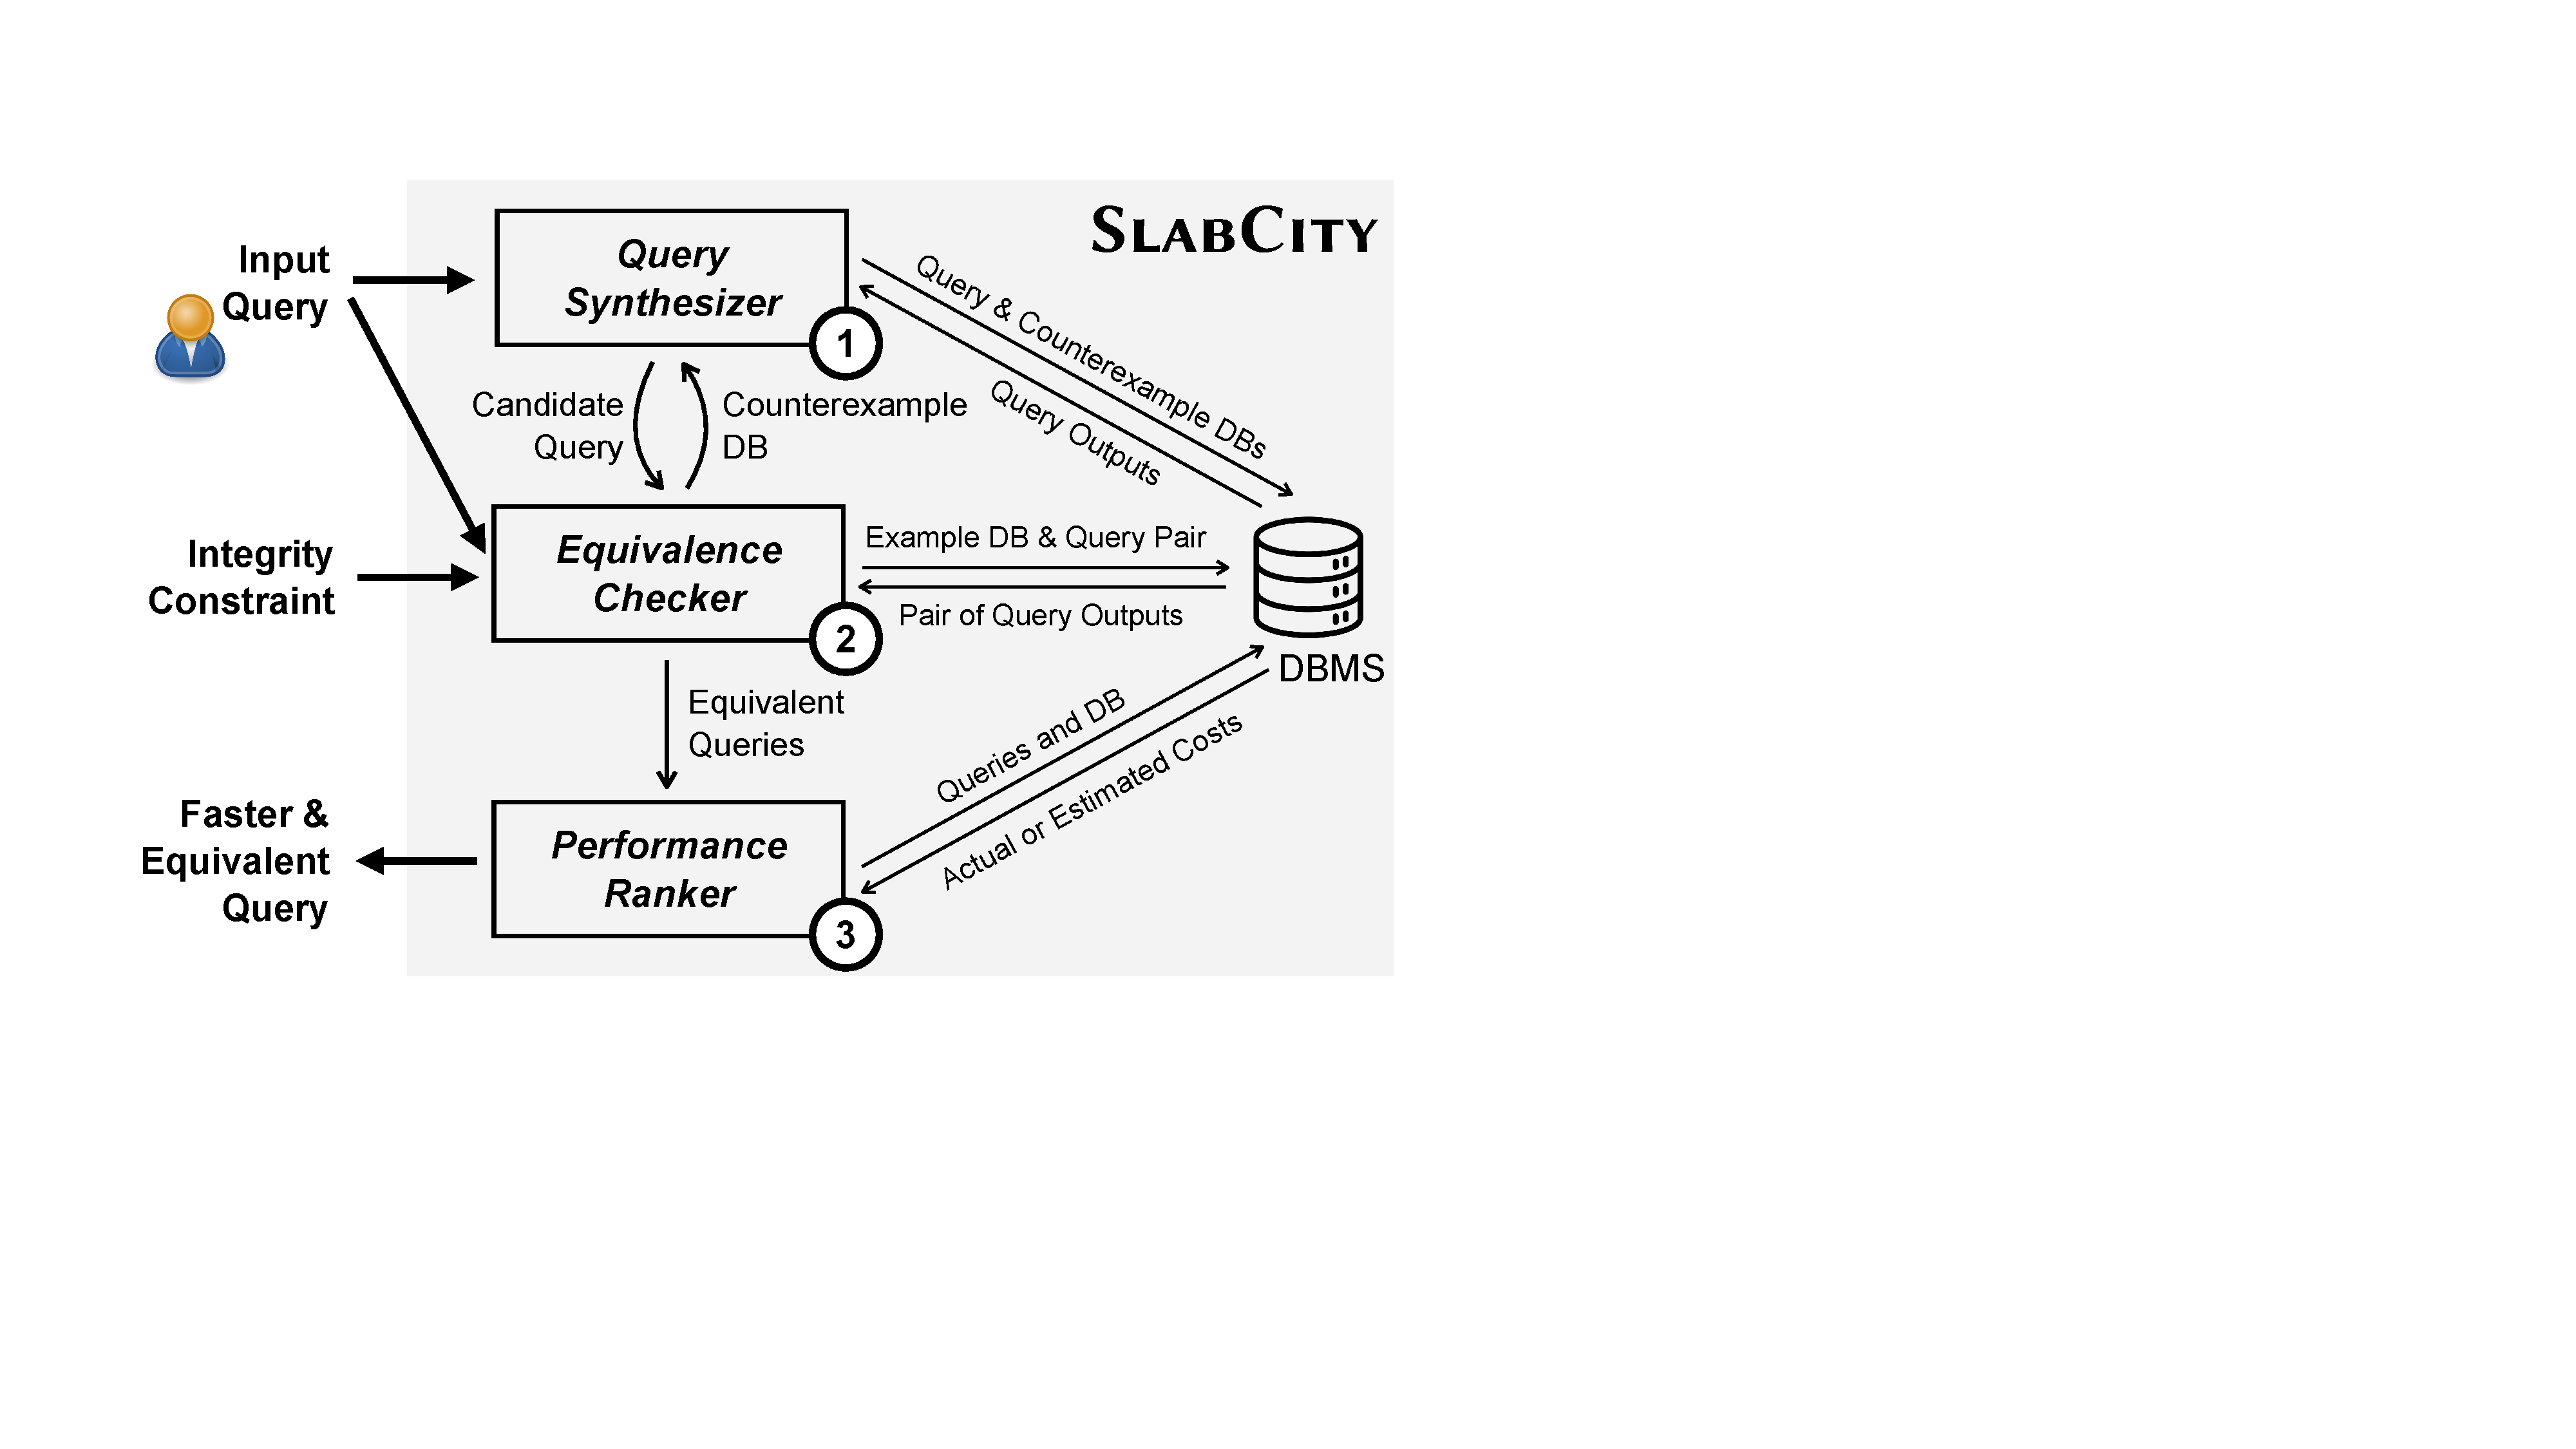
\includegraphics[width=0.8\linewidth]{chapters/slabcity/figs/workflow-clean.pdf}
\vspace{-5pt}
\caption{Schematic workflow of \slabcity.}
\vspace{-10pt}
\label{slab:fig:workflow}
\end{figure}

At the system level, \slabcity takes a query and the integrity
constraints of its schema and returns a semantically equivalent query
expected to run faster. \Cref{slab:fig:workflow} shows the
architecture, which instantiates the counterexample-guided inductive
synthesis (CEGIS) loop introduced in Chapter~2. A dataflow-guided
synthesizer proposes candidates that agree with the input query on all
counterexample databases collected so far. Each candidate then faces
the layered equivalence checker: a fast tester that hunts for a
distinguishing database, a bounded verifier that proves agreement on
all small inputs, and a full verifier that, when it succeeds within
its budget, establishes equivalence outright. A candidate refuted by
the tester or by the bounded verifier yields a new counterexample
database that sharpens the synthesizer's next proposals; a refutation
by the full verifier arrives as a verdict rather than a witness, and
simply discards the candidate. A candidate that survives is labeled
with the strongest guarantee it earned: fully verified, verified on
all bounded inputs, or, when the verifiers cannot reach a conclusion
within their budgets, tested. Surviving candidates are ranked by
measured or estimated latency, and the fastest is returned with its
label; a fully verified rewrite can be deployed as is, while the
weaker labels route the rewrite for human inspection.

\slabcity is aimed at workloads where a few seconds of one-time search
effort is negligible against the query's lifetime cost. That covers
queries written once and executed indefinitely, dashboards and the
query templates embedded in database-backed applications, and it
covers long-running analytical queries, where even a single execution
dwarfs a five-second rewriting budget. In both settings the rewriter
runs as a deployment-time step, after the query is written and before
it enters service. The supported language is an expressive subset of
SQL, including nested subqueries and arbitrary join structure; the
formal definition appears in \cref{slab:sec:problem}.

In summary, this chapter makes the following contributions:
\begin{itemize}[leftmargin=*]
\item
It introduces query dataflows: a semantic abstraction of SQL queries,
an algorithm for extracting the dataflows a query manifests, and the
observation that equivalent queries share dataflows, which converts an
undirected search space into a navigable one (a contribution of this
dissertation).
\item
It presents \slabcity, the first synthesis-based rewriter capable of
whole-query optimization with no rewrite rules, combining
dataflow-guided synthesis (due to Rui Dong, summarized here) with
layered equivalence checking (joint work).
\item
It contributes a benchmark of more than 1{,}000 real-life queries
curated from LeetCode, supporting research on query rewriting beyond
this chapter (joint work).
\item
It evaluates \slabcity against state-of-the-art rule-based and learned
rewriters across four workloads, showing that it optimizes 7 to 68\%
more queries and produces rewrites up to four orders of magnitude
faster (joint work).
\end{itemize}

The rest of the chapter proceeds as follows.
\Cref{slab:sec:motivating-example} illustrates, through queries drawn
from real workloads, the rewrites that rule-based systems miss and
this chapter's approach finds. \Cref{slab:sec:problem} defines the
query language and the rewriting problem precisely.
\Cref{slab:sec:dataflow} develops the dataflow abstraction, the
technical core of the chapter. \Cref{slab:sec:synthesis} summarizes
how the synthesis algorithm consumes dataflows to drive the search,
and \cref{slab:sec:eval} presents the evaluation. Related work,
including the two prior systems that apply synthesis to query
rewriting under rule-based or locality
restrictions~\cite{zhou2021sia,wang2022optimizing}, is discussed in
\cref{chap:related}.

\section{Motivating Examples}
\label{slab:sec:motivating-example}

In this section, we present a few examples to highlight the inherent limitations of rule-based 
query rewriting techniques and motivate the need for a synthesis-based whole-query optimization approach. 


All examples in this section are from two workloads: (1) real-life queries written by LeetCode users, 
%\footnote{The world's most popular online programming platform: https://leetcode.com/} users, 
and (2) benchmark queries from the Apache Calcite project~\cite{calcite}.
%\footnote{https://calcite.apache.org/}. 
We later present more comprehensive experiments on both workloads among others in Section~\ref{slab:sec:eval}. 
%but here we only use a handful of them as motivating examples.

\head{Example 1. Optimization with window functions} 
Consider LeetCode problem \#1308: a competition is held among teams of different genders. Given the table called \texttt{scores} with three columns \texttt{(gender,day,score)} where \texttt{(gender,day)} is the primary key, the goal is to find the running total score for each gender on each day. 
$\query_1$ in Table~\ref{slab:tab:Q1-Q2}  is the human-written solution for this problem (submitted by LeetCode participants) while 
$\query_2$ is \slabcity's automatically generated query after rewriting $\query_1$. 
$\query_2$ is more than 2000x faster than $\query_1$ on a database randomly populated with 1 million rows. 

\begin{table}[!t]
\footnotesize
\caption{$\query_1$ is human-written. $\query_2$ is generated by $\slabcity$.}
\vspace{-5pt}
\begin{tabular}{|c|c|}
\hline
 $\query_1$

 & 
 
 \makecell[l]{\sqlselectcolor \  \sqldistinctcolor s1.gender, s1.day, \sqlsumcolor(s2.score)\\
              \sqlfromcolor scores \sqlascolor s1 \sqljoincolor scores \sqlascolor s2 \\
              \hspace{2em} \sqloncolor s1.gender = s2.gender\\
              \sqlwherecolor s2.day <= s1.day \\
              $\sqlgroupbycolor$ s1.gender, s1.day
              }  
\\
\hline
$\query_2$
&
 \makecell[l]{ \sqlselectcolor gender, day, \\ \hspace{1em} \sqlsumcolor(score) \sqlovercolor (\sqlpartitionbycolor gender \sqlorderbycolor day) \\
 \sqlfromcolor scores}
  \\
 \hline
\end{tabular}
% \vspace{5pt}

\vspace{-5pt}
\label{slab:tab:Q1-Q2}
\end{table}



$\query_1$ is slow for two reasons. First, it uses a self-join to compute the running total, which generates a massive intermediate result. 
The same running total can be obtained using a window function as shown in $\query_2$. Second, the use of \sqldistinctcolor in $\query_1$ is redundant, since \texttt{(gender,day)} is the primary key. 

%\head{Limitations of rule-based techniques}

It is difficult to express any local rewrite rule to do this kind of optimization for $\query_1$ because nearly every part of the query would have to change. Moreover, anticipating these kinds of patterns in advance and writing a rule for each would be tedious (if not impossible). 
Even if one can create rules for a query like $\query_1$, many constraints would need to be met to ensure correctness, necessitating a potentially very complex pattern-matching. 
%and a very complex pattern matching would be needed. 
However, \slabcity's synthesis-based optimization can deal with such cases easily because, instead of doing constraint checking and pattern-matching, \slabcity~\emph{directly} searches the query language (as defined in Figure~\ref{slab:fig:querysyntax}),
allowing it to discover semantically equivalent and faster queries that may be quite different \emph{syntactically}. 
For these reasons, none of the state-of-the-art rule-based rewriters, such as {\learnedrewrite} (\LR)~\cite{LR} and {\wetune} (\WT)~\cite{wetune}, were able to optimize $\query_1$.\footnote{We explain how these state-of-the-art query rewriters work in more detail and report comprehensive experimental results in Section~\ref{slab:sec:eval}.}


%We will also use $(\query_1, \query_2)$ as a running example in Section~\ref{slab:sec:alg} to help illustrate details of our technique. 


\head{Example 2. Exploiting integrity constraints} 
The following is LeetCode problem \#1821.  
Given table \texttt{customers} with columns \texttt{(cid,year,revenue)} and \texttt{(cid,year)} as its primary key, the goal is to report  customers with positive revenue in  the year 2021. 
$\query_3$ from Table~\ref{slab:tab:Q3-Q4} is the human-written solution\footnote{While a database expert might be surprised why the user missed the integrity constraint and wrote such an inefficient query in the first place, situations like this are quite common in the industry for two reasons: (1) most queries are rewritten by users who are not SQL proficient, such as business users and financial analysts~\cite{slow-query-impact-5,slow-query-impact-7}
% ~\cite{Jie/Rui plz find a lot of links online to posts where ppl complain about poorly written SQL queries and cite them here} \xinyu{Jie: add cites here?} \jie{working on this}
, and (2) modern warehouses have hundreds of tables, and the knowledge of the schema and integrity constraints are thus scattered across different teams, especially in larger organizations~\cite{arora2011schema,stein2014enterprise}.
% ~\cite{Jie/Rui see if you can find some links supporting this. i know this is true anecdotally}. \xinyu{Jie/Rui: add cites?} \jie{working on this}
}  
for this task, while 
$\query'_4$ and $\query_4$ are $\slabcity$'s automatically generated queries for $\query_3$, which 
are  1.27x and 5.47x faster respectively (on a database with 1M rows).
$\slabcity$ can generate both $\query_4'$ and $\query_4$ but returns the latter due to its superior performance.

\begin{table}[!t]
\footnotesize 
\caption{$\query_3$ is human-written. $\query'_4$ and $\query_4$ are discovered by \slabcity ($\query_4$ is the final output as its faster than $\query'_4$).}
\vspace{-5pt}
\begin{tabular}{|c|c|}
\hline
 $\query_3$

 & 
 
 \makecell[l]{\sqlselectcolor cid\\
 \sqlfromcolor (\sqlselectcolor cid, \sqlsumcolor(revenue) \\ 
 \hspace{7.2em} \sqlovercolor (\sqlpartitionbycolor cid, year) \sqlascolor r \\
             \hspace{2.3em} \sqlfromcolor customers \  \sqlwherecolor year = 2021) \sqlascolor tmp \\
               \sqlwherecolor r > 0
              }  
\\

\hline

$\query_4'$

&

 \makecell[l]{ \sqlselectcolor cid \ \sqlfromcolor customers \ \\ \sqlwherecolor year = 2021 \\ 
                $\sqlgroupbycolor$ cid \  \sqlhavingcolor \sqlsumcolor(revenue) > 0}
 
 \\

 
\hline
$\query_4$
&
 \makecell[l]{
 \sqlselectcolor cid \ 
 \sqlfromcolor customers \\ 
 \sqlwherecolor year = 2021 \sqlandcolor revenue > 0
              }  
  \\
  
 \hline
\end{tabular}
\vspace{-8pt}

% \vspace{-20pt}
\label{slab:tab:Q3-Q4} 
\end{table}

%Capturing this kind of rewrite for rule-based techniques is inherently difficult as their ability to exploit integrity constraints is rather weak. For example, they are comfortable with checking if a single column is primary key so that a specific rule can be applied but they cannot infer if a single column (not primary key) is unique given a set of integrity constraints, which requires reasoning ability. As a result, syntactic pattern matching needs to be used more heavily to make up for their weak constraint checking, which is error-prone and still incomplete. In contrast, since \slabcity is not restricted to rules, as long as there is an optimal query in the search space, it will eventually find it.


$\query_3$ is slow because it uses an unnecessary window function with $\sqlpartitionbycolor$. $\query'_4$ achieves the same goal faster by replacing the window function with aggregation and $\sqlgroupbycolor$. This is because \texttt{(cid,year)} is the primary key --- once \texttt{year} is fixed, there is only a tuple for each unique value of \texttt{cid}. 
That is, partitioning by \texttt{(cid,year)} and grouping by \texttt{cid} when  \texttt{year=2021} leads to the same groups. 
Exploiting this integrity constraint further, 
\slabcity is able to find an even more optimized query $\query_4$.
This is because 
each \texttt{(cid,year)} will also determine a unique \texttt{revenue}, making the summation unnecessary.  
However, none of the state-of-the-art rule-based techniques could optimize or even rewrite $\query_3$ to anything. 
Capturing this kind of rewrite for rule-based techniques is nearly impossible, as they heavily rely on pattern-matching and their ability to exploit integrity constraints is largely limited to local changes (e.g., removing redundant grouping columns or redundant left joins).
In contrast, because \slabcity is  not restricted to rewrite rules fundamentally, as long as there is a better query in the query space, it will eventually find it. 



\head{Example 3. Eliminating redundant joins} 
Calcite comes with a rich set of test cases to check if its rewrite rules function properly.
$\query_5$ in Table~\ref{slab:tab:Q5-Q7} is one of those test cases (``testPushAggregateThroughOuterJoin14'') where 
Calcite rewrites $\query_5$ to  $\query_6$. Here, \texttt{emp} is a table with three columns \texttt{(empno,ename,mgr)} with \texttt{empno} as its primary key. 
$\query_5$ performs a full self-join of \texttt{emp} on the \texttt{mgr} column, grouped by the join key. This is 
essentially equivalent to using \sqldistinctcolor to return only distinct values. 
$\query_6$ is the optimized query using Calcite rules, which is 926x faster than $\query_5$ on a database with 4M rows. $\query_7$ is the query  automatically generated by \slabcity, which is 1833x faster than $\query_5$ on the same database. 


\begin{table}[!t]
\footnotesize
\caption{$\query_5$ is a test query from Calcite, 
$\query_6$ is the rewritten version of $\query_5$ using Calcite rules, and
$\query_7$ is \slabcity's output.}
\vspace{-8pt}
\begin{tabular}{|c|c|}
 \hline
 $\query_5$ 

 & 
 
 \makecell[l]{\sqlselectcolor e0.mgr \sqlascolor mgr0, e1.mgr \sqlascolor mgr1 \\
             \sqlfromcolor emp \sqlascolor e0 \sqlfulljoincolor emp \sqlascolor e1 \sqloncolor e0.mgr = e1.mgr\\
              $\sqlgroupbycolor$ e0.mgr, e1.mgr
              }  
\\

\hline

 $\query_6$ 

 & 
 
 \makecell[l]{\sqlselectcolor e0.mgr \sqlascolor mgr0, e1.mgr \sqlascolor mgr1 \\
             \sqlfromcolor (\sqlselectcolor mgr \sqlfromcolor emp $\sqlgroupbycolor$ mgr) \sqlascolor e0\\
            \hspace{1em} \sqlfulljoincolor (\sqlselectcolor mgr \sqlfromcolor emp $\sqlgroupbycolor$ mgr)  \sqlascolor e1 \\
            \hspace{1em} \sqloncolor e0.mgr = e1.mgr\\
              $\sqlgroupbycolor$ e0.mgr, e1.mgr
              }  
\\

\hline

 $\query_7$ 

&

 \makecell[l]{\sqlselectcolor mgr \sqlascolor mgr0, mgr \sqlascolor mgr1 \\
             \sqlfromcolor emp \\ $\sqlgroupbycolor$ mgr
              }  
\\
 \hline
\end{tabular}


\vs
\label{slab:tab:Q5-Q7} 
\vspace{5pt}
\end{table}

$\query_6$ is significantly faster than $\query_5$ because pushing $\sqlgroupbycolor$ before the self-join leads to  significantly smaller join operands and thus a more efficient execution; however, this is still not the best rewrite possible. Interestingly, self-join can be eliminated altogether in this case, leading to an even more significant speed-up, which is exactly what \slabcity does by rewriting $\query_5$ into $\query_7$. 
In fact, this is not limited to Calcite:
none of the state-of-the-art rule-based query rewriters found this opportunity,\footnote{Similar to Calcite, LearnedRewrite~\cite{LR} was only able to rewrite $\query_5$ into $\query_6$ but did not eliminate the self-join. WeTune was not able to rewrite $\query_5$ at all.} 
simply because they fail to capture the information that the joined columns may come from the same table and hence be identical --- a fact that could be exploited to eliminate redundancy. 
Similar to Examples 1 and 2, it is tedious, if not impossible, to create rewrite rules for this type of optimization.
In particular, identifying self-joins requires semantic information that the two joined operands are essentially the same relation. Even if one wrote a very specific rule for\\
\texttt{\sqlfromcolor T AS T1 \sqljoincolor T AS T2}\\
to find self-joins syntactically, they would still miss out on queries expressed as \\
\texttt{\sqlfromcolor T AS T1 \sqljoincolor (\sqlselectcolor * from T) AS T2} \\ 
In contrast, because of using query synthesis, $\query_7$ is naturally within \slabcity's search space and \slabcity can successfully find it as a query with minimal redundancy and best performance.




\begin{table}[!t]
\footnotesize
\caption{$\query_8$ is a test query from Calcite, 
$\query_9$ is the rewrite using Calcite rules, and
$\query_{10}$ is \slabcity's output.}
\vspace{-8pt}
\begin{tabular}{|c|c|}

 \hline
 $\query_8$

 & 
\makecell[l]{\sqlselectcolor ename, \sqlmincolor (empno) \sqlascolor e \sqlfromcolor (\\
             \hspace{1em} \sqlselectcolor * \sqlfromcolor emp \\
             \hspace{1em} \sqlunionallcolor\\
             \hspace{1em} \sqlselectcolor * \sqlfromcolor emp\\
              ) \sqlascolor t $\sqlgroupbycolor$ ename
              } 
 
  
\\

 \hline
 $\query_9$

 & 
\makecell[l]{\sqlselectcolor ename, \sqlmincolor (e) \sqlascolor e \sqlfromcolor (\\
             \hspace{1em} \sqlselectcolor ename, \sqlmincolor (empno) \sqlascolor e \sqlfromcolor emp $\sqlgroupbycolor$ ename\\
             \hspace{1em} \sqlunionallcolor\\
             \hspace{1em} \sqlselectcolor ename, \sqlmincolor (empno) \sqlascolor e \sqlfromcolor emp $\sqlgroupbycolor$ ename\\
              ) \sqlascolor t $\sqlgroupbycolor$ ename
              } 
 
  
\\

\hline

 $\query_{10}$

&
\makecell[l]{\sqlselectcolor ename, \sqlmincolor (e) \sqlascolor e \\ \sqlfromcolor (\sqlselectcolor ename, \sqlmincolor (empno) \sqlascolor e
             \\ 
             \hspace{2.4em} \sqlfromcolor emp 
             \\ \hspace{2.4em} $\sqlgroupbycolor$ ename) \sqlascolor t
             \\
             $\sqlgroupbycolor$ ename
              } 
  
 
 \\
 \hline
\end{tabular}
\vspace{-15pt}


\label{slab:tab:Q8-Q10} 
\end{table}




\head{Example 4. Optimizating set operations}
$\query_8$ in Table~\ref{slab:tab:Q8-Q10} is yet another test case (``testPushMinThroughUnion'') from Calcite, 
which is rewritten to $\query_9$ using Calcite rules, slightly improving its latency ($\pm$2\%) by pushing $\sqlgroupbycolor$ past $\sqlunionallcolor$. 
On the other hand, \slabcity rewrites $\query_9$ to $\query_{10}$, which is 1.7x faster. 


Similar to Example 3, state-of-the-art rule-based rewriters fail to exploit the fact that both sides of $\sqlunionallcolor$ are identical, and thus fail to eliminate the redundant computation. 
In fact, neither \learnedrewrite nor \wetune were able to optimize $\query_8$ (the former could rewrite it to $\query_9$ whereas the latter was not even able to rewrite it to anything at all).
%\barzan{jie, plz go through the whole paper and see how we refer to LR and WT, do we use these acronyms everywhere? If so, let's define them the first timr we reference them and use the same everywehre consistently} \jie{We first use it in example 1 (page 3). I am not sure if I "define" it properly there. Please check}
Again, because $\slabcity$ uses query synthesis, it is able to find $\query_{10}$ which is both equivalent and faster.


\head{Discussion}
In our evaluation, we have come across many other interesting examples where state-of-the-art query rewriting techniques were not able to optimize the input query or even rewrite it at all, while \slabcity could (see Section~\ref{slab:sec:q1-coverage}).
Even when they were able to optimize the query, \slabcity's output oftentimes was significantly faster (see Section~\ref{slab:sec:q2-reduction}). 
Note that in this paper, we differentiate two terms \emph{optimize} vs. \emph{rewrite}: the former means the technique can rewrite the input query to an output query that is faster, whereas the latter means the technique can rewrite to some query which may or may not be faster. In other words, optimizing is harder than rewriting. 
Our intention of sharing these motivating examples in Section~\ref{slab:sec:motivating-example} is to demonstrate why it is inherently difficult and error-prone to create enough rules that can handle complex and unseen situations. In contrast, a synthesis-based approach does not need a supply of hard-coded rules and can discover optimization opportunities by searching the SQL language \emph{directly}.

\begin{comment}
\barzan{Xinyu, this is why i think its better to not use rewrite and optimize interchangeably. if you agree, plz add the clarification the first time it occurs that optimize means rewriting into a faster query.}
Even when they were able to optimize the query, \slabcity's output was significantly faster (see Section~\ref{slab:sec:??}). 
Interestingly, we even identified several examples where these techniques produced an incorrect query (see \barzan{appendix or tech report or supp material? if this stmt is not true then eliminate this sentence} \jie{this stmt is true and I think we can add some examples as the proof})
Our intention of sharing these motivating examples in this section to show the reader why it is inherently difficult, error-prone, and extremely difficult \jie{(inherently difficult, extremely difficult) repeat?} to create enough rules that can handle 
complex and unseen situations. In contrast, a synthesis approach does not need a supply of hard-coded rules and can discover optimization opportunities by searching the languauge space directly.
\barzan{Xinyu, reword or add this para if you want}
\end{comment}


\section{Problem Setup}
\label{slab:sec:problem}

This section fixes the search space and the goal: the query language
\toolname operates over, the integrity constraints it can exploit, and
the problem it solves.

%\subsection{Query Space}
%\label{slab:sec:querylanguage}

\head{Query space}
The language, defined in Figure~\ref{slab:fig:querysyntax}, is an
expressive subset of SQL covering arbitrary nesting and join
structure.
%\slabcity currently supports a wide subset of SQL queries, including arbitrary nesting and join patterns. See Figure~\ref{slab:fig:querysyntax} for the formal language currently supported by \slabcity.



%\subsection{Integrity Constraints}
%\label{slab:sec:integrityconstraints}

\head{Integrity constraints}
Constraints both shrink the space of databases against which
equivalence must hold and, as Example~2 of
\cref{slab:sec:motivating-example} illustrated, create rewrite
opportunities. \slabcity supports the following kinds:
\begin{itemize}[leftmargin=*]
\item 
Primary and foreign keys. 
\item 
Comparisons within a row --- e.g.,  $\texttt{T.StartTime} < \texttt{T.EndTime}$. 
\item 
Implication constraints within a row. For example, $\texttt{T.EmailType} \neq \emph{spam} \rightarrow \texttt{T.action} = \texttt{NULL}$. 
%means if column \texttt{EmailType} is not \emph{spam} then column \texttt{action} is \texttt{NULL}. 
\item 
Whether or not a column can be \texttt{NULL}. 
\item 
Range constraints (for columns of integer or numeric types).
\item 
Enum types (e.g., column \texttt{Device} can draw from \{ \emph{S8}, \emph{iPhone} \}).
\end{itemize}

\begin{comment}
\begin{enumerate}
    \item primary keys
    \item foreign keys
\item comparative constraints within a row, e.g. \texttt{T.StartTime < T.EndTime} 
    \item implication constraints within the same row, e.g. \texttt{T.EmailType != "spam" -> T.action = NULL} means if the value of column \texttt{EmailType} is not \texttt{"spam"}, then the value of column \texttt{action} is \texttt{NULL}
        \item whether or not a column can be \texttt{NULL}
    \item range constraints (for int or numeric type columns)
    \item enum types, e.g. column \texttt{Device} can only take values from the set \texttt{\{"S8", "iPhone"\}}
    %\item \tofix{special constraints within a column, including 1) values of a column are incremental, 2) values of a column are consecutive.} \barzan{this one is a bit strange, what is the actual name of this kind of constraint in Oracle? auto increment is a feature not an IC afaik}     \xinyu{I think this one is very rare in the benchmarks. we do not have to include this one in the list.}
\end{enumerate}
\end{comment}


\head{Problem statement}
With the language and constraints in place, the problem is the
following.
%\subsection{Query Optimization Problem Statement}
%\label{slab:sec:problemstatement}

\begin{definition}
Given a query $\inputquery$ and an integrity constraint $\dataconstraint$, find a query $\query$ from our query language, such that the following two conditions hold: 
\begin{enumerate}[leftmargin=*]
\item 
$\query$ is semantically equivalent to $\inputquery$ with respect to $\dataconstraint$. 
That is, $\query$ and $\inputquery$ produce the same output on any database $\inputdb$ that meets the integrity constraint $\integrityconstraint$. 
\item 
$\query$ runs faster than $\inputquery$. Here, query performance is measured using \texttt{EXPLAIN} or the actual execution of the query.
\end{enumerate}
\label{slab:def:problem}
\end{definition}

Two aspects of the definition deserve a remark. Equivalence is
relative to the constraints, which is what licenses rewrites like
$\query_4$ in \cref{slab:sec:motivating-example}: they would be wrong
on arbitrary databases and are right on the databases that can
actually occur. And the definition asks for a faster query, not just
an equivalent one, which is why the system must surface multiple
equivalent candidates and rank them (\cref{slab:sec:perfranking}),
rather than stop at the first equivalence it can prove.



\begin{figure}[!t]
\footnotesize
\centering
\[
\arraycolsep=1.5pt\def\arraystretch{1.1}
\begin{array}{rrll}

\emph{Query} & 
\query & 
\grammareq & 
\emph{an input table} \\ 
& & \ \ \ | &  
\sqlselect \sqlspace \targetlist \sqlspace \sqlfrom \sqlspace \query \sqlspace \sqlwhere \sqlspace \sqlpredicate \\ 
& & \ \ \ | &  
\sqlselect \sqlspace \targetlist \sqlspace \sqlfrom \sqlspace \query \sqlspace \sqlgroupby \sqlspace \cols \sqlspace \sqlhaving \sqlspace \sqlpredicate \\ 
& & \ \ \ | &  
\sqlselect \sqlspace \targetlist \sqlspace \sqlfrom \sqlspace \query \sqlspace \sqlorderby \sqlspace \cols  \\ 
& & \ \ \ | &  
\query \sqlspace \sqlinnerjoin \sqlspace \query \sqlspace \sqlon \sqlspace \sqlpredicate \\ 
& & \ \ \ | &  
\query \sqlspace \sqlleftjoin \sqlspace \query \sqlspace \sqlon \sqlspace \sqlpredicate 
%& & \ \ \ | &  
%\query \sqlspace \sqlrightjoin \sqlspace \query \sqlspace \sqlon \sqlspace \sqlpredicate 
\\[2pt]

\emph{Target List} & 
\targetlist & 
\grammareq & 
[ \target \sqlspace \sqlas \sqlspace \colalias, \mydots, \target \sqlspace \sqlas \sqlspace \colalias ]
\\
& & \ \ \ | &  
\sqldistinct \sqlspace [ \target \sqlspace \sqlas \sqlspace \colalias, \mydots, \target \sqlspace \sqlas \sqlspace \colalias ] 
%\rui{add DISTINCT?}
\\[2pt]

\emph{Target} & 
\target & 
\grammareq & 
\col \ | \ \agg(\col) \ | \ \agg( \sqldistinct \sqlspace \col) 
%\rui{add DISTINCT?} 
\\
& & \ \ \ | &  
\agg(\col) \sqlspace \sqlover( \sqlpartitionby \sqlspace \cols \sqlspace \sqlorderby \sqlspace \cols )
\\ 
& & \ \ \ | &  
\windowfunc \sqlspace \sqlover( \sqlpartitionby \sqlspace \cols \sqlspace \sqlorderby \sqlspace \cols )
\\[2pt] 

\emph{Column List} & 
\cols & 
\grammareq & 
[\col, \mydots, \col]
\\[2pt]

\emph{Column} & 
\col & 
\grammareq & 
\colalias \ | \ \emph{a column from an input table} 
\\[2pt]

\emph{Condition} & 
\sqlpredicate & 
\grammareq & 
\sqlexpr \ \emph{op} \ \sqlexpr \ | \ \sqlpredicate \land \sqlpredicate \ | \ \sqlpredicate \lor \sqlpredicate 
\\[2pt] 

\emph{Expression} & 
\sqlexpr & 
\grammareq & 
\col \ | \ \agg(\col) \ | \ \agg(\sqldistinct \sqlspace \col) \ | \ \emph{const}
\\[2pt] 

\emph{Agg. Func.} & 
\agg & 
\grammareq & 
\sqlmax \ | \ \sqlmin \ | \ \sqlavg \ | \ \sqlsum \ | \ \sqlcount 
\\[2pt] 

\emph{Window Func.} & 
\windowfunc & 
\grammareq & 
\sqldenserank \ | \ \sqlrank 
\\[2pt] 

\end{array}
\]
\vspace{-15pt}
\caption{Syntax of our query language.}
\label{slab:fig:querysyntax}
\vspace{-20pt}
\end{figure}



\section{Synthesis-Aided Query Optimization}
\label{slab:sec:alg}


\revisioncancut{Section~\ref{slab:sec:toplevelalg} first presents a high-level overview of our synthesis-aided query optimization algorithm. 
Subsequent sections present the technical details of each component. 
We define dataflows for SQL queries --- which is one of our key contributions --- and use that to develop a monotonic scoring in Section~\ref{slab:sec:scorefunction}.
Section~\ref{slab:sec:prioritizingsearch} presents our query search algorithm. 
Finally, we describe how we check for equivalence and rank queries in  Sections~\ref{slab:sec:checkingequiv} and~\ref{slab:sec:perfranking}, respectively.}

 
\newcounter{mycounter}


\subsection{Top-Level Algorithm}
\label{slab:sec:toplevelalg}
Our top-level algorithm is shown in Algorithm~\ref{slab:alg:toplevelalg}. It accepts as input a query $\inputquery$ and an integrity constraint $\integrityconstraint$, and returns an output query $\query$ that is semantically equivalent to and faster than $\inputquery$. 
%In other words, if $\query$ passes our equivalence checker (line~\ref{slab:alg:toplevelalg:checkequiv}) and is ranked as faster than $\inputquery$ (line~\ref{slab:alg:toplevelalg:checkfaster}), then we return $\query$ at line~\ref{slab:alg:toplevelalg:returnquery}\footnote{For simplicity of our notation, here we only return the fastest query but one can also return the entire ranked list of rewritten queries to the user.}.
$\query$ is $\bot$ if it does not find one such query within the given time limit. 




Let us explain Algorithm~\ref{slab:alg:toplevelalg} in more detail. At a high-level, our algorithm is a \emph{new instantiation} of the counterexample-guided inductive synthesis (CEGIS) paradigm~\cite{solar2008program} --- which has found great success in the programming languages community --- for our query optimization problem. 
Our approach consists of (a) an inductive synthesizer (i.e., our query synthesizer) that aims to find a query $\query$ which satisfies a set $\counterexamples$ of \emph{counterexamples} and (b) a query checker (i.e., our equivalence checker) which checks whether or not $\query$ is equivalent to $\inputquery$ and generates a counterexample $\counterexample$ if not. 
One key advantage of using CEGIS is to enable efficient checking: checking a candidate query against $\counterexamples$ (line~\ref{slab:alg:toplevelalg:satisfycounterexample}) is typically significantly cheaper than calling an equivalence checker (line~\ref{slab:alg:toplevelalg:checkequiv}, e.g., \spes~\cite{zhou2022spes}). In other words, verification is used parsimoniously only when necessary. 
In our context, a counterexample $\counterexample$ is an input DB together with the desired output table returned by $\inputquery$. 




{In addition to using counterexamples, \toolname also uses a novel $\scorefunction$ function that defines dataflows for queries in order to guide the query synthesis process. 
While we defer the formal definition of $\scorefunction$ to Section~\ref{slab:sec:scorefunction}, from a high-level, it assigns a non-positive integer score\footnote{While \emph{non-positive} scores may seem counter-intuitive, they can be viewed as the negation of the cost, i.e., the higher the score, the lower the cost.} to each query $\query$ such that,  
$\query$ with a higher score is more likely to be an optimized query (i.e., semantically equivalent to and faster than $\inputquery$) and vice versa. 
Initially, $\counterexamples$ has no counterexamples and $\queryset$ is a empty set that stores equivalent queries (line~\ref{slab:alg:toplevelalg:init}). 
Then, we enter a CEGIS loop (lines~\ref{slab:alg:toplevelalg:whilebegin}--\ref{slab:alg:toplevelalg:whileend}). At line~\ref{slab:alg:toplevelalg:forloop}, it \emph{lazily} enumerates all queries in non-ascending order of their scores. In other words, $\toolname$ prioritizes the search for candidate queries $\query$ that are likely to optimize $\inputquery$ (i.e., with a higher score). 
Line~\ref{slab:alg:toplevelalg:satisfycounterexample} checks if $\query$ meets $\counterexamples$: if not, it continues to the next candidate. 
If $\query$ passes $\counterexamples$, we invoke the equivalence checker (line~\ref{slab:alg:toplevelalg:checkequiv}) to see if $\query$ is equivalent --- it returns a new counterexample $\counterexample$ if not equivalent, or returns $\emph{null}$ otherwise. 
For the latter case, line~\ref{slab:alg:toplevelalg:nocounterexample} adds $\query$ to $\queryset$; for the former, line~\ref{slab:alg:toplevelalg:addcounterexample} adds  $\counterexample$ to $\counterexamples$.
Upon termination, we rank queries in $\queryset$ (line~\ref{slab:alg:toplevelalg:checkfaster}) and return a ``best'' query that we believe can \emph{optimize} $\inputquery$.}



\begin{figure}[!t]
\vspace{-5pt}
\footnotesize
\centering

\begin{algorithm}[H]
\begin{algorithmic}[1]

\myprocedure{Optimize}{$\inputquery, \integrityconstraint$}

\Statex\Input{An input query $\inputquery$ and an integrity constraint $\integrityconstraint$.}


\Statex\Output{An equivalent and faster output query $\query$.}

\vspace{2pt}

\State $\counterexamples \assign \emptyset$; \  $\queryset \assign \emptyset$; 
\label{slab:alg:toplevelalg:init}



\While{not timed out}
\label{slab:alg:toplevelalg:whilebegin} 



\ForAll{$\query \in \textsc{LazyEnumerate}(\inputquery)$} \label{slab:alg:toplevelalg:forloop}
\Comment{{{\scriptsize \Circled{1}}} Query synthesizer.}


\State \textbf{if} $\query$ doesn't pass  $\counterexamples$ \textbf{then} \textbf{continue}; \label{slab:alg:toplevelalg:satisfycounterexample}
\Comment{Check against counterexs.}


\State $\counterexample \assign \textsc{CheckEquivalence}(\query, \inputquery, \integrityconstraint)$;\label{slab:alg:toplevelalg:checkequiv}
\Comment{{{\scriptsize \Circled{2}}} Equivalence checker.}

\vspace{1pt}

\If{$\counterexample = \emph{null}$} 
$\queryset.\emph{add}(\query)$
\label{slab:alg:toplevelalg:nocounterexample}
\Comment{$\emph{null}$ means $\query$ is equivalent to $\inputquery$.}

\Else \ $\counterexamples.\emph{add}( \counterexample )$;
\Comment{Otherwise, $\counterexample$ is a new counterexample.}
\label{slab:alg:toplevelalg:addcounterexample}

\EndIf

\EndFor


\EndWhile
\label{slab:alg:toplevelalg:whileend}

\vspace{-1pt}
\State $\query \assign \textsc{RankPerformance}(\queryset, \inputquery)$;
\label{slab:alg:toplevelalg:checkfaster}
\Comment{{{\scriptsize \Circled{3}}} Performance Ranker.}

\State \Return $\query$;
\label{slab:alg:toplevelalg:returnquery}

\caption{{Top-level algorithm of \toolname.}}
\label{slab:alg:toplevelalg}
\end{algorithmic}
\end{algorithm}
\vspace{-10pt}
\end{figure}





\begin{comment}
    
\begin{figure}[!t]
\small 
\centering

\begin{algorithm}[H]
\begin{algorithmic}[1]

\myprocedure{Optimize}{$\inputquery, \integrityconstraint$}

\Statex\Input{An input query $\inputquery$ and an integrity constraint $\integrityconstraint$.}


\Statex\Output{An equivalent and faster output query $\query$.}

\vspace{2pt}

\State $\counterexamples \assign \emptyset$; \  $\cost = 0; \ \queryset \assign \emptyset$; 
\label{slab:alg:toplevelalg:init}



\While{not timed out}
\label{slab:alg:toplevelalg:whilenottimeout} 



\ForAll{$\query \in \textsc{LazyEnumerate}(\cost)$} \label{slab:alg:toplevelalg:forloop}
\Comment{{{\scriptsize \Circled{1}}} Query synthesizer.}


\State \textbf{if} $\query$ doesn't pass  $\counterexamples$ \textbf{then} \textbf{continue}; \label{slab:alg:toplevelalg:satisfycounterexample}
\Comment{Check against counterexs.}


\State $\counterexample \assign \textsc{CheckEquivalence}(\query, \inputquery, \integrityconstraint)$;\label{slab:alg:toplevelalg:checkequiv}
\Comment{{{\scriptsize \Circled{2}}} Equivalence checker.}

\vspace{1pt}

\If{$\counterexample = \emph{null}$} 
$\queryset.\emph{add}(\query)$
\label{slab:alg:toplevelalg:nocounterexample}
\Comment{$\emph{null}$ means $\query$ is equivalent to $\inputquery$.}

\Else \ $\counterexamples.\emph{add}( \counterexample )$;
\Comment{Otherwise, $\counterexample$ is a new counterexample.}
\label{slab:alg:toplevelalg:addcounterexample}

\EndIf

\EndFor

\vspace{-2pt}
\State $\cost \assign \cost - 1$;
\label{slab:alg:toplevelalg:decreasescore} 

\EndWhile

\vspace{-1pt}
\State $\query \assign \textsc{RankPerformance}(\queryset, \inputquery)$;
\label{slab:alg:toplevelalg:checkfaster}
\Comment{{{\scriptsize \Circled{3}}} Performance Ranker.}

\State \Return $\query$;
\label{slab:alg:toplevelalg:returnquery}

\caption{Top-level algorithm of \toolname.}
\label{slab:alg:toplevelalg}
\end{algorithmic}
\end{algorithm}
\vspace{-20pt}
\end{figure}

\end{comment}



\begin{example}
Suppose $\inputquery$ is query $\query_1$ from Table~\ref{slab:tab:Q1-Q2}. 
Our CEGIS-based algorithm will begin with query candidates with score 0: $\query'$ below is one such query. 
$\query'$ is obviously not equivalent to $\inputquery$, and our equivalence checker gives a counterexample $\counterexample$ below. Note that $\counterexample$ consists of an input DB $\inputdb$ and the output that $\inputquery$ returns on $\inputdb$. 
A query eventually returned by our tool will pass this counterexample. 



\begin{table}[H]
\footnotesize
\caption*{A counterexample $\counterexample$ consists of an input database $\inputdb$ (left) and an output table of $\inputquery$ on $\inputdb$.}
\vspace{-7pt}
\hspace*{-5pt}
\begin{tabular}{cc}
\makecell[l]{ $\query': $ \ \sqlselectcolor gender, day, \\  
\hspace{42pt} \sqlsumcolor(score) 
  \\ \hspace{2em} \sqlfromcolor scores
  \\ \hspace{2em} $\sqlgroupbycolor$ gender, day}
  &
\makecell[l]{ $\query\doubleprime: $ \sqlselectcolor gender, day, \\
\hspace{5.3em} \sqlsumcolor(score) \\  \hspace{5.3em} \sqlovercolor ($\sqlpartitionbycolor$ gender \\ \hspace{7.9em} $\sqlorderbycolor$ day)\\
 \hspace{2em}  \  \sqlfromcolor scores \\ \hspace{2em} \  $\sqlgroupbycolor$ gender, day}
\end{tabular}
\vspace{-12pt}
\end{table}



\begin{table}[H]
\footnotesize
\begin{tabular}{cc}
\begin{subtable}{.4\linewidth}
\begin{tabular}{|c|c|c|}
 \hline
        gender & day & score \\
        \hline
        a & 1 & 1 \\
        a & 2 & 2 \\
        \hline
\end{tabular}
\end{subtable}
&
\begin{subtable}{.4\linewidth}
\begin{tabular}{|c|c|c|}
 \hline
        gender & day & score \\
        \hline
        a & 1 & 1 \\
        a & 2 & 3 \\
        \hline
\end{tabular}
\end{subtable}
\end{tabular}
%\caption{counterexample $\counterexample$}

\vspace{-5pt}
\label{slab:tab:alg:counterexample}
\end{table}



On the other hand, the query $\query\doubleprime$ next to $\query$ above is equivalent to $\inputquery$. However, $\query\doubleprime$ is determined to be slower than $\query_2$ from Table~\ref{slab:tab:Q1-Q2} by our performance ranker. 
$\toolname$ was able to find both $\query_2$ and $\query\doubleprime$ which are added to $\queryset$; however, \toolname returns $\query_2$ in the end, since it is ranked the highest. 


\label{slab:ex:cegis}
\end{example}


\subsection{Dataflow-Based Query Score Function}
\label{slab:sec:scorefunction}

As we can see, a key challenge underlying the success of Algorithm~\ref{slab:alg:toplevelalg} is how to design a good score function as well as how to develop an algorithm that can effectively use the score function to prioritize the search. 
This section first addresses the score function design. 


\head{Key idea: scoring queries based on dataflows}
Recall that we use a score function to quantitatively rank queries in terms of their likelihood of optimizing a user-provided input query $\inputquery$. That is, given $\inputquery$ and $\query$, a desired score function should assign $\query$ with a higher score if $\query$ is indeed semantically equivalent to and faster than $\inputquery$. At the same time, it should minimize false positives: that is, it should not assign high scores to too many inequivalent queries. 


To design such a score function, our key insight is that, a query $\query$ that indeed optimizes $\inputquery$ typically exhibits \emph{dataflows} that are also manifested in $\inputquery$. 
For example, if $\query$ filters an aggregated column (e.g., using $\sqlhaving \sqlspace \sqlsum$), the same computations (e.g., calculating $\sqlsum$) likely would also show up in $\inputquery$, although the computations might be organized \emph{syntactically differently} (e.g., first calculating $\sqlsum$ in $\sqlselect$ and then using $\sqlwhere$ to filter, which is slower). 
In other words, our dataflow-based score function is designed to favor queries $\query$ that involve dataflows from $\inputquery$ --- the rationale is that, since $\inputquery$ is functionally correct, its underlying computations are likely sufficient for generating an optimized query.


However, we do not require $\query$ to use up all dataflows from $\inputquery$. In other words, $\inputquery$ may exhibit redundant dataflows that are not necessary for computing the same result and thus can be optimized away. For example, if $\inputquery$ involves a redundant $\sqljoin$, an optimized query $\query$ may contain only dataflows from one branch of the $\sqljoin$. 


Finally, if a query $\query'$ contains dataflows that are not exhibited in $\inputquery$, oftentimes $\query'$ is not equivalent and hence we can assign it with a lower score. For example, suppose $\inputquery$ calculates $\sqlsum$ over a column. It is less likely that a query $\query'$ can accomplish the same goal with only $\sqlavg$. Similarly, if $\inputquery$ and $\query'$ both perform filtering but on two different columns that are unrelated, it is more plausible to believe they are not semantically equivalent. 
%However, special care needs to be taken for ``alternative dataflows'' --- that is, two syntactically different dataflows may share the same underlying logic. 
%For instance, $\sqlpartitionby$ and $\sqlgroupby$, while syntactically different, can both be used for grouping. 



\barzanrev{Note that, 
since our score is calculated based on semantic information (i.e., dataflows) instead of syntactic features, a syntactically simpler query (e.g., one with fewer lines) may receive a lower score than a more complex query. 
In other words, our algorithm first prioritizes generating queries with higher scores, and 
then prioritizes syntactically smaller queries when their scores are the same (see Section~\ref{slab:sec:prioritizingsearch}). This is an advantage since it will allow us to uncover non-trivial rewrites sooner if they are more promising.} 


\head{Dataflows}
Our observations suggest a score function design that takes two queries (i.e., $\inputquery$ to be optimized and $\query$ to be scored), extracts dataflows for each, and calculates the score based on these dataflows. 
In what follows, we first formalize the notion of dataflow.
Then, we present the dataflow extraction algorithm. 

\begin{definition}[Dataflow]
A dataflow $\dataflowchain$ (defined in Figure~\ref{slab:fig:dataflowlanguage}) for a given query $\query$ is a sequence of SQL operations that are performed during $\query$'s execution on one or more input tables or their columns.
\end{definition}


Let us explain our dataflow language more formally (see Figure~\ref{slab:fig:dataflowlanguage}).
In the base cases, a dataflow $\dataflowchain$ is either an input table $\dbtable$ or a column from an input table. 
%it must not be a column alias created for an intermediate table. 
%The reason is to make dataflows independent on specific intermediate results of a query. 
In the recursive cases, $\dataflowchain$ captures operations performed on top of such base dataflows. 
For example, $\agg(\dataflowchain, \mydots, \dataflowchain)$ describes the application of an aggregate function over dataflows for argument columns. 
$[\dataflowchain, \mydots, \dataflowchain]$ is the composition of columns to form a table (e.g., via $\sqlselect$). 
Expressions, such as $=$ and $\leq$, involves comparison logics, which is what $\emph{op}(\dataflowchain, \dataflowchain)$ is designed for. The language also includes boolean combinations of dataflows in order to represent dataflows from the filtering conditions in a query.
Finally, we capture other SQL operations, such as $\sqlpartitionby$, $\sqlorderby$, $\sqlgroupby$, etc.
%Note that we do not include all SQL operators (e.g., $\sqlselect$) since $\sqlselect$ is already implicitly taken into account by $[\dataflowchain, \mydots, \dataflowchain]$. 

\begin{example}
In this example, we show some sample dataflows for $\inputquery$ from Example~\ref{slab:ex:cegis}:
$$
\small
 \left \{
\text{\texttt{scores.score}, $\texttt{scores.day} \leq \texttt{scores.day}$, \sqlsumcolor(\texttt{scores.score}), $\dotsb$ }
\right \}
$$
We have \texttt{scores.score} because $\query_{\emph{in}}$ uses data from \texttt{score} column in \texttt{scores} table. 
We have \sqlsumcolor(\texttt{scores.score}), since $\query_{\emph{in}}$ performs summation on this column. 
Similarly, $\texttt{scores.day} \leq \texttt{scores.day}$ because an intermediate step of $\query_{\emph{in}}$ does a comparison between these two columns. 
%As we can see, $\query_{\emph{in}}$'s dataflows capture all operations in $\query_{\emph{in}}$.

\begin{comment}
\begin{table}[H]
\small
\begin{tabular}{|c|c|}
 \hline
 $\dataflowset_{\emph{in}}$

 & 
 

   \makecell[l]{    % \sqldistinctcolor: 1 \ \ \ \ \ \ \  \hspace{1em}
  %                  \texttt{scores}: 2 \\
  %                  \texttt{scores.day}: 4 \ \ \ \ \hspace{1em}
  %                  \texttt{scores.gender}: 4\\
                   \texttt{scores.score}, \hspace{1em}
                   \sqlsumcolor(\texttt{scores.score})\\
                   % \texttt{scores.gender = scores.gender}: 1\\
                   \texttt{scores.day <= scores.day},\\
                   \sqlgroupbycolor \texttt{scores.gender},\\
                   \dotsb
                   % \sqlgroupbycolor \texttt{scores.day}: 1\\
              }  
\\
% \hline
% $\dataflowset_{2}$

%  & 
 
%  \makecell[l]{
%                 % \texttt{scores}: 1 \ \ \ \ \ \ \ \ \ \ \ \ \hspace{1em}
%                 % \texttt{scores.gender}: 2\\
%                 % \texttt{scores.day}: 2 \ \ \ \ \hspace{1em}
%                 % \texttt{scores.score}: 1\\
%                 \texttt{scores.score}, \ \ \ \ \hspace{1em}
%                 \sqlsumcolor(\texttt{scores.score}),\\
%                 \sqlpartitionbycolor \texttt{scores.gender},\\
%                 \sqlorderbycolor \texttt{scores.day}\\
%                 \dotsb
%               }  
% \\

\hline

\end{tabular}
\caption{Dataflows for $\query_{in}$ \xinyu{this can be put in one line.}}
\label{slab:table:runningexample:dataflow}
\end{table}
\end{comment}
% \todo{the goal here is to illustrate the dataflow idea. ideally we use motivating example. e.g., we can take the output query from the motivating example, show a few of its dataflows. note: do not explain how to extract the dataflows, but just show the dataflows. we can also show a couple of dataflows for the input query. @Jie/Rui?}
\end{example}

\begin{comment}


==== 


For instance, \rui{ $\leq$ and \sqlorderbycolor have the same semantics of ordering, \sqlpartitionbycolor and \sqlgroupbycolor have the same semantics of grouping. They can sometimes be used interchangeably, as shown in examples shown in Table \ref{slab:tab:Q1-Q2}.}

Overall, these observations suggest a design of the score function that takes two queries (i.e., $\inputquery$ to be optimized and $\query$ to be scored), extracts dataflows for each, and calculates the score based on these dataflows. 
In what follows, we first formalize the notion of dataflow.
Then, we present the dataflow extraction rules. 
Finally, we describe how to compute the score from dataflows. 

\para{Dataflow} 
A dataflow $\dataflowchain$ is defined as follows. 

\barzan{this def can be made a bit clearer by defining sub-program}
\begin{definition}[Dataflow]
A dataflow $\dataflowchain$ exhibited in a query $\query$ is a sequence of operations performed by some sub-program of $\query$ on one or more input tables or their columns.
\end{definition}

To be more concrete, our dataflow language is given in Figure~\ref{slab:fig:dataflowlanguage}.
In the base cases, a dataflow $\dataflowchain$ is either an input table $\dbtable$ or a column from $\dbtable$; it must not be a column alias created for an intermediate table. 
The reason is to make dataflows independent on specific intermediate results of a query. 
Furthermore, $\dataflowchain$ also captures operations performed on top of such base dataflows. 
For example, $\agg(\dataflowchain, \mydots, \dataflowchain)$ describes the application of an aggregate function over dataflows for argument columns. 
$[\dataflowchain, \mydots, \dataflowchain]$ characterizes the composition of columns to form a table (e.g., through $\sqlselect$). 
Expressions, such as $=$ and $\leq$, involves comparison logics, which is what $\emph{op}(\dataflowchain, \dataflowchain)$ is designed for. The language also includes boolean combinations of dataflows in order to represent dataflows from the filtering conditions in a query.
Finally, a dataflow also captures SQL operations, including $\sqlpartitionby$, $\sqlorderby$ and $\sqlgroupby$. 
Note that we do not include all SQL operators (e.g., $\sqlselect$) since $\sqlselect$ is already implicitly taken into account by $[\dataflowchain, \mydots, \dataflowchain]$. 


\begin{example}
\rui{please review here} Table \ref{slab:table:runningexample:dataflow} belows shows dataflows $\dataflowset_{1}$, $\dataflowset_{2}$ extracted from \query1 and \query2 from Table \ref{slab:tab:Q1-Q2}. Dataflows are represented in a multi-set. where each dataflow can appear multiple times. We will show how to extract them in details later. Take $\dataflowset_{1}$ as an example, \sqlsumcolor(\texttt{scores.score}) means a summation on \texttt{score} column of \texttt{scores} table is performed by $\query1$, \texttt{scores.day <= scores.day} means a comparison between \texttt{day} columns of \texttt{scores} table is done in $\query1$. These are clues that capture the semantics of a query.


\begin{table}[H]
\small
\begin{tabular}{|c|c|}
 \hline
 $\dataflowset_{1}$

 & 
 

   \makecell[l]{    % \sqldistinctcolor: 1 \ \ \ \ \ \ \  \hspace{1em}
  %                  \texttt{scores}: 2 \\
  %                  \texttt{scores.day}: 4 \ \ \ \ \hspace{1em}
  %                  \texttt{scores.gender}: 4\\
                   \texttt{scores.score}, \hspace{1em}
                   \sqlsumcolor(\texttt{scores.score})\\
                   % \texttt{scores.gender = scores.gender}: 1\\
                   \texttt{scores.day <= scores.day},\\
                   \sqlgroupbycolor \texttt{scores.gender},\\
                   \dotsb
                   % \sqlgroupbycolor \texttt{scores.day}: 1\\
              }  
\\
\hline
$\dataflowset_{2}$

 & 
 
 \makecell[l]{
                % \texttt{scores}: 1 \ \ \ \ \ \ \ \ \ \ \ \ \hspace{1em}
                % \texttt{scores.gender}: 2\\
                % \texttt{scores.day}: 2 \ \ \ \ \hspace{1em}
                % \texttt{scores.score}: 1\\
                \texttt{scores.score}, \ \ \ \ \hspace{1em}
                \sqlsumcolor(\texttt{scores.score}),\\
                \sqlpartitionbycolor \texttt{scores.gender},\\
                \sqlorderbycolor \texttt{scores.day}\\
                \dotsb
              }  
\\

\hline

\end{tabular}
\caption{Dataflows for \query1 and \query2}
\label{slab:table:runningexample:dataflow}
\end{table}
\end{example}

% \todo{the goal here is to illustrate the dataflow idea. ideally we use motivating example. e.g., we can take the output query from the motivating example, show a few of its dataflows. note: do not explain how to extract the dataflows, but just show the dataflows. we can also show a couple of dataflows for the input query. @Jie/Rui?}
\end{comment}




\begin{figure}[!t]
\vspace{10pt}
\footnotesize 
\centering
\[
\arraycolsep=1.5pt\def\arraystretch{1.1}
\begin{array}{rrll}
&
\dataflowchain & 
\grammareq & 
\emph{an input table} \ | \ 
\emph{a column from an input table}  \\ 
& & \ \ \ | &  
\agg(\dataflowchain, \mydots, \dataflowchain) \ | \ 
\windowfunc \ | \ 
[\dataflowchain, \mydots, \dataflowchain] \ | \ 
\emph{op}(\dataflowchain, \dataflowchain) \ | \ 
\dataflowchain \land \dataflowchain \ | \ 
\dataflowchain \lor \dataflowchain \\ 
& & \ \ \ | &  
\sqlpartitionby(\dataflowchain) \ | \ 
\sqlorderby(\dataflowchain) \ | \ 
\sqlgroupby(\dataflowchain) \\ 
\end{array}
\]
\vspace{-12pt}
\caption{Dataflow language.}
\label{slab:fig:dataflowlanguage}
\vspace{-12pt}
\end{figure}





\begin{figure*}[!t]
\footnotesize 
\resetmycounter{mycounter}
% NOTE (dissertation): content was sized for acmart's full page width; scaled to fit.
\begin{center}\resizebox{\textwidth}{!}{$\displaystyle
\arraycolsep=.5pt\def\arraystretch{1.1}
\begin{array}{l}
% first block 
\begin{array}{lll}
\fbox{\textsc{AllDfs} \text{algorithm that extracts all dataflows for queries}}
\\[5pt]
\begin{array}{cc}
(\showmycounter{mycounter}) & 
\irule{
\dbtable \text{ is an input table}
}{
\calcalldataflowchains{}{(\dbtable)}{ \{ \dbtable \} }
}
\end{array}
\begin{array}{cc}
(\showmycounter{mycounter}) & 
\irule{
\calcalldataflowchains{}{(\query)}{\dataflowset_1}  \ \ \ \ 
\calcalldataflowchains{\query}{(\sqlpredicate)}{\dataflowset_2} \ \ \ \ 
\calcalldataflowchains{\query}{(\targetlist)}{\dataflowset_3}
}{
\calcalldataflowchains{}{(\sqlselect \sqlspace \targetlist \sqlspace \sqlfrom \sqlspace \query \sqlspace \sqlwhere \sqlspace \sqlpredicate)}{\dataflowset_1 \cup \dataflowset_2 \cup \dataflowset_3}
}
\end{array}
\begin{array}{cc}
(\showmycounter{mycounter}) & 
\irule{
\calcalldataflowchains{}{(\query_1)}{\dataflowset_1} \ \ \ \ 
\calcalldataflowchains{}{(\query_2)}{\dataflowset_2} \ \ \ \ 
\calcalldataflowchains{\query_1 \sqlspace \sqljoin \sqlspace \query_2}{(\sqlpredicate)}{\dataflowset_3}
}{
\calcalldataflowchains{}{(\query_1 \sqlspace \sqljoin \sqlspace \query_2 \sqlspace \sqlon \sqlspace \sqlpredicate)}{ \dataflowset_1 \cup \dataflowset_2 \cup \dataflowset_3 } 
}
\end{array}
\end{array}
\\ \\ 
% second block 
\begin{array}{l}
\begin{array}{lll}
\fbox{\textsc{AllDfs} \text{algorithm that extracts all dataflows for conditions}}
\\[5pt]
\begin{array}{cc}
(\showmycounter{mycounter}) & 
\irule{
\calcalldataflowchains{\query}{(\sqlpredicate_i)}{\dataflowset_i} \ \ \ \ 
\calcdataflowchain{\query}{(\sqlpredicate_i)}{\dataflowchain_i} 
}{
\calcalldataflowchains{\query}{(\sqlpredicate_1 \ \emph{lop} \ \sqlpredicate_2)}{\dataflowset_1 \cup \dataflowset_2 \cup \{\emph{lop}(\dataflowchain_1, \dataflowchain_2) \}}
}
\end{array}
\begin{array}{cc}
(\showmycounter{mycounter}) & 
\irule{
\calcalldataflowchains{\query}{(\sqlexpr_i)}{\dataflowset_i} \ \ \ \ 
\calcdataflowchain{\query}{(\sqlexpr_i)}{\dataflowchain_i} 
}{
\calcalldataflowchains{\query}{(\sqlexpr_1 \emph{ op } \sqlexpr_2)}{\dataflowset_1 \cup \dataflowset_2 \cup \{ \emph{op}(\dataflowchain_1 , \dataflowchain_2) \}}
}
\end{array}
\\ \\ 
\fbox{\textsc{Df} \text{algorithm that extracts dataflows for conditions, expressions and targets}}
\\[5pt]
\begin{array}{cc}
(\showmycounter{mycounter}) & 
\irule{
\calcdataflowchain{\query}{(\sqlpredicate_i)}{\dataflowchain_i}
}{
\calcdataflowchain{\query}{(\sqlpredicate_1 \ \emph{lop} \  \sqlpredicate_2)}{ \emph{lop}(\dataflowchain_1, \dataflowchain_2) }
}
\end{array}
\begin{array}{cc}
(\showmycounter{mycounter}) & 
\irule{
\calcdataflowchain{\query}{(\sqlexpr_i)}{\dataflowchain_i}
}{
\calcdataflowchain{\query}{(\sqlexpr_1 \emph{ op } \sqlexpr_2)}{ \emph{op}(\dataflowchain_1 , \dataflowchain_2)  }
}
\end{array}
\begin{array}{cc}
\vspace{-5pt}
(\showmycounter{mycounter}) & 
\irule{
}{
\calcdataflowchain{\query}{(\emph{const})}{\emph{const}}
}
\end{array}
\begin{array}{cc}
(\showmycounter{mycounter}) & 
\irule{
\dbtable \text{ is an input table}
}{
\calcdataflowchain{\dbtable}{(\col)}{{T.}\col}
}
\end{array}
\begin{array}{cc}
(\showmycounter{mycounter}) & 
\irule{
\col \in \textsc{Columns}(\query_i) \ \ \ \ 
%\col \not\in \textsc{Columns}(\query_{2-i}) \ \ \ \ 
\calcdataflowchain{\query_i}{(\col)}{\dataflowchain_i}
}{
\calcdataflowchain{\query_1 \sqlspace \sqljoin \sqlspace \query_2 \sqlspace \sqlon \sqlspace \sqlpredicate}{(\col)}{ \dataflowchain_i } 
}
\end{array}
\\ \\ 
\begin{array}{cc}
(\showmycounter{mycounter}) & 
\irule{
(\target \sqlspace \sqlas \sqlspace \col) \in \targetlist \ \ \ \ 
\calcdataflowchain{\query}{(\target)}{\dataflowchain}
}{
\calcdataflowchain{\sqlselect \sqlspace \targetlist \sqlspace \sqlfrom \sqlspace \query \sqlspace \sqlwhere \sqlspace \sqlpredicate}{(\col)}{ \dataflowchain } 
}
\end{array}
\begin{array}{cc}
(\showmycounter{mycounter}) & 
\irule{
\calcdataflowchain{\query}{(\col)}{\dataflowchain}
}{
\calcdataflowchain{\query}{(\agg(\col))}{\agg(\dataflowchain)}
}
\end{array}
\begin{array}{cc}
(\showmycounter{mycounter}) & 
\irule{
\calcdataflowchain{\query}{(\col)}{\dataflowchain} 
}{
\calcdataflowchain{\query}{\big( \agg(\col) \sqlspace \sqlover( \sqlpartitionby \sqlspace \cols_1 \sqlspace \sqlorderby \sqlspace \cols_2 ) \big)}{ \agg(\dataflowchain) } 
}
\end{array}

\end{array}
\end{array}
\end{array}
$}\end{center}
\vspace{-10pt}
\caption{Inference rules that explain how dataflow extraction works for some key constructs in our query language.}
\label{slab:fig:dataflowextraction}
\vspace{-5pt}
\end{figure*}


{\head{Extracting dataflows from queries}
Now let us talk about how to extract a set $\dataflowset$ of dataflows from a query $\query$. 
Figure~\ref{slab:fig:dataflowextraction} shows how to extract dataflows where we use a judgment of the form:
\[\centering
\calcalldataflowchains{\query_{\emph{ctx}}}{(\program)}{ \dataflowset }
\]
This means: given a ``context'' $\query_{\emph{ctx}}$ associated with $\program$, $\dataflowset$ is the set of \emph{all} dataflows that are manifested in $\program$. 
Here, $\program$ may be a query, a condition, a target list, etc. 
In general, $\program$ is associated with a context $\query_{\emph{ctx}}$ --- e.g., if $\program$ is a target list, $\query_{\emph{ctx}}$ is the query that produces the table that the targets in $\program$ correspond to. 
Having a context allows us to trace the flow of data to the original input tables.}

%Due to the space limit, Figure~\ref{slab:fig:dataflowextraction} shows how to extract dataflows for a key subset of our language. 
Let us first explain how to extract dataflows for a query $\query$. 
The first rule in Figure~\ref{slab:fig:dataflowextraction} concerns the base case where $\query$ is an input table $\dbtable$: in this case, the result is a singleton set with $\dbtable$. Intuitively, this means, the computation in $\query$ involves only $\dbtable$ and nothing else. 
The next one concerns selection --- it states that, the dataflow set $\dataflowset$ of a $\sqlselect$ query is the union of three sets: $\dataflowset_1$ for the query $\query$ to select from, $\dataflowset_2$ for the filtering condition $\sqlcondition$, and $\dataflowset_3$ for the target list $\targetlist$. Conceptually, $\dataflowset_1$ contains dataflows manifested in \emph{all components} of $\query$; that is, if $\query$ is a nested query, $\dataflowset_1$ would also include dataflows from the sub-queries. 
Similarly, $\dataflowset_2$ and $\dataflowset_3$ capture computations performed in $\sqlcondition$ and $\targetlist$. 
%Also note that, the selection query itself does not create new dataflows; its dataflows all come from its arguments $\query$, $\sqlcondition$ and $\targetlist$. 
(3) is very similar to (2) in that it also takes the union of dataflow sets for each of the arguments of $\sqljoin$. The join logic is implicitly captured in  $\dataflowset_3$ for the join condition $\sqlcondition$.

Next, let us examine the extraction rules for a condition $\sqlpredicate$, which can be used as a join condition or used in $\sqlwhere$ or $\sqlhaving$. 
Looking at (4), for a boolean combination $\emph{lop}$ (e.g., $\lor$) of multiple conditions, we would first recursively invoke $\textsc{AllDfs}$ to obtain \emph{all dataflows} $\dataflowset_i$ for each $\sqlcondition_i$. In addition, since $\emph{lop}$ itself performs a logical operation, the final dataflow set also includes $\emph{lop}(\dataflowchain_1, \dataflowchain_2)$: here, $\dataflowchain_i$ is the dataflow for $\sqlcondition_i$ that (different from $\dataflowset_i$) does \emph{not} include dataflows from $\sqlcondition_i$'s components, and we use a separate function $\textsc{Df}$ (different from $\textsc{AllDfs}$) to compute $\dataflowchain_i$. The key difference between $\textsc{AllDfs}$ and $\textsc{Df}$ is that, the former includes all dataflows for all components in $\program$, whereas the latter only concerns one dataflow for $\program$ itself. The next rule (5) takes care of the base case where the condition $\sqlcondition$ is an application of $\emph{op}$ (e.g., $=$) over expressions (e.g., columns). It also makes use of $\textsc{Df}$ to retrieve the dataflow for an expression $\sqlexpr_i$. 

Let us dive a little deeper to see how $\textsc{Df}$ works. 
(6) states that the dataflow of a logical operation (e.g., $\land$) is composed of dataflows of the two arguments $\sqlcondition_1, \sqlcondition_2$. (7) is very similar except that it concerns comparison operations (like $=$) and it invokes $\textsc{Df}$ on expressions $\sqlexpr_i$ such as a column, an aggregate function applied to a column, or a constant. 
(8)-(13) detail how to extract dataflows for expressions. 
(8) says the dataflow for a constant is the constant itself. 
(9) states that, given an \emph{input} table $\dbtable$, the dataflow for its column $\col$ is $\dbtable.\col$. 
(10) considers extracting the dataflow for a column $\col$ --- which may be a column alias --- given a $\sqljoin$ query: it recursively extracts the dataflow for $\col$ given $\query_i$ that $\col$ comes from. 
(11) is similar: it first identifies the target $\target$ from the target list $\targetlist$ that corresponds to $\col$ and then invokes $\textsc{Df}$ on $\target$ given the query $\query$ being selected from. 
Finally, (12) and (13) extract dataflows for aggregate functions. 

\begin{example}
Let us explain how to extract the dataflows for the following component (i.e., a comparison) in $\query_1$ from Table \ref{slab:tab:Q1-Q2}.
$$
\text{
\texttt{s2.day <= s1.day}}
$$

The dataflow set of this expression is the union of three sets of dataflows: (1) the dataflows of its left argument (\{\texttt{scores.day}\}), (2) the dataflows of the right argument (namely \{\texttt{scores.day}\}), and (3) the dataflow of the comparison (i.e., $\{\texttt{scores.day} \leq \texttt{scores.day}\}$). This essentially means that the query uses  data from \texttt{day} column of the input \texttt{scores} table and performs a comparison where the left and right arguments come from the \texttt{day} column of \texttt{scores} table as well. This provides clues to guide the search. 
%because equivalent and faster queries are very likely to preserve the same semantics.
\end{example}

\begin{comment}
\begin{example}
We show how to extract the dataflows of the subprogram 
$$
\small
\text{
\sqlsumcolor~(\texttt{score}) \sqlovercolor ( \sqlpartitionbycolor~\texttt{gender} \sqlorderbycolor~\texttt{day})}
$$
of $\query2$ in Table \ref{slab:tab:Q1-Q2}. According to (17), the dataflow of this subprogram is the union of dataflows of its three subprograms - \sqlsumcolor(\texttt{score}), \sqlpartitionbycolor \texttt{gender}, and \sqlorderbycolor \texttt{day}. Thus we need to recursively get the dataflows of its subprograms first. 

To get the dataflows of \sqlsumcolor(\texttt{score}), we apply rule (16) as follows. Note that we also need to apply rule (9) and rule (15) recursively, but we will skip here since it's straightforward:

$$
\footnotesize
\irule{
\calcalldataflowchains{\query}{(\text{\texttt{score}})}{\text{\{\texttt{scores.score}\}}} \ \ \ \ 
\calcdataflowchain{\query}{(\text{\{\texttt{score}\}})}{\text{\texttt{scores.score}}} 
}{
\calcalldataflowchains{\query}{\big( \text{\sqlsumcolor(\texttt{score})} \big)}{ {\text{\{\texttt{scores.score}\}}} \cup \{ \text{\sqlsumcolor(\texttt{scores.score})} \} } 
}
$$

Similarly, we can apply corresponding rules to get the dataflows of \sqlpartitionbycolor \texttt{gender} and \sqlorderbycolor \texttt{day}.


% \todo{this example should illustrate the extraction process for one candidate query in the motivating example. @Rui/Jie?}
\end{example}
\end{comment}


\begin{comment}

\head{Extracting alternative dataflows for input query}
\todo{@Rui/Jie: let's discuss how this works.}
\rui{I write starting here} As we discussed before, two syntactically different dataflows might share the same underlying logic. We call them \emph{alternative dataflows}.  Therefore, when we see some specific dataflows, we may also want to consider taking those alternative dataflows into account when calculating the scores. For example, when we see $\dataflowchain_1 \leq \dataflowchain_2$, we will treat $\sqlorderby \sqlspace \dataflowchain_1$ and $\sqlorderby \sqlspace \dataflowchain_2$ as the alternative chains since they preserve the same semantics of ordering. We will also treat $\sqlgroupby \sqlspace \dataflowchain$ and $\sqlpartitionby \sqlspace \dataflowchain$ as alternative chains interchangeably because they preserve the same semantics of grouping. \rui{do we show all alternative chains we have? Or just breifly discuss like this?}
\end{comment}


{\head{Dataflow-based scoring}
Now we define our $\scorefunction$ function, which scores a program $\program$ (potentially associated with a context $\query_{\emph{ctx}}$) with respect to an input query $\inputquery$. 
First, it extracts two sets of dataflows, i.e., $\dataflowset_{\emph{in}}$ and $\dataflowset$, for $\inputquery$ and $\program$ respectively using the algorithm from Figure~\ref{slab:fig:dataflowextraction}. 
Then, it computes the set difference, i.e., $\dataflowset_{\emph{diff}} = \dataflowset \setminus \dataflowset_{in}$, which gives the dataflows in $\program$ but not in $\inputquery$. 
Finally, we define $\scorefunction(\program | \query_{\emph{ctx}}, \inputquery) = -|\dataflowset_{\emph{diff}}|$. 
As we can see, $0$ is the highest possible score: in this case, all of $\program$'s dataflows are from $\inputquery$. 
For brevity, we use notation $\scorefunction(\program|\query_{\emph{ctx}})$ when $\inputquery$ is clear from the context.}




{\head{Monotonicity}
An important property of our $\scorefunction$ function is that it is \emph{monotonic}. 
That is, given $\inputquery$ and $\query_{\emph{ctx}}$, for any component $\program'$ of $\program$ (e.g., $\program'$ is a sub-query of query $\program$), $\scorefunction(\program'|\query_{\emph{ctx}}) \geq \scorefunction(\program|\query_{\emph{ctx}})$. 
The proof is obvious due to the monotonic nature of our dataflow extraction algorithm and our $\scorefunction$ function: the dataflow set for $\program'$ is always a subset of that for $\program$, hence $\program$'s score is no less than $\program$'s. 
The implication is: when composing multiple programs $\program_1, \mydots, \program_n$ to form a bigger program $\program$, $\program$'s score is never higher than the score of any $\program_i$'s. 
The next Section~\ref{slab:sec:prioritizingsearch} presents an algorithm that uses this property to effectively guide the query synthesis process.}









\subsection{Prioritizing Search using Score Function}
\label{slab:sec:prioritizingsearch}


%\revisioncancut{So far, \ref{slab:sec:scorefunction} has addressed the first challenge of how to score a query $\query$ with respect to a user-provided input query $\inputquery$. 
%In this section, we address the second challenge: how to leverage our score function to effectively guide the query synthesis process?}

%\head{Key idea: leveraging monotonicity to stratify search space}
\barzanrev{Our key idea is to leverage the \emph{monotonicity} property of our score function to develop a \emph{stratified search algorithm} that enumerates programs in layers: it first finds all queries with score $0$ (i.e., the highest possible score) \emph{without} considering those with lower scores, then generates all queries with score $-1$ (i.e., the second highest) \emph{again without} constructing those with lower scores, and so on.}



\begin{figure}[!t]
\footnotesize 
\centering

\vspace{-6pt}
\begin{algorithm}[H]
\begin{algorithmic}[1]

\myprocedure{LazyEnumerate}{$\inputquery$}

\Statex\Input{Input query $\inputquery$.}


\Statex\Output{A stream of candidate queries in non-ascending order of scores.}

\vspace{2pt}

\State 
$\queryset_{\geq 1} \assign \emptyset$;  
\label{slab:alg:lazyenumerate:init}
\Comment{All queries scored at least 1, which is empty.}


\For{$\score = 0, -1, -2, \mydots$} 
\label{slab:alg:lazyenumerate:forbegin}


\State
$\queryset_{\geq \score} \assign \queryset_{\geq \score+1}$;
\label{slab:alg:lazyenumerate:initS}
\Comment{All queries scored $\geq \score$, initially set to $\queryset_{\geq \score+1}$.}


\While{true}
\label{slab:alg:lazyenumerate:whilebegin}

\State
$\queryset'_{\score} \assign \textsc{NewQueriesWithScoreS}(\inputquery, \queryset_{\geq \score}, \score)$; 
\label{slab:alg:lazyenumerate:constructnew}

\If{$\queryset'_{\score} = \emptyset$} 
\textbf{break};
\Comment{Exit if no more new queries scored $\score$.}
\EndIf
\label{slab:alg:lazyenumerate:whilebreak}


\vspace{-1pt}
\State
\textbf{yield} $\queryset'_{\score}$; 
\label{slab:alg:lazyenumerate:yield}


\vspace{1pt}
\State
$\queryset_{\geq \score} \assign \queryset_{\geq \score} \cup \queryset'_{\score}$; 
\label{slab:alg:lazyenumerate:merge}
\Comment{All queries scored at least $\score$ so far.}

\EndWhile
\label{slab:alg:lazyenumerate:whileend}

\EndFor
\label{slab:alg:lazyenumerate:forend}


\caption{{$\textsc{LazyEnumerate}$ search algorithm.}}
\label{slab:alg:lazyenumerate}
\end{algorithmic}
\end{algorithm}
\vspace{-20pt}
\end{figure}




\barzanrev{In particular, to generate \emph{all} queries $\queryset_{\score}$ whose score is exactly $\score$, we track only those queries $\queryset_{\geq \score}$ whose score is \emph{at least} $\score$, because according to the monotonicity property,   $\queryset_{\geq \score}$ is  sufficient to construct $\queryset_{\score}$. 
This allows for a dynamic programming design that lazily enumerates queries, as presented in Algorithm~\ref{slab:alg:lazyenumerate}.
%ta inja
It takes the input query $\inputquery$ and returns a stream of queries in a non-ascending order of their scores. 
Line~\ref{slab:alg:lazyenumerate:init} initializes $\queryset_{\geq 1}$ to empty set since the highest possible score is 0. 
Then, the loop at lines~\ref{slab:alg:lazyenumerate:forbegin}--\ref{slab:alg:lazyenumerate:forend} populates each $\queryset_{\geq \score}$ for all possible scores in descending order from 0.
Specifically, given $\score$, $\queryset_{\geq\score}$ is initialized to $\queryset_{\geq\score+1}$ (line~\ref{slab:alg:lazyenumerate:initS}). 
The inner loop (lines~\ref{slab:alg:lazyenumerate:whilebegin}--\ref{slab:alg:lazyenumerate:whileend}) iteratively constructs new queries $\queryset'_{\score}$ with score exactly $\score$ from $\queryset_{\geq\score}$ (line~\ref{slab:alg:lazyenumerate:constructnew}) until no more new queries are generated (line~\ref{slab:alg:lazyenumerate:whilebreak}). 
Line~\ref{slab:alg:lazyenumerate:yield} yields new queries $\queryset'_{\score}$ which are then added to $\queryset_{\geq\score}$ at line~\ref{slab:alg:lazyenumerate:merge}. Note that the while loop in Algorithm~\ref{slab:alg:lazyenumerate} may be non-terminating if the score function is based on \emph{sets} of dataflows: it is possible to keep generating new queries with the same set of dataflows (hence the same score). To ensure termination, dataflows from a program are represented as a \emph{multiset} where duplicate dataflows are counted multiple times; therefore, one cannot keep constructing new queries without decreasing the score.}



\begin{figure}[!t]
%\small 
\small 
\resetmycounter{mycounter}
\begin{centermath}
\arraycolsep=.5pt\def\arraystretch{.8}
\begin{array}{l}
(\showmycounter{mycounter}) \ 
\irule{
\dbtable \text{ is input table} \ \ \ 
\scorefunction(\dbtable) = \score
}{
\dbtable \in \queryset'_{\score}
}
\ \ 
(\showmycounter{mycounter}) \ 
\irule{
\query_i \in \queryset_{\geq \score} \ \ \ 
\sqlcondition \in \sqlconditionset_{\geq \cost}(\query) \ \ \ 
\scorefunction(\query') = \score
}{
( \query' = \query_1 \sqlspace \sqljoin \sqlspace \query_2 \sqlspace \sqlon \sqlspace \sqlcondition ) \in \queryset'_{\geq \score}
}
\\ \\ 
% (\showmycounter{mycounter}) \ 
% \irule{
% \sqlcondition_i \in \sqlconditionset_{\geq \score}(\query)
% }{
% \sqlcondition_1 \emph{ lop } \sqlcondition_2 \in \sqlconditionset_{\geq \score}(\query)
% }

(\showmycounter{mycounter}) \ 
\irule{
\sqlcondition_i \in \sqlconditionset_{\geq \score}(\query) \ \ \ \ \scorefunction(\sqlcondition' | \query) \geq \score
}{
( \sqlcondition' = \sqlcondition_1 \emph{ lop } \sqlcondition_2 ) \in \sqlconditionset_{\geq \score}(\query)
}
\ \ 
% (\showmycounter{mycounter}) \ 
% \irule{
% \sqlexpr_i \in \sqlexprset_{\geq \score}(\query)
% }{
% \sqlexpr_1 \emph{ op } \sqlexpr_2 \in \sqlconditionset_{\geq \score}(\query)
% }
(\showmycounter{mycounter}) \ 
\irule{
\sqlexpr_i \in \sqlexprset_{\geq \score}(\query) \ \ \ \ \scorefunction(\sqlcondition' | \query) \geq \score
}{
( \sqlcondition' = \sqlexpr_1 \emph{ op } \sqlexpr_2 ) \in \sqlconditionset_{\geq \score}(\query)
}
\\ \\ 
(\showmycounter{mycounter}) \ 
\irule{
\emph{const} \text{ is used in } \inputquery
}{
\emph{const} \in \sqlexprset_{\geq \score}(\query)
}
\ \ 
(\showmycounter{mycounter}) \ 
\irule{
\col \in \emph{Cols}(\query) \ \ \ \ 
\scorefunction(\col | \query) \geq \score
}{
\col \in \sqlexprset_{\geq \score}(\query)
}
\\ \\ 
(\showmycounter{mycounter}) \ 
\irule{
\query \in \queryset_{\geq \cost} \ \ \ \ 
\targetlist \in \targetlistset_{\geq \cost}(\query) \ \ \ \ 
\sqlcondition \in \sqlconditionset_{\geq \cost}(\query) \ \ \ \ 
\scorefunction(\query') = \score
}{
( \query' = \sqlselect \sqlspace \targetlist \sqlspace \sqlfrom \sqlspace \query \sqlspace \sqlwhere \sqlspace \sqlpredicate ) 
\in \queryset'_{\score}
}
\\ \\ 
(\showmycounter{mycounter}) \ 
\irule{
\target_i \in \targetset_{\geq \score}(\query) \ \ \ \ 
\colalias_i \text{ is a fresh column alias} \ \ \ \ 
\scorefunction(\targetlist | \query) \geq \score
}{
( \targetlist = [ \target_1 \sqlspace \sqlas \sqlspace \colalias_1, \mydots, \target_n \sqlspace \sqlas \sqlspace \colalias_n ] ) \in \targetlistset_{\geq \score}(\query)
}
\end{array}
\end{centermath}
\vspace{-5pt}
\caption{{Inference rules for \textsc{NewQueriesWithScoreS}.}
}
\vspace{-10pt}
\label{slab:fig:newqueries}
\end{figure}






\barzanrev{Next, let us explain how \textsc{NewQueriesWithScoreS} (invoked at line~\ref{slab:alg:lazyenumerate:constructnew} of Algorithm~\ref{slab:alg:lazyenumerate}) works. 
Due to space limit, Figure~\ref{slab:fig:newqueries} shows a key subset% NOTE (dissertation merge): the exported Overleaf copy contained a post-camera-ready footnote here (`\footnote{\barnzarev{For the complete set of rules, please see~\cite{tr-slabcity}.}}`) using an undefined macro \barnzarev; it does not appear in the published PVLDB version, so it is omitted. TODO: in Phase 2, consider including the complete rule set (no space limits in a dissertation).
 of inference rules that describe how to construct a new query $\query'$ with score $\score$ from an existing set $\queryset_{\geq\score}$ of queries with at least score $\score$.
Rule 1 is the base case stating that an input table $\dbtable$ is generated if $\dbtable$ has score $\score$. Rule 2 describes a recursive case: we join $\query_1$ and $\query_2$ using condition $\sqlcondition$ 
to generate a $\sqljoin$ query $\query'$ if 
$\query_1$ and $\query_2$
are both in $\queryset_{\geq\score}$,  
$\sqlcondition$ has a score of at least $\score$ given context $\query$, and the score of $\query'$ is exactly $\score$. 
Rules 3--6 explain how conditions with a score of at least $\score$ can be generated, where
Rules 5--6 provide the base cases and Rules 3--4 recursively build larger conditions. 
Rule 7 is an example to illustrate how to generate $\sqlselect$ queries, which additionally involves generating target lists $\targetlist$ with score at least $\score$.
Rule 8 explains how to generate such target lists. 
Note that, while implicit in the rule specification, we return $\query'$ only if it is not already in $\queryset_{\geq\score}$.}
% \barzan{changed all refs to numbered rules to Rules. lets make sure we do it everywhere consistently}

\barzanrev{In summary, new queries are generated in a bottom-up manner. That is, when synthesizing queries with score $\score$, we only use queries with a score of at least $\score$ as building blocks. Further, among queries with the same score, 
we prioritize syntactically smaller queries.}


 

\subsection{Checking Query Equivalence}
\label{slab:sec:checkingequiv}

So far, we have seen how the inductive synthesizer in the CEGIS-based algorithm works. In this section, we explain how the equivalence checker works. 
As mentioned earlier, \slabcity incorporates a range of SQL query equivalence checking techniques, including empirical testing as well as formal verification. 
These techniques are complementary to each other: testing is relatively cheap but cannot prove equivalence, while verification can provide an equivalence guarantee but tends to be significantly more expensive. 

\head{Syntax-based query testing}
To the best of our knowledge, there is little work on query equivalence testing for an expressive SQL language like ours. Thus, we develop a new tester specifically targeting our complex language. 
%with the goal of identifying counterexamples efficiently for as many incorrect queries as possible. 
Given an input query $\inputquery$ and a candidate query $\query$, as well as an integrity constraint $\dataconstraint$, the tester returns either (1) a database $\inputdb$ which satisfies $\dataconstraint$ such that $\inputquery$ and $\query$ produce different tables on $\inputdb$ or (2) ``unknown'' indicating it is not able to find a counterexample. 
In the latter case, it is possible that $\inputquery$ and $\query$ are indeed equivalent, or they are not equivalent but the tester is not able to disprove it. The key challenge is how to  disprove many non-equivalent query pairs from an expressive language without being too costly. 
Randomly generating test inputs does not work.
%due to the sparsity of the input space. 

Our key observation is that, we can extract hints from $\inputquery$ and $\query$ using a mostly syntactic analysis to effectively guide the input generation process. Below are some of our key insights. 
\begin{itemize}[leftmargin=*]
\item 
\emph{Leveraging filter conditions.}
We observe that databases producing \emph{non-empty} outputs tend to be useful for disproving equivalence. 
Therefore, we extract filter conditions (such as those in $\sqlwhere$) from $\inputquery$ and populate the test database with rows that satisfy these conditions. 
We also collect the $\sqljoin$ conditions to generate inputs that do not produce empty intermediate join results. 
%A simple yet effective heuristic we use is to enforce the $\sqljoin$ mapping between tables. Specifically, we require that (1) the tables to be joined have the same number of rows and (2) the $i$-th row of one table is joined with the $i$-th row of the other table.
%For self-joins, we split the table into two halves, which reduces the problem to that of a normal join. 
\item 
\emph{Duplicating non-key values.}
A second source of non-equivalence that we have observed is from wrong logic around operations like addition/removal and from certain keywords such as \sqldistinct being placed in a wrong location. 
Therefore, our tester identifies such operations and keywords to generate potentially useful test inputs accordingly. For example, if $\query$ has \sqldistinct on a column $C$, we will generate a test DB with duplicated values in $C$, with the goal of triggering the $\sqldistinct$ logic. 
\item 
\emph{Duplicating $\sqlgroupby$ columns.}
Similar to the previous insight, we also observed a common class of incorrect query candidates with wrong \sqlgroupby clauses. 
While certain grouping strategies definitely lead to equivalent queries that are significantly faster, some of them produce non-equivalent ones. 
Therefore, our tester looks for columns in \sqlgroupby of $\query$ that are different from those in $\inputquery$. Then, it generates test DBs that contain duplicated values in such columns. 
%We found these test inputs useful because duplicated values from the grouped columns will eventually be eliminated, which means such inputs are likely to produce different outputs for two queries with different \sqlgroupby clauses. 
\end{itemize}

In general, each insight above leads to a set of test input DBs, all of which are encoded into a logical formula $\varphi_1$. We also encode the integrity constraint into a formula $\varphi_2$. 
We use a constraint solver (such as Microsoft Z3) to generate satisfying assignments for $\varphi_1 \land \varphi_2$, where each satisfying assignment corresponds to one DB instance. 
\barzanrev{If $\varphi_1$ and $\varphi_2$ are contradictory (i.e., $\varphi_1 \land \varphi_2$ is unsatisfiable), it means no valid test inputs can be generated to differentiate $\inputquery$ and $\query$. In that case, we resort to subsequent verification approaches.}







\head{Bounded verification}
In addition to testing, we also use a bounded verifier to check equivalence and find counterexamples: it considers all inputs in a bounded space and thus is more exhaustive than our tester. 
\toolname incorporates existing bounded verifiers (i.e., those in \cosette~\cite{chu2017cosette,wang2018speeding}). 
In particular, if verified, it guarantees that $\inputquery$ and $\query$ produce the same output for \emph{all} input databases that have up to $k$ rows ($k$ is set to 2 in \toolname and can be customized by users), though cell values are not bounded. 
These queries will then be sent to our full verifier which we explain next. 


\head{Full verification}
\toolname incorporates state-of-the-art 
\emph{full-fledged verifiers} from \cosette~\cite{chu2017cosette} and \spes~\cite{zhou2022spes} --- which can prove query equivalence against \emph{all possible inputs}. 
They are most suitable for common queries (such as select-project-join) and give the highest possible guarantee; as a result, they are also more expensive. 
\slabcity uses full verification parsimoniously, only when our tester and bounded verifier are not able to disprove a query. 









\subsection{Performance Ranking}
\label{slab:sec:perfranking}

Our ultimate goal is to find equivalent queries that are \emph{faster}. 
We thus use a performance ranker to select a query with the best performance among the equivalent ones. 
In this paper, we use \texttt{EXPLAIN} cost estimates as a proxy for the actual performance. 
However, \slabcity can also use the actual query latency by running candidate queries against a small sample of the data (or even the entire data, when the overhead can be well-justified, e.g., for reporting dashboards where the same query will run many times). 
The choice of how to estimate query performance is an orthogonal question and is not essential to our synthesis-based algorithm. 
In Section \ref{slab:sec:ablation}, we present an ablation study to see the impact of using \texttt{EXPLAIN} cost estimates on the latency of the final synthesized queries. 

\section{Evaluation}
\label{slab:sec:eval}





\begin{figure*}[!t]
\centering
% NOTE (dissertation): re-laid out from the paper's 1x4 strip to a 2x2 grid.
\begin{minipage}[t]{.48\linewidth}\centering
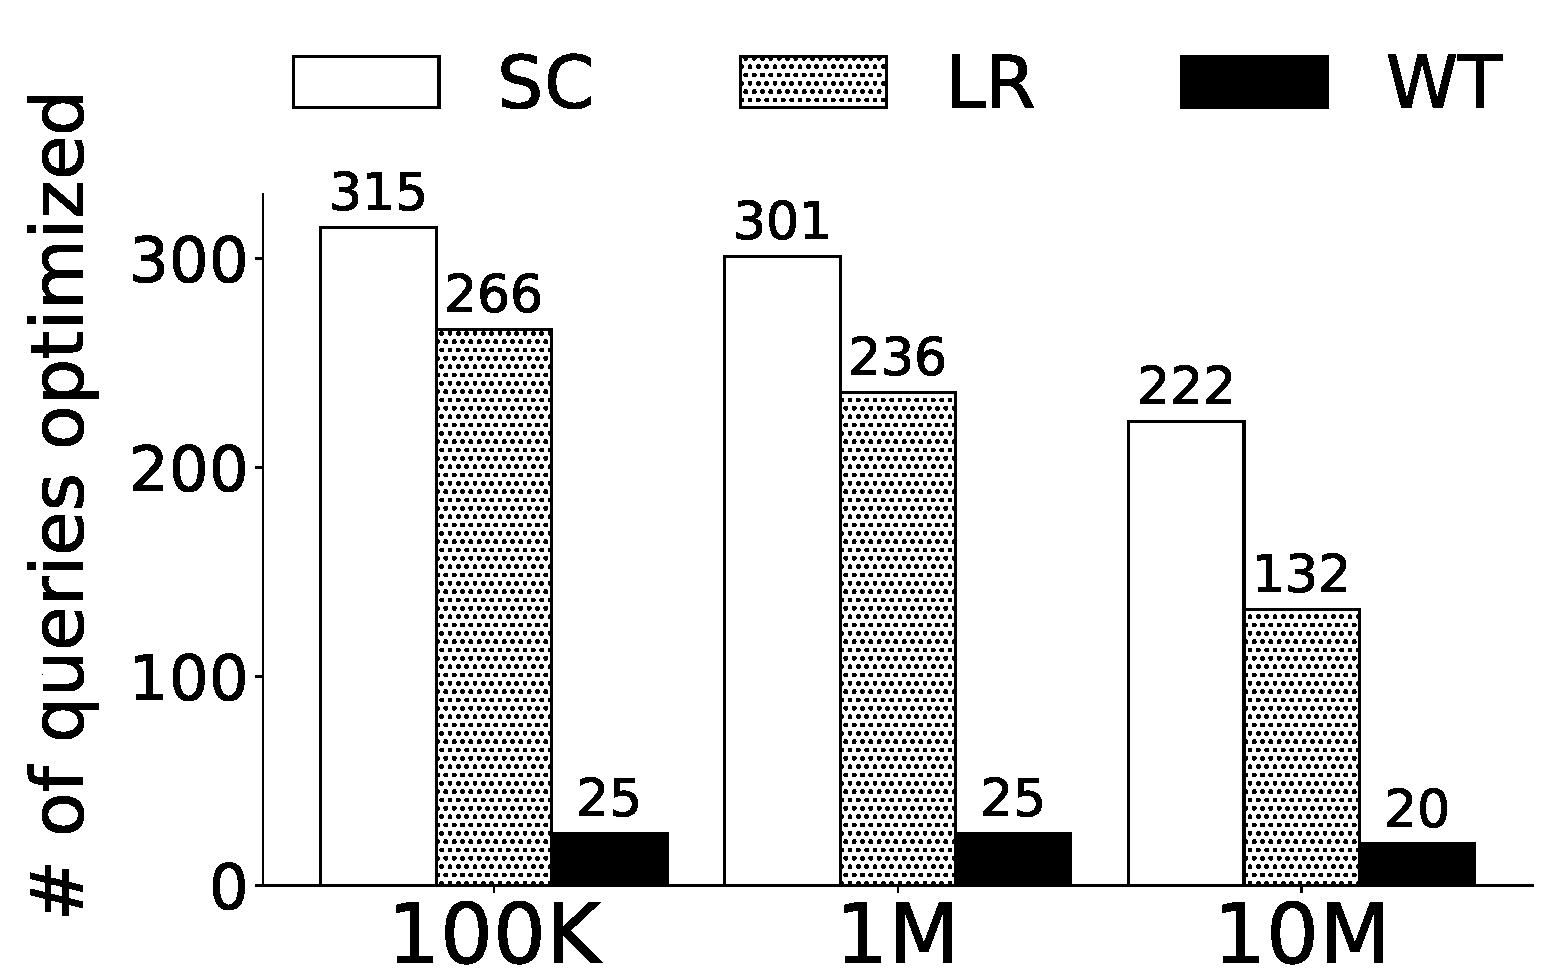
\includegraphics[width=\linewidth]{chapters/slabcity/figs/coverage_LeetCode_time.pdf}
\caption*{\small (a) Coverage (\# of queries).}
\label{slab:fig:leetcode-coverage}
\end{minipage}\hfill
\begin{minipage}[t]{.48\linewidth}\centering
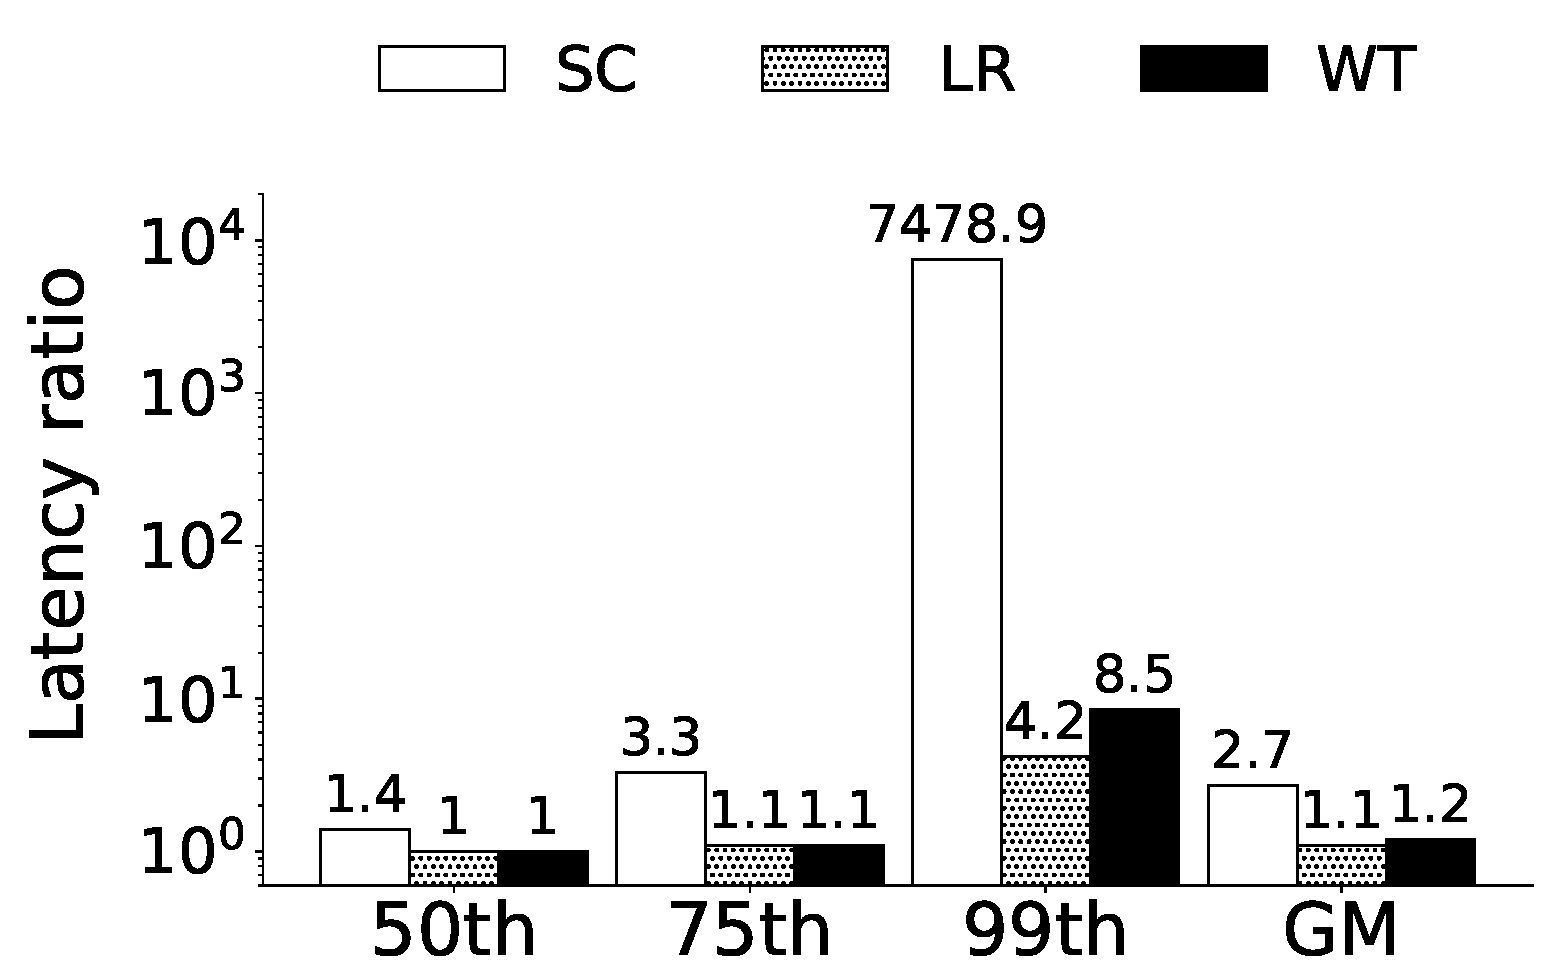
\includegraphics[width=\linewidth]{chapters/slabcity/figs/time_LeetCode_100K.pdf}
\end{minipage}\\[8pt]
\begin{minipage}[t]{.48\linewidth}\centering
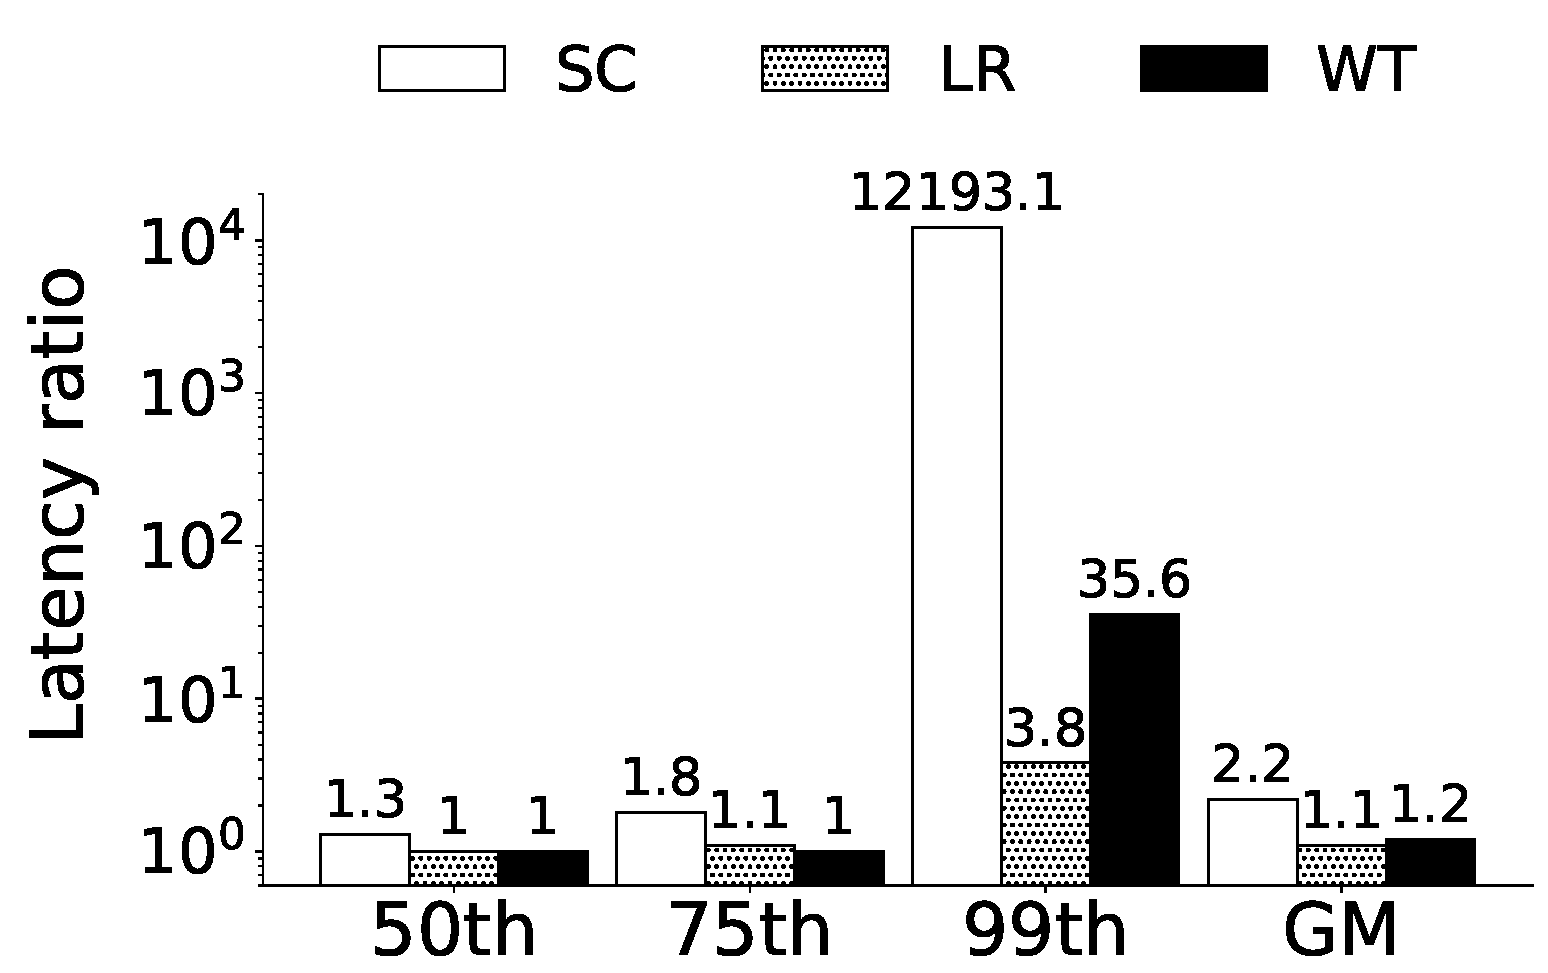
\includegraphics[width=\linewidth]{chapters/slabcity/figs/time_LeetCode_1M.pdf}
\end{minipage}\hfill
\begin{minipage}[t]{.48\linewidth}\centering
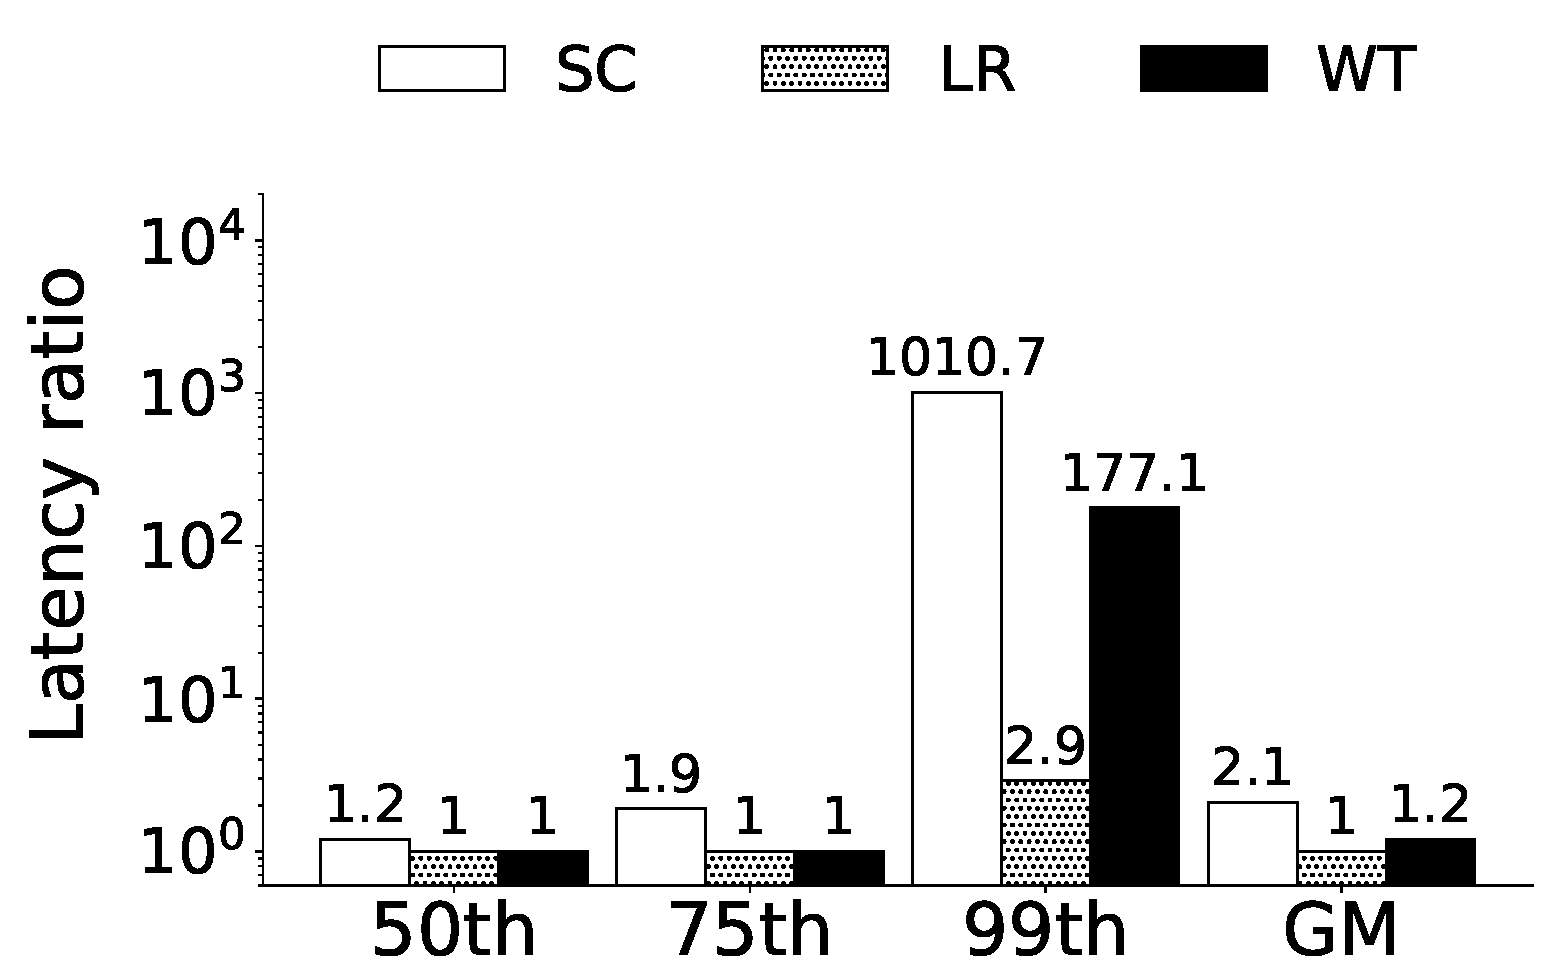
\includegraphics[width=\linewidth]{chapters/slabcity/figs/time_LeetCode_10M.pdf}
\end{minipage}
\caption*{\small (b) Latency reduction: top right is on 100K, bottom left is on 1M, and bottom right is on 10M. ``GM'' means geometric mean.}
\label{slab:fig:leetcode-reduction-latency}
\caption{\barzanrev{LeetCode results across all data sizes with uniform distribution.}}
\label{slab:fig:leetcode-results}
\end{figure*}




\begin{figure*}[!t]
\centering
% NOTE (dissertation): re-laid out from the paper's 1x4 strip to a 2x2 grid.
\begin{minipage}[t]{.48\linewidth}\centering
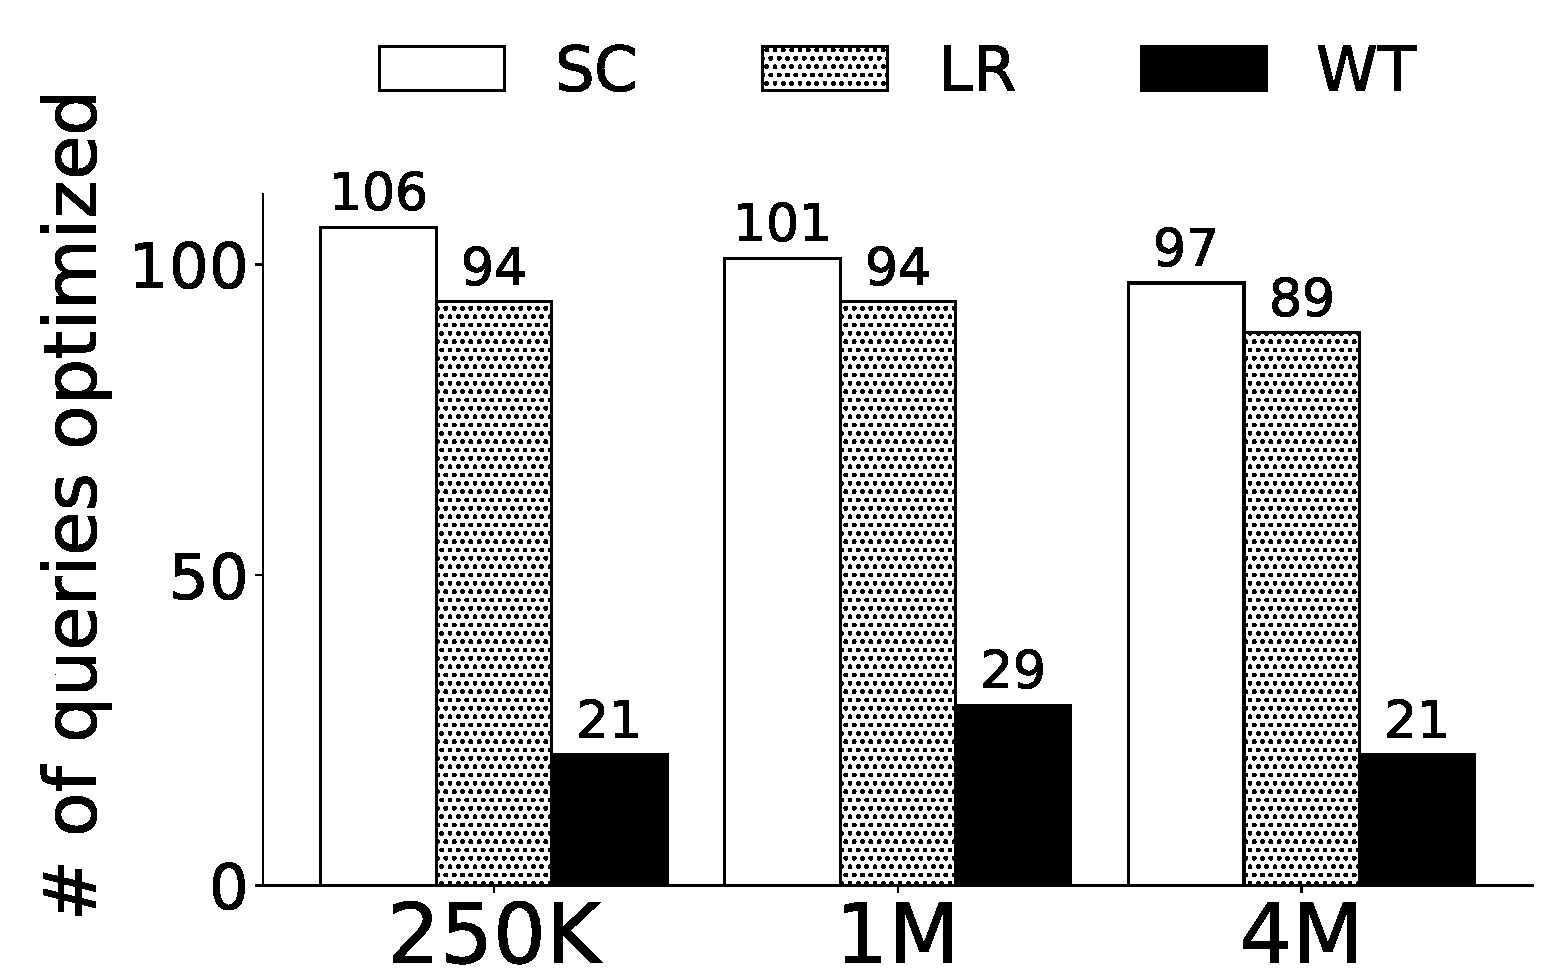
\includegraphics[width=\linewidth]{chapters/slabcity/figs/coverage_Calcite_time.pdf}
\caption*{\small (a) Coverage (\# of queries).}
\label{slab:fig:calcite-coverage}
\end{minipage}\hfill
\begin{minipage}[t]{.48\linewidth}\centering
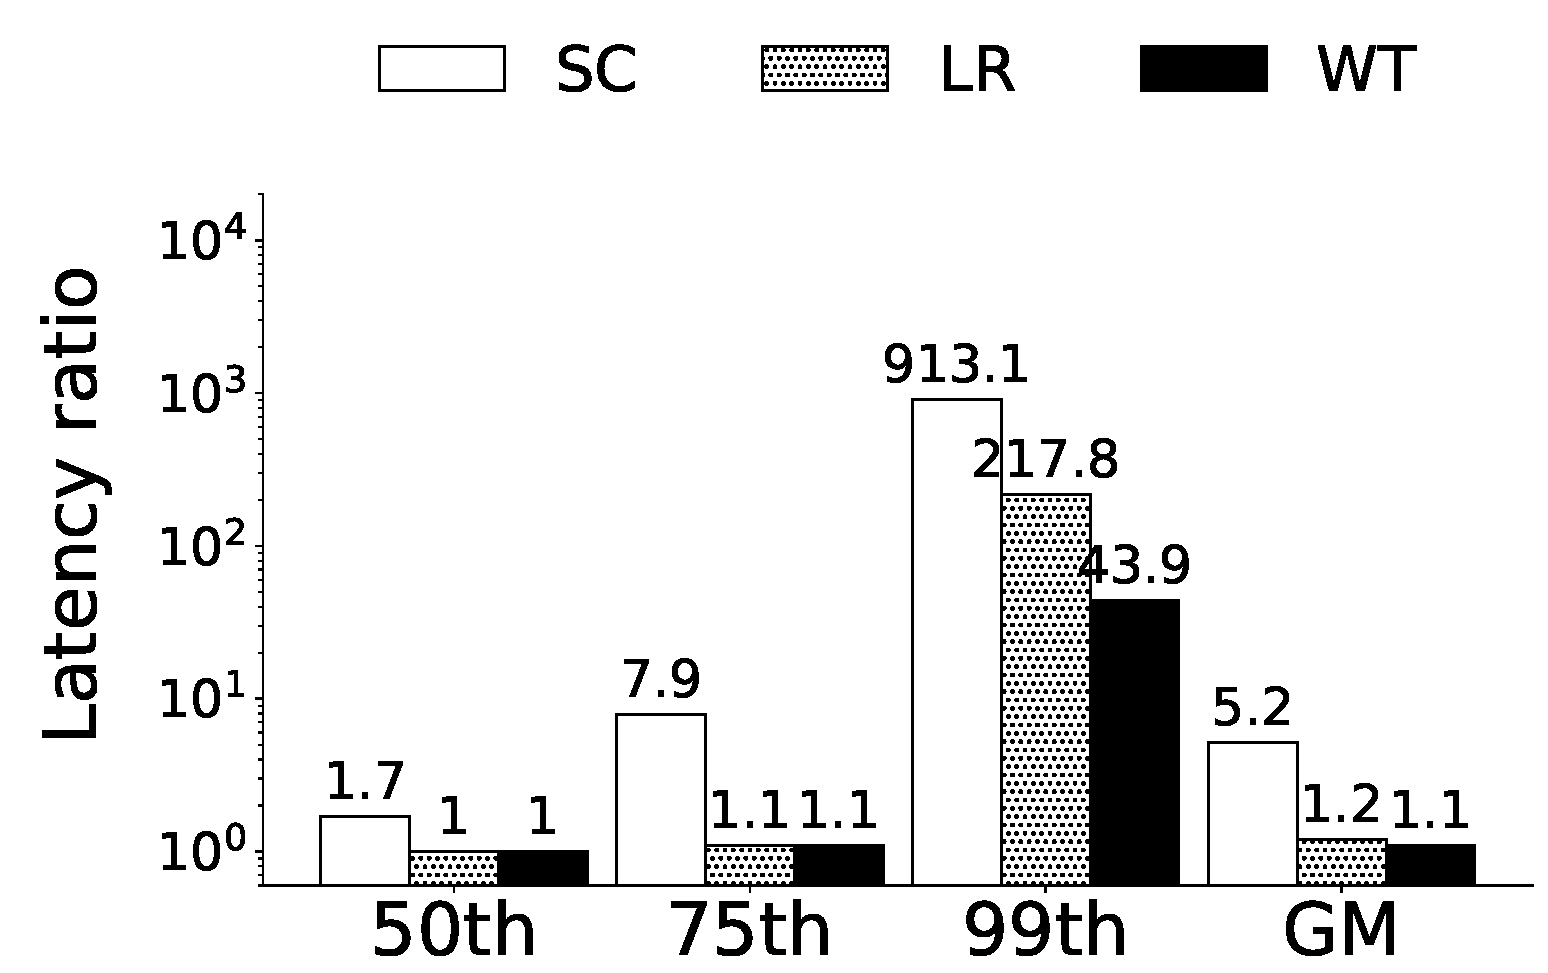
\includegraphics[width=\linewidth]{chapters/slabcity/figs/time_Calcite_250K.pdf}
\end{minipage}\\[8pt]
\begin{minipage}[t]{.48\linewidth}\centering
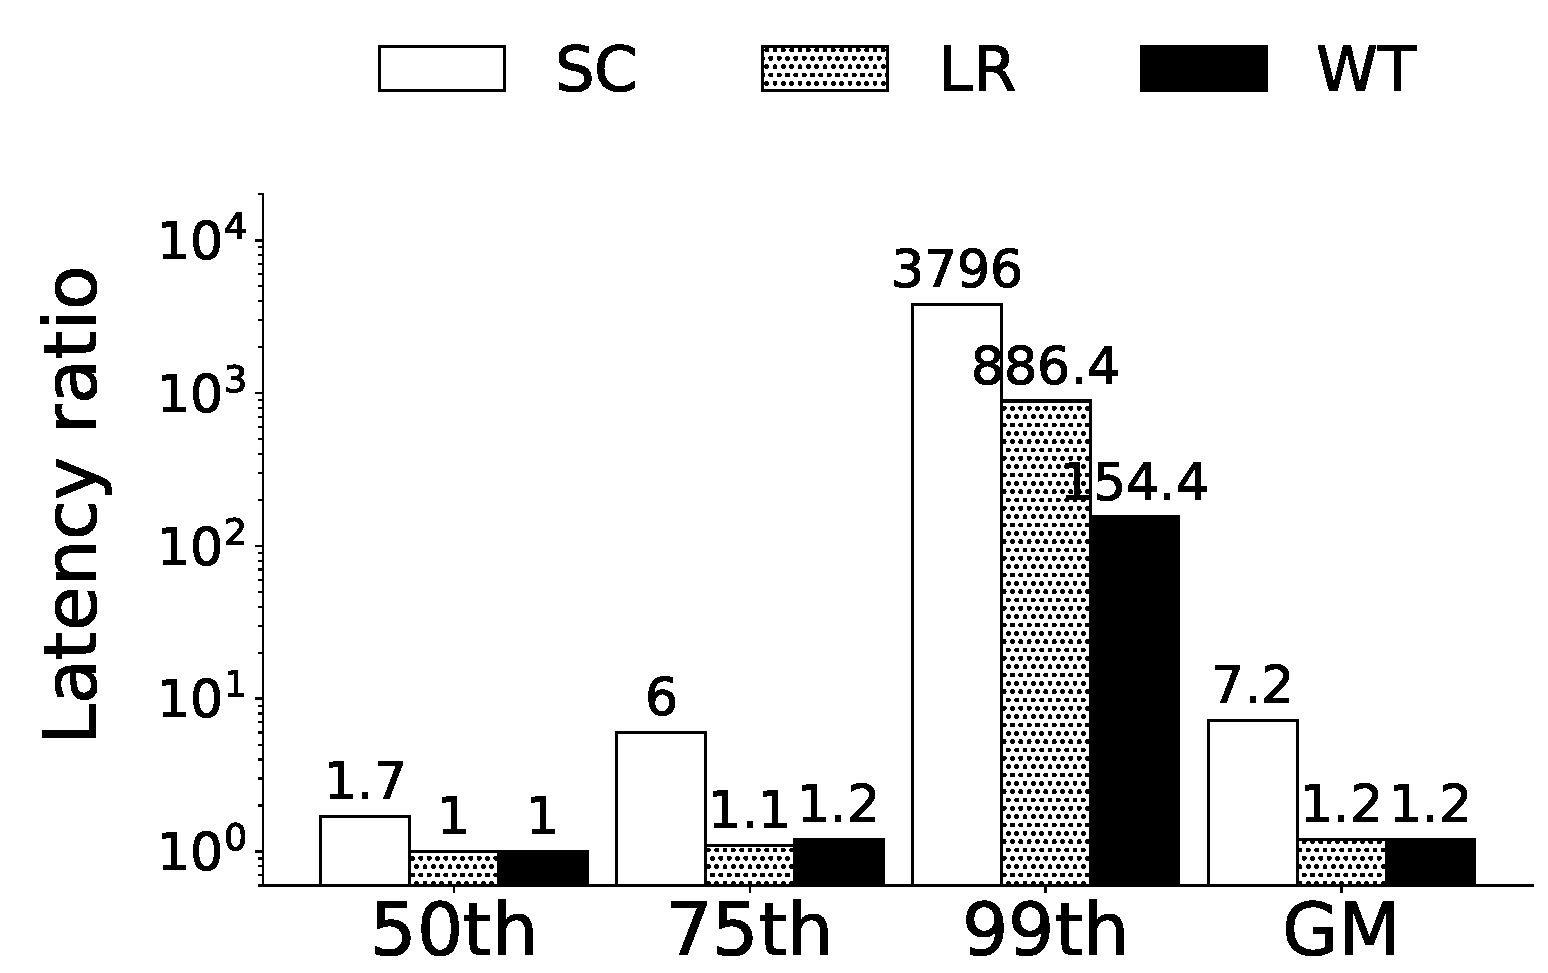
\includegraphics[width=\linewidth]{chapters/slabcity/figs/time_Calcite_1M.pdf}
\end{minipage}\hfill
\begin{minipage}[t]{.48\linewidth}\centering
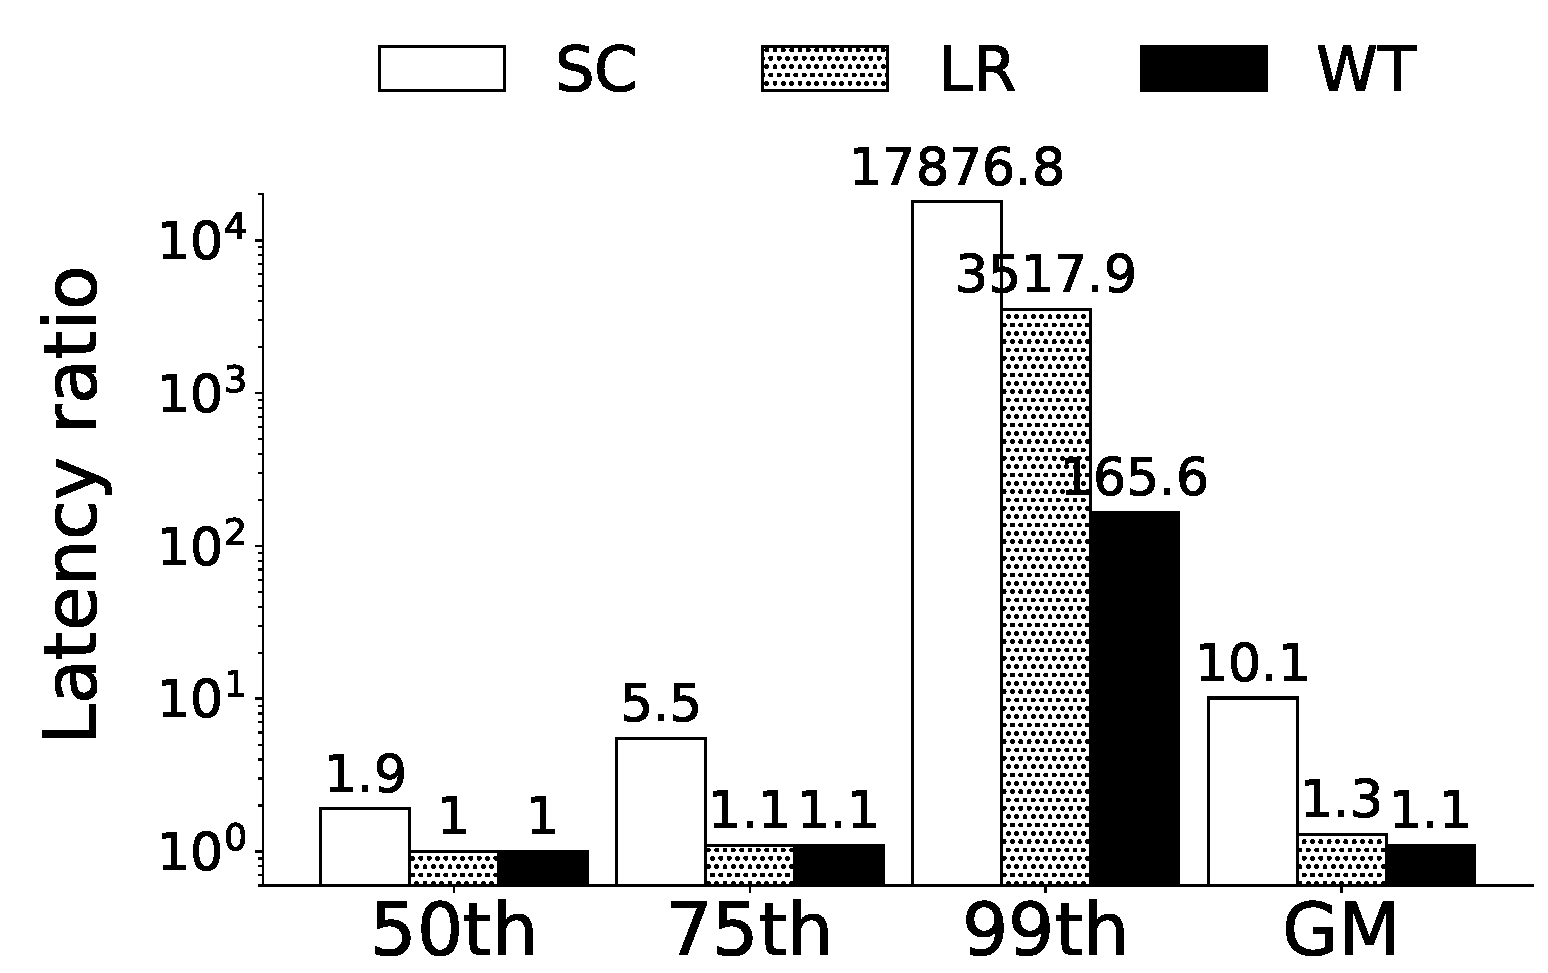
\includegraphics[width=\linewidth]{chapters/slabcity/figs/time_Calcite_4M.pdf}
\end{minipage}
\caption*{\small (b) Latency reduction: top right is on 250K, bottom left is on 1M, and bottom right is on 4M. ``GM'' means geometric mean.}
\label{slab:fig:calcite-reduction-latency}
\caption{\barzanrev{Calcite results across all data sizes with uniform distribution.}}
\label{slab:fig:calcite-results}
\end{figure*}




Our experiments are designed to answer the following questions:

\begin{itemize}[leftmargin=*]  \setlength\itemsep{2pt}
\item 
\textbf{Coverage:} 
How does $\toolname$'s \emph{coverage} compare against that of state-of-the-art query rewriting techniques? 
That is, which technique can optimize more queries? 
(Section~\ref{slab:sec:q1-coverage}) 
\item 
\textbf{Query latency reduction:}
How does $\toolname$ compare to state-of-the-art query rewriters in terms of the efficiency of the generated queries? 
That is, for input queries that can be rewritten, which technique leads to faster queries? 
(Section~\ref{slab:sec:q2-reduction})
 
\item
\textbf{Ablation study:} How important are various ideas in \slabcity? 
(Section~\ref{slab:sec:ablation})

\end{itemize}



\subsection{Experimental Setup}
%In what follows, we describe our workloads, data generation method, baselines, and experiment environment.

\head{Testbed}
All of our experiments (including running \toolname and baselines as well as executing queries) are conducted on Amazon EC2 r5.large instances,
% \barzan{is it EC2? if so then mention the size, eg. 2XL or something like that}
with 16GB RAM, 200GB gp2 SSD and Xeon E5-2686 v4 CPU running Ubuntu 22.04.
We use PostgreSQL 12.13.

\head{Workloads} 
{We use a wide range of different workloads:}
\begin{itemize}[leftmargin=*]
\item 
\textbf{LeetCode.} 
These are SQL queries, written by actual developers to solve different problems on LeetCode~\cite{leetcode}. 
Specifically, we first crawled \emph{all publicly available} SQL queries accepted by LeetCode as ``correct'' solutions. However, a number of them are actually incorrect due to missing tests on LeetCode. Hence, we manually filtered out as many incorrect queries as we could. 
In the end, we were left with a curated suite of 1131 queries overall. 
% Our dataset contains queries that solve a wide range of tasks (see some examples from Section~\ref{slab:sec:motivating-example}). 
%Then, we grouped these queries based on the LeetCode problem they are solving. 
%For each problem, we were left with dozens of correct queries that are all \emph{semantically equivalent} but \emph{syntactically distinct}.
Some of these solutions are poorly-written and therefore slow-running (which we hypothesize were authored by SQL novices) -- this makes  our LeetCode dataset especially 
valuable for evaluating query rewriting techniques. 
We also formalized the schemas and integrity constraints for all LeetCode tasks. 
%based on the description from the LeetCode website. 

\begin{comment}
\cancut{Overall, the queries were quite diverse and non-trivial. On our 10M database, \todo{xx} queries do not terminate within 10 hours, and \todo{xx} queries take at least \todo{xx} seconds to finish. Even on our smallest database with 100K rows, \todo{xx} queries take more than \todo{xx} seconds.}
\end{comment}



\item 
\textbf{Calcite.}
Our second workload is constructed from the Calcite's \emph{optimization rules} test suite~\cite{calcite-test-suite}, which is used in prior work~\cite{wetune} for evaluating query rewriting. We include all 794 queries. %in our experiments.
%The Calcite project also includes the schema and integrity constraints.


\item 
\barzanrev{\textbf{TPC.}
Finally, we also use queries from the standard TPC-H~\cite{tpc-h} and TPC-DS~\cite{tpc-ds} workloads.}
\end{itemize}


\head{Data generation} 
We generate large databases for each workload. 
For \leetcode, we use three data sizes (100K, 1M, and 10M). For \calcite, we use 250K, 1M, and 4M (4M is the largest data size that can fit in 16G memory). 
For both workloads, we follow prior work~\cite{wetune} and use \barzanrev{two different data distributions: uniform and Zipfian
% \barzan{isn't Zipfian capitalized everywhere?} \jie{also used in WeTune paper. And they also use the skewed parameter of 1.25. Do we need to mention it?}
(with a skewed parameter of 1.25, as used in \cite{wetune}).}
% \barzan{is 1.25 skeweed enough?} \jie{see above. Yes, I believe it is skewed enough}
We also make sure the generated data meets the integrity constraints. 
\barzanrev{For TPC-H and TPC-DS workloads, we use their official data generation script with the same scale factor as in $\learnedrewrite$~\cite{LR} (which is 1, meaning 1G data size).}





\head{Baselines}
We compare $\toolname$ against two state-of-the-art rule-based query rewriting techniques: 
\begin{itemize}[leftmargin=*]
\item
\textbf{\learnedrewrite} (or \LR, VLDB 2022~\cite{LR,LR-source-code}) is a state-of-the-art \emph{rule-based} query rewriter which uses Monte Carlo Tree Search to guide the rule-based rewriting process. In particular, \LR uses rewrite rules from \calcite and was shown to outperform multiple existing techniques from prior work~\cite{begoli2018apache,pirahesh1992extensible}.
\item 
\textbf{\wetune} (or \WT, SIGMOD 2022~\cite{wetune,WT-source-code}) is the state-of-the-art automated query rewrite rule generator. It had discovered dozens of new rules, previously missing from existing rule-sets. These new rules were shown to lead to new optimizations previously not considered by existing systems (such as MS SQL Server).  
\end{itemize}




\begin{comment}
\rui{All of our experiments are conducted on AWS EC2 
instances (r5.large type, with 16GB RAM, 200GB disk, Xeon E5-2686 v4 CPU, running Ubuntu 22.04 and PostgreSQL 12.13). We launched instances using the same Amazon Machine Image with testing databases loaded to ensure the same experiment setups over all instances. We collected cost by first running VACUUM ANALYZE and running EXPLAIN on queries on a single machine. For the running time, we partitioned the queries to collect their running time on multiple instances parallelly. For LeetCode experiments, we partitioned queries using problem ID so that all queries corresponding to the same problem id are run on the same instance. For Calcite experiments, we ensured that outputs that correspond to the same test were run on the same instances.  Between each run, we restarted the PostgreSQL service and cleared the cache.}
\end{comment}





%ta inja

\subsection{Coverage}
\label{slab:sec:q1-coverage}

This section reports the number of queries from each workload that \toolname can optimize, and compare it with baselines.


\head{Setup}
Given each query $\inputquery$ (and the corresponding schema) from each workload, we run \toolname (using a 5-second timeout) and obtain an output query $\query$. 
Then, we check whether or not $\query$ indeed optimizes $\inputquery$ in terms of latency: if $\query$ has a smaller latency than $\inputquery$, we say $\query$ optimizes $\inputquery$. 
%\barzan{this def should  come much earlier in the paper} %\xinyu{I added this to section 2.}
%Similarly, $\query$ optimizes $\inputquery$ in terms of latency, if $\query$ has a smaller execution time than $\inputquery$. 
We run each query (both input and rewritten queries) 3 times and take their average as the final latency value.
%the first run serves as warm-up whereas the average of the next 3 runs is used as the final latency value. 
Before each run, we restart the PostgreSQL service and clear the database cache. 
We use 10 hours as the timeout; output queries that do not terminate before timeout are marked as ``not optimized''. 
The same setup is used for the baselines. 

\vspace{5pt}
\evalfinding{\emph{\toolname can optimize more queries across different workloads.}}




\begin{table}[!t]
%\small 
\footnotesize
\caption{\barzanrev{\small LeetCode and Calcite results with Zipfian distribution.}}
\vspace{-8pt}
\centering
\setlength{\tabcolsep}{2pt}
\def\arraystretch{1.1}
\begin{tabular}{  c | r r r | r r r | r r r | r r r }
\toprule
& \multicolumn{6}{c|}{Coverage (\# of queries)} 
& \multicolumn{6}{c}{Latency ratio (geometric mean)} 
\\ 
\midrule
& \multicolumn{3}{c|}{LeetCode} 
& \multicolumn{3}{c|}{Calcite} 
& \multicolumn{3}{c|}{LeetCode} 
& \multicolumn{3}{c}{Calcite} 
\\ 
& 100K & 1M & 10M 
& 250K & 1M & 4M 
& 100K & 1M & 10M 
& 250K & 1M & 4M 
\\ 
\midrule
$\toolname$
& \textbf{318} & \textbf{269} & \textbf{186}
& {\textbf{101}} & {\textbf{99}} & {\textbf{96}}
& \textbf{3.1x} & \textbf{2.7x} & \textbf{2.2x}
& {\textbf{5.4x}} & {\textbf{8.8x}} & {\textbf{12.8x}}
\\ 
$\LR$
& 262 & 243 & 154  
& {95} & {94} & {86} 
& 1.1x & 1.2x & 1x
& {1.2x} & {1.3x} & {1.3x}

\\ 
$\WT$
& 24 & 23 & 24  
& {20} & {23} & {18}
& 1.4x & 1.6x & 1.6x
& {1.2x} & {1.2x} & {1.2x}
\\ 
\bottomrule
\end{tabular}
%\vspace{5pt}

\label{slab:tab:zipfian-results}
\vspace{-15pt}
\end{table}




\head{Results}
Figure~\ref{slab:fig:leetcode-results}(a) and Figure~\ref{slab:fig:calcite-results}(a) present the coverage results for all techinques (including $\toolname$ and baselines) across LeetCode and Calcite workloads (using a uniform distribution). 
For example, looking at Figure~\ref{slab:fig:leetcode-results}(a), for 10M, \toolname can optimize 222 input queries, whereas $\learnedrewrite$ and $\wetune$ can only 
optimize 132 and 20 queries, respectively. 
\barzanrev{We also note that since $\toolname$'s checker can fully verify only a subset of its output queries, we manually inspected all the remaining queries that only pass the tester and bounded verifier (see Section~\ref{slab:sec:eval:discussion} for a detailed discussion on the limitation of full verification) and confirmed the optimizations included in our results are indeed correct} (i.e., all input-output query pairs are equivalent).
%\barzanrev{Although the checker can offer full verification for only a subset of the output queries, we manually inspect and confirm all our optimizations are indeed correct} (i.e., all input-output query pairs are equivalent). 
\barzanrev{For the Zipfian distribution, we obtain similar results, as shown in Table~\ref{slab:tab:zipfian-results}.}
Overall, $\toolname$ significantly outperforms existing rule-based systems, highlighting the superiority of a whole-query synthesis-based approach.


\barzanrev{For the TPC-H workload, $\toolname$ is able to optimize 2 (out of 22) input queries (\#17 and \#20) in less than 5 seconds. $\LR$ is able to optimize the same two queries, while $\WT$ cannot optimize any.
The TPC-DS queries are far more complex, but $\toolname$ can still optimize three queries (\#1, \#30 and \#81) within 5 seconds. $\LR$ can optimize two (\#1, \#30) but $\LR$'s output queries are much slower than $\toolname$'s. Again, $\WT$ is not able to optimize any.}



\head{Discussion}
The gap between \toolname's coverage and baselines' on LeetCode is much higher than that on Calcite: we believe this highlights the usefulness of our LeetCode dataset and the advantage of our synthesis-based technique over rule-based ones in optimizing new query patterns. 
In particular, LeetCode has more queries that are larger and use more aggregation and window functions than those in Calcite. 
\barzanrev{While $\toolname$'s coverage is considerably higher than all baselines, there are still 
some queries covered by baselines and not covered by $\toolname$.
%While rare (\todo{??\% for)}, 
Some of these queries involve operators (e.g., coalesce) that are not yet supported by our prototype. 
Another reason has to do with our 5s timeout. 
Our plan for future improvement of our prototype (e.g., supporting more operators and optimizing the performance such as by parallelizing the search) should help with both reasons.}
%Another reason is our 5s timeout. 
%Our plans for future improvement of our implementation (supporting more operators and improving the efficiency) should help with both reasons.}





\begin{comment}
    

\todo{if above looks good, we can comment out below. }
\jierevision{There are two primary explanations as to why our tool may be unable to optimize for certain queries, while baselines can. The first reason is that baselines rewrite the input query by employing operators (e.g., $\sqlcoalescecolor$) that are not available in our DSL. The second reason is that sometimes our score function fails to capture the similarity in semantics of different dataflows and hence assigns some promising candidates with lower scores than expected. As a result, they cannot be found within 5s timeout. Table~\ref{slab:tab:Q11-Q12} shows queries finding the team size of each employee. \slabcity did not capture the relationship between $\sqloncolor \ e1.team = e2.team$ and $\sqlgroupbycolor \ team$ and failed to find the optimal query. To address this issue, one solution is to adjust the score function to take this relationship into account. However, it is important to note that incorporating more dataflows will inevitably lead to increased search time, which is a tradeoff that needs to be carefully balanced.} 

\begin{table}[!t]
\small 
\begin{tabular}{|c|c|}
\hline
 $\query_{11}$

 & 
  % \\
  %             \hspace{2em} 
 \makecell[l]{\sqlselectcolor \  e1.employee\_id, \sqlcountcolor(e2.employee\_id) \sqlascolor s\\
              \sqlfromcolor employee \sqlascolor e1 \sqljoincolor employee \sqlascolor e2 \sqloncolor e1.team = e2.team\\
              $\sqlgroupbycolor$ e1.employee\_id
              }  
\\
\hline
$\query_{12}$
&
 \makecell[l]{ \sqlselectcolor e1.employee\_id, e2.s, \\ \sqlfromcolor employee \sqlascolor e1 \sqljoincolor \\
 \hspace{0.5em} (\sqlselectcolor team, \sqlcountcolor(*) \sqlascolor s \sqlfromcolor employee \sqlgroupbycolor \ team) \sqlascolor e2 \\ \hspace{0.5em} \sqloncolor e1.team = e2.team}
 
  \\
 \hline
\end{tabular}
\vspace{5pt}
\caption{\jierevision{$\query_{11}$ is human-written. $\query_{12}$ is the optimal form.}}
\vspace{-20pt}
\label{slab:tab:Q11-Q12}
\end{table}

\end{comment}


\subsection{Query Latency Reduction}
\label{slab:sec:q2-reduction}


In this section, we compare the performance of queries synthesized by $\toolname$  with those generated by (rule-based) baselines. Higher coverage (Section~\ref{slab:sec:q1-coverage}) means $\slabcity$ can optimize more queries, 
but does it also lead to better (i.e., faster) queries than baselines?

\head{Setup}
We use the same setup as in Section~\ref{slab:sec:q1-coverage} and measure the reduction ratio in query latencies across each technique's output queries. 
For example, given $\inputquery$ and its corresponding output query $\query$ synthesized by \toolname, a latency reduction of 5x means $\query$ is 5x faster than $\inputquery$. 
We still use 10 hours as the timeout --- in case of a timeout, we use 10 hours as the latency; however, if both $\inputquery$ and $\query$ time out, we do not include this data point. 
%Latency reduction ratios for baselines are measured in the same way.

\vspace{5pt}
\evalfinding{\emph{\toolname generates faster queries across different workloads.}}


\head{Results}
We present the latency reduction results for LeetCode and Calcite workloads (using a uniform distribution) in Figure~\ref{slab:fig:leetcode-results}(b) and Figure~\ref{slab:fig:calcite-results}(b). 
For example, looking at Figure~\ref{slab:fig:leetcode-results}(b), for 10M (rightmost figure), on average, $\toolname$ achieves a 50.3x latency reduction ratio \emph{across all output queries}, whereas $\LR$ is 1.4x and $\WT$ is 12x. 
\barzanrev{We also report additional statistics: median (50th) and 75th percentiles.}
As we can see, $\toolname$ always outperforms baselines by a significant margin across both workloads and for all data sizes. 
\barzanrev{For output queries that can be covered (i.e., optimized) by $\toolname$,} the median is as high as 1.9x for LeetCode and 2.2x for Calcite.
% \barzan{what does it mean for median to be up to? shouldn't median be a single number?
% maybe we can reword to `as high as` instead of up to}
% \xinyu{because we have multiple data sizes.}
% \barzan{the following is confusing: we say on the other hand if we said on the one hand earlier which we didn't early. what are we trying to say in the next sentence? } \xinyu{we can remove OTOH}
% On the other hand, 
\barzanrev{For the Zipfian distribution, $\toolname$ also outperforms all baselines; see Table~\ref{slab:tab:zipfian-results} for more details.}

\barzanrev{For TPC-H, $\toolname$ and $\LR$ achieve similar latency speed-ups (both by more than an order of magnitude). 
For TPC-DS, $\toolname$ can optimize one query that $\LR$ is not able to optimize. For the two TPC-DS queries that both can optimize, $\toolname$ outputs faster queries compared to $\LR$'s. For all three TPC-DS queries, $\toolname$ can speed-up the original queries by at least one order of magnitude.}

%\xinyurevision{\todo{For TPC-H, $\toolname$ and $\LR$ produce queries with very similar latency reduction ratios. However, for TPC-DS, $\toolname$'s output queries are significantly faster. In particular, it achieves a {1034x} reduction for query \#1 and $\LR$ is {189x}. For \#30, $\toolname$ is {113x} and $\LR$ is {26x}. \ruirevision{For \#81, $\toolname$ is 364x and $\LR$ can not optimize.}}}


{\head{Discussion}
Similar to Section~\ref{slab:sec:q1-coverage}, \toolname's margins of improvement on LeetCode are even more significant than on Calcite, which we believe is due to the same reasons mentioned earlier: 
existing rule-based systems and \learnedrewrite's rule-set are specifically designed based on Calcite queries and LeetCode is a useful dataset to evaluate query rewriters. 
Careful readers may observe that \toolname's reduction on LeetCode 10M is lower than that on 1M.
This is due to 15 input queries (all from problem \#1308) which do not terminate within 10 hours on both sizes. Surprisingly, \toolname is able to optimize these queries: the fastest output query terminates in 3 seconds on 1M but takes more than 30 seconds on 10M. 
As we used 10 hours as the latency for the timed-out input query in both cases, this makes the reduction on 10M lower than that on 1M.}




\begin{table}[!t]
%\small 
\footnotesize
\caption{\small Time breakdown on average and other statistics.}%Bottom:  other statistics (e.g., the average number of queries enumerated).}
\vspace{-8pt}
\centering
\setlength{\tabcolsep}{3pt}
\def\arraystretch{1.5}
\begin{tabular}{  R{180pt} | r  r   }
\toprule
\% of time spent on 
& LeetCode
& Calcite
%& TPC-H 
%& TPC-DS 
\\ \midrule
{query search (line~\ref{slab:alg:toplevelalg:forloop})} 
& {37.4\%}
& {6.9\%} 
%& \ruirevision{48.0\%}
\\ 
{checking against counterexamples (line~\ref{slab:alg:toplevelalg:satisfycounterexample}}) 
& {10.8\%}
& {0.9\%}
%& \ruirevision{2.9\%}
\\ 
{equivalence  checking (line~\ref{slab:alg:toplevelalg:checkequiv}})
& {51.4\%}
& {92.2\%}  
%& \ruirevision{51.0\%}
\\ 
%\emph{\% of time on testing} 
%& 32.6\% 
%& 65.5\% 
%\\ 
%\emph{\% of time on verification} 
%& 23.6\% 
%& 31.6\% 
%\\ \midrule 
{performance ranking (line~\ref{slab:alg:toplevelalg:checkfaster})} 
& {0.4\%} 
& {0.1\%} 
%& \ruirevision{0.1\%}
\\ \midrule \midrule 
{avg \# of queries enumerated}
& {437} 
& {104}
%& \ruirevision{216}
\\ 
{avg \# of counterexamples generated}
& {1.4}
& {1.2}
%& \ruirevision{1}
\\ 
{avg \# of equivalent queries synthesized}
& {66}
& {15} 
%& \ruirevision{32}
\\ \bottomrule
\end{tabular}

\vspace{-12pt}
\label{slab:tab:time-breakdown}
\end{table}




\subsection{Detailed Analysis and Ablation Study}
\label{slab:sec:ablation}

%In this section, we analyze the time that is spent on different steps of \slabcity. We also perform a few ablation studies to measure the impact of various design decisions we have made in \slabcity.


\begin{comment}
    

\begin{table}[!t]
%\small 
\footnotesize
\centering
\setlength{\tabcolsep}{2pt}
\def\arraystretch{1.1}
\begin{tabular}{  c | r r | r r  }
\toprule
& \multicolumn{2}{c|}{LeetCode} 
& \multicolumn{2}{c}{Calcite} 
%& \multicolumn{2}{c|}{TPC-H} 
%& \multicolumn{2}{c}{TPC-DS} 
\\ 
& median 
& max 
& median 
& max 
%& median 
%& max 
%& median 
%& max 
\\ 
\midrule
$\toolname$
& {0.84} & {4.84} & 
 {0.74}	&  {4.81}	
 %& \ruirevisiontbd{4.15}  &  \ruirevisiontbd{4.58}	 &  \ruirevisiontbd{5.03}		& \ruirevisiontbd{5.74}
\\ 
$\learnedrewrite$
& 0.03 & 0.73 & 0.25	& 3.75	 
%& 0.25 & 	1.58 & 	2.48	& 25.51 
\\ 
$\wetune$
& 0.24	& 0.46 &	0.001	& 0.17	
%& 0.36	& 0.36	& NA &	NA 
\\ 
\bottomrule
\end{tabular}
%\vspace{5pt}
\caption{{\small Running time statistics to generate rewrites (in seconds). For $\toolname$, we report the time when an output query (synthesized using 5-second timeout) is found.}}
\label{slab:tab:running-time-stats}
\vspace{-20pt}
\end{table}

\end{comment}



\begin{table}[!t]
\centering
\footnotesize
\centering
\setlength{\tabcolsep}{6pt}
\def\arraystretch{1.5}
\caption{\small Running time statistics to generate rewrites (in seconds).For $\toolname$, we report the time when an output query (synthesized using 5-second timeout) is found.}
\vspace{-5pt}
\begin{tabular}{  c | r r | r r  }
\toprule
& \multicolumn{2}{c|}{LeetCode} 
& \multicolumn{2}{c}{Calcite} 
%& \multicolumn{2}{c|}{TPC-H} 
%& \multicolumn{2}{c}{TPC-DS} 
\\ 
& median 
& max 
& median 
& max 
%& median 
%& max 
%& median 
%& max 
\\ 
\midrule
$\toolname$
& {0.84} & {4.84} & 
 {0.74}	&  {4.81}	
 %& \ruirevisiontbd{4.15}  &  \ruirevisiontbd{4.58}	 &  \ruirevisiontbd{5.03}		& \ruirevisiontbd{5.74}
\\ 
$\learnedrewrite$
& 0.03 & 0.73 & 0.25	& 3.75	 
%& 0.25 & 	1.58 & 	2.48	& 25.51 
\\ 
$\wetune$
& 0.24	& 0.46 &	0.001	& 0.17	
%& 0.36	& 0.36	& NA &	NA 
\\ 
\bottomrule
\end{tabular}

\label{slab:tab:running-time-stats}
\end{table}

\begin{table}[!t]
% 
%
\centering
\footnotesize
\centering
\setlength{\tabcolsep}{2pt}
\def\arraystretch{1.1}
\caption{{\small Coverage (\# of queries) and geometric mean of latency reduction: using \texttt{EXPLAIN} vs. using exact latencies.}}
\vspace{-5pt}
\begin{tabular}{  c | r r r | r r r | r r r | r r r }
\toprule
& \multicolumn{6}{c|}{Coverage (\# of queries)} 
& \multicolumn{6}{c}{Latency ratio (geometric mean)} 
\\ 
\cmidrule{2-13}
& \multicolumn{3}{c|}{LeetCode} 
& \multicolumn{3}{c|}{Calcite} 
& \multicolumn{3}{c|}{LeetCode} 
& \multicolumn{3}{c}{Calcite} 
\\ 
& 100K & 1M & 10M 
& 250K & 1M & 4M 
& 100K & 1M & 10M 
& 250K & 1M & 4M 
\\ 
\midrule
w/ \texttt{EXPLAIN} 
& 315 & 301 & 222  & 106 & 101 & 97 
& {2.7x} & {2.2x} & {2.1x}  & {5.2x} & {7.2x} & {10.1x} 
\\ 
w/ exact latencies 
& {401} & {373} & {351}  & {121} & {117} & {112} 
& {2.9x} & {2.6x} & {2.2x}  & {4.8x} & 6.7x & {10.4x} 
\\ 
\bottomrule
\end{tabular}

\label{slab:tab:exact-latencies}
\end{table}


\head{Time breakdown}
Table~\ref{slab:tab:time-breakdown} shows the breakdown of how much time on average \toolname spends in each component (such as search and equivalence checking) and other statistics (such as the average number of queries generated during synthesis). 
In general, query equivalence checking (including both testing and verification) takes the majority of the time. 


\barzanrev{\head{Synthesis efficiency}
While $\toolname$ uses a 5s \emph{timeout}, many of its output queries are discovered 
much earlier.
Specifically, {58\%} of its output queries (generated using 5s timeout) are found within {1} second. 
In the words, the actual synthesis time to find the output query is shorter. 
Table~\ref{slab:tab:running-time-stats} presents the median and max of $\toolname$'s actual synthesis time for LeetCode and Calcite queries that $\toolname$ can rewrite.
As expected, rule-based approaches are generally faster, though $\LR$'s max time on Calcite is much slower. 
For TPC-H and TPC-DS, $\toolname$ takes 4-5 seconds for all queries it can optimize.}
%\xinyurevision{In comparison, $\LR$  is significantly slower: it takes up to 25 seconds for TPC-DS.}}














\begin{comment}

===== 
\xinyu{below is old stuff, but once we have Table 6 filled, will move something from below to above..}

As we can see, query testing takes more than 60\% of the total time, while verification takes more than 30\%. 
Note that this is not because our tester is slower than the verifier, but rather because the tester is run before verifier and disproved many inequivalent queries before they were sent to the verifier. 
For instance, on LeetCode 10M, an average of \rui{do you mean counter examples can not reject?} queries were sent to our tester, out of which only a dozen \rui{14.22} of queries were not disproved. 
On the other hand, our query search component tends to be quite fast. In particular, for LeetCode 10M, on average, a total of \rui{93 our algorithm ensures these queries are syntactically different and grammarly correct, so the number here is small, but high quality} queries can be searched within the 5-second time limit. Using \texttt{EXPLAIN} to collect cost estimates takes no time, since eventually only a handful of equivalent queries were synthesized --- e.g., for LeetCode 10M, on average, \rui{13.59} queries were ranked. 
\end{comment}



\begin{comment}


\begin{table}[!t]
\small 
\centering
\setlength{\tabcolsep}{3pt}
\def\arraystretch{1.2}
\begin{tabular}{ | r | c c c | c c c | }
\hline 
& \multicolumn{3}{c|}{LeetCode} 
& \multicolumn{3}{c|}{Calcite} 
\\ 
& 100K & 1M & 10M 
& 250K & 1M & 4M 
\\ \hline 
\emph{Query Search}
& 5.3\% & 5.4\% & 5.2\% & 0.7\% & 0.9\% & 0.9\%
\\ 
\emph{Equivalence Testing} 
& 61.4\% & 60.0\% & 60.3\%  & 66.1\% & 67.0\% & 67.3\%\\ 
\emph{Equivalence Verification} 
& 33.0\% & 34.3\% & 34.2\%  & 33.0\% & 32.0\% & 31.7\%\\ 
\emph{Performance Ranking} 
& 0.3\% & 0.3\% & 0.3\%  & 0.1\% & 0.1\% & 0.1\%
\\ \hline 
\end{tabular}
\vspace{5pt}
\caption{$\toolname$ time breakdown.}
\label{slab:tab:time-breakdown}
\end{table}

\end{comment}


\head{Impact of CEGIS}
How beneficial is the use of CEGIS? That is, if we do not re-use counterexamples when disproving queries, how inefficient would \toolname become? 
%In general, program synthesis is known to be prohibitively slow without using counterexamples~\cite{solar2008program}. To validate this in the context of synthesis-based query rewriting, 
%For instance, 
For LeetCode, with CEGIS, on average, $\toolname$ can search {437} queries in 5 seconds, where {1.4} counterexamples are generated; however, without re-using these examples, it can only search 175 queries on average within the same amount of time. 
This is because the tester spends extra time generating new counterexamples which are later dropped, but clearly they can be re-used to disprove other queries.  
This validates the observation made in prior work that CEGIS helps boost efficiency~\cite{solar2008program}. 

%generate \tofix{the examples from scratch.}\barzan{can we instead say `to disprove the same queries'?}
%This validates the observation made in other domains that CEGIS is critical for synthesis efficiency~\cite{solar2008program}. 




\head{Impact of query testing}
It is critical to reduce the frequency of invoking query verification. 
For instance, for LeetCode, on average our tester can disprove several dozens of queries within 1 second, whereas the verifier typically can handle at most a couple of queries within the same amount of time.
%A variant of \slabcity that invokes the query verifier to disprove \emph{every} candidate query (rather than always running the tester first)


\head{Impact of using dataflows to guide search}
A variant of $\slabcity$ that uses a naive search algorithm (that enumerates queries based on query size) was not able to optimize any of our input queries within 5 seconds. 
This highlights the importance of using dataflows to significantly accelerate query synthesis. 

\head{Impact of using cost estimates for ranking}
\texttt{EXPLAIN} is known to give inaccurate cost estimates. 
We study a variant of \slabcity where, instead of \texttt{EXPLAIN}, we  use the actual latency for each query (by running it against the database). 
While this variant is clearly impractical, it helps us understand how much \slabcity could be improved if we had access to a perfect predictor that could give the exact latency values. 
Table~\ref{slab:tab:exact-latencies} compares $\toolname$ w/ exact latency against our current $\toolname$ w/ \texttt{EXPLAIN} in terms of coverage; Table~\ref{slab:tab:exact-latencies} compares them in terms of latency reduction. 
In general, using exact latencies yields slightly higher coverage and latency reduction ratios, which is expected as that is the perfect predictor. 
However, we notice that using \texttt{EXPLAIN} to estimate query latency gives very close results and we believe this is a reasonable trade-off. 



\begin{comment}
    

\begin{table}[!t]
\footnotesize
\centering
\setlength{\tabcolsep}{3pt}
\def\arraystretch{1.1}
\begin{tabular}{  c | rrr | rrr  }
\toprule
& \multicolumn{3}{c|}{LeetCode} 
& \multicolumn{3}{c}{Calcite} 
%& \multirow{2}{*}{\rotatebox{0}{TPC-H}}
%& \multirow{2}{*}{\rotatebox{0}{TPC-DS}} 
\\ 
& 100K & 1M & 10M 
& 250K & 1M & 4M 
%& & 
\\ \midrule
w/ \texttt{EXPLAIN} 
& 315 & 301 & 222  & 106 & 101 & 97 
%& \ruirevision{2}  & \ruirevision{2}
\\ 
w/ exact latencies 
& {401} & {373} & {351}  & {121} & {117} & {112} 
%& \ruirevision{2}  & \ruirevision{2}
\\ \hline 
\end{tabular}
\vspace{5pt}
\caption{\small Coverage \ruirevision{(\# of queries)}: using \texttt{EXPLAIN} vs. using exact latencies.}
\label{slab:tab:oracle-coverage}
\vspace{-20pt}
\end{table}


\begin{table}[!t]
\footnotesize
\centering
\setlength{\tabcolsep}{2pt}
\def\arraystretch{1.1}
\begin{tabular}{  c | rrr | rrr }
\toprule
& \multicolumn{3}{c|}{LeetCode} 
& \multicolumn{3}{c}{Calcite} 
%& \multirow{2}{*}{\rotatebox{0}{TPC-H}}
%& \multirow{2}{*}{\rotatebox{0}{TPC-DS}}
\\ 
& 100K & 1M & 10M 
& 250K & 1M & 4M 
%& 
%& 
\\ \midrule   
w/ \texttt{EXPLAIN} 

& {2.7} & {2.2} & {2.1}  & {5.2} & {7.2} & {10.1} 
%& \ruirevision{1429.4} & \ruirevision{341.6}

\\ 
w/ exact latencies 

& {2.9} & {2.6} & {2.2}  & {4.8} & 6.7 & {10.4} 
%& \ruirevision{1429.4} & \ruirevision{341.6}

\\ \bottomrule
\end{tabular}
\vspace{5pt}
\caption{\small Geometric mean of latency reduction: using \texttt{EXPLAIN} vs. using exact latencies.}
\label{slab:tab:oracle-reduction1}
\vspace{-20pt}
\end{table}

\end{comment}



\head{Percentage of fully verified rewrites}
A subset of $\slabcity$'s rewrites can be \emph{fully} verified by the {full} verifier --- meaning queries in this subset are guaranteed to be equivalent to their corresponding input queries, \emph{for all possible inputs}.
For example, for LeetCode 100K, {17\%} of the queries can be fully verified by $\cosette$ and $\spes$. We explain the implications in the next Section~\ref{slab:sec:eval:discussion}.


\subsection{Discussion}
\label{slab:sec:eval:discussion}


\barzanrev{While $\toolname$'s percentage of fully verified rewrites (about 17\%) might sound low, one 
must remember that the vast majority of rewrite rules in existing rule-based techniques are not fully verified~\cite{chu2017hottsql,chu2018axiomatic} and rely on human verification, which is error-prone. In fact, a considerable fraction (about 5\%) of rewrites generated by $\learnedrewrite$ using the Calcite rule-set were proved  incorrect by $\toolname$'s checker. %Further inspection also revealed multiple buggy rewrite rules (confirmed by Calcite developers~\cite{calcite-bug-1,calcite-bug-2,calcite-bug-3}). 
In contrast, all of $\toolname$'s rewrites pass the checker. 
Even those few prior approaches that do offer formal guarantees, they do so for a much smaller 
%percentage
{number}
of queries than $\toolname$ (e.g., 7 queries in the FGH work~\cite{wang2022optimizing}). 
%vs. \xinyurevision{more than 50 in $\toolname$}). 

In reality, the percentage of rewrites that can benefit from full verification has little impact on $\toolname$'s specific use case, which, as explained in Section~\ref{slab:sec:intro}, is any scenario where a query is rerun many times, such as BI dashboard queries. 
In such scenarios,  many rewrites receiving a ``bounded verification'' flag is not a hindrance since the human inspection can be performed at the time of defining the queries and before deploying the dashboard to production.}

\barzanrev{Furthermore, $\toolname$'s use of a tester and a bounded verifier in conjunction with full verification offers two key improvements. 
First, they can very effectively eliminate incorrect rewrites (by more than 80\%) and hence allow human experts to focus their effort on inspecting a much smaller set of high-quality rewrites. For example, as mentioned earlier, our checker proves 5\% of $\LR$'s rewrites to be wrong. 
Second, rewrites that pass our tester and bounded verifier are highly likely to be correct: among $\toolname$'s rewrites that pass, 97\% of them are confirmed to be correct (either via full verification or manual inspection) and only 3\% are found to be incorrect.}

\barzanrev{Finally, $\toolname$ is an important step in the right direction: there are many use cases that are not covered by state-of-the-art techniques, and $\toolname$ can discover non-trivial whole-query optimizations for many of those cases.  
$\toolname$ can also be used to augment existing approaches, whereby 
one can still rely on rule-based rewriting when applicable and invoke $\toolname$ otherwise.}


%\barzanrev{In fact, $\toolname$'s use of an automated tester and a bounded verifier in conjunction with full verification is a major improvement: (1) queries that are fully verified need no human inspection at all, and more importantly (2) our tester and bounded verifier can eliminate incorrect rewrites (by more than 80\%). This allows the human experts to focus their effort on inspecting a much smaller subset of high-quality rewrites. In contrast, existing techniques immediately resort to manual inspection when the (limited) full verification fails.}

%\barzanrev{We also note that the tester and bounded verifier in $\toolname$ are very effective in practice: it is quite rare for an incorrect query to pass our checker. As mentioned earlier, the checker proves 5\% of $\learnedrewrite$'s rewritten queries to be wrong and reveals multiple buggy rewrite rules from Calcite. For $\toolname$'s rewrites that pass its tester and bounded verifier, 97\% of them are confirmed to be correct (either via full verification or manual inspection) and only 3\% are found to be incorrect.}

\begin{comment}

Finally, \xinyu{yet to write this part, but this part is easy.}

\jie{Version 1: full - bounded - human inspection}

\jierevision{\head{Limited full verification and its implications}
SlabCity's full verification coverage of 17\% may initially seem low, but it is crucial to consider the limited verifiability of rules employed by existing approaches, which heavily rely on error-prone human verification. Our bounded verifier uncovered incorrect rewrites in prior work, revealing the shortcomings of relying solely on human verification. In contrast, all of SlabCity's rewrites successfully passed our tester and bounded verifier. Being able to uncover faulty rewrites of rule-based approaches also demonstrates effectiveness of our bounded verifier, which enables users to focus their manual inspection on a small set of high-quality rewrites. For a rewrite to pass our bounded verification, it is very difficult and thus extremely valuable. In terms of real-life applicability, the reliance on bounded verification for 83\% of the rewrites in SlabCity does not hinder its practicality. This is because SlabCity targets dashboard queries, which undergo human inspection prior to deployment in production. SlabCity fills the gap by providing a solution for queries that do not benefit from existing rules. By combining rule-based rewriting when applicable and leveraging SlabCity otherwise, users can achieve a net benefit in terms of query optimization.}

\jie{Version 2: full - human inspection - bounded}

\jierevision{\head{Limited full verification and its implications}
SlabCity's full verification coverage of 17\% may initially seem low, but it is crucial to consider the limited verifiability of rules employed by existing approaches, which heavily rely on error-prone human verification. Our bounded verifier uncovered incorrect rewrites in prior work, revealing the shortcomings of relying solely on human verification. In contrast, all of SlabCity's rewrites successfully passed our tester and bounded verifier. In terms of real-life applicability, the reliance on bounded verification for 83\% of the rewrites in SlabCity does not hinder its practicality. This is because SlabCity targets dashboard queries, which undergo human inspection prior to deployment in production. Being able to uncover faulty rewrites of rule-based approaches also demonstrates effectiveness of our bounded verifier, which enables users to focus their manual inspection on a small set of high-quality rewrites. For a rewrite to pass our bounded verification, it is very difficult and thus extremely valuable. SlabCity fills the gap by providing a solution for queries that do not benefit from existing rules. By combining rule-based rewriting when applicable and leveraging SlabCity otherwise, users can achieve a net benefit in terms of query optimization.}

\end{comment}
\section{Conclusion and Future Work}
\label{slab:sec:conc}



In this work, we presented \slabcity, the first {synthesis-based query rewriting technique that is capable of \emph{whole-query} optimization without requiring rewrite rules.} 
$\slabcity$ is not restricted to a given set of rewrite rules, and therefore is able to explore a larger space of candidate queries for more fruitful optimizations. 
In particular, our evaluation shows that, not only can \toolname  optimize many more (up to 1.7x more) queries than state-of-the-art query rewriters, but it also generates more interesting queries that are significantly faster (by up to 4 orders of magnitude). 


\barzanrev{We believe our general framework of using dataflows to synthesize rewrites is applicable to discovering rewrite rules as well akin to $\wetune$~\cite{wetune}. Specifically, given a query $\inputquery$ with an integrity constraint $\dataconstraint$, one can first use $\toolname$ to obtain a faster query $\query$. Then, this specific transformation $\inputquery \rightarrow_{\dataconstraint} \query$ can be generalized to a pattern $T_{\emph{in}} \rightarrow_{\psi} T$ where $T_{\emph{in}}$ and $T$ are query templates and $\psi$ is a more general constraint such that this more general transformation still preserves equivalence. One can leverage the verifier in $\wetune$ to check equivalence of $T_{\emph{in}}$ and $T$ under $\psi$. 
}

\barzanrev{
We also note that query rewriting is orthogonal to traditional query optimization and query tuning techniques, and thus, 
\slabcity can be leveraged alongside such techniques. 
% In fact, the manual efforts put into query tuning can be directed to optimizing the rewritten query's plan rather than the original query’s plan. This is because the former is more likely to be amenable to query tuning: 
 In general, given the same amount of time and engineering resources, it should be easier to tune a rewritten query than the original one since the query optimizer starts with a more optimal query plan than it would with a poorly expressed query. 
   In other words, the set of query plans that can be uncovered with traditional query optimization techniques is heavily limited by the starting query, which is the main reason query rewriting techniques have been a subject of much research in the field. However, a more comprehensive study to quantify the impact of better query rewriting on the effectiveness of traditional query tuning will make for an interesting future work. 
}


\begin{comment}
\xinyurevision{Finally, readers may  have noticed that our query syntax (from Figure~\ref{slab:fig:querysyntax}) does not include the logical negation operation. This is simply because in our benchmarks, it is not used as frequently as other operators, and therefore not included. However, supporting negation is quite straightforward: we only need to make a couple of changes to our implementation such as extending our parser and adding a rule to compute the dataflow for negation. Our framework would remain the same. This is also true for adding other operators. }
\end{comment}




%===================================================================
% Chapter: GenRewrite (SIGMOD 2026 / PACMMOD)
% Sections are the final paper sources, included verbatim.
% Labels are prefixed with "gen:"; the paper's \tool macro was
% renamed to \genrewrite.
%===================================================================
\chapter{GenRewrite: Query Rewriting via Large Language Models}
\label{gen:chap}

\begingroup
\renewcommand{\thefootnote}{}%
\footnotetext{The material in this chapter is adapted from published
work: Jie Liu and Barzan Mozafari, ``GenRewrite: Query Rewriting via
Large Language Models,'' \emph{Proceedings of the ACM on Management of
Data} 4(1) (SIGMOD), Article 70, 2026~\cite{genrewrite}.}%
\endgroup

\lstset{style=genrewriteCode}

\section{Introduction}\label{gen:sec:intro}

Inefficient queries are a significant problem for nearly any organization relying on a database system. These poorly written queries—whether authored by inexperienced users or auto-generated by business intelligence (BI) tools—are a major cause of slow performance and, in cloud databases like Snowflake~\cite{dageville2016snowflake} or BigQuery~\cite{fernandes2015bigquery}, can lead to excessive costs. 
As a result, SQL-to-SQL query rewriting is a crucial step in optimizing performance and reducing expenses, 
as the likelihood of the query optimizer finding an efficient query plan is significantly diminished if it is given a poorly-written query to begin with. 
However, whether performed manually or automatically, query rewriting has remained a challenging task.

\genhead{Challenges of manual query rewriting}
The poorly-written queries that have the biggest impact on the overall cost and performance tend to be quite complex too. 
For example, it is not uncommon for queries auto generated by
Looker~\cite{lookergoogle} to span 100s of lines.
Ensuring the rewritten query preserves the semantics of the original requires a deep understanding of the database schema, constraints, and the user intent, and is therefore a time-consuming and error-prone task, even for seasoned database experts.
The fact that there are often thousands, if not millions, of such slow queries makes the manual approach a monumental undertaking.

\genhead{Limitations of traditional automated query rewriting} 
Despite extensive research, automated query rewriting techniques have long faced fundamental limitations that hinder their practical effectiveness. The most common approach relies on \emph{rewrite rules}—--pattern-matching transformations that replace query fragments with optimized equivalents while preserving semantics. 
Regardless of whether the rules are developed and provided by experts~\cite{bruno2022computation,pirahesh1992extensible,ahmed2006cost} or 
are inferred automatically~\cite{wetune,ding2023proving},
a rule-based query rewriter is as effective as the set of rules provided to it. 
By definition, rule-based query rewriters\footnote{Rule-based query \emph{rewriting} should not be confused with rule-based query \emph{optimization}; the latter is simpler, and thus much more common in practice~\cite{graefe1987rule}.}
% are limited to situations where the input query matches one of their existing rules,  
% and thus
are fundamentally incapable of optimizing new query patterns that do not match their existing rules~\cite{dong2023slabcity}.
Although synthesis-based query-rewriting does not require prior rules~\cite{dong2023slabcity}, in practice it only handles simple queries---for instance, SlabCity~\cite{dong2023slabcity} optimizes just 2 out of 22 TPC-H~\cite{tpch} queries and 3 out of 99 TPC-DS~\cite{tpcds} queries.



\begin{comment}

\begin{table*}[htbp]
\centering
\label{gen:tab:plan_templates}
\begin{tabular}{|c|c|c|c|}
\hline
\textbf{No.} & \textbf{Source Query Pattern} & \textbf{Destination Query Pattern} & \textbf{Constraints} \\
\hline
1 & $\operatorname{Sel}_{\mathrm{p}, \mathrm{r} . \mathrm{a}_0}(\operatorname{Proj}_{\mathrm{r} . \mathrm{a}_1}(\mathrm{r}))$ & $\operatorname{Proj}_{\mathrm{r} . \mathrm{a}_1}(\operatorname{Sel}_{\mathrm{p}, \mathrm{r} . \mathrm{a}_0}(\mathrm{r}))$ & $\operatorname{SubAttrs}(a_0, a_1)$ \\
\hline
2 & $\operatorname{Proj}_{\mathrm{r} . \mathrm{a}_0}(\operatorname{Sel}_{\text {p,r. } \mathrm{a}_1}(\text { Proj }_{\mathrm{r} . \mathrm{a}_2}(\mathrm{r})))$ & $\operatorname{Proj}_{\mathrm{r} . \mathrm{a}_0}(\operatorname{Sel}_{\mathrm{p}, \mathrm{r} . \mathrm{a}_1}(\mathrm{r}))$ & $\operatorname{SubAttrs}(a_0, a_2), \operatorname{SubAttrs}(a_1, a_2)$ \\
\hline
3 & $\text { LJoin }_{\mathrm{r}_0, \mathrm{a}_0, \mathrm{r}_1 \cdot \mathrm{a}_1}(\mathrm{r}_0, \mathrm{r}_1)$ & $\text { IJoin }_{\mathrm{r}_0 \cdot \mathrm{a}_0, \mathrm{r}_1 \cdot \mathrm{a}_1}(\mathrm{r}_0, \mathrm{r}_1)$ & $\operatorname{RefAttrs}(\mathrm{r}_0, \mathrm{a}_0, \mathrm{r}_1, \mathrm{a}_1), \operatorname{NotNull}(\mathrm{r}_0, \mathrm{a}_0)$ \\
\hline
\end{tabular}
\caption{Examples of rewrite rules in WeTune~\cite{??}}
\end{table*}



\begin{enumerate}
    \item \textbf{Semantic side}: Ensuring that the rewrite preserves the semantics of the original query is crucial, which requires a deep understanding of the database schema, constraints, and the query intent.
    \item \textbf{Syntax side}: SQL queries and database schemas can be both highly complex. Manipulating their elements without introducing errors requires sophisticated analysis.
\end{enumerate}
\end{comment}

% \genbarzan{use either Text-to-SQL or Natural Language to SQL (NL2SQL) consistently everywhere in the paper}

% a few other 
% \genbarzan{would be better to name those areas here and cite them, e.g., blah~\cite{`}, blah~\cite{} and blah~\cite{}}
% areas~\cite{citeALlOtherPapersThatHaveAppliedLLMsToADBProblemExceptTheTextToSQLAndTheVisionPaperYouSentLastNight}, 

\genhead{Large language models (LLMs)} The shining success of large language models (LLMs) in performing complex and open-ended tasks has created new hopes for solving some of the hardest database problems as well. 
While researchers have used LLMs for Text-to-SQL~\cite{fu2023catsql,gao2023text,sun2306sql,katsogiannis2023survey,pourreza2024din} and a few other areas, e.g., data cleaning and integration~\cite{narayan2022can,suhara2022annotating}, table processing~\cite{li2023table,lu2024large} and database diagnosis~\cite{zhou2023d}, their potential for query rewriting has remained largely unexplored. In instances where human experts or existing rules cannot rewrite a query, say for complex queries or new query patterns, 
 could LLMs be leveraged to uncover rewrite opportunities due to their broad general knowledge and advanced reasoning capabilities? If so, this could drastically lower the burden on human experts and allow for a much larger set of queries to benefit from rewriting.
To the best of our knowledge, this paper is the first\footnote{See \S\ref{gen:sec:related} for related work published after the initial publication of our work on ArXiv.} to focus on 
 answering this question: how to best leverage LLMs for query rewriting beyond rules and how to address the challenges involved.

\genhead{Challenges} Using LLMs for query rewriting has challenges:\footnote{A common misunderstanding is that the time and monetary overhead of invoking an LLM may outweigh the speedup benefits of the rewrite. However, this one-time overhead is less relevant for repetitive workloads, which are the focus of \genrewrite (see \textbf{Target workloads}).} 
\begin{enumerate}[label=C\arabic*, leftmargin=0.5cm]

\item The na\"ive  approach of simply prompting the LLM to "rewrite the given query into a faster but equivalent form"  can rarely handle complex queries: 
most outputs either fail to parse (syntactic errors) or produce incorrect results (semantic errors) due to SQL’s complexity and LLM hallucinations (\S~\ref{gen:sec:expr:llmbaseline}).
%~\cite{zhang2023siren,tonmoy2024comprehensive}.

\item LLMs lack a database cost model and cannot run experiments, so their rewrites are not necessarily faster than the original queries.

\item While LLM costs for rewriting a recurrent workload can be amortized, excessive invocations can still become expensive.
     
\item Hints can help the LLM, but excessive or irrelevant ones can lead to mistakes.

\item Due to their black-box nature, LLM rewrites are harder for humans to understand and verify than traditional  rules.

\end{enumerate}

%ta inja
\genhead{Our approach}
To address the above challenges, we present \textbf{\genrewrite}, the first holistic system that leverages LLMs for query rewriting. 
We introduce the notion of a Natural Language Rewrite Rule (NLR2), which is a textual explanation summarizing the rewrite. 
We use the LLM itself to produce the NLR2s, which are then used for three purposes. The NLR2s 1)  serve as hints assisting the LLM to provide better rewrites 
(C2), requiring fewer follow-up LLM invocations (C4), 2) make the rewrites easier to understand and verify by offering a human-readable explanation (C5), and, 
most importantly, 3) allow \genrewrite to transfer the knowledge gained from rewriting one query to another and thus become smarter and more effective over time (C1, C2, C3). Since NLR2s are void of confidential information (such as column or schema names), one can even bootstrap \genrewrite's NLR2 repository for a new workload using the repository of a previously trained \genrewrite on another workload.

To avoid redundant rules, which can in turn confuse the LLM, we maintain
    a utility score for each NLR2 to supply only those rules to the LLM  as hints that are most relevant to the query at hand.
Finally, to minimize the LLM cost and minimize the human effort needed for manual verification, 
\genrewrite does not discard incorrect rewrites. Instead, it uses a novel counterexample-guided technique to iteratively
    correct the syntactic and semantic errors in the rewritten query (C1, C3).

\begin{figure}[ht]
\inv\sinv
  \centering
  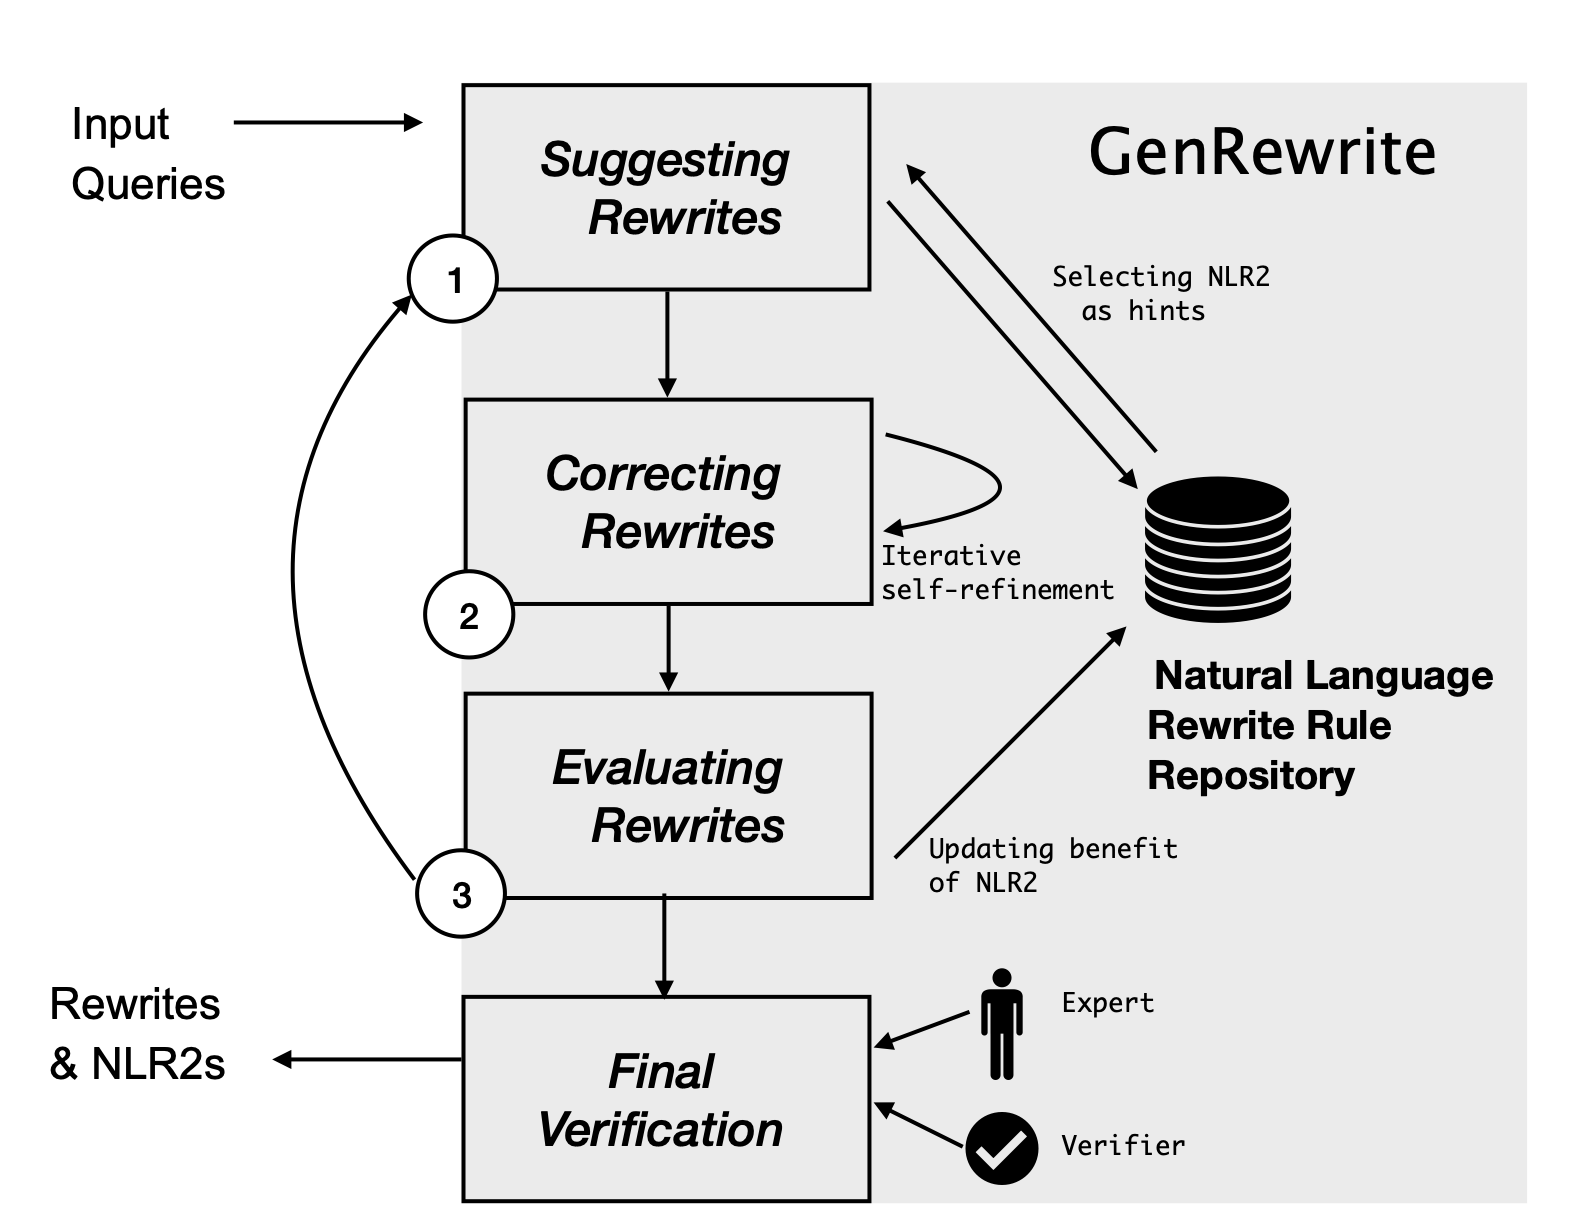
\includegraphics[width=0.8\linewidth]{chapters/genrewrite/figures/workflow.1.png}
\inv\inv
  \caption{High-level Workflow of \genrewrite }
  \label{gen:fig:arch}
\inv
\end{figure}

% \genbarzan{don't forget to fix the plot. sent you a bunch of feedback on this yesterday} \genjie{btw it is really easy to get lost in voice msgs on whatsapp, could you please remind me of the problems of this figure if you still remember}


\genhead{High-level workflow} 
\genrewrite takes as input a workload,\footnote{A streaming setting is a special case, whereby queries are presented and rewritten one at a time.}
expressed as a set of input queries $\mathcal{Q}$, and returns
\{($q$,$q'$,$e$) \textbar  $q$ $\in$ $\mathcal{Q}_{opt}$ \}, where
  $\mathcal{Q}_{opt}\subseteq \mathcal{Q}$ is the optimizable subset of the input queries, 
  $q'$ is the rewritten query that is equivalent to $q$ but likely to run faster, and $e$ is 
 a human-readable explanation of the rewrite.
Figure~\ref{gen:fig:arch} shows the overall workflow, which is an iterative process.
In each iteration, every query in the workload goes through three phases to find a better rewrite than the one found in previous iterations:
{\small \Circled{1}}  rewrite suggestion, {\small \Circled{2}}  rewrite correction, and {\small \Circled{3}}  rewrite evaluation. 
Additionally, \genrewrite \revthree{maintains} a Natural Language Rewrite Rule (NLR2) repository for knowledge transfer across queries in the workload.
{\small \Circled{1}} selects appropriate NLR2s from the repository to serve as hints for suggesting new rewrites. Any newly discovered NLR2 is also added to the repository. 
{\small \Circled{2}} iteratively refines rewrites based on the counterexamples provided by the LLM  to eliminate semantic and syntactic errors.
  {\small \Circled{3}} evaluates the rewrites for equivalence and performance, and updates the benefit score of the used NLR2s accordingly.
This process continues until no additional improvement is found and the set of rewrites stabilizes. 
The rewrites then go through a final verification step {\small \Circled{4}}, 
where if the formal verifier cannot guarantee equivalence automatically,
a human expert is asked to manually inspect and confirm  the rewritten query's equivalence before it is used or deployed to production.

% \genjie{yes, this module asks for counterexamples; I will mention it. The output from (2) is what LLMs believe are correct. There may be a gap between what LLMs believe are correct and what are actually correct. So we can add a correctness checking module in (3). (3) checks equivalence and speedups at the same time.}


\genhead{Target workloads} Repeatedly invoking an LLM incurs a time and monetary overhead. 
% For instance, \genrewrite uses a default budget of 45 seconds that can be adjusted by users. 
 As mentioned above, when the formal verifier cannot guarantee the equivalence, a human expert needs to inspect the rewrite, which incurs an additional delay.
 For these reasons, \genrewrite is only focused on the following use cases:
\begin{enumerate}[leftmargin=0.5cm]
\item \textbf{Recurrent workloads}, where the same query template is executed many times, such as BI (Business Intelligence) dashboards, reporting, ETL, DB-based applications, and dbt~\cite{dbt} jobs. 
For instance, 
over 60\% of the jobs in Microsoft clusters are recurrent~\cite{jindal2018selecting}.
Here, queries can be rewritten and optimized by \genrewrite once and then reused many times.

\item \textbf{Highly expensive queries} expected to take 10s of minutes, e.g., an adhoc query scanning terabytes of data.
Here, even if the query is run once, the additional overhead of leveraging an LLM or a human expert is still well justified.
\end{enumerate}

 In other words, \genrewrite is \emph{not} designed for real-time adhoc workloads, where queries are novel \textbf{\underline{and}} relatively light, as the additional overhead of an LLM cannot be amortized.
 


\genhead{Contributions} We make the following contributions:
\begin{enumerate}[leftmargin=0.5cm]
    \item We present one of the first in-depth analyses of LLMs for query rewriting, outlining key challenges and opportunities for future research in this area (\S\ref{gen:sec:insight}).
    \item We present \genrewrite, a holistic tool leveraging LLMs for autonomous query rewriting. It 
        addresses the key challenges of using LLMs by introducing (i) the notion of Natural Language Rewrite Rules (NLR2) for finding better rewrites and effective knowledge transfer,
          (ii)  a utility score for NLR2s to minimize LLM confusion caused by irrelevant or too many rules , and (iii) a counterexample-guided iterative correction method.
        (\S\ref{gen:sec:approach}).
    \item We evaluate \genrewrite on the standard TPC-DS and JOB benchmarks and \revtwo{their SQLStorm-generated variants}. \genrewrite consistently optimizes more queries at every speedup threshold than all baselines. \revtwo{At the $\geq$2x threshold on TPC-DS, \genrewrite improves 25 queries—~1.35x more than LLM-driven baselines and ~2.6x more than LLM-enhanced rule-based baselines—and the gap widens further on TPC-DS (SQLStorm); on JOB and its SQLStorm variant, where queries are simpler, absolute gains are smaller but \genrewrite still leads.} (\S\ref{gen:sec:expr}).
       
\end{enumerate}


% \revtwo{Across the standard TPC-DS and JOB benchmarks and their SQLStorm-generated variants~\cite{schmidt2025sqlstorm}, \genrewrite consistently optimizes more queries at every speedup threshold than both baseline categories. At the $\geq$2x threshold on TPC-DS, \genrewrite improves 25 queries—~1.35x more than LLM-driven baselines and ~2.6x more than LLM-enhanced rule-based baselines—and the gap widens further on TPC-DS (SQLStorm); on JOB and its SQLStorm variant, where queries are simpler, absolute gains are smaller but \genrewrite still leads.}

%  speeding up 25 out of 99 TPC-DS queries by more than 2x, which is  2.5x--4.2x higher coverage than state-of-the-art rule-based query rewriting and 1.4x higher than the out-of-the-box LLM performance.  


% 2.5x--3.2x higher coverage 
% over baselines 

% Furthermore, we conduct an ablation study to dissect how each component of \genrewrite contributes to its overall effectiveness. 



% Examples of rewrite rules include predicate pushdown, expression rewriting, and subquery unnesting.

% Large Language Models (LLMs) have made remarkable progress, excelling in understanding natural language and producing insightful responses.
 % Although LLMs are widely employed in Text-to-SQL solutions,
 % achieving knowledge transfer with Natural Language (NL) rewrite rules and largely solve the second the challenge by introducing a counterexample-guided iterative correction approach.

 % Our motivating use case is any scenario where the same  query is written once but rerun many times, such as BI dashboards. While GenRewrite’s budget can be specified by users, in this work we use at most 55 API calls. This cost is well justified by the observation that business-critical jobs in analytics clusters are typically recurrent, where instances of the same job are issued periodically over new batches of data, e.g., hourly, daily, or weekly. In fact, over 60\% of the jobs in Microsoft clusters are recurrent, with the majority of them being submitted daily. In such cases, users can invoke GenRewrite as a final step to identify any optimizations before running the workload, leveraging GenRewrite's advanced query rewriting capabilities to minimize execution time and resource consumption.
\section{Motivation and Background}
\label{gen:sec:motivation}

\begin{comment}
    
\subsection{Recurring Resource-Intensive Queries} 

\genjie{ Enterprise data analytics often consists of recurring queries over evolving data, which, despite being essential to daily operations, can be highly resource-intensive. In fact, over 60\% of the jobs in Microsoft clusters have been reported to be recurrent~\cite{jindal2018selecting}. Since such queries often run on a fixed schedule (e.g., nightly or multiple times per day), suboptimal SQL logic can accumulate into significant performance bottlenecks and increased cloud spend over time. Thus, identifying, analyzing, and optimizing these heavy queries is critical to sustaining an efficient data workflow.}



\genjie{Real-world dbt case studies~\cite{dbtcasestudy1,dbtcasestudy2} illustrate how data teams manually refactored complex SQL queries—executed four times per day—by removing redundancies, streamlining joins, and leveraging incremental models—efforts requiring deep domain knowledge and focused engineering expertise. Although these refactorings often dramatically reduce query runtimes, the process is nontrivial and labor-intensive. Consequently, an automated and interpretable solution is needed to help systematically address these recurring performance bottlenecks.} 

% TODO (Phase 2): the exported paper source contained a leftover author
% note here: "Add a problem definition here for our query rewriting
% setting". A shared problem definition is planned for the dissertation's
% Background/Introduction; revisit this spot when de-duplicating.


\end{comment}

\subsection{Limitations of Traditional Query Rewriting}

Despite decades of effort by experts to craft extensive rewrite rules, many queries still cannot be optimized by existing rules~\cite{dong2023slabcity}. 
In those cases, leveraging general knowledge becomes essential in identifying redundant calculations in the query and exploring alternative ways of achieving the same output. 
To demonstrate this, we present two examples: one from LeetCode~\cite{gen_leetcode}, the other from TPC-DS~\cite{tpcds}, an industry-standard business intelligence benchmark.


\begin{comment}
    

\begin{figure}[h]
  \centering
  \begin{minipage}{.45\textwidth}
    \begin{minted}[frame=single, linenos, fontsize=\footnotesize, breaklines]{sql}
      select max(a.salary) as secondHighest
      from employee as a, employee as b
      where a.salary < b.salary
    \end{minted}
    \vspace{-4mm}
     \captionsetup{font=small,name=Figure}
    \caption*{Q1: Cartesian product}
    \vspace{3mm}
  \end{minipage}
  % \vspace{2mm}
  \hfill
  \begin{minipage}{.45\textwidth}
    \begin{minted}[frame=single, linenos, fontsize=\footnotesize, breaklines]{sql}
      select max(salary) as secondHighest
      from employee
      where salary < (select max(salary) from employee)
    \end{minted}
    \vspace{-4mm}
     \captionsetup{font=small,name=Figure}
    \caption*{Q2: with subquery}
  \end{minipage}
  \vspace{-3mm}
  \captionsetup{font=small,name=Figure}
  \caption{Finding the second highest salary}
  \inv
  \label{gen:fig:sql-comparison}
\end{figure}
\end{comment}




\begin{figure}[h]
  \centering
  % Left Column: Q1
  \begin{minipage}{.47\textwidth}
    \begin{lstlisting}[
        language=SQL, 
        frame=single, 
        numbers=left, 
        basicstyle=\footnotesize\ttfamily, 
        breaklines=true,
        xleftmargin=2em, % Adjusts for line numbers inside the frame
        framexleftmargin=1.5em
    ]
select max(a.salary) as secondHighest
from employee as a, employee as b
where a.salary < b.salary
    \end{lstlisting}
    \vspace{-2mm}
    \captionsetup{font=small}
    \caption*{Q1: Cartesian product}
  \end{minipage}
  \hfill
  % Right Column: Q2
  \begin{minipage}{.47\textwidth}
    \begin{lstlisting}[
        language=SQL, 
        frame=single, 
        numbers=left, 
        basicstyle=\footnotesize\ttfamily, 
        breaklines=true,
        xleftmargin=2em,
        framexleftmargin=1.5em
    ]
select max(salary) as secondHighest
from employee
where salary < (select max(salary) from employee)
    \end{lstlisting}
    \vspace{-2mm}
    \captionsetup{font=small}
    \caption*{Q2: with subquery}
  \end{minipage}
  
  \vspace{1mm}
  \captionsetup{font=small}
  \caption{Finding the second highest salary}
  \inv
  \label{gen:fig:sql-comparison}
\end{figure}






\genhead{Example 1: LeetCode \#176} The goal is to find the second highest salary from the Employee table. \query1 in Figure~\ref{gen:fig:sql-comparison} is the human-written solution (submitted by LeetCode users) while \query2 emerges as a rewrite generated by LLMs. \query2 is approximately 2000x faster than \query1 when executed on a database  populated with one million rows. 
The optimization process involves a deep understanding of the query intent through reasoning: (1) identifying that the goal of \query1 is to find the second-highest salary, (2) realizing that there is an alternative way to achieve the same thing, i.e., first find the maximum salary using a subquery and then compare all salaries with this maximum salary to find the second maximum, and finally (3) recognizing that \query2 achieves performance improvement by reducing the number of comparisons required. No existing rewrite rule explicitly captures this transformation. As a result, this optimization cannot be achieved using traditional rule-based query rewriting techniques, highlighting the advantage of LLM-guided rewriting in discovering non-trivial, high-impact transformations.

\begin{comment}
    


\begin{listing}[ht]
  \tiny  % Reduce font size (use \footnotesize, \scriptsize, or even \tiny)
  \centering
  \begin{minipage}[t]{0.49\linewidth}  % First half
    \begin{tcolorbox}[colback=gray!5, colframe=gray!40, boxsep=2mm, left=6pt, right=5pt, top=0.5mm, bottom=0.5mm]
      \begin{minted}[
          frame=none,
          framesep=2mm,
          linenos,
          numbersep=2mm,
          escapeinside=||,
          baselinestretch=1.0, 
          fontsize=\tiny
      ]{sql}
with year_total as (
    select ..., 's' sale_type
    from  |\textcolor{blue}{$store\_sales$}|, ...
    ...
    union all
    select ..., 'w' sale_type
    from  |\textcolor{blue}{$web\_sales$}|, ...
    ...
)
select
    s_2.customer_id, ...
from
    year_total s_1,
    year_total s_2,
    year_total w_1,
    year_total w_2
where
    s_2.customer_id = s_1.customer_id
    and s_1.customer_id = w_2.customer_id
    and s_1.customer_id = w_1.customer_id
    and s_1.sale_type = 's'
    and s_1.dyear = 1998
    and w_1.sale_type = 'w'
    and w_1.dyear = 1998
    and s_2.sale_type = 's'
    and s_2.dyear = 1999
    and w_2.sale_type = 'w'
    and w_2.dyear = 1999
    and w_2.y_total / w_1.y_total > 
        s_2.y_total / s_1.y_total
      \end{minted}
    \end{tcolorbox}
    \vspace{-1mm}
    \caption*{(a) TPC-DS Q11 Original}  % Sub-caption inside the same listing
  \end{minipage}
  \hfill
  \begin{minipage}[t]{0.49\linewidth}  % Second half
    \begin{tcolorbox}[colback=gray!5, colframe=gray!40, boxsep=2mm, left=6pt, right=5pt, top=0.5mm, bottom=0.5mm]
      \begin{minted}[
          frame=none,
          framesep=2mm,
          linenos,
          numbersep=2mm,
          escapeinside=||,
          baselinestretch=1.0, 
          fontsize=\tiny
      ]{sql}
with store_sales_total as (
        select ...
        from |\textcolor{blue}{$store\_sales$}|, ...
        ...
    ),
    web_sales_total as (
        select ...
        from |\textcolor{blue}{$web\_sales$}|, ...
        ...
    )
select
    s_2.customer_id, ...
from
    store_sales_total s_1,
    store_sales_total s_2,
    web_sales_total w_1,
    web_sales_total w_2
where
    s_2.customer_id = s_1.customer_id
    and s_1.customer_id = w_2.customer_id
    and s_1.customer_id = w_1.customer_id
    and s_1.dyear = 1998
    and w_1.dyear = 1998
    and s_2.dyear = 1999
    and w_2.dyear = 1999
    and w_2.y_total / w_1.y_total > 
        s_2.y_total / s_1.y_total
      \end{minted}
    \end{tcolorbox}
    \vspace{-1mm}
    \caption*{(b) TPC-DS Q11 Rewritten}
  \end{minipage}
  \vspace{-1mm}
  \captionsetup{font=small,name=Listing}
  \caption{Left: Original TPC-DS Q11 query. Right: A rewrite of Q11 generated by LLMs. The rewrite is 9x faster, though no existing rewrite rules can achieve this transformation.}
  \label{gen:listing:q11}
  \inv
\end{listing}
% \inv
\end{comment}



\begin{listing}[ht]
  \centering
  % --- Left Column: Original ---
  \begin{minipage}[t]{0.48\linewidth}
    \begin{framed}
      \vspace{-3mm} % Adjust spacing for framed environment
      \begin{lstlisting}
with year_total as (
    select ..., 's' sale_type
    from  |\textcolor{blue}{$store\_sales$}|, ...
    ...
    union all
    select ..., 'w' sale_type
    from  |\textcolor{blue}{$web\_sales$}|, ...
    ...
)
select
    s_2.customer_id, ...
from
    year_total s_1,
    year_total s_2,
    year_total w_1,
    year_total w_2
where
    s_2.customer_id = s_1.customer_id
    and s_1.customer_id = w_2.customer_id
    and s_1.customer_id = w_1.customer_id
    and s_1.sale_type = 's'
    and s_1.dyear = 1998
    and w_1.sale_type = 'w'
    and w_1.dyear = 1998
    and s_2.sale_type = 's'
    and s_2.dyear = 1999
    and w_2.sale_type = 'w'
    and w_2.dyear = 1999
    and w_2.y_total / w_1.y_total > 
        s_2.y_total / s_1.y_total
      \end{lstlisting}
      \vspace{-3mm}
    \end{framed}
    \vspace{-2mm}
    \caption*{(a) TPC-DS Q11 Original}
  \end{minipage}
  \hfill
  % --- Right Column: Rewritten ---
  \begin{minipage}[t]{0.48\linewidth}
    \begin{framed}
      \vspace{-3mm}
      \begin{lstlisting}
with store_sales_total as (
        select ...
        from |\textcolor{blue}{$store\_sales$}|, ...
        ...
    ),
    web_sales_total as (
        select ...
        from |\textcolor{blue}{$web\_sales$}|, ...
        ...
    )
select
    s_2.customer_id, ...
from
    store_sales_total s_1,
    store_sales_total s_2,
    web_sales_total w_1,
    web_sales_total w_2
where
    s_2.customer_id = s_1.customer_id
    and s_1.customer_id = w_2.customer_id
    and s_1.customer_id = w_1.customer_id
    and s_1.dyear = 1998
    and w_1.dyear = 1998
    and s_2.dyear = 1999
    and w_2.dyear = 1999
    and w_2.y_total / w_1.y_total > 
        s_2.y_total / s_1.y_total
      \end{lstlisting}
      \vspace{-3mm}
    \end{framed}
    \vspace{-2mm}
    \caption*{(b) TPC-DS Q11 Rewritten}
  \end{minipage}

  \vspace{1mm}
  \captionsetup{font=small}
  \caption{Left: Original TPC-DS Q11 query. Right: A rewrite of Q11 generated by LLMs. The rewrite is 9x faster, though no existing rewrite rules can achieve this transformation.}
  \label{gen:listing:q11}
\end{listing}





\genhead{Example 2: TPC-DS Q11} In Listing~\ref{gen:listing:q11} (left), a query adapted from TPC-DS Q11 identifies customers whose web sales growth from 1998 to 1999 outpaces their store sales growth over the same period. It begins by creating a Common Table Expression (CTE) \texttt{year\_total}, which aggregates annual store and web sales data for each customer (lines 2–4 and 6–8) via a \sqlunionallcolor operation (line 5). The query then filters this aggregated data by sales type and year to isolate the figures for 1998 and 1999 (lines 21–28). A join on \texttt{customer\_id} (lines 18–20) allows for a comparison of each customer's sales across different years and channels. In essence, this query uses \sqlunionallcolor to combine multiple data sources with a column to label each source, and then filtering on the label later to separate them. The combining and filtering cancel each other's effect and thus can be removed for better performance and readability.
 The revised query in Listing~\ref{gen:listing:q11} (Right) makes two changes: (1) creates separate CTEs for store and web sales data, and (2) removes the sale type filters. This results in a 9x speedup, reducing execution time from 18 minutes to 2 minutes on PostgreSQL with TPC-DS scale factor 10. The performance boost is due not only to avoiding unnecessary computations but also to PostgreSQL's cardinality estimation errors with more predicates.

No existing rewrite rules address this anti-pattern, preventing rule-based query rewriting techniques from discovering this more efficient rewrite. However, a database expert reviewing the example would intuitively reason that the \sqlunionallcolor operation and the subsequent filtering cancel each other out. However, manually scrutinizing every query for new anti-patterns is not feasible. LLMs with advanced reasoning capabilities offer a promising alternative for automatically identifying and exploiting new rewrite opportunities.


\begin{comment}
    


\begin{listing}[!ht]
\begin{tcolorbox}[colback=gray!5, colframe=gray!40, arc=0mm, outer arc=0mm, boxsep=2mm, left=15pt, right=5pt, top=0.5mm, bottom=0.5mm]
\begin{minted}[
    frame=none,
    framesep=2mm,
    baselinestretch=1.05,
    fontsize=\footnotesize,
    linenos,
    escapeinside=||
]{sql}
with year_total as (
    select ..., 's' sale_type
    from  |\textcolor{blue}{$store\_sales$}|, customer, date_dim
    ...
    union all
    select ..., 'w' sale_type
    from  |\textcolor{blue}{$web\_sales$}|, customer, date_dim
    ...
)
select
    s_99.customer_id,
    s_99.customer_email_address
from
    year_total s_98,
    year_total s_99,
    year_total w_98,
    year_total w_99
where
    s_99.customer_id = s_98.customer_id
    and s_98.customer_id = w_99.customer_id
    and s_98.customer_id = w_98.customer_id
    and s_98.sale_type = 's'
    and s_98.dyear = 1998
    and w_98.sale_type = 'w'
    and w_98.dyear = 1998
    and s_99.sale_type = 's'
    and s_99.dyear = 1998 + 1
    and w_99.sale_type = 'w'
    and w_99.dyear = 1998 + 1
    and w_99.y_total / w_98.y_total > 
        s_99.y_total / s_98.y_total
\end{minted}
\end{tcolorbox}
\vspace{-2mm}
\caption{TPC-DS Q11 aims to find the customers whose web sales growth rate from 1998 to 1999 is higher than their store sales growth rate over the same period.}
\label{gen:listing:1}
\end{listing}

\begin{listing}[ht]
\begin{tcolorbox}[colback=gray!5, colframe=gray!40, arc=0mm, outer arc=0mm, boxsep=2mm, left=15pt, right=5pt, top=0.5mm, bottom=0.5mm]
\begin{minted}[
    frame=none,
    framesep=2mm,
    baselinestretch=1.05,
    fontsize=\footnotesize,
    linenos,
    escapeinside=||
]{sql}
with store_sales_total as (
        select ...
        from |\textcolor{blue}{$store\_sales$}|, ...
        ...
    ),
    web_sales_total as (
        select ...
        from |\textcolor{blue}{$web\_sales$}|, ...
        ...
    )
select
    s_99.customer_id,
    s_99.customer_email_address
from
    store_sales_total s_98,
    store_sales_total s_99,
    web_sales_total w_98,
    web_sales_total w_99
where
    s_99.customer_id = s_98.customer_id
    and s_98.customer_id = w_99.customer_id
    and s_98.customer_id = w_98.customer_id
    and s_98.dyear = 1998
    and w_98.dyear = 1998
    and s_99.dyear = 1998 + 1
    and w_99.dyear = 1998 + 1
    and w_99.y_total / w_98.y_total > 
        s_99.y_total / s_98.y_total
\end{minted}
\end{tcolorbox}
\vspace{-2mm}
\caption{Rewrite TPC-DS Q11 to an equivalent query where two CTEs are created for store and web sales respectively.}
\label{gen:listing:2}
\end{listing}

\end{comment}






% \begin{listing}[!ht]
% \begin{tcolorbox}[colback=gray!5, colframe=gray!40, arc=0mm, outer arc=0mm, boxsep=2mm, left=15pt, right=5pt, top=0.5mm, bottom=0.5mm]
% \begin{lstlisting}[language=SQL, caption={TPC-DS Q11 aims to find the customers whose web sales growth rate from 1998 to 1999 is higher than their store sales growth rate over the same period.}, label=listing:1]
% with year_total as (
%     select ..., 's' sale_type
%     from  (*@\textcolor{blue}{\$store\_sales\$}@*), customer, date_dim
%     ...
%     union all
%     select ..., 'w' sale_type
%     from  (*@\textcolor{blue}{\$web\_sales\$}@*), customer, date_dim
%     ...
% )
% select
%     s_99.customer_id,
%     s_99.customer_email_address
% from
%     year_total s_98,
%     year_total s_99,
%     year_total w_98,
%     year_total w_99
% where
%     s_99.customer_id = s_98.customer_id
%     and s_98.customer_id = w_99.customer_id
%     and s_98.customer_id = w_98.customer_id
%     and s_98.sale_type = 's'
%     and s_98.dyear = 1998
%     and w_98.sale_type = 'w'
%     and w_98.dyear = 1998
%     and s_99.sale_type = 's'
%     and s_99.dyear = 1998 + 1
%     and w_99.sale_type = 'w'
%     and w_99.dyear = 1998 + 1
%     and w_99.y_total / w_98.y_total > 
%         s_99.y_total / s_98.y_total
% \end{lstlisting}
% \end{tcolorbox}
% \end{listing}


% \begin{listing}[ht]
% \begin{tcolorbox}[colback=gray!5, colframe=gray!40, arc=0mm, outer arc=0mm, boxsep=2mm, left=15pt, right=5pt, top=0.5mm, bottom=0.5mm]
% \begin{lstlisting}[caption={Rewrite TPC-DS Q11 to an equivalent query where two CTEs are created for store and web sales respectively.}, label=listing:2]
% with store_sales_total as (
%         select ...
%         from |\textcolor{blue}{\$store\_sales\$}|, ...
%         ...
%     ),
%     web_sales_total as (
%         select ...
%         from |\textcolor{blue}{\$web\_sales\$}|, ...
%         ...
%     )
% select
%     s_99.customer_id,
%     s_99.customer_email_address
% from
%     store_sales_total s_98,
%     store_sales_total s_99,
%     web_sales_total w_98,
%     web_sales_total w_99
% where
%     s_99.customer_id = s_98.customer_id
%     and s_98.customer_id = w_99.customer_id
%     and s_98.customer_id = w_98.customer_id
%     and s_98.dyear = 1998
%     and w_98.dyear = 1998
%     and s_99.dyear = 1998 + 1
%     and w_99.dyear = 1998 + 1
%     and w_99.y_total / w_98.y_total > 
%         s_99.y_total / s_98.y_total
% \end{lstlisting}
% \end{tcolorbox}
% \end{listing}


% and s_98.y_total > 0
% and w_98.y_total > 0






\begin{comment}

\begin{listing}[!ht]
\begin{tcolorbox}[colback=gray!5, colframe=gray!40, arc=0mm, outer arc=0mm, boxsep=2mm, left=15pt, right=5pt, top=0.5mm, bottom=0.5mm]
\begin{minted}[
    frame=none,
    framesep=2mm,
    baselinestretch=1.05,
    fontsize=\footnotesize,
    linenos,
    escapeinside=||
]{sql}
with year_total as (
    select
        c_customer_id customer_id,
        c_email_address customer_email_address,
        d_year dyear,
        sum(ss_ext_list_price - ss_ext_discount_amt) y_total,
        's' sale_type
    from  |\textcolor{blue}{$store\_sales$}|, customer, date_dim
    where
        c_customer_sk = ss_customer_sk
        and ss_sold_date_sk = d_date_sk
    group by  c_customer_id, c_email_address, d_year
    union all
    select
        c_customer_id customer_id,
        c_email_address customer_email_address,
        d_year dyear,
        sum(ws_ext_list_price - ws_ext_discount_amt) y_total,
        'w' sale_type
    from  |\textcolor{blue}{$web\_sales$}|, customer, date_dim
    where
        c_customer_sk = ws_bill_customer_sk
        and ws_sold_date_sk = d_date_sk
    group by  c_customer_id, c_email_address, d_year
)
select
    s_99.customer_id,
    s_99.customer_email_address
from
    year_total s_98,
    year_total s_99,
    year_total w_98,
    year_total w_99
where
    s_99.customer_id = s_98.customer_id
    and s_98.customer_id = w_99.customer_id
    and s_98.customer_id = w_98.customer_id
    and s_98.sale_type = 's'
    and s_98.dyear = 1998
    and w_98.sale_type = 'w'
    and w_98.dyear = 1998
    and s_99.sale_type = 's'
    and s_99.dyear = 1998 + 1
    and w_99.sale_type = 'w'
    and w_99.dyear = 1998 + 1
    and w_99.y_total / w_98.y_total > 
        s_99.y_total / s_98.y_total
\end{minted}
\end{tcolorbox}
\vspace{-2mm}
\caption{TPC-DS Q11 aims to find the customers whose web sales growth rate from 1998 to 1999 is higher than their store sales growth rate over the same period.}
\label{gen:listing:1}
\end{listing}










\begin{listing}[ht]
\begin{tcolorbox}[colback=gray!5, colframe=gray!40, arc=0mm, outer arc=0mm, boxsep=2mm, left=15pt, right=5pt, top=0.5mm, bottom=0.5mm]
\begin{minted}[
    frame=none,
    framesep=2mm,
    baselinestretch=1.05,
    fontsize=\footnotesize,
    linenos,
    escapeinside=||
]{sql}
with store_sales_total as (
        select ...
        from |\textcolor{blue}{$store\_sales$}|, ...
        ...
    ),
    web_sales_total as (
        select ...
        from |\textcolor{blue}{$web\_sales$}|, ...
        ...
    )
select
    s_99.customer_id,
    s_99.customer_email_address
from
    store_sales_total s_98,
    store_sales_total s_99,
    web_sales_total w_98,
    web_sales_total w_99
where
    s_99.customer_id = s_98.customer_id
    and s_98.customer_id = w_99.customer_id
    and s_98.customer_id = w_98.customer_id
    and s_98.dyear = 1998
    and w_98.dyear = 1998
    and s_99.dyear = 1998 + 1
    and w_99.dyear = 1998 + 1
    and w_99.y_total / w_98.y_total > 
        s_99.y_total / s_98.y_total
\end{minted}
\end{tcolorbox}
\vspace{-2mm}
\caption{Rewrite TPC-DS Q11 to an equivalent query where two CTEs are created for store and web sales respectively.}
\label{gen:listing:2}
\end{listing}


    
\end{comment}



\begin{comment}
    

The example query in Listing~\ref{gen:listing:1} finds customers with a higher web sales growth rate from 1998 to 1999 compared to their store sales growth rate. It first creates a Common Table Expression (CTE) \texttt{year\_total} combining store and web sales data for each customer and year (lines 2-8) using \sqlunionallcolor (line 5). Filters are then applied to extract data for the years 1998 and 1999 (lines 22-29), and a join is performed on customer id to compare sales (lines 19-21). Finally, it filters for customers with higher web sales growth (lines 30-31).
%%
 In essence, this query uses \sqlunionallcolor to combine multiple data sources with a column to label each source, and then filtering on the label later to separate them. The combining and filtering cancel each other's effect and thus can be removed for better performance and readability.
%% 
 The revised query in Listing~\ref{gen:listing:2} makes two changes: (1) creates separate CTEs for store and web sales data, and (2) removes the sale type filters. This results in a 9x speedup, reducing execution time from 18 minutes to 2 minutes on PostgreSQL with TPC-DS scale factor 10. The performance boost is due not only to avoiding unnecessary computations but also to PostgreSQL's cardinality estimation errors with more predicates. Additionally, the rewrite improves modularity and maintainability.

Creating a pattern-matching rule for this type of redundancy requires tracking label columns, and determining whether the subquery result is used elsewhere. It also requires rules for different clauses (e.g., WHERE, CASE WHEN). Given the variety of possible patterns, creating rules to eliminate all cases of  unnecessary \sqlunionallcolor will be daunting.
In contrast, a human expert would intuitively recognize that ``combining and then splitting'' is redundant. 
Manually scrutinizing every query is not scalable. 
However, 
LLMs, with their vast general knowledge, 
offer a promising alternative for
automating this process.

\end{comment}









Background on large language models, prompting, and token costs
appears in Section~\ref{sec:bg:tools}.
% NOTE (dissertation): the paper's LLM background subsection below is
% superseded by Chapter 2 and therefore skipped via \iffalse.
\iffalse
\subsection{Large Language Models: Background}

Recent advancements in deep learning and the availability of large datasets have propelled LLMs into the spotlight. These models  exhibit advanced reasoning skills, allowing them to take on open-ended tasks and make logical inferences. 

\genhead{Prompt engineering}
The key to leveraging LLMs effectively lies in \emph{prompt engineering}\cite{googleprompt}. This involves crafting precise inputs to guide the model's output. By providing natural language instructions, users can guide the model towards the desired outcome. Through iterative refinement, prompt engineering allows for high-quality and relevant responses, giving better control over creativity and consistency. In query rewriting, we concatenate an input query $q$ with a prompt $p$, denoted as $p \texttt{||} q$, which encodes a comprehensive task description for rewriting. Figure~\ref{gen:fig:basic_prompt} is an example of a basic prompt with only the query and a concise prompt,  which we refer to as \baseline.




\begin{comment}
\genhead{Zero-shot prompting vs few-shot prompting} The key to successfully using LLMs is to find the optimal prompt, commonly known as \emph{prompt engineering}\cite{googleprompt}. 
Prompt engineering is classified into two scenarios, depending on 
the number of examples provided in the prompt: zero-shot prompting\cite{gao2023text} and few-shot prompting~\cite{gu2023few}. In zero-shot prompting, no example is provided. Figure~\ref{gen:fig:basic_prompt} shows a simple prompt which only includes the input query itself and a concise one-sentence rewriting instruction. Conversely, in few-shot prompting, a limited number of examples are provided to the LLM, allowing it to identify explicit or implicit patterns from the input examples and generate corresponding output. For instance, in the context of Text-to-SQL, an example in the few-shot prompt may include a database schema, a natural language query and the corresponding SQL queries as a solution.

\end{comment}

\genhead{Tokens and cost} Tokens are the units or building blocks that LLMs use to process language. For example, the string `` tokenization'' is decomposed as two tokens `` token'' and ``ization'', while a short common word like `` the'' is represented as a single token~\cite{openaitokens}. The cost of using LLMs is typically determined by the number of tokens in both the input and the output.

% \vspace{2mm}
\inv






\fi
\begin{comment}


\subsection{Opportunities and Challenges of Introducing LLMs to Query Rewriting}

\genhead{Opportunities} Optimizing increasingly complex queries necessitates a comprehensive understanding of their semantics. Database experts have encoded their accumulated understanding and insights into an extensive set of rewrite rules over the past few decades. However, rules can never be sufficient as there will be always new scenarios and new query patterns that have not been encountered or envisioned. In instances where a rewrite opportunity eludes existing rules and human inspection is not feasible, LLMs can serve as a viable substitute for human experts. Specifically, LLMs excel in parsing lengthy and intricate SQL queries, extracting relevant general knowledge, and generating high-quality suggestions tailored to the query. In view of the recent advent and success of LLMs in performing complex tasks, leveraging their potential for query rewriting could lead to a revolution in identifying and exploiting new rewriting opportunities, particularly addressing various computational redundancies. This could significantly ease the burden on human experts who would otherwise need to manually inspect numerous slow queries, thereby enhancing overall productivity.

% \subsubsection{\textbf{Challenges}}
\genhead{Challenges} Despite their potential, effectively leveraging LLMs in query rewriting is challenging. (1) LLM responses are often untrustworthy, leading to a ``hallucination'' problem, while the correctness of the database remains paramount. It is imperative to design strategies that guide LLM to generate equivalent queries through reasonable analysis. Identifying errors and automating their correction with minimal human intervention becomes crucial. (2)
Depending on the query complexity and the frequency of relevant queries appearing in the training corpus, the effectiveness of using LLMs for rewriting may vary significantly. Some queries can be solved straightforwardly, while others require more guidance. There is a need to automatically find the best guidance for such queries. Developing an effective method to extract knowledge from successful instances for further reuse is essential to maximize the success rate.

% Due to the inherent randomness of the model, LLMs may be able to find significantly faster rewrites for some queries but fall short in optimizing others. Developing an effective method to extract knowledge from the rewriting processes for further reuse is essential to maximize the success rate.

\end{comment}


\begin{comment}

Despite the abundance of rewrite rules crafted by human experts over decades, many queries still fail to be rewritten into a more efficient form by the existing query optimizers. The objective of query optimization is to generate good execution plans for complex queries within a relatively short optimization time. As the number of rewrite rules increases, the search space expands rapidly, leading to a corresponding increase in optimization time. Query optimizers opt to forego certain rewrite opportunities in favor of short optimization time. Adding to the complexity is the fact that the applying rewrite rules does not always result in speedup; some rewrites may prove ineffective or even lead to a slowdown in query performance. For example, group-by pushdown transformation pushes the group-by operator down past joins in the query, thereby performing an early aggregation. Doing an early aggregation may result in a significant reduction in the number of rows later used in the join, hence the overall performance of the query may improve. On the other hand, if the joins in the original query significantly reduce the size of the data to be aggregated, this rewrite could result in a slower execution plan. These trade-offs further complicate the optimization process. Consequently, query optimizers tend to consider only a small subset of the rules with high possibility to improve the query performance.

Simply adding more rewrite rules does not effectively address all issues, as it is inherently challenging for pattern-matching rules to capture certain rewrite opportunities. An optimization strategy that is intuitive to humans may correspond to numerous possible patterns, posing a difficulty in comprehensive coverage through pattern-matching rewrite rules. 

\end{comment}





\begin{comment}

\begin{listing}[!ht]
\begin{tcolorbox}[colback=gray!5, colframe=gray!40, arc=0mm, outer arc=0mm, boxsep=2mm, left=15pt, right=5pt, top=0.5mm, bottom=0.5mm]
\begin{minted}[
    frame=none,
    framesep=2mm,
    baselinestretch=1.05,
    fontsize=\tiny,
    linenos,
    escapeinside=||
]{sql}
with year_total as (
    select ..., 's' sale_type
    from  |\textcolor{blue}{$store\_sales$}|, customer, date_dim
    ...
    union all
    select ..., 'w' sale_type
    from  |\textcolor{blue}{$web\_sales$}|, customer, date_dim
    ...
)
select
    s_99.customer_id,
    s_99.customer_email_address
from
    year_total s_98,
    year_total s_99,
    year_total w_98,
    year_total w_99
where
    s_99.customer_id = s_98.customer_id
    and s_98.customer_id = w_99.customer_id
    and s_98.customer_id = w_98.customer_id
    and s_98.sale_type = 's'
    and s_98.dyear = 1998
    and w_98.sale_type = 'w'
    and w_98.dyear = 1998
    and s_99.sale_type = 's'
    and s_99.dyear = 1998 + 1
    and w_99.sale_type = 'w'
    and w_99.dyear = 1998 + 1
    and w_99.y_total / w_98.y_total > 
        s_99.y_total / s_98.y_total
\end{minted}
\end{tcolorbox}
\vspace{-2mm}
\caption{TPC-DS Q11 aims to find the customers whose web sales growth rate from 1998 to 1999 is higher than their store sales growth rate over the same period.}
\label{gen:listing:1}
\end{listing}

\begin{listing}[ht]
\begin{tcolorbox}[colback=gray!5, colframe=gray!40, arc=0mm, outer arc=0mm, boxsep=2mm, left=13pt, right=3pt, top=0.5mm, bottom=0.5mm]
\begin{minted}[
    frame=none,
    framesep=1mm,
    baselinestretch=1.05,
    fontsize=\tiny,
    linenos,
    escapeinside=||
]{sql}
with store_sales_total as (
        select ...
        from |\textcolor{blue}{$store\_sales$}|, ...
        ...
    ),
    web_sales_total as (
        select ...
        from |\textcolor{blue}{$web\_sales$}|, ...
        ...
    )
select
    s_99.customer_id,
    s_99.customer_email_address
from
    store_sales_total s_98,
    store_sales_total s_99,
    web_sales_total w_98,
    web_sales_total w_99
where
    s_99.customer_id = s_98.customer_id
    and s_98.customer_id = w_99.customer_id
    and s_98.customer_id = w_98.customer_id
    and s_98.dyear = 1998
    and w_98.dyear = 1998
    and s_99.dyear = 1998 + 1
    and w_99.dyear = 1998 + 1
    and w_99.y_total / w_98.y_total > 
        s_99.y_total / s_98.y_total
\end{minted}
\end{tcolorbox}
\vspace{-2mm}
\caption{Rewrite TPC-DS Q11 to an equivalent query where two CTEs are created for store and web sales respectively.}
\label{gen:listing:2}
\end{listing}


\end{comment}


\begin{comment}

In fact, the \sqlunionallcolor and the filtering operations cancel each other's effect and should be removed from the query for better performance and readability. The rewrite, as presented in Listing~\ref{gen:listing:q11} (right), only makes two changes: (1) generates two CTEs for store and web sales data separately instead of combining them into one using \sqlunionallcolor, (2) removes filters regarding sale type in the main query. Consequently, the observed speedup, when tested on PostgreSQL with TPC-DS scale factor set to 10, is approximately 10.3x, reducing the execution time from 20 minutes to 2 minutes. The significant speedup is not solely attributed to avoiding all computations associated with \sqlunionallcolor and predicates on the sale type column. Rather, the observed performance gap is mainly attributed to the fact that in PostgreSQL the trend to underestimate cardinality is more pronounced with more predicates in the query. Clearly, the original query has more predicates than the rewrite and PostgreSQL chose nested-loop joins over sort-merge joins for the original query due to the severe cardinality underestimates. In addition to the performance boost, this rewrite also enhances modularity and maintainability.

The query on the left in Listing~\ref{gen:listing:q11}, derived from Q11 of the TPC-DS benchmark, aims to find the customers whose web sales growth rate from 1998 to 1999 is higher than their store sales growth rate over the same period. The query first creates a Common Table Expression (CTE) \texttt{year\_total} that combines the store and web sales data for each customer for each year (lines 2-4 and lines 6-8) using \sqlunionallcolor  (line 5). It then applies filters to the sale type and year columns to extract store and web sales data for each customer specifically for the years 1998 and 1999 (lines 22-29) and joins the results on customer id to facilitates a comparison of sales data for the same customer across different years and sale types (lines 19-21). Finally, it filters for customers whose web sales growth rate is higher than their store sales growth rate (lines 30-31). More generally, a poorly written query may employ \sqlunionallcolor to combine multiple data sources, using a single column to label each part, and then apply filters on the label column to use each part separately. In such cases, the combining and the filtering operations cancel each other's effect and should be removed from the query for better performance and readability. The revised query, as presented in Listing~\ref{gen:listing:2}, only makes two changes: (1) generates two CTEs for store and web sales data separately instead of combining them into one, (2) removes filters regarding sale type in the main query. Consequently, the observed speedup, when tested on PostgreSQL with TPC-DS scale factor set to 10, is approximately 9x, reducing the execution time from 18 minutes to 2 minutes. The significant speedup is not solely attributed to avoiding all computations associated with \sqlunionallcolor and predicates on the sale type column. Rather, the observed performance gap is also attributed to the fact that in PostgreSQL the trend to underestimate cardinalities is more pronounced with more predicates in the query. Clearly, the original query has more predicates than the revised one and PostgreSQL chose nested-loop joins over sort-merge joins for the original query due to the severe cardinality underestimates. In addition to the performance boost, this rewrite also enhances modularity and maintainability.

    
\end{comment}


\begin{comment}


To address this kind of computational redundancy through pattern-matching rules, the initial challenge lies in identifying the label column(s). Then it is essential to track how the subquery's result is utilized and determine whether the combined result remains unused. This usage may occur in predicate clauses, case when clauses, or essentially any part within the outer query blocks. Given the multitude of possible patterns, we may still fall short of covering all cases for eliminating the unnecessary \sqlunionallcolor despite devising numerous rules. However, a human observer, when presented with the above example, would intuitively recognize that the process of ``combining and then splitting'' actually does nothing and should be removed from the query. This intuition stems from general knowledge rather than explicit rules. Given the limited time and resources of human experts, manually scrutinizing every query for potential redundancies is not feasible. While human wisdom remains invaluable, large language models (LLMs) like GPT-4 and beyond, which encode vast amounts of general knowledge, could be a potential game-changer, enabling the automatic identification and exploitation of rewrite opportunities.


\end{comment}


\begin{comment}
    This section provides a brief overview of LLM-related terminology used in the rest of this paper.

\genhead{Tokens} Tokens are the units or building blocks that LLMs use to process language. For example, the string `` tokenization'' is decomposed as two tokens `` token'' and ``ization'', while a short common word like `` the'' is represented as a single token~\cite{openaitokens}. The cost of using LLMs is typically determined by the number of tokens in both the input and the output.



\end{comment}






\section{Lessons Learned from employing LLMs for query rewriting}
\label{gen:sec:insight}

We conducted a comprehensive experiment to study the applicability of LLMs for  rewriting of a variety of queries  and improving their performance. Specifically, we carefully reviewed each rewrite suggested by LLMs and evaluated it for correctness and latency. We paid particular attention to discerning which problems could be effectively addressed and which could not, along with identifying conditions under which the latter could be transformed into the former.  Our study not only provided valuable insight into the capabilities of LLMs and the challenges associated with using it for query rewriting but also contributed to the development and refinement of \genrewrite that is presented in \S\ref{gen:sec:approach}.
Below we summarize the main lessons that have informed \genrewrite's design decisions. 


\begin{comment}
    

\genhead{Lesson 1: LLMs are quite effective on certain workloads even with a simple prompt} Reasoning the performance issues of queries and ensuring correct rewriting is a non-trivial task. Surprisingly, even with the simple prompt shown in Figure~\ref{gen:fig:basic_prompt}, LLMs, by understanding the semantics inherent in the query, can find many rewrite opportunities that significantly improve performance but are ignored by rewrite rules or even human experts. \baseline works best on queries with low complexity and high frequency in LLMs' training corpus. A prime example is the Leetcode workload~\cite{gen_leetcode}. For instance, consider LeetCode problem \#176, wherein the goal is to find the second highest salary from the Employee table. \query1 in Figure~\ref{gen:fig:sql-comparison} is the human-written solution for this problem (submitted by LeetCode participants) while \query2 emerges as a rewrite generated by LLMs. \query2 is approximately 2000x faster than \query1 when executed on a database randomly populated with one million rows. 
The optimization process involves a deep understanding of the query intent through reasoning: (1) identifying that the goal of \query1 is to find the second-highest salary, (2) realizing that there is an alternative way to achieve the same thing, i.e., first find the maximum salary using a subquery and then compare all salaries with this maximum salary to find the second maximum, and finally (3) recognizing that \query2 achieves performance improvement by reducing the number of comparisons required. 

\end{comment}
% ~\cite{CiteSomePaperThatHasSaidSomethingSimilar}

% While LLMs have showcased remarkable capabilities in understanding the semantics of data, performing reasoning, and generating code, it is well-known that their capacity is not limitless. 
% Similarly, as queries become more intricate, the LLM's ability to identify rewriting opportunities diminishes. 





\genhead{Lesson 1: LLMs are effective on simple workloads but struggle with complex rewrites} While LLMs can identify effective rewrites for simpler queries using only basic prompts, their ability to recognize and apply meaningful transformations diminishes as query complexity increases.
Although it remains possible for LLMs to discover rewrite opportunities, the decreasing likelihood necessitates more iterations of LLM runs, resulting in significantly higher costs. In \S\ref{gen:sec:motivation}, we demonstrated how Q11 in TPC-DS workload could be optimized into a more efficient form by eliminating the unnecessary \sqlunionallcolor. Similar inefficiencies exist in other TPC-DS queries, such as Q4 and Q74. Among them, Q4 stands out as the most complex: it has the highest token count (1,170 vs. 723 in Q11 and 591 in Q74), the greatest number of \sqlunionallcolor segments (3 vs. 2 for the others), and the most joins (5 vs. 3 for the others). Despite ten attempts using the prompt shown in Figure~\ref{gen:fig:basic_prompt} with GPT-4, none of the rewrites for Q4 suggested removing the \sqlunionallcolor, a transformation that would have significantly reduced execution time. In contrast, 4 out of 10 attempts for Q11 and 6 out of 10 for Q74 moved in the correct rewriting direction. Note that a correct rewriting direction, such as the suggestion to eliminate unnecessary \sqlunionallcolor in Q74's rewrites, does not guarantee an error-free or equivalent rewrite to the original query. The inherent complexity of such queries makes it much more difficult for LLMs to generate fully correct rewrites, even when the high-level transformation logic is sound.


\begin{comment}
    


Q4 and Q74 from the TPC-DS benchmark present similar issues. Q4, in particular, is the more complex one, with the highest token count (1,170 for Q4, compared to 723 for Q11 and 591 for Q74), the most segments combined with UNION ALL (3, versus 2 in the others), and the highest number of joins (5 for Q4 against 3 for the others). Despite multiple attempts (10 runs with the prompt presented in Figure~\ref{gen:fig:basic_prompt} with GPT-4), none of the rewrites for Q4 recommended removing \sqlunionallcolor, a modification that could markedly reduce execution time. Conversely, 4 of 10 attempts for Q11 and 6 of 10 for Q74 moved towards a correct rewriting direction. This observation raises the question of whether we can bridge the gap between queries that LLMs can optimize and those LLMs cannot optimize through knowledge transfer, thereby enabling LLMs to optimize a broader range of queries, particularly those that are highly complex. This is the main motivation behind our notion of NLR2s.

Note that a correct rewriting direction, such as the suggestion to eliminate unnecessary \sqlunionallcolor in Q74's rewrites, does not guarantee an error-free or equivalent rewrite to the original query. The complexity of such queries exacerbates the challenge of manipulating their elements without introducing errors.


\genhead{Lesson 2: LLMs can optimize queries that they previously struggled to optimize when provided with suitable rewrite hints in the prompt}
As zero-shot prompting is not universally effective for query rewriting task,  it becomes essential to incorporate precise guidance within the prompts. Drawing inspiration from the few-shot prompting used in Text-to-SQL tasks~\cite{sun2306sql}, one approach is to provide LLMs with examples that include both the input query and its optimized version. Yet, an alternative strategy also holds promise. Consider the scenario where a human expert analyzes two queries that can be optimized using the same idea, for example, Q4 and Q74. The insight coming to one's mind is that both queries can benefit from ``avoid the unnecessary \sqlunionallcolor''. In fact, integrating this insight as a hint in the prompt consistently leads LLMs to suggest removing \sqlunionallcolor across different attempts. This latter method offers two benefits over the few-shot prompting approach: (1) it requires fewer tokens, thereby reducing costs and accelerating the rewrite generation process, and (2) the hints are easily interpretable by humans, facilitating quicker debugging. However, due to the time constraints of human experts, manually analyzing each query and suggesting beneficial rewrite hints is impractical. Therefore, there is a need for an automated method to identify rewrite hints tailored for each query.

\end{comment}

\genhead{Lesson 2: LLMs can optimize queries that they previously struggled to optimize when provided with suitable rewrite hints in the prompt}
As zero-shot prompting is not universally effective for query rewriting task,  it becomes essential to incorporate precise guidance within the prompts. Drawing inspiration from the few-shot prompting used in Text-to-SQL tasks~\cite{sun2306sql}, one approach is to provide LLMs with examples that include both the input query and its optimized version. Yet, an alternative strategy ---using concise, human-readable rewrite hints--- also holds promise.
For example, one may intuitively recognize that both queries can benefit from ``avoid the unnecessary \sqlunionallcolor''. In fact, integrating this insight as a hint in the prompt consistently leads LLMs to suggest removing \sqlunionallcolor across different attempts. This latter method offers two benefits over the few-shot prompting approach: (1) it requires fewer tokens, thereby reducing costs and accelerating the rewrite generation process, and (2) the hints are easily interpretable by humans, facilitating quicker debugging. However, due to the time constraints of human experts, manually analyzing each query and suggesting beneficial rewrite hints is impractical. Therefore, there is a need for an automated method to identify rewrite hints tailored for each query.



\begin{figure}[t]
\inv
  \centering
  \fbox{
    \begin{minipage}{0.8\linewidth}
        % This is a block of text inside a box in a figure in \LaTeX.
        % \textcolor{blue}{[input query]}\\
        \colorbox{gray!10}{[input query]}\\
      Rewrite this query to improve performance.
    \end{minipage}
  }
  \inv
  \captionsetup{font=small,name=Figure}
  \caption{The baseline approach for LLM-based query rewriting (\baseline)}
  \label{gen:fig:basic_prompt}
 \inv
\end{figure}

% but overlooked by LLMs in the zero-shot setting.





% We have underlined the importance of providing proper guidance and designing suitable prompt earlier in this section.   We observed that the zero-shot method (for example, the prompt presented in Figure~\ref{gen:fig:basic_prompt}) is not universally effective. Directly applying the few-shot learning approach from the Text-to-SQL problem is not effective, as one rewriting strategy does not fit all, and providing query pairs with rewrites irrelevant to the input query may confuse LLMs, negatively affecting the rewriting quality. Instead of supplying example query pairs, database experts can manually analyze the input query, summarize beneficial rewrites or transformations in natural language, and incorporate them into LLMs as hints. For instance, by including ``Replace \sqlunionallcolor with separate Common Table Expressions (CTEs)'' as a hint in the prompt for rewriting TPC-DS Q4, the success rate of recommending the removal of \sqlunionallcolor increases from 0\% to 100\%. However, due to the time constraints of human experts, manually analyzing each query and suggesting beneficial rewrite directions is impractical. Therefore, there is a need for an automated method to identify rewrite hints tailored for each query but overlooked by LLMs in the zero-shot setting.

% summarize beneficial rewrites or transformations in natural language


\begin{comment}
    Modern LLMs are equipped with advanced reasoning capability and 
broad general knowledge, which is essential in generating equivalent and more efficient rewrites. Advanced reasoning allows an LLM to look beyond superficial query structure, identify hidden redundancies, and streamline logical steps that a purely rule-based optimizer might overlook. \sqlunionallcolor and filtering operations canceling each other is a good example. LLMs are trained on large, diverse datasets, giving them exposure to a wide array of patterns, best practices, and domain-specific contexts. This breadth of information can surface rewriting strategies that might not exist in a limited, rule-based system. For example, \query1 in Figure~\ref{gen:fig:sql-comparison} is the human-written solution for this problem (submitted by LeetCode participants) while \query2 emerges as a rewrite generated by LLMs. \query2 is approximately 2000x faster than \query1 when executed on a database randomly populated with one million rows. The optimization process involves a deep understanding of the query intent through reasoning: (1) identifying that the goal of \query1 is to find the second-highest salary, (2) realizing that there is an alternative way to achieve the same thing, i.e., first find the maximum salary using a subquery and then compare all salaries with this maximum salary to find the second maximum, and finally (3) recognizing that \query2 achieves performance improvement by reducing the number of comparisons required. 
\end{comment}
\section{Our Approach}\label{gen:sec:approach}



In this section, we describe our proposed algorithm, which incorporates the lessons presented in \S\ref{gen:sec:insight}.


The iterative rewriting pipeline in \genrewrite consists of three core components: (1) suggesting high-quality candidate rewrites, (2) iteratively correcting these rewrites for equivalence, and (3) evaluating their effectiveness. This pipeline closely integrates with \genrewrite's \textbf{Natural Language Rewrite Rule (NLR2) Repository}, enabling improved knowledge transfer and more fine-grained control over the query rewriting process.

% Additionally, it uses a natural language rewrite rule (NLR2) repository to facilitate better knowledge transfer and a more fine-grained control over the rewriting process.

\genrewrite's top-level algorithm is presented in Algorithm~\ref{gen:algo:tool}. Initially, the algorithm takes a set of queries $\mathcal{Q}$ as input for optimization. NLR2 Repository $\mathcal{R}$ may either be initialized as empty or pre-populated with an offline-constructed repository $\mathcal{R}_{pre}$. At each iteration, \genrewrite explores the NLR2 repository to identify the most relevant NLR2s for the target query, integrating them into the rewriting prompt. If no suitable NLR2s are found,\genrewrite defaults to using a basic prompt. The LLM suggests candidate rewrites, accompanied by explanations describing the applied NLR2s and the conditions under which they are applicable. Through iterative correction and feedback mechanisms, \genrewrite progressively converges towards generating more accurate rewrites, thereby largely mitigating the issue of inequivalence. Semantic correction feedback is obtained from language models, while syntax correction relies on feedback from the database. Subsequently, our tool evaluates rewrites for equivalence and performance. Equivalence is assessed using an off-the-shelf tester or verifier, whereas performance is evaluated either by actual execution or by estimation through a database cost model. It also updates the selected rules and their benefits in the NLR2 repository. With each iteration, a larger set of optimized queries and a more comprehensive collection of NLR2s with more precise benefit estimates are obtained. Eventually, once the set of optimized queries stabilizes (or the budget is exhausted), the rewritten queries are presented to the user for final inspection.

% NOTE (dissertation merge): this algorithm was originally written with
% algorithm2e, which conflicts globally with the algorithmicx package
% used by the SlabCity and DAGSmith chapters. It has been converted to
% algorithmicx/algpseudocode syntax; rendering differs slightly from
% the published paper (no ruled box / per-line numbers style of
% algorithm2e), but content is identical.
\begin{algorithm}[t]
  \caption{\genrewrite top-level Algorithm}\label{gen:algo:tool}
  \begin{algorithmic}[1]
  \Require{$\mathcal{Q}$: queries, $\mathcal{L}$: LLM, $\mathcal{D}$: database, $\mathcal{T}$: tester, $B$: budget,
   $\theta$: user-specified minimum desirable speedup}
  \Ensure{$\mathit{Res} = \{\langle q, q', e\rangle | \forall q \in \mathcal{Q}_{opt} \subseteq \mathcal{Q}$, where $\mathcal{Q}_{opt}$ is the optimizable subset of $\mathcal{Q} \}$: Optimized queries \& associated NLR2s}
  \State $\mathit{Res} \leftarrow \{\}$
  \State $\text{NLR2 Repository } \mathcal{R} \leftarrow \{\}  \text{ or pre-built repository } \mathcal{R}_{pre}$
  \While{$\mathcal{Q}$ is not empty}
    \ForAll{queries $q$ in $\mathcal{Q}$}
        \State $\tilde{q}, e \leftarrow$ Suggest-and-explain ($q, \mathcal{L}, \mathcal{R}$)
        \State $q' \leftarrow$ Correct-for-equivalence ($q, \tilde{q}, \mathcal{L}, \mathcal{D}$)
        \State $equiv, speedup \leftarrow$ Evaluate-rewrite ($q, q', \mathcal{D}, \mathcal{T}$)
        \If{$equiv$ is true}
            \State $\mathcal{R} \leftarrow$ Update-NLR2-repo ($\mathcal{R}, e, speedup$)
            \If{$speedup > \theta$}
                \State $\mathit{Res}$.add ( $\langle q, q', e\rangle$ )
            \EndIf
        \EndIf
    \EndFor
    \If{$\mathit{Res}$ does not change \emph{\textbf{or}} budget $B$ is exhausted}
        \State \Return{$\mathit{Res}$}
    \EndIf
    \State Remove queries in $\mathit{Res}$ from $\mathcal{Q}$
  \EndWhile
  \end{algorithmic}
\end{algorithm}
\inv

\begin{figure}[t]
\inv
  \centering
  \fbox{
    \begin{minipage}{0.8\linewidth}
        % This is a block of text inside a box in a figure in \LaTeX.
      % \textcolor{blue}{[input query]}\\
      \colorbox{gray!10}{[Input query]}\\
      Rewrite this query to improve performance. Only use this rule when rewriting: \colorbox{gray!10}{[a selected NLR2]}

      % \textcolor{blue}{[a selected NLR2]}
    \end{minipage}
  }
  \inv
  \captionsetup{font=small,name=Figure}
  \caption{A prompt incorporating a selected NLR2.}
  \label{gen:fig:prompt_with_nlr2}
  \inv
\end{figure}
\inv





% For each input query, we employ an LLM to generate candidate rewrites. Simultaneously, we log the associated NLR2s and conditions for each rule's application. If a rewrite proves effective, it is uploaded to the rule repository, where its benefit is updated. Different from the zero-shot setting in base case, we actively search the Rule Repository for the most promising NLR2s to include as hints in the prompt, thereby enhancing the guidance for candidate generation. Subsequently, by iteratively refining the candidates and incorporating feedback mechanisms, \genrewrite can progressively converge towards generating more accurate rewrites, thereby largely alleviate the issue of inequivalence. Semantic refinement feedback is sourced from LLMs, while syntactic refinement relies on the database for feedback. In light of limited time budget of DBAs, we prioritize the most promising rewrites for their review based on the benefit of applied NLR2s. 

\subsection{\genjie{Natural Language Rewrite Rules (NLR2s)}}
\label{gen:sec:approach:nlr2}

Since basic prompts do not consistently yield effective results, especially for highly complex queries, it is essential to incorporate proper hints into the prompt to guide the LLM. In \genrewrite, hints are represented as  \textbf{Natural Language Rewrite Rules (NLR2s)}. The corresponding prompt format is presented in Figure~\ref{gen:fig:prompt_with_nlr2}.

\genjie{
NLR2s encapsulate beneficial rewrites using natural language, differing fundamentally from traditional pattern-matching rewrite rules, which define a pattern-matching transformation and constraints specifying when that transformation is safe. Instead, NLR2s offer greater flexibility and expressiveness, as they are not restricted to matching fixed patterns but can capture nuanced, contextual insights into when and how a query should be rewritten.}







% \vspace{-10pt}

\genhead{\genjie{Examples of NLR2s} } 
Table~\ref{gen:tab:nlr2-speedups} highlights three example NLR2s that yield significant speedups for Q11 (Listing~\ref{gen:listing:q11}). These transformations are mutually exclusive, each producing a distinct query structure and logical flow. Notably, the NLR2 addressing \sqlunionallcolor redundancy in Section~\ref{gen:sec:motivation} corresponds to  $r_3$. The remaining two transformations leverage different early data filtering ideas, reducing the size of intermediate results and enhancing overall efficiency. None of these transformations can be captured by existing pattern‐matching rules. 





% \inv
 We meticulously curate a set of NLR2s in the NLR2 repository. These NLR2s fulfill a dual role: they act as both guiding hints for LLMs and explanations for users. When incorporated into the prompts for LLMs, these rules provide appropriate guidance for the rewriting direction. Meanwhile, presenting these NLR2s to users can help them to better understand the rationale behind the proposed modifications.  \genjie{With the prompt in Figure~\ref{gen:fig:prompt_with_nlr2}, LLMs prioritize implementing the provided NLR2s over relying on own creativity. The quality and relevance of these NLR2s directly impacts the effectiveness of the rewrites. However, } 
manually analyzing each query and formulating effective NLR2s is impractical. Therefore, there is a need for an automated pipeline to identify promising NLR2s.



\begin{table}[tbp]
\inv
    \centering
    \small
    \renewcommand{\arraystretch}{1.2} % Increase row height
    \setlength{\tabcolsep}{6pt} % Increase column padding
    \begin{tabular}{|l|l|l|}
        \hline
         & \textbf{NLR2} \textbf{as Rewrite/Transformation hints} & \textbf{Speedup} \\
        \hline
        r1 & Split aggregated computations by filtering  & 24.5x \\
           & on the specific period in separate subqueries & \\
        \hline
        r2 & Combine multiple self-joins by pivoting  & 11.7x \\
           & aggregated data into columns using CASE & \\
        \hline
        r3 & Eliminate union operations by computing  & 9x \\
           & aggregates in dedicated subqueries per data source & \\
        \hline
    \end{tabular}
    \captionsetup{font=small,name=Table}
    \caption{Natural Language Rewrite Rules (NLR2s) that benefit TPC-DS Q11 query with their corresponding speedups.}
    \inv
    \label{gen:tab:nlr2-speedups}
\end{table}







% \subsubsection{\textbf{Collecting NLR2s}}




\genhead{Collecting NLR2s} 
% In order to maximize the efficacy of LLMs, the NLR2 we provide as the hint should be easily understood by the LLM. We adopt a simple but effective method of collecting useful NLR2s: let the LLM summarize 
 Our approach is simple yet effective: we prompt the LLM to generate candidate rewrites while simultaneously summarizing the underlying NLR2s. If a rewrite proves effective in subsequent evaluations, we consider its associated NLR2 valuable and store it—along with the corresponding query features and observed speedup—in the NLR2 Repository for future use. We will discuss NLR2 evaluation and query feature extraction  later. To elicit rewrite rules, we append the instruction ``Describe the rewrite rules you are using'' to the basic prompt template in Figure~\ref{gen:fig:basic_prompt}. Moreover, if extracted NLR2s contain concrete column or table names, they may degrade the quality of future rewrites. To mitigate this, we explicitly instruct the LLM to exclude query-specific details by adding ``do not include any specific query details in the rules, e.g., table names, column names'' to the prompt, ensuring the NLR2s remain as general and reusable as possible.
% Due to the stochastic nature of LLMs, even with the same NLR2, the model may produce slightly different rewrites $q'$ across runs.



% Ideally, with an $nlr2$, the LLM can connect the input query $q$ with a faster rewrite $q'$. Our idea is simple yet effective: we let the LLM generate candidate rewrites and summarize the underlying NLR2s simultaneously. If a rewrite proves effective in subsequent evaluations, its corresponding NLR2 is considered highly beneficial and we will save the NLR2 along with the corresponding query feature and speedup ratio in the NLR2 Repository for further use. We defer the discussion on assessing the effectiveness of NLR2s and extracting query features to a later section. Specifically, We leverage the LLM itself to generate the NLR2s used in the rewrite by appending the instruction ``Describe the rewrite rules you are using'' to the basic prompt template in Figure~\ref{gen:fig:basic_prompt}. Note that even with same $nlr2$, the LLM may generate slightly different rewrites $q'$ across rounds due to the inherent randomness of the LLMs.

% We leverage the LLM itself to generate the NLR2s used in the rewrite by appending the instruction ``Describe the rewrite rules you are using'' to the basic prompt template in Figure~\ref{gen:fig:basic_prompt}. This revised prompt allows us to simultaneously collect NLR2s and generate candidate rewrites. If a rewrite proves effective in subsequent evaluations, its corresponding NLR2 is considered highly beneficial and we will save the NLR2 along with the corresponding query feature and speedup ratio in the NLR2 Repository for further use. We defer the discussion on assessing the effectiveness of NLR2s and extracting query features to a later section.








% in the promp
% To ensure the extracted NLR2s remain as general as possible, we explicitly instruct the LLM to exclude query-specific information by adding \texttt{``do not include any specific query details in the rules, e.g., table names, column names, etc).''}






\genhead{Measuring the Benefit of NLR2s} In traditional query optimization, multiple rewrite rules can be applied on the same query as long as the changes they make do not conflict with each other. Similarly, we may collect multiple NLR2s associated with one candidate rewrite $q'$. In our experiments on the TPC-DS benchmark, we observe that each rewrite typically corresponds to 3–6 NLR2s. However, both generating rewrites with LLMs and executing complex queries can be computationally expensive. It is therefore essential to prioritize NLR2s that yield meaningful performance gains and avoid wasting resources on ineffective ones.

We observe two key challenges that hinder efficient and accurate estimation of an NLR2’s benefit.

% However, both generating rewrites with LLMs and executing complex queries can be computationally expensive. It is therefore essential to prioritize NLR2s that yield meaningful performance gains and avoid wasting resources on ineffective ones.
% For a query in TPC-DS benchmark, this number is in the range of 3 and 6.
% Utilizing LLMs for complex tasks like query rewriting and running complex queries can both  be costly. Therefore, it is crucial to avoid spending resources on NLR2s that offer little to no improvement.
% We observe two problems that make this benefit estimation process hard and inefficient.
% We need to evaluate the benefits of individual NLR2s and identify the most effective ones for future rewrites.






\genhead{Observation 1} A single rewrite $q'$ is often associated with multiple NLR2s, each affecting query performance differently. This makes it challenging to pinpoint the precise contribution of each rule to any observed performance improvement. Assuming that all NLR2s associated with the same rewrite are equally effective is unrealistic and could undermine the  effectiveness of our prompting strategy.

\genhead{Observation 2} Two NLR2s can be functionally identical despite having different descriptions. For example, the NLR2s in Table~\ref{gen:tab:similar_rules} all target the same performance issue caused by correlated subqueries. Failing to recognize such equivalence can lead to redundant evaluations, wasting both resources and time.


\begin{table}[tbp]
\inv
    \renewcommand{\arraystretch}{1.25} % Adjust the value to increase or decrease the row height
    \centering
    \small
    \begin{tabular}{|c|p{9cm}|}
        \hline
        $r_a$ & Replace the correlated subquery with a precomputed aggregate in a separate CTE \\
        \hline
        $r_b$ & Use common table expressions (CTEs) to precompute aggregates \\
        \hline
        $r_c$ & Replace a correlated subquery that computes an aggregate with an inline view (or common table expression) that pre-aggregates data \\
        \hline
        $r_d$ & Replace a correlated subquery with a CTE for aggregated values \\
        % \hline
        % 5 & Use explicit join conditions. \\
        % \hline
        % 6 & Move conditions from WHERE clause to ON clause in JOINs. \\
        \hline
    \end{tabular}
    \captionsetup{font=small,name=Table}
    \caption{Examples of a set of  NLR2s that are semantically equivalent to each other}
    \label{gen:tab:similar_rules}
    \inv
\end{table}

% miscalculating the utility of specific NLR2s. Consider a scenario where applying Rule A from Table~\ref{gen:tab:similar_rules} to a query results in a 1000x speedup, while applying Rule B to another query yields no noticeable difference. One might mistakenly conclude that Rule A is significantly more valuable than Rule B. However, these two rules should be regarded as one. Recognizing this helps us better understand the potential impact this NLR2 has in different contexts. 




We introduce two techniques to address the issues mentioned above: \textbf{\textit{plan-based dominant NLR2 identification}} and \textbf{\textit{NLR2 grouping via LLMs}}.


\genhead{Plan-based dominant NLR2 identification} 
When the LLM produces a faster rewrite $q'$ for a given input query $q$, it also returns a set of associated NLR2s, denoted as $\{r_1, r_2, \ldots, r_k\}$. Instead of treating all rules equally, we aim to identify a single dominant NLR2, denoted $r^*$, that primarily accounts for the observed performance gain. This allows us to attribute the speedup to the most impactful transformation, rather than distributing credit uniformly across all contributing rules. To identify the dominant NLR2 $r^*$, we prompt the LLM with each NLR2 individually on the same input query $q$, producing candidate rewrites ${q_{r_1}, q_{r_2}, \ldots, q_{r_k}}$. For each $q_r$, we obtain its query plan $P(q_r)$ via \texttt{EXPLAIN} (which reports the plan without executing the query) and compare it to the plan of $q'$, denoted $P(q')$. \revone{We first check for an exact cost match: if there exists a rule $r$ such that the optimizer’s cost estimate for $q_r$ equals that of $q'$ (i.e., $\mathcal{C}(q_r)=\mathcal{C}(q')$), we set $r ^* = r$, since identical costs typically indicate identical plans. Otherwise, we choose the NLR2 whose plan is most similar to $P(q')$:}
    \[
    \revoneeq{
    {r^*=\arg \min _{r \in \mathcal{R}} d_{\text {plan}}\left(P\left(q_r\right), P\left(q^{\prime}\right)\right)
    }}
\]
\noindent\revone{where plan similarity is measured by embedding each \texttt{EXPLAIN} plan using \texttt{bert-base-uncased} and taking the $\ell_2$ distance between the embeddings: $d_{\text {plan }}\left(P_1, P_2\right)=\left\|\phi\left(P_1\right)-\phi\left(P_2\right)\right\|_2$.} We then attribute the observed speedup of $q'$ over $q$ to $r^*$ and treat that improvement as the estimated benefit of the dominant rule.


    % where plan similarity is defined as follows. We take the textual \texttt{EXPLAIN} output for each plan, encode it with \texttt{bert-base-uncased} (evaluation mode), extract the final-layer \texttt{[CLS]} embedding $\phi(\cdot)\in\mathbb{R}^{768}$, and compute



    \begin{comment}
        
    
    
    to generate a set of rewrites $\{q_{r_1}, q_{r_2}, \ldots, q_{r_k}\}$. We then use the \texttt{EXPLAIN} command to obtain the query plans for each rewrite and compare them to the plan for $q'$. \texttt{EXPLAIN} provides query plan information without actually running the query. We designate the dominant rule $r^*$ as follows. If there exists a rule $r$ whose cost estimate equals that of $q'$ (i.e., $\mathcal{C}(q_r) = \mathcal{C}(q')$), we set $r^* = r$ (intuitively, identical estimates typically arise when the plans coincide). Otherwise,
\[
r^*=\arg \min _{r \in \mathcal{R}} d_{\text {plan}}\left(P\left(q_r\right), P\left(q^{\prime}\right)\right),
\]
where $P(\cdot)$ is the query plan and $d_{\text {plan}}$ is the $\ell_2$ distance between BERT embeddings of the plan strings.


\textbf{Plan-similarity computation.}
\begin{enumerate}
    \item Obtain textual EXPLAIN plans for $q_r$ and $q'$.
    \item Encode each plan string with \texttt{bert-base-uncased} in eval mode and use the final-layer \texttt{[CLS]} vector as $\phi(\cdot)\in\mathbb{R}^{768}$. 
    \item Define $d_{\text {plan }}\left(P_1, P_2\right)=\left\|\phi\left(P_1\right)-\phi\left(P_2\right)\right\|_2$.
\end{enumerate}

The NLR2  whose rewrite produces the query plan most similar to that of $q'$, or whose cost estimate is closest, is designated as the dominant rule $r^*$. We then attribute the speedup ratio of $q'$ over $q$ to $r^*$, treating this performance gain as the estimated benefit of the dominant NLR2 $r^*$.

\end{comment}



% We provide one NLR2 at a time as the hint to the LLM for the same input query $q$, resulting in rewrites $\{q_{r_1}, q_{r_2}, \ldots, q_{r_k}\}$. Then we run "EXPLAIN" command on them to get their query plan and compare them with $q'$ query plan. The NLR2 leads to the most similar query plan or closest cost estimate is considered as $r^*$, the dominant NLR2 for $q$.

% \texttt{EXPLAIN}

% When a performance boost is achieved on some queries, instead of assigning equal importance to all NLR2s suggested by the LLM, we identify one $nlr2$ as the dominant NLR2 that is the main cause of the speedup.



% evaluate the effectiveness each NLR2 individually. By providing only one NLR2 at a time as a hint to the LLM and comparing its speedup to the speedup achieved when all NLR2s are combined, we can determine the exact contribution of each rule to performance improvements.

% This approach maximizes the utility of existing query execution history for efficient evaluation and avoids executing each generated rewrite $\{q_{r_1}, q_{r_2}, \ldots, q_{r_k}\}$ against the data. Note that this approach is a simplified assumption of the actual case: there are interdependencies among rules. In certain scenarios, applying one rule might not directly yield a notable speedup but could enable the application of other useful rules. Thus, isolating rules for testing might fail to capture their collective impact. However, evaluating all possible combinations would be prohibitively expensive. Therefore, identifying the dominant NLR2 by separate evaluation is a feasible solution. 

\revone{The identification process relies on exactly one piece of execution, i.e., the improved rewrite $q'$, which serves as the anchor. We do not execute any additional candidate rewrites ${q_{r_1}, q_{r_2}, \ldots, q_{r_k}}$; instead, we rely on inexpensive plan and cost comparisons.} This assumption of a single dominant NLR2 rewrite simplifies the real-world scenario, where interactions between rules can occur. In practice, a single rule may yield little benefit in isolation but unlock further optimizations when combined with others. However, exhaustively evaluating all rule combinations is computationally prohibitive. Our method offers a scalable approximation.



% This approach leverages existing query execution history to efficiently evaluate candidate rewrites ${q_{r_1}, q_{r_2}, \ldots, q_{r_k}}$ without executing each against the database. While this method simplifies the real-world scenario, where interactions between rules may exist, it offers a practical tradeoff. In some cases, a single rule may yield little benefit in isolation but unlock further optimizations when combined with others. Exhaustively evaluating all rule combinations, however, is computationally infeasible. Thus, identifying the dominant NLR2 through independent evaluation provides a scalable and effective approximation.


\begin{figure}[t]
\sinv
  \centering
  \small
  \fbox{
    \begin{minipage}{0.9\linewidth}
      \textbf{Input:}\\
      % Replace implicit joins with explicit joins \textcolor{blue}{$\leftarrow$the incoming NLR2}  \\
      Replace implicit joins with explicit joins \textcolor{blue}{$\leftarrow$the incoming NLR2}  \\
    Please select the rewrite rule that is strictly the same as the above rule and give your explanation (just give one answer). If not, please select the first item “Unseen rule”.\\
    Options:\\
1. Unseen rule\\
2. Replace subqueries with join\\
3. Use explicit join syntax instead of comma-separated tables in the from clause\\
4. Use a CTE to calculate the average

\textbf{Answer:}\\
Use explicit join syntax instead of comma-separated tables in the from clause \textcolor{blue}{$\leftarrow$LLM's choice after reasoning}

Explanation: Both the original rule and this rewritten rule are about replacing implicit joins with explicit joins. \textbf{Implicit joins are indicated by comma-separated tables in the FROM clause and join conditions in the WHERE clause}. ...
      
    \end{minipage}
  }
  \inv
  \captionsetup{font=small,name=Figure}
  \caption{The prompt to predict the group to which the incoming NLR2 belongs}
  \label{gen:fig:clustering}
  \inv
\end{figure}




\genhead{NLR2 grouping via LLMs} 
While plan-based dominant NLR2 identification efficiently leverages query execution history to avoid running expensive queries on real data, repeatedly invoking the LLM on $q$ with different NLR2s as hints incurs a noticeable amount of API cost. As noted in \textbf{Observation 2}, the set of NLR2s extracted from a single query $q$ are often not sufficiently distinctive. Supplying semantically equivalent hints to the LLM yields little additional benefit while unnecessarily increasing the costs. To address this, every time a new NLR2 $r_{\text{new}}$ is discovered for query $q$, we leverage LLMs to determine its semantic equivalence to existing NLR2s associated with $q$. If it is deemed equivalent to a previously identified group, we avoid invoking the LLM again for that rule; otherwise, a new group is created for $r_{\text{new}}$, and we proceed to run the LLM rewriting pipeline to generate the corresponding rewrite $q_{r_{\text{new}}}$ and obtain its query plan. This allows us to evaluate whether $r_{\text{new}}$ qualifies as the dominant NLR2 for query $q$.

% To evaluate the effectiveness of a specific NLR2 on a given query, we include it in the prompt, then run the query through the iterative correction process by LLMs, and finally measure its latency via actual execution. Although this pipeline is both time- and cost-intensive, it enables us to discover rewrite opportunities that can later be converted into database rules if they offer significant benefits. However, invoking LLMs on queries following the same template may yield a collection of NLR2s that are not sufficiently distinctive. Repeatedly feeding semantically equivalent NLR2s to the same query does not provide any additional benefit but only increases the overall computational and cloud database costs.


% , thereby identifying the appropriate group for it. If the LLM finds no semantically equivalent candidate, a new group is created for the NLR2. 

 Figure~\ref{gen:fig:clustering} illustrates an example prompt used for this grouping process. Replacing implicit joins with explicit joins hardly yields any noticeable performance gap, yet such transformations are often included among the collected NLR2s. Grouping NLR2s not only prevents redundancy in our repository but also simplifies maintenance and ensures that our efforts are concentrated on rewrite strategies that deliver substantial performance gains.












\begin{comment}
    




\subsubsection{\textbf{Estimating the Utility Score of NLR2s.}}


Compared to traditional pattern-matching rewrite rules, NLR2s, when combined with powerful LLMs, offer higher flexibility and expressiveness by understanding the intent of the original query. However, the lack of rigor can also cause problems. We observe that it is common for two NLR2s to be essentially the same while their descriptions are quite different. For instance, NLR2s in Table ~\ref{gen:tab:similar_rules} are actually identical despite their different descriptions, as they all involve replacing implicit joins with explicit joins. If we fail to identify their relations, we would miscalculate the utility of  specific NLR2s. Consider a scenario where applying Rule 1 in Table 1 on a query results in a 1000x speedup, while applying Rule 2 on another query yields no discernible difference. In such a case, one might mistakenly conclude that Rule 1 is much more valuable than Rule 2. However, these two rules should be regarded as one, and we should realize that this rule can provide a substantial performance boost in certain instances while making no differences in others. In addition, by grouping semantically equivalent NLR2s together, we obtain a larger sample size to estimate the utility score of the NLR2, significantly reducing estimation errors.


The grouping of NLR2s consists of two steps: (1) k-nearest neighbor (k-NN) search based on NLR2s' embeddings and (2) group prediction by the LLM. Solely relying on embedding model leads to inaccurate grouping results. For instance, ``Remove unnecessary columns from the GROUP BY clause'' and ``Remove unnecessary table joins'' are neighboring rules in embedding space but have distinct focuses and cannot be grouped together.  This issue can be largely addressed by LLMs with advanced reasoning ability. However, using the LLM to check the equivalence of every pair would be prohibitively costly. Hence, we employ k-NN search to propose candidates and leave the final decision to the LLM, aiming to strike a balance between efficiency and effectiveness.


 \genhead{k-Nearest Neighbor Search} Our observation is that NLR2s, which are essentially identical, often share common or semantically related words and are proximate in the embedding space.  We employ \textit{bert-base-uncased} as our embedding model. Its ability to generate dense matrices facilitates the calculation of Euclidean distances between similar vectors.
 
 
 When a new NLR2 is added into the repository, we calculate the Euclidean distance between its embedding and those of existing NLR2s, selecting the top-k most similar NLR2s as candidates for the LLM's subsequent evaluation. Note that each of the top-k most similar NLR2s should come from different groups for two reasons (1) Comparing two equivalent NLR2s to an incoming  rule is computationally inefficient. (2) Deduplication enhances the diversity of candidate rules presented to the LLM, allowing LLM to correct any inaccuracies introduced by the embedding model.
 
 %, as their results are very likely to be the same (otherwise, the LLM may have made a mistakes).

\genhead{Group Prediction by the LLM} Given top-k most similar NLR2 as candidates, the LLM determines
which one is semantically equivalent to the target NLR2 and thus which group it belongs to. If the LLM find none of the candidates equivalent, a new group will be created for it. One example prompt is shown in Figure ~\ref{gen:fig:clustering}.

% finally determines the specific group it belongs to, or whether a new group needs to be created for it.



Chain-of-Thought (CoT) prompting is a technique used to guide LLMs in solving complex tasks by breaking them down into intermediate steps. Instead of asking the model to directly output the final answer, CoT prompting encourages the model to generate a sequence of thoughts or reasoning steps that lead to the final answer. This approach can significantly improve the model's performance on tasks requiring reasoning. We adopt this idea, explicitly pushing the LLM to reason by using “give your explanation” indications in the prompt. In our example, the LLM correctly matches the target NLR2 to candidate No.3. It explains its choice by pointing out a key intermediate step: ``Implicit joins are indicated by comma-separated tables in the FROM clause and join conditions in the WHERE clause'', which is one of the general knowledge encoded in the model. This shows how well LLMs can reason through problems, using general knowledge to support each step of their thinking.




Once a candidate rewrite passes the equivalence checking, the associated NLR2s undergo the above grouping process to be categorized into a specific rule group. Subsequently, we assess the rewrite's effectiveness and update the rule group's utility score based on the newly observed performance improvement or regression.

However, accurately estimating utility score of an NLR2 is challenging for several reasons: Firstly, a candidate rewrite usually corresponds to multiple NLR2s, necessitating individual tests for each rule on the input query to ascertain its specific contribution to performance improvements. This process can be very resource-intensive. Secondly, NLR2s may exhibit interdependencies; in certain scenarios, applying one rule might not directly yield a notable speedup but could open up the possibility of applying other useful rules. Thus, the combined application of NLR2s is essential for realizing their full benefit, and isolating rules for testing fails to capture their collective impact. Testing all possible combinations, however, would be prohibitively expensive. Thirdly, the benefit of applying a NLR2 varies within each query, suggesting that the rule's benefit should ideally be modeled as a function of the input query. This approach require a comprehensive training set with a variety of queries. 

To alleviate these issues, we employ a straightforward yet effective method for estimating the benefit of the rule group. Instead of doing individual tests to determine its specific contribution, we assume that the observed speedup from a candidate rewrite relative to the input query is the benefit of each associated NLR2 independently and is used to update the benefit of the corresponding rule group. For instance, if $q'$ is the candidate rewrite for $q$, which achieves a 10x speedup, and rewriting $q$ to $q'$ involves three NLR2s $\{r_1, r_2, r_3\}$, we assume that each rule $(r_1,r_2,$ and $r_3)$ could independently facilitate a 10x speedup for this specific query. To estimate the overall benefit of this group, we calculate the geometric mean of the speedup ratios of all the NLR2s within the group. The geometric mean is preferred due to its modest sensitivity to outliers compared to arithmetic mean and harmonic mean. The assumption we made simplifies the estimation process without significantly compromising the accuracy of our estimates. Even if we overestimate the benefit of a less impactful rule under our assumption (attributing the performance boost to this rule when another is the key factor), the overall estimate is balanced by the aggregate performance across various cases within the workload.

\end{comment}




\subsection{Suggesting Candidate Rewrites}
\label{gen:sec:approach:suggest}

In the previous section, we discussed how to construct a high-quality NLR2 Repository over time. The primary goal of this repository is to enable effective knowledge transfer, particularly for optimizing complex queries that vanilla LLM-based approaches fail to handle. However, NLR2s that yield substantial speedups for certain queries may degrade performance when applied to others. A key challenge, therefore, is to identify queries that share similar performance bottlenecks, so that we can selectively incorporate the most relevant NLR2s from the repository into the prompt for effective and \revone{equivalent} rewriting.

\genhead{Query performance bottleneck analysis}
Since we focus on optimizing recurring queries with readily available query plans, we aim to extract as much insight as possible from these plans. To this end, we leverage LLMs to inspect query plans and identify potential performance bottlenecks. Prior to analysis, we preprocess each plan to remove irrelevant fields, thereby reducing the number of tokens and minimizing distractions from non-essential details. For example, in PostgreSQL, eliminating over 20 unnecessary fields can reduce token count by up to 43\%. We then provide the LLM with the prompt consisting of three components: the original query $q$, the trimmed query plan, and a concise instruction: “Summarize the most critical performance bottleneck based on the query and its plan.”
It is important to note that the query plans used for bottleneck analysis are retrieved from execution history and include actual runtime metrics (e.g., actual time, rows, loops) for each node. In contrast, the plans used for identifying dominant NLR2s only include the planner’s chosen execution plan and its estimated costs, without any observed runtime statistics.


\genhead{Similarity search}
Using the bottleneck summary generated by the LLM, we perform a two-stage similarity search to identify relevant past queries. (1) we encode the bottleneck summary into a feature embedding and retrieve the top-$k$ most similar embeddings from previously analyzed queries. (2) we apply a refinement step inspired by the method illustrated in Figure~\ref{gen:fig:clustering}: we prompt the LLM with a multiple-choice question to identify which of the retrieved candidates shares the most similar performance bottleneck with $q$.  If the LLM determines that none of the candidates are a good match, the system falls back to using the basic prompt without incorporating any prior NLR2. Based on the selected candidate, we then retrieve and apply its most beneficial associated NLR2.


% Since we focus on optimizing recurring queries with readily available query plans, we make the efficient use of these plan information to get as much insight as possible. We leverage LLMs to summarize the query plan and identify performance bottlenecks. Given a query plan, we first preprocess it to remove irrelevant information, reducing the number of tokens processed and preventing LLMs from being distracted by non-essential details. For instance, we can remove 20+ fields from query plan generated by Postgres and redcue the number of tokens by 43\%. Using the bottleneck summary derived by LLMs, we perform a two-stage search: (1) transforming the summary into feature embeddings to retrieve the top-k most similar embeddings, and (2) applying the technique illustrated in Figure~\ref{gen:fig:clustering} to allow the LLM to determine which candidate has the closest bottleneck. Finally, we select the NLR2 with the highest potential benefit for the given query.

% We discuss how to build a high-quality NLR2 Repository over time in the above section. However, the goal of building such a NLR2 Repository is to facilitate better knowledge transfer and help optimize those complex queries that vanilla LLM approach cannot address. One key challenge is to identify queries sharing the same performance bottleneck so that we can optimize using similar strategy.

% \genhead{Selecting NLR2s as Hints} NLR2s that provide a 100× speedup for some queries may slow down others. Since rewrite rules are not universally applicable, each query requires tailored rules to achieve optimal performance. Therefore, it is crucial to identify similar queries—those that can be optimized using the same strategy or, in other words, have the same performance bottlenecks. This raises a key challenge in our system: how to determine which queries are similar to a given query.

% Since we focus on optimizing recurring queries with readily available query plans, we leverage LLMs to summarize the query plan and identify performance bottlenecks. This enables us to select the most suitable and tailored NLR2s for improving query performance.






\cut{Since simple zero-shot prompts do not consistently yield effective results, especially for highly complex queries, it is essential to incorporate proper hints into the prompt to guide the LLM. In \genrewrite, hints are represented as a set of  NLR2s. }


\cut{\textbf{Natural Language Rewrite Rules (NLR2s)} differ fundamentally from traditional pattern-matching rewrite rules. A traditional rewrite rule is comprised of two key components: (1) a transformation that maps a source query pattern to a corresponding destination query pattern, and (2) a set of constraints under which the rule can be safely applied. These pattern-matching rules are typically described using a domain-specific language, which can be challenging for both humans and LLMs to understand. Directly integrating rules presented in the internal language as rewrite hints therefore do not provide the necessary guidance for the LLM. Instead, our NLR2s briefly summarize beneficial rewrites or transformations in natural language. Compared to pattern-matching rewrite rules, NLR2s offer enhanced flexibility and expressiveness. Below are some example NLR2s used in \genrewrite:}

% \begin{itemize}
% \item Pre-calculate aggregates in subqueries
% \item Remove unnecessary UNION ALL operation
% \item Avoid using arithmetic operations in WHERE clause
% \item Replace implicit JOINs with explicit JOINs
% \item ...
% \end{itemize}


 \cut{Figure~\ref{gen:fig:hints} shows an example prompt that is used to suggest candidate queries.}
  
  % as hints for LLMs to consider. These rules are human-readable, serving as explanations for the rewriting process alongside the rewrite candidates. Therefore, NLR2s are both hints and explanations. When presented as rewrite hints in the prompt to LLMs, these rules provide appropriate guidance. When presented as explanations alongside the rewrite candidates, users gain a clearer understanding of the transformations made to the input queries.  

\cut{Since manual inspection is often not feasible due to the limited time budget of human experts, we must devise a method to learn from the past instances, and automatically generate appropriate hints with minimal human intervention.}






% Zero-shot prompts are effective for a large set of queries but may struggle with highly complex queries. To enhance performance, additional guidance should be integrated into the prompt to assist LLM in generating more promising rewrites. However, relying solely on human experts for guidance is impractical. Instead, we aim to leverage an automated sources -- LLM, to provide the necessary guidance. More specifically, we need to automatically learn useful NLR2s from the instances LLMs can successfully solve and see if they can be utilized to optimize queries that LLM previously failed to solve. Figure~\ref{gen:fig:hints} shows an example prompt that is used to suggest candidate queries. 




% \subsubsection{\textbf{Collecting NLR2s.}}

% instruct the LLM to describe the rewrite rules involved in rewriting the input query to the rewrite it presents









\begin{figure}[h]
\sinv
  \centering
  \small
  \fbox{
    \begin{minipage}{0.9\linewidth}
        % This is a block of text inside a box in a figure in \LaTeX.
        \textbf{Input:}\\
      q1:\colorbox{gray!10}{[Input query]}\\
      q2:\colorbox{gray!10}{[Candidate rewrite]}\\
      q1 is the original query, q2 is the rewritten query of q1.\\For q1, break it down step by step and then describe what it does in one sentence. Do the same for q2.\\
      Give an example, using tables, to show that these two queries are not equivalent if there's any such case. Otherwise, just say they are equivalent.\\
      \textbf{Answer:}\\
      Not equivalent. \\
      \colorbox{gray!10}{[Breakdown and analysis with \textbf{counterexamples}]} \\
      % $\{$Breakdown and analysis$\}$\\
      % $\{$A counterexample$\}$\\
      \textbf{Input:}\\
      Based on your analysis, which part of q2 should be modified so that it becomes equivalent to q1? Show the modified version of q2.\\
      \textbf{Answer:}\\
      % \textcolor{blue}{[Revised candidate rewrite]} 
      \colorbox{gray!10}{[Revised candidate rewrite]}
      
      
    \end{minipage}
  }
  \inv
  \captionsetup{font=small,name=Figure}
  \caption{The prompt for semantic correction}
  \label{gen:fig:semantic_correction}
  \inv
\end{figure}


% for example, LLM would not apply ``remove unnecessary UNION ALL'' to a input query that does not contain UNION ALL


\subsection{Correcting Candidate Rewrites}
\label{gen:sec:approach:correct}


Unlike traditional rewrite rules, which are verified for correctness, LLM-generated rewrites lack guaranteed accuracy, even with appropriate rewrite hints. While many tools can assess query equivalence with varying degrees of capability and efficiency, our requirements extend beyond this. Our goal is not only to verify the equivalence of the rewrite to the input query but also to correct the rewrite until it matches the original query. Otherwise, it is inefficient and a waste of computing resources to repeatedly prompt the LLM in hopes of producing a correct rewrite.

Errors generally fall into two categories: 1) Executable with incorrect outcomes, such as a mismatch where the input query aims to find the second-highest salary, whereas the candidate rewrite seeks the highest salary—this type of error is termed a semantic error. and 2) Unexecutable due to various issues, such as incorrect column names or table names—this type is referred to as a syntax error. These two categories of errors are relatively independent of each other. Inspired by these observations, we develop a two-stage counterexample-guided correction approach. During the semantic correction stage, we focus on ensuring that the candidate rewrite achieves the same intent as the input query, while temporarily setting aside syntax errors. In the syntax correction stage, we address all issues impacting query execution.


\genhead{Semantic Correction} Given the input query as the gold standard, we iteratively refine each candidate rewrite to ensure convergence toward semantic equivalence. 
In each iteration, the LLM first summarizes the intent and logic of both the original and candidate queries to understand their respective semantics. It then attempts to identify a counterexample that highlights a divergence in their results, leveraging the extracted summaries and  reasoning. Based on this comparison, the LLM determines whether the candidate rewrite is equivalent to the input query. If deemed ``not equivalent'', the LLM generates a revised version of the candidate query, informed by the identified discrepancies. This revised candidate is evaluated in the next iteration. The process continues until the LLM deems the candidate query equivalent to the input.
Figure~\ref{gen:fig:semantic_correction} illustrates an example prompt used in the semantic correction phase.







% We adopt the idea of Chain-of-Thought prompting in our design: break down the problem-solving process into smaller, more manageable parts, making it easier for the model to understand and process the query. 


% 4 of 10 attempts for Q11 and 6 of 10 for Q74 moved towards a correct rewriting direction.


\cut{Using TPC-DS Q11 from Section 2 as an illustration, 4 of 10 rewriting attempts by GPT-4 for Q11 correctly identify the need to eliminate redundant \sqlunionallcolor operations and decompose the CTE into smaller ones. However, none of the rewrites are equivalent and error-free. For intricate queries like Q11, it is particularly challenging for the LLM to match the semantics of the input query precisely while avoiding syntax errors. The initial attempt at rewriting Q11 often results in fewer joins than the correct version, overlooking the essential role of these joins in facilitating the comparison of sales data for the same customer across different years and types of sales. Achieving a good rewrite of Q11 without semantic errors typically requires 1-3 iterations, even then, minor syntax errors  remained, which are addressed during the syntax correction phase.}


\genhead{Syntax Correction} 
% Syntax correction adopts a philosophy similar to semantic correction, with a notable distinction: syntax correction depends on feedback from executing the \texttt{EXPLAIN} command on the candidate rewrite to guide its refinement process. In contrast, semantic correction relies on counterexamples identified by the LLM through logical reasoning. Typical errors addressed include incorrect column or table names and inconsistent table aliases. The use of EXPLAIN, which does not execute the query, minimizes overhead, making it an efficient method for decide whether the rewrite is executable or not.
Syntax correction is also an iterative process, similar to semantic correction, but with a key distinction: syntax correction depends on feedback from executing the \texttt{EXPLAIN} command on the candidate rewrite to guide its refinement process, while semantic correction relies on counterexamples identified by the LLM through logical reasoning. At each iteration, we prompt the LLM with the original query $q$, the candidate rewrite $q'$, and the error message returned by the \texttt{EXPLAIN} command (if any). Typical errors addressed include incorrect column or table names and inconsistent table aliases. The use of EXPLAIN, which does not execute the query, minimizes overhead, making it an efficient method for deciding whether the rewrite is executable or not.


% refine query based on the feedback returned by ``EXPLAIN'' command

\subsection{Evaluating Candidate Rewrites}
\label{gen:sec:approach:evaluate}


Our ultimate goal is to identify equivalent queries that are \emph{faster}, \revthree{without introducing regressions}. To this end, we subject each candidate rewrite to \revthree{two automated gates: a correctness gate and a performance gate.}

\genhead{\revthree{Correctness gate}} We employ a combination of off-the-shelf verifiers and testers, selected based on the available time budget and the query complexity. Specifically, we use SQLSolver~\cite{ding2023proving}, a state-of-the-art SQL verifier, to assess the correctness of generated rewrites. If SQLSolver returns ``UNKNOWN'', we fall back to a tester from SlabCity~\cite{dong2023slabcity}, which extracts execution hints from the input query and applies syntactic analysis to guide input generation. Counterexamples generated during the semantic correction phase can also be incorporated into the tester to enhance coverage. \revthree{If neither the verifier nor the tester can certify equivalence, we abstain and discard the rewrite.}

\genhead{\revthree{Performance gate}} Only candidates that pass the correctness gate proceed to performance evaluation. \revthree{We run an offline shadow execution of  the candidate rewrite against the target database. A rewrite is accepted only if it satisfies a ``never-worse-off'' policy; otherwise, the rewrite is automatically rejected and the system falls back to the original query. We also pre-filter with a static cost proxy to avoid expensive trials.} This procedure is particularly justified for workloads with recurring queries of fixed periodicity. 

\revthree{In the exploratory setting, an optional manual review step can be used to expand coverage, but this is not required for the deployment.}




% . To this end, we evaluates rewrites for both equivalence and performance. For equivalence checking, we employ a combination of off-the-shelf verifiers and testers, selected based on the available time budget and the complexity of the query. Specifically, we use SQLSolver~\cite{ding2023proving}, the state-of-the-art SQL verifier, to assess the correctness of generated rewrites. If SQLSolver returns an ``UNKNOWN'' result for a given query, we fall back to a tester from SlabCity~\cite{dong2023slabcity}, which extracts execution hints from the input query and applies syntactic analysis to guide input generation. Counterexamples generated during the semantic correction phase can also be incorporated into the tester to enhance coverage. For performance evaluation, we collect the actual query latency by executing candidate queries against the database. This is particularly justified for workloads with recurring queries of fixed periodicity (mostly daily or weekly). If both fail to work, we revert to manual inspection for a final check before deployment in the production environment.

 % assess the performance of candidate rewrites against the input query, once they are confirmed as equivalent by the LLM.


 


% The first step identifies multiple potential groups an NLR2 could be associated with, while the second step finally determines the specific group it belongs to, or whether a new group needs to be created for it.



% In Stage 1, we identify multiple potential groups to which a rule may belong by finding the top-k most similar rules from the current NLR2 repository. Subsequently, in Stage 2, the group that exhibits the highest semantic proximity to the target rule is determined by the LLM through reasoning. NLR2s within the same group are equivalent to each other.


% \textbf{Embedding Model.}
% For instance, as shown in Table~\ref{gen:tab:similar_rules}, the equivalent NLR2s consistently involve the SQL keyword ``join''; ``linking tables'' in Rule 3 and ``combining tables'' in Rule 4 are very close in semantics. We map the NLR2s into an embedding space (i.e., numeric vector space), where the distances between vectors reflect the semantic similarity of rules. Choosing a computationally efficient embedding model allows us to preserve accuracy while handling a large number of NLR2s. We employ bert-base-uncased as our embedding model, which is efficient, insensitive to text input length, and generates dense matrices, making it easy to calculate the Euclidean distance between similar vectors. Additionally, we provide users with the flexibility to customize their embedding model as desired.

 % which is efficient and generates dense matrices, making it easy to calculate the Euclidean distance between similar vectors.

 % We compute the Euclidean distance between the incoming NLR2 and exi in the existing NLR2 repository each already assigned a group label. Then we select the top-k similar NLR2s from different groups as candidates for the LLM to choose in the next stage. 
 
%  One may wonder why we do not simply rely on k-nearest neighbor (k-NN) search to assign the new NLR2 to a specific group. We have observed that decisions based solely on similarities between rule embeddings are not always reliable. For instance, ``Remove unnecessary columns from the GROUP BY clause'' and ``Remove unnecessary table joins'' are neighboring rules in embedding space but have distinct focuses and cannot be grouped together; Rule 1 and Rule 3 in Table~\ref{gen:tab:similar_rules} are not close in embedding space yet are semantically equivalent. These problems can be largely addressed by LLMs with strong reasoning ability. However, using the LLM to check the equivalence of every pair of NLR2s would be prohibitively costly. Hence, we employ k-NN search to propose candidates and leave the final decision to the LLM, aiming to strike a balance between efficiency and effectiveness. The value of k has been set to 5 through empirical evaluation.

% It is important to note that each of the top-k similar NLR2s identified through k-NN search should come from different groups. If two rules belong to the same group, the LLM will consider them equivalent. Comparing both of them to an incoming NLR2 is computationally inefficient, as their results are very likely to be the same (otherwise, the LLM may have made a mistake in one of the equivalence checks). Additionally, deduplication enhances the diversity of candidate rules presented to the LLM. For instance, consider a scenario where the top-10 similar NLR2s are from the same group but are not equivalent to the target NLR2, while the actual equivalent NLR2 is ranked immediately outside this top-10. This situation can arise when many queries in the workload are nearly identical, resulting in similar NLR2s being applied for many times. Requiring candidates to come from different groups enables us to identify the correct group for the target rule in such cases.

% After collecting top-k similar NLR2s for the target rule as candidates, each representing the group it belongs to, we let the LLM solve a multiple-choice problem, determining which rule is semantically equivalent to the target, thereby identifying the group to which the target rule should be assigned.\genjie{ above too verbose} It is worth noting that only one rule can be selected during this process. It is possible for the LLM to find none of the candidates equivalent. In these instances, a new group will be created for the rule, indicating it does not align with any existing groups.

\begin{comment}
    
The grouping of NLR2s consists of two steps: (1) k-nearest neighbor (k-NN) search based on NLR2s' embeddings and (2) NLR2 group prediction by the LLM. Solely relying on embedding model leads to inaccurate grouping results. For instance, ``Remove unnecessary columns from the GROUP BY clause'' and ``Remove unnecessary table joins'' are neighboring rules in embedding space but have distinct focuses and cannot be grouped together.  This issue can be largely addressed by LLMs with advanced reasoning ability. However, using the LLM to check the equivalence of every pair would be prohibitively costly. Hence, we employ k-NN search to propose candidates and leave the final decision to the LLM, aiming to strike a balance between efficiency and effectiveness.




As discussed earlier, a single rewrite is often associated with multiple NLR2s, making it difficult to determine the exact contribution of each rule to performance improvements, if any.

Compared to traditional pattern-matching rewrite rules, NLR2s, when combined with powerful LLMs, offer higher flexibility and expressiveness in query rewriting. However, the lack of rigor can also cause problems for measuring the benefit of each NLR2 accurately.

\begin{enumerate}[label=(\arabic*)]
    \item A single rewrite is often associated with multiple NLR2s, making it difficult to determine the exact contribution of each rule to performance improvements, if any.
    \item  It is common for two essentially the same NLR2s to have different natural language descriptions, further complicating the evaluation. 
\end{enumerate}
\end{comment}




\begin{comment}
    

Table~\ref{gen:tab:all_nlr2} presents an expanded set of beneficial NLR2s, further demonstrating the diversity and generality of the rewriting opportunities uncovered by our approach.



\begin{table}[tb]
    \renewcommand{\arraystretch}{1.25} % Adjust the value to increase or decrease the row height
    \centering
    \footnotesize
    \inv
    \begin{tabular}{|c|p{7cm}|}
        \hline
        1 & Replace the correlated subquery with a precomputed aggregate in a separate CTE \\
        \hline
        2 & Replace an aggregated subquery with an EXISTS clause \\
        \hline
        3 & Replace multiple UNION subqueries with separate aggregation subqueries using CASE expressions \\
        \hline
        4 & Replace IN subqueries with inner joins using common table expressions \\
        \hline
        5 & Split aggregated computations by filtering on the specific period in separate subqueries \\
        \hline
        6 & Use DISTINCT in the earliest stage possible \\
        \hline
        7 & Consolidate unioned data into a single CTE \\
        \hline
        8 & Consolidate repeated predicate logic into a single logical expression \\
        \hline
        9 & Replace individual subquery counts with conditional aggregation \\
        \hline
        10 & Replace multiple EXISTS conditions with a precomputed set via joins \\
        \hline
        11 & Leverage a cross join when combining a single-row table with aggregated results \\
        \hline
        12 & Merge multiple subqueries with similar filtering criteria using a UNION \\
        \hline
        13 & Eliminate union operations by computing aggregates in dedicated subqueries per data source \\
        \hline
        14 & Replace multiple repetitive subqueries with a single aggregation subquery using conditional expressions \\
        \hline
    \end{tabular}
    \captionsetup{font=small,name=Table}
    \caption{A subset of beneficial NLR2s}
    \label{gen:tab:all_nlr2}
    \inv
\end{table}

\end{comment}



\cut{Compared to the simple zero-shot prompt in Figure. \ref{gen:fig:basic_prompt}, our prompt for suggesting candidate queries incorporates two changes. The first change is to include a list of NLR2s as rewrite hints. We defer the details of how to select the most relevant NLR2s to later sections. However, it is not possible to select and apply the appropriate rules before we collect them, which is precisely the problem the second change aims to address.}
\section{Evaluation}
\label{gen:sec:expr}

The evaluation aims to answer the following questions:
\begin{enumerate}[leftmargin=0.5cm]
       \item  How does \genrewrite compare to a straighforward application of the out-of-the-box LLM? In other words, do our   NLR2s and counterexample-based correction algorithm considerably boost the LLM's performance? (\S\ref{gen:sec:expr:llmbaseline})

\item How does \genrewrite compare to state-of-the-art rule-based query rewriting approaches? Specifically, which approach can optimize more queries and which approach yields more speedup for the rewritten queries? (\S\ref{gen:sec:expr:traditionalbaseline})

\item  How much does each of \genrewrite's design contribute to its overall success (ablation study)?   (\S\ref{gen:sec:expr:ablation})

\item  What is the time and monetary cost of \genrewrite?  (\S\ref{gen:sec:expr:llmcost})

% \item How does the choice of the LLM with various capabilities influence the effectiveness of \genrewrite's rewrites? (\S\ref{gen:sec:expr:llmchoice})
\end{enumerate}

\subsection{Experimental Setup}
\label{gen:sec:expr:setup}

\genhead{Testbed} Our experiments are all conducted on Google Cloud Engine Machine n2-highmem-2 instances, with with 16GB RAM and 2 vCPUs. We use PostgreSQL 14.17. To evaluate query latency accurately, we execute each query 3 times and take their average as the final latency value. \revthree{We do not create any indexes. Instead, we run \texttt{VACUUM ANALYZE} on all tables before benchmarking, which collects statistics for cost-based plan selection.}


\cut{Before each run, we restart the PostgreSQL service and clear the database cache.} \cut{revise later, we have an off-shelf SQL verifier that works for some TPC-DS queries and most JOB queries Additionally, we use an off-the-shelf tester from~\cite{dong2023slabcity} to check query equivalence followed by manual inspection.}



% we generate a carefully designed dataset of small size to verify the correctness of our query rewrites.


\genhead{Choice of LLM} We designate OPENAI o3-mini as the default LLM, due to its cost efficiency and robust reasoning capabilities. We also assess \genrewrite's generalizability across other LLMs with varying capabilities, such as GPT-4o and GPT-4-mini.


\genhead{Workloads} \revtwo{Our experiments include two widely used analytical benchmarks, TPC-DS~\cite{tpcds} and the Join Order Benchmark (JOB)~\cite{leis2015good}, as well as additional query sets generated by SQLStorm~\cite{schmidt2025sqlstorm} over the same TPC-DS and JOB schemas. SQLStorm uses LLMs to synthesize thousands of executable, high-complexity SQL queries and then filters them using actual database feedback. These SQLStorm queries were released in June 2025—after the pretraining cutoff of the LLM we use (October 2023)—and thus were not available during pretraining, allowing us to assess how well \genrewrite generalizes to previously unseen queries on familiar schemas.}


% We evaluate \genrewrite on multiple workloads to test its robustness across schema and query complexity. 




% To verify the effectiveness of \genrewrite across different scenarios, we conduct experiments on two workloads: TPC-DS and JOB. Besides these two standard benchmarks, we also include queries generated by SQLStorm under the same public schema, which is unknown to the LLMs, so that we can test how our methods performs

\begin{enumerate}[leftmargin=0.5cm]


\item \textbf{TPC-DS.}
TPC-DS is an industry-standard decision support benchmark. While it does not perfectly capture the recurring, user-specific workloads seen in production, it remains a strong proxy for realistic analytical queries and is widely used to compare query optimization techniques. We generated a 10\,GB TPC-DS instance and used all 99 benchmark queries.

\item \textbf{Join Order Benchmark (JOB).}
JOB is a canonical benchmark derived from the IMDB dataset and is heavily used to study join ordering and cost-based optimization. Its queries span diverse levels of complexity and involve multi-way joins, making it a good stress test for optimizer behavior.

\item \textbf{\revtwo{TPC-DS (SQLStorm).}}
\revtwo{SQLStorm generated tens of thousands of query variants over the TPC-DS schema. Running LLM-based methods on all of them would be prohibitively expensive due to LLM inference cost. We therefore select the 100 slowest SQLStorm-generated queries as measured by runtime under \texttt{olapbench}~\cite{OLAPBench}. According to SQLStorm's own analysis, these queries fall in the medium-to-high complexity range.}

\item \textbf{\revtwo{JOB (SQLStorm).}}
\revtwo{We apply the same selection criterion for JOB: We select the 50 slowest queries by runtime under \texttt{olapbench}. As with the TPC-DS (SQLStorm) set, these queries are classified as medium to high complexity.}


\end{enumerate}

\genhead{Baselines} We compare \genrewrite against two LLM-based approaches and three state-of-the-art rule-based query rewriting methods, two of which, \textsc{LLM-R\textsuperscript{2}} and \rbot, incorporate LLMs:
\begin{itemize}[leftmargin=0.5cm]
    \item \textbf{\baseline} employs a basic prompting technique illustrated in Figure~\ref{gen:fig:basic_prompt} to generate candidate queries without any correction mechanism. 
        This baseline represents the straightforward application of out-of-the-box LLM.

        \item \revone{\textbf{LITHE}~\cite{llm-rw2} is an LLM-based method that constructs a database-sensitive prompt by selecting the most appropriate  rule for the input query from a fixed set of six handcrafted rules. These rules target redundancy elimination and selectivity improvement.}
        
  

    \item \genjie{\textbf{LLM-R\textsuperscript{2}} (VLDB 2025~\cite{li2024llm})  is an LLM-enhanced query rewrite system that can automatically select effective rules from a given set of rewrite rules to rewrite an input SQL query by leveraging a high-quality demonstration pool.}

    \item \textbf{R-Bot} (VLDB 2025~\cite{sun2024r}) is a query rewrite system that retrieves the most relevant rewrite evidences and employs an LLM-driven, step-by-step method to iteratively select and arrange rewrite rules based on retrieved evidence.

      \item \textbf{LearnedRewrite} (or \textbf{LR}, VLDB 2022~\cite{LR}) is a state-of-the-art rule-based query rewriter~\cite{LR} which uses Monte Carlo Tree Search to guide the rule-based rewriting process. LR uses rewrite rules from Calcite~\cite{begoli2018apache}, which is the most popular library for query rewriting rules.


% \genhead{\revone{Comparison with QUITE~\cite{song2025quite}}} \revone{QUITE\cite{song2025quite} is also an LLM-based method for rewriting SQL queries beyond rules. However, the authors have not released code or several critical components (including the curated knowledge base and the LLM-based SQL corrector). Without access to these pieces, we cannot responsibly and confidently perform a direct experimental comparison. We therefore focus on high-level differences. QUITE models the query rewrite process as a Markov Decision Process and at each timestep it chooses a refinement action (e.g., join reordering, predicate pushdown) by matching the query against a curated knowledge base constructed from database documentation and Stack Overflow\cite{stackoverflow}. This constrains the search space to optimizations that are explicitly documented. By contrast, \genrewrite is not limited to a predefined action library. It can  apply optimization strategies that are implicitly encoded in the LLM  and accumulate novel patterns as NLR2s over time .}







% Since the authors have not published the code and some key components, e.g., curated knowledge base and the prompts for LLM-based SQL corrector, we cannot responsibly and confidently compare with their method. So we compare the high-level differences instead. It models the query rewrite process as a Markov Decision Process and at each timestep the agent chooses a refinement action (e.g., join reordering, predicate pushdown) based on the match with curated knowledge base, which is constructed from official database documentation and Stack Overflow~\cite{stackoverflow}. The issue is that this limits LLM's expressiveness and capabilities to apply patterns not explicitly listed in above resources to the query to achieve great speedups.





    

\end{itemize}

Note that while both \textsc{LLM-R\textsuperscript{2}} and \rbot utilize LLMs to enhance rule selection and sequencing, they do not explore beyond the space defined by the existing rule set. Therefore, we still classify them as rule-based approaches. We excluded ~\cite{wetune} from our experiments as it was not able to produce valid rewrites for any TPC-DS queries.

\genhead{Setup} \genjie{Rule-based query rewriting methods produce the same rewrite for an input query across multiple runs. In contrast, due to the statistical nature of LLMs,} additional LLM runs increase the likelihood of uncovering new rewrite possibilities and thereby improving performance.  To ensure a fair comparison across approaches, we fix the number of iterations for each LLM-based method to four, generating four rewrite candidates per query. \baseline  uses the basic prompt (see Figure~\ref{gen:fig:basic_prompt}) in all four iterations, without any correction or contextual enhancement.  \genrewrite also uses the basic prompt in the first iteration, \revone{as the NLR2 Repository is initially empty and we do not use pre-seeded or external rules}. In subsequent iterations, it selectively incorporates relevant and beneficial NLR2s retrieved from the repository, if such rules are available, to guide the rewriting process more effectively. \revone{The semantic- and syntax-correction loops are each capped at 3 iterations. If, after these caps, a candidate still fails semantic correction or remains unparsable by the DBMS, we discard it and retain the original input $q$.} A method is considered successful on the given query $q$ if any of these four candidates is both equivalent to the original query and faster. If any method, rule-based or LLM-based, fails to produce an equivalent rewrite for the given query, we assign a speedup ratio of 1, indicating that the original query is used as a fallback.

% we generate four rewrites for each LLM-based method: both Baseline LLM and \genrewrite share the first two candidate rewrites generated using the basic prompt (see Figure~\ref{gen:fig:basic_prompt}), while the remaining two candidates differ—\genrewrite incorporates the NLR2 with the highest estimated benefit as the hint, whereas Baseline LLM continues using the basic prompt. 

% A method is considered successful if any of these four candidates is both equivalent to the original query and faster. Additionally, if any method, rule-based or LLM-based, fails to produce an equivalent rewrite for a particular query, we deem the speedup ratio for that query as 1, indicating a fallback to the original query.


    % \item
    % \cut{ \textbf{Fusion} Computation Reuse via Fusion~\cite{bruno2022computation} is a technique for rewriting complex SQL queries in Amazon Athena. It focuses on minimizing computational redundancy by identifying and merging repeated operations, including instances where the common expressions are not exactly the same.}

% Both techniques had been evaluated on TPC-H or Leetcode~\cite{??} queries, which are much simpler than TPC-DS.












\begin{table}[tbp]
% \small
\footnotesize
\centering
\setlength{\tabcolsep}{5pt}
\def\arraystretch{1.1}
\vspace{-5pt}

\begin{subtable}[t]{0.48\textwidth}
\centering
\begin{tabular}{  c | r r r | r r r }
\toprule
& \multicolumn{3}{c|}{TPC-DS} 
& \multicolumn{3}{c}{JOB} \\
speedup & >2x & >10x & >50x & >1.2x & >2x & >10x \\
\midrule
\genrewrite     & \makecell{25\\(25.3\%)} & \makecell{9\\(9.1\%)}  & \makecell{6\\(6.1\%)}  & \makecell{20\\(17.7\%)} & \makecell{8\\(7.1\%)}  & \makecell{3\\(2.7\%)} \\
\baseline & \makecell{18\\(18.2\%)} & \makecell{6\\(6.1\%)}  & \makecell{5\\(5.1\%)}  & \makecell{19\\(16.9\%)} & \makecell{7\\(6.2\%)}  & \makecell{3\\(2.7\%)} \\
\revone{\lithe} & \makecell{16\\(16.2\%)}    & \makecell{6\\(6.1\%)}  & \makecell{4\\(4.0\%)}    & \makecell{17\\(15.0\%)}    & \makecell{6\\(5.3\%)}    & \makecell{1\\(0.9\%)} \\
\textsc{LLM-R\textsuperscript{2}} 
          & \makecell{10\\(10.1\%)} & \makecell{6\\(6.1\%)}  & \makecell{5\\(5.1\%)}  & \makecell{9\\(8.0\%)}   & \makecell{2\\(1.8\%)}  & \makecell{1\\(0.9\%)} \\
\rbot     & \makecell{9\\(9.1\%)}   & \makecell{5\\(5.1\%)}  & \makecell{3\\(3.0\%)}  & \makecell{7\\(6.2\%)}   & \makecell{3\\(2.7\%)}  & \makecell{2\\(1.8\%)} \\
\lr       & \makecell{6\\(6.1\%)}   & \makecell{4\\(4.0\%)}  & \makecell{0\\(0\%)}    & \makecell{6\\(5.3\%)}   & \makecell{2\\(1.8\%)}  & \makecell{1\\(0.9\%)} \\
\bottomrule
\end{tabular}
\captionsetup{font=small}
\caption{Original workloads.}
% \inv
\label{gen:tab:speedup_comparison}
\end{subtable}

\hfill

\begin{subtable}[t]{0.48\textwidth}
\centering
\begin{tabular}{  c | r r r | r r r }
\toprule
& \multicolumn{3}{c|}{TPC-DS (SQLStorm)} 
& \multicolumn{3}{c}{JOB (SQLStorm)} \\
speedup & >2x & >10x & >50x & >1.2x & >2x & >10x \\
\midrule
\genrewrite     & \makecell{25\\(25.0\%)} & \makecell{13\\(13.0\%)}  & \makecell{3\\(3.0\%)}  & \makecell{7\\(14.0\%)} & \makecell{6\\(12.0\%)}  & \makecell{1\\(2.0\%)} \\
\baseline & \makecell{12\\(12.0\%)} & \makecell{9\\(9.0\%)}  & \makecell{3\\(3.0\%)}  & \makecell{4\\(8.0\%)} & \makecell{2\\(4.0\%)}  & \makecell{1\\(2.0\%)} \\
\revone{\lithe}    & \makecell{19\\(19\%)}    & \makecell{11\\(11.0\%)}  & \makecell{2\\(2.0\%)}    & \makecell{6\\(12.0\%)}    & \makecell{4\\(8.0\%)}    & \makecell{1\\(2.0\%)} \\
\textsc{LLM-R\textsuperscript{2}} 
          & \makecell{2\\(2.0\%)} & \makecell{1\\(1.0\%)}  & \makecell{0\\(0.0\%)}  & \makecell{2\\(4.0\%)}   & \makecell{2\\(4.0\%)}  & \makecell{0\\(0.0\%)} \\
\rbot     & \makecell{2\\(2.0\%)}   & \makecell{0\\(0.0\%)}  & \makecell{0\\(0.0\%)}  & \makecell{2\\(4.0\%)}   & \makecell{2\\(4.0\%)}  & \makecell{0\\(0.0\%)} \\
\lr       & \makecell{4\\(4.0\%)}   & \makecell{1\\(1.0\%)}  & \makecell{0\\(0\%)}    & \makecell{3\\(6.0\%)}   & \makecell{1\\(2.0\%)}  & \makecell{0\\(0.0\%)} \\
\bottomrule
\end{tabular}
\captionsetup{font=small}
\caption{\revtwo{SQLStorm-generated workloads.}}
\label{gen:tab:speedup_comparison_sqlstorm}
\end{subtable}



\captionsetup{font=small,name=Table}
\caption{Speedup comparison beyond thresholds between all methods. Upper: original TPC-DS and JOB. Lower: SQLStorm-generated TPC-DS and JOB. We report absolute counts and percentages to reflect the different workload sizes.}
\label{gen:tab:speedup_all}
\vspace{-15pt}
\end{table}


\subsection{Comparison with \revone{LLM-based Methods}}
\label{gen:sec:expr:llmbaseline}


Table~\ref{gen:tab:speedup_all} compares the fraction of queries that each method speeds up beyond several thresholds. Before discussing individual results, we note an important trend: queries in JOB are generally less complex than those in TPC-DS, both in the original benchmarks and in the SQLStorm-generated variants. In the original workload, JOB queries average 278.81 tokens, whereas TPC-DS queries average 441.34 tokens (a 58\% increase). Although JOB queries can involve many joins and are therefore challenging for join ordering, their overall structure is simpler: they contain fewer nested subqueries, window functions, and set operations than TPC-DS. \revtwo{This gap persists in the SQLStorm workloads. Even when SQLStorm generates new queries with medium to high complexities over both schemas, the JOB-derived queries remain constrained by narrower, more normalized tables and by the absence of complex cross-channel or temporal comparisons. This difference in query complexity translates to different optimization potential. In TPC-DS and its SQLStorm variants, \genrewrite can optimize roughly 25\% of queries by at least 2x, whereas in JOB and its SQLStorm variant, only about 7\%--12\% of queries reach that level of improvement.}

Overall, \genrewrite delivers the strongest improvements across all benchmarks, and this advantage is most pronounced on the more complex TPC-DS workloads. LLM-based methods outperform rule-based query rewriting approaches by notable margins. On the original TPC-DS benchmark, \genrewrite speeds up 25 queries by at least $2$x and 9 queries by at least $10$x. By comparison, \baseline speeds up 18 and 6 queries at those thresholds, and \lithe speeds up 16 and 6 queries. \revtwo{On the SQLStorm-generated TPC-DS workload, \genrewrite again leads: it speeds up 25 queries by at least $2$x and 13 queries by at least $10$x, compared to 12 and 9 for \baseline and 19 and 11 for \lithe. On JOB and JOB (SQLStorm), all three methods show more limited gains, since these queries offer less optimization opportunity. \genrewrite still exhibits a slight edge, and the gap between methods is less pronounced than on TPC-DS.}


\revtwo{An interesting finding is that \baseline outperforms \lithe on the standard TPC-DS benchmark, but the ranking flips on TPC-DS (SQLStorm); we observe the same trend on JOB vs.\ JOB (SQLStorm). This suggests that \baseline benefits from the LLM’s prior exposure to well-known public benchmarks and can often reproduce established optimizations there. On newly generated, previously unseen queries (e.g., TPC-DS (SQLStorm)), however, \baseline both struggles to suggest a good rewriting direction and more frequently produces invalid SQL. \lithe is more robust in that setting because it explicitly chooses one of six handcrafted optimization rules (e.g., redundancy removal or increased selectivity) and conditions the LLM on that rule plus an example rewrite; this often gives the model a strong starting direction. But \lithe has two structural limitations: it cannot repair incorrect rewrites, and its handcrafted rule set cannot evolve as new workloads arrive. \genrewrite addresses both issues: it uses counterexample-guided iterative correction to fix invalid or semantically inequivalent rewrites, and it transfers knowledge via NLR2s that accumulate and improve over time, increasing the likelihood that the generated rewrite is both correct and faster.}




Table~\ref{gen:tab:equivalence} compares performance of \genrewrite and \baseline in terms of the correctness of generated rewrites. Both methods are nearly perfect on JOB, where query complexity is low. On TPC-DS benchmark, \genrewrite produces \revtwo{at least one} equivalent rewrite for 85.9\% of queries, outperforming \baseline’s 74.7\%. Moreover, 70\% of \genrewrite’s generated rewrites are correct, compared to only 51.8\% for \baseline. Notably, approximately one-third of \baseline’s rewrites fail to execute due to minor syntax errors or fabricated table/column names, while only 13.3\% of \genrewrite’s rewrites suffer from such issues, highlighting the effectiveness of our iterative correction module. These correctness differences matter for performance. Because \baseline only generates a correct rewrite about half the time, its ability to suggest a promising optimization direction does not always translate into a usable speedup. Table~\ref{gen:tab:speedup_all} shows that \genrewrite reliably finds more faster rewrites than \baseline within the same four rewrite iterations. This does not imply that \baseline is inherently incapable of finding faster rewrites for them; rather, it may require substantially more iterations and LLM API calls to do so. However, the number of additional runs needed is unpredictable, making the approach less practical in real-world settings. In contrast, \genrewrite uses NLR2s to carry forward rewrite knowledge from previously optimized queries and incorporates performance feedback into subsequent prompts, increasing the likelihood of discovering effective rewrites in fewer iterations.


% Given that \baseline generates correct rewrites only about 50\% of the time, its ability to identify rewrite opportunities does not necessarily translate into actual performance improvements. Both methods perform nearly perfect on JOB as its query complexity is too low to be challenging. \genrewrite finds more faster rewrites than \baseline with the same four iterations. This does not imply that \baseline is inherently incapable of finding faster rewrites for them; rather, it may require substantially more iterations and LLM API calls to do so. However, the number of additional runs needed is unpredictable, making the approach less practical in real-world settings. In contrast, \genrewrite leverages NLR2s to transfer rewrite knowledge from previously optimized queries, enabling it to optimize queries that are otherwise difficult to improve through basic prompting alone. By incorporating  performance feedback into prompt generation, it increases the likelihood of discovering effective rewrites in fewer iterations.


% The difference in query complexity is also reflected in the speedup of generated queries on the two benchmarks. On TPC-DS, \genrewrite improves 25 out of 99 queries to achieve at least a 2x speedup, while \baseline manages this for only 18 queries. Despite this, both methods outperform rule-based query rewriting approaches by notable margins. \baseline  fails to uncover rewrite opportunities or produce equivalent rewrites for certain complex queries—even after four iterations. This does not imply that \baseline is inherently incapable of finding faster rewrites for them; rather, it may require substantially more iterations and LLM API calls to do so. However, the number of additional runs needed is unpredictable, making the approach less practical in real-world settings. In contrast, \genrewrite leverages NLR2s to transfer rewrite knowledge from previously optimized queries, enabling it to optimize queries that are otherwise difficult to improve through basic prompting alone. By incorporating  performance feedback into prompt generation, it increases the likelihood of discovering effective rewrites in fewer iterations.

% As shown in Table~\ref{gen:tab:equivalence}, \genrewrite achieves 85.9\% equivalence on TPC-DS queries, outperforming \baseline’s 74.7\%. Moreover, 70\% of \genrewrite’s rewrites are correct, compared to only 51.8\% for \baseline. About one-third of \baseline’s rewrites fail due to syntax errors or hallucinated schema elements, while \genrewrite reduces this to 13.3\% thanks to its iterative correction module. This highlights that simply identifying rewrite opportunities is insufficient—\baseline’s low correctness limits its practical impact.

\begin{comment}

In contrast to the TPC-DS benchmark, queries in the JOB benchmark tend to be less complex. First, the average query length in JOB is 278.81 tokens, while TPC-DS queries average 441.34 tokens—a 58\% increase. Second, although JOB queries can involve many joins and may present a combinatorial challenge in terms of finding the optimal join sequence, their structural complexity is lower: they feature fewer nested subqueries, window functions, and set operations than TPC-DS queries. Consequently, both \genrewrite and \baseline perform exceptionally well in terms of the correctness of rewrites on the JOB benchmark. Although \genrewrite still exhibits a slight edge, the performance difference is less pronounced.
    
\end{comment}








% \baseline fails to uncover hidden rewrite opportunities and return equivalent results for some complex queries—even after four attempts. It does not mean that \baseline is unlikely to find those golden rewrites but it may require many more runs of the iterative rewriting pipeline and many more LLM API calls. And we cannot anticipate the exact number of runs needed. With the application of NLR2s, \genrewrite transfer the knowledge that previously works on some queries and eventually be able to optimize those that cannot be trivially optimized, thereby directing performance feedback into more effective prompt generation.
% \genrewrite's rewrites are more finely tuned to queries that cannot be trivially optimized, thereby directing performance feedback into more effective prompt generation. On the JOB benchmark, the performance difference between the two methods mirrors their difference in rewrite correctness, as the relatively simple query structures leave less room for sophisticated optimization.






% In Figure~\ref{gen:fig:baseline}, we analyze 27 queries for which at least one method achieves a speedup of 2x or greater, comparing the speedup ratios of different methods for the same input queries. 

While \genrewrite and \baseline achieve similar speedup for more than half of these representative queries, there are a few interesting cases where \genrewrite significantly outperforms \baseline. These cases highlight the value of incorporating NLR2s in \genrewrite. 



\begin{table}[!t]
\footnotesize

\vspace{-3pt}
\centering
\setlength{\tabcolsep}{3pt}
\def\arraystretch{1.2}
\begin{tabular}{ p{26pt} | p{170pt} | r  r   }
\toprule
 &
& \genrewrite
& \baseline
\\ \midrule
\multirow{5}{*}{TPC-DS} 
&  {\% of input queries with \revtwo{$\geq1$ equiv. rewrite}} 
& {85.9\%}
& {74.7\%} 
\\ 
& {\% of rewrites that are equivalent} 
& {70.0\%}
& {51.8\%}
\\ 
& {\% of rewrites that are inequivalent}
& {13.4\%}
& {13.1\%}  

\\ 

& {\% of rewrites that are undetermined}
& {3.3\%}
& {2.0\%}  
\\ 
& {\% of rewrites that cannot be executed}
& {13.6\%} 
& {33.1\%} 

\\ \midrule \midrule 

\multirow{5}{*}{JOB}
&  {\% of input queries with \revtwo{$\geq1$ equiv. rewrites}} 
& {100\%}
& {100\%} 
\\ 
& {\% of rewrites that are equivalent} 
& {99.8\%}
& {98\%}
\\ 
& {\% of rewrites that are inequivalent}
& {0\%}
& {0.7\%}  

\\ 

& {\% of rewrites that are undetermined}
& {0\%}
& {0\%}  
\\ 
& {\% of rewrites that cannot be executed}
& {0.2\%} 
& {1.5\%} 
\\ \bottomrule
\end{tabular}
\captionsetup{font=small,name=Table}
\caption{Equivalence checking results on original TPC-DS and JOB benchmark for \genrewrite and \baseline. \revtwo{For each input query, both methods generate four candidate rewrites. The first row shows the percentage of input queries for which at least one equivalent rewrite was found. The remaining rows classify all generated rewrites (across all four attempts) by outcome: equivalent, inequivalent, undetermined, or failed to execute.}}
\vspace{-8pt}
\label{gen:tab:equivalence}
\end{table}



\genhead{Case 1: Both can optimize Q4, Q11, Q74, but \genrewrite achieves much better speedup} 



\noindent\genrewrite infers from the query plan that Q4, Q11, and Q74 likely share similar bottlenecks, specifically, issues such as ``\textit{Excessive nested loop joins on CTE scans}'' and ``\textit{Disk‐based sort and aggregate operations on large fact tables}''. Consequently, these queries can benefit from analogous optimization strategies. More specifically, the NLR2 ``\textit{Replace multiple UNION subqueries with separate aggregation subqueries using CASE expressions}'' is derived from Q74, while 
the NLR2 ``\textit{Split aggregated computations by filtering on the specific period in separate subqueries}'' originates from Q11. Both of these transformations yield a higher speedup for Q4 compared to its original effective NLR2: ``\textit{Replace multiple self-joins with pivoted aggregations}'' (18x, 7x vs. 3.5x). Notably, the NLR2 from Q11 produces more consistent improvements for Q4, as the transformation is relatively straightforward and encounters fewer issues of inequivalence.




\genhead{Case 2: \baseline cannot find equivalent rewrites for Q23 while \genrewrite can}

\noindent LLMs are trained on vast datasets and accumulate substantial domain knowledge, which often enables them to perform intelligent optimizations. However, in some cases an LLM’s chosen strategy can be flawed, consistently yielding inequivalent outputs. For example, Listing~\ref{gen:listing:inequivalent_nlr2} shows two queries (irrelevant parts omitted for clarity): on the left, TPC-DS Q23, and on the right, a candidate rewrite generated by \baseline, which consistently produces a similar query pattern over multiple rounds. Although the rewrite appears plausible, a subtle difference leads to divergent result sets. Specifically, the rewritten query joins \texttt{web\_sales} with a common table expression (CTE) such that qualifying items may match more than once, duplicating rows and inflating the final sum. In contrast, the corresponding \genrewrite rewrite employs an IN predicate on \texttt{item\_sk} from \texttt{frequent\_items}. Even if the CTE contains duplicate rows, the \sqlin clause merely checks for membership and does not multiply matches. This difference in join behavior explains why the two queries yield markedly different totals when executed at scale. \genrewrite adopts the NLR2 ``\textit{Pre-aggregate the  CTE  so it is computed once and returns fewer rows}'' from Q95, achieving 3.34x speedup. This case highlights the importance of exercising explicit control over rewriting directions through the application of NLR2s, rather than relying on LLMs as black boxes. It also emphasizes the role of rule separation in facilitating effective and accurate knowledge transfer across queries.


\begin{comment}
    

\begin{listing}[h]
  \tiny  % Reduce font size (use \footnotesize, \scriptsize, or even \tiny)
  \centering
  % \inv
  \begin{minipage}[t]{0.49\linewidth}  % First half
    \begin{tcolorbox}[colback=gray!5, colframe=gray!40, boxsep=2mm, left=6pt, right=5pt, top=0.5mm, bottom=0.5mm]
      \begin{minted}[
          frame=none,
          framesep=2mm,
          linenos,
          numbersep=2mm,
          escapeinside=||,
          baselinestretch=1.0, 
          fontsize=\tiny
      ]{sql}
            ...
select sum(sales)
...
from ...
|\textcolor{blue}{$web\_sales$}| 
where ws_item_sk in
   (select item_sk
        FROM |\textcolor{blue}{$frequent\_items$}|)
   ...
      \end{minted}
    \end{tcolorbox}
    \vspace{-1mm}
    \caption*{(a) TPC-DS Q11 Original}  % Sub-caption inside the same listing
  \end{minipage}
  \hfill
  \begin{minipage}[t]{0.49\linewidth}  % Second half
    \begin{tcolorbox}[colback=gray!5, colframe=gray!40, boxsep=2mm, left=6pt, right=5pt, top=0.5mm, bottom=0.5mm]
      \begin{minted}[
          frame=none,
          framesep=2mm,
          linenos,
          numbersep=2mm,
          escapeinside=||,
          baselinestretch=1.0, 
          fontsize=\tiny
      ]{sql}

      ...
select sum(sales)
...
from ...
|\textcolor{blue}{$web\_sales$}| as ws
   join |\textcolor{blue}{$frequent\_items$}| as f 
   on ws.ws_item_sk = f.item_sk
   ...
      \end{minted}
    \end{tcolorbox}
    \vspace{-1mm}
    \caption*{(b) TPC-DS Q11 Rewritten}
  \end{minipage}
  \vspace{-1mm}
  \captionsetup{font=small,name=Listing}
  \caption{Left: Original TPC-DS Q23 query. Right: A rewrite of Q23 generated by \baseline that is inequivalent.}
  \inv
  
  \label{gen:listing:inequivalent_nlr2}
\end{listing}
\end{comment}






\begin{listing}[h]
  \centering
  % --- Left Column: Original ---
  \begin{minipage}[t]{0.48\linewidth} 
    \begin{framed}
      \vspace{-3mm} % Adjust to reduce internal padding of framed
      \begin{lstlisting}[
          language=SQL,
          basicstyle=\tiny\ttfamily,
          numbers=left,
          numbersep=4pt,
          xleftmargin=1.5em,
          escapeinside={|}{|}
      ]
...
select sum(sales)
...
from ...
|\textcolor{blue}{$web\_sales$}| 
where ws_item_sk in
   (select item_sk
        FROM |\textcolor{blue}{$frequent\_items$}|)
...
      \end{lstlisting}
      \vspace{-3mm}
    \end{framed}
    \vspace{-1mm}
    \caption*{(a) TPC-DS Q11 Original}
  \end{minipage}
  \hfill
  % --- Right Column: Rewritten ---
  \begin{minipage}[t]{0.48\linewidth}
    \begin{framed}
      \vspace{-3mm}
      \begin{lstlisting}[
          language=SQL,
          basicstyle=\tiny\ttfamily,
          numbers=left,
          numbersep=4pt,
          xleftmargin=1.5em,
          escapeinside={|}{|}
      ]
...
select sum(sales)
...
from ...
|\textcolor{blue}{$web\_sales$}| as ws
   join |\textcolor{blue}{$frequent\_items$}| as f 
   on ws.ws_item_sk = f.item_sk
...
      \end{lstlisting}
      \vspace{-3mm}
    \end{framed}
    \vspace{-1mm}
    \caption*{(b) TPC-DS Q11 Rewritten}
  \end{minipage}

  \vspace{-1mm}
  \captionsetup{font=small,name=Listing}
  \caption{Left: Original TPC-DS Q23 query. Right: A rewrite of Q23 generated by \baseline that is inequivalent.}
  \label{gen:listing:inequivalent_nlr2}
\end{listing}



% The lesson is that integrating execution feedback to adjust the rewriting strategy is crucial for achieving correct and efficient rewrites and rule separation is the key to removing ambiguity when transferring optimization knowledge across queries.



\begin{comment}
    




\begin{figure*}[!t]
\inv
  \centering
  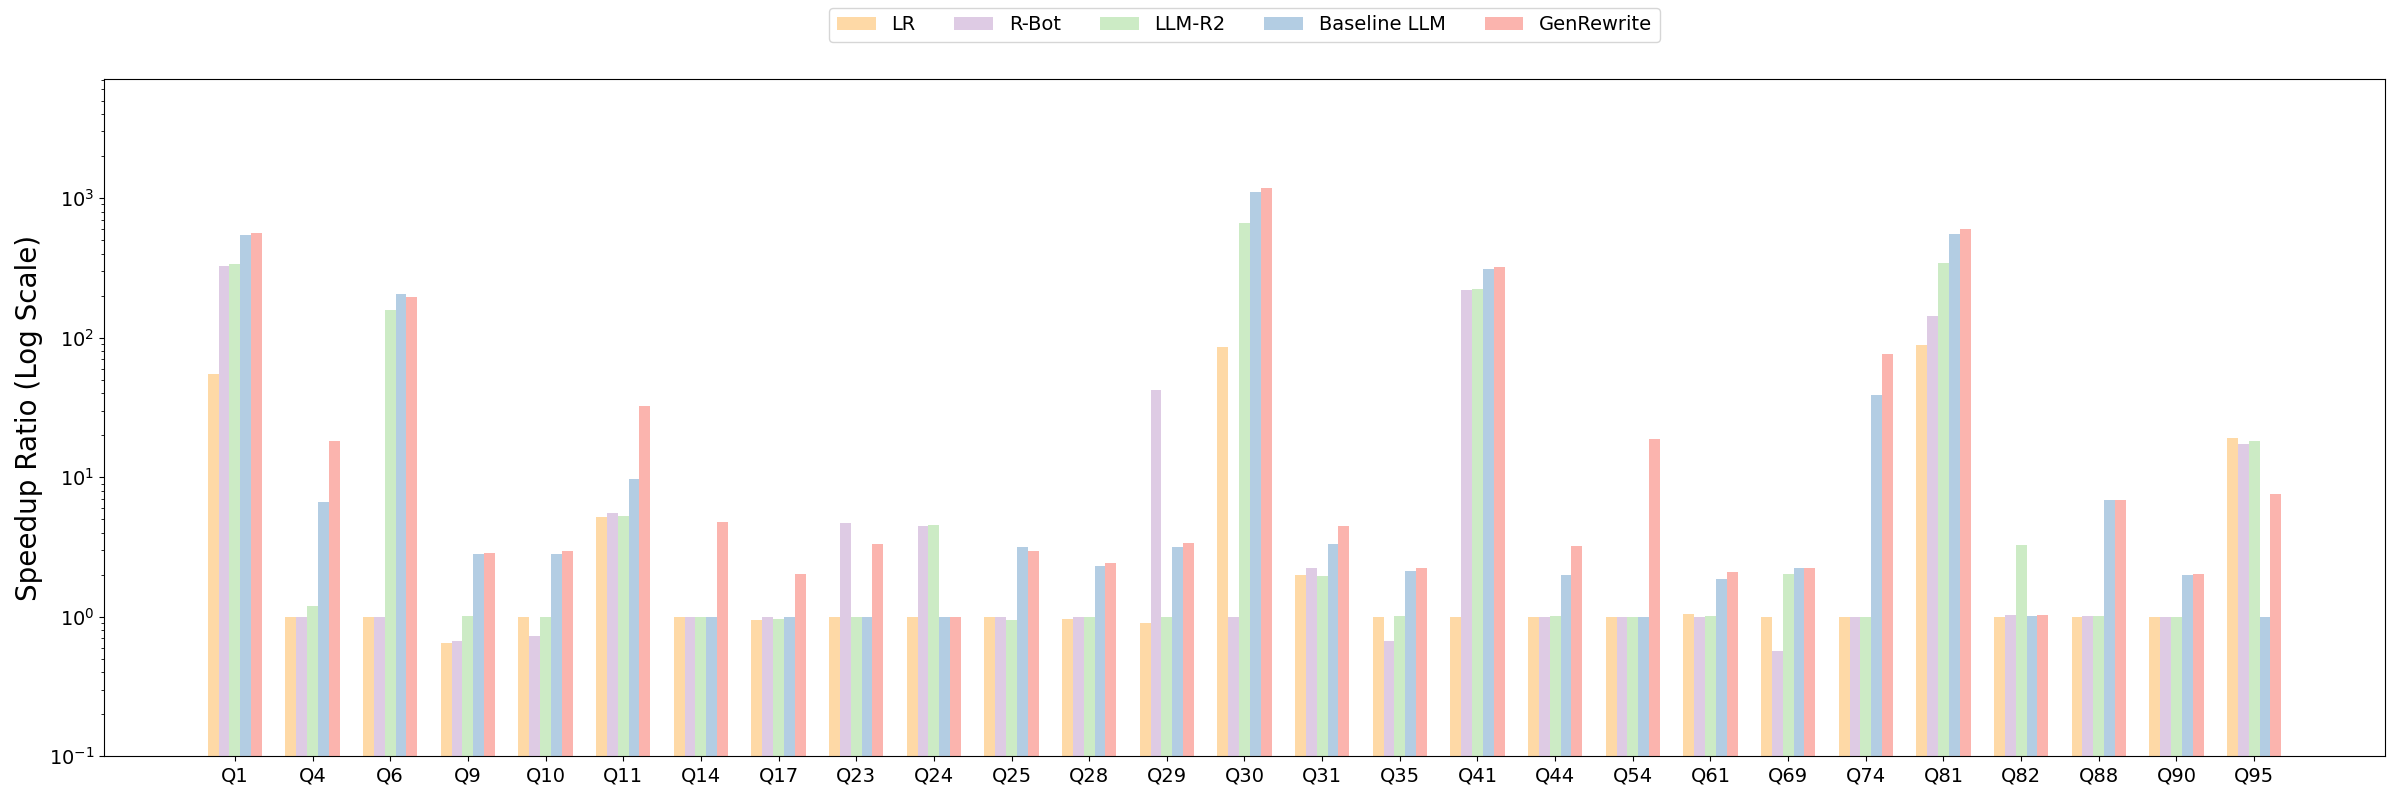
\includegraphics[width=\textwidth]{chapters/genrewrite/figures/baseline_comparison.png}
  \inv
  \vspace{-18pt}
  \captionsetup{font=small,name=Figure}
  \caption{Comparison of speedup achieved by different approaches on queries where at least one method attains a 2x or greater speedup. The y-axis is on a log scale.}
  \label{gen:fig:baseline}
  \inv
\end{figure*}

\end{comment}



\begin{comment}
    

In rule-based query rewriting, a set of pattern-matching rewrite rules define a fixed search space, resulting in consistent query outcomes across multiple runs. In contrast, due to the probabilistic nature of LLMs, 
    additional LLM runs increases the likelihood of uncovering new rewrite possibilities and thereby improving performance.
To ensure a fair comparison, we impose a limit on the number of LLM runs per query, 
    consistent with the setup outlined in Section~\ref{gen:sec:expr:llmbaseline}. Here, again, if a method fails to produce an equivalent rewrite for a particular query,  we deem the speedup ratio for that query as 1 indicating a fallback to the original query.
\end{comment}
% the number of iterations in \genrewrite to 5, including 4 i 
% a limit to the number LLM runs for each query in \genrewrite.

%  \genbarzan{check WA msg}
% \st{This predictability contrasts with the dynamic nature of LLM-based rewrites, where additional LLM runs increase the likelihood of uncovering new rewrite possibilities, potentially leading to significant performance boost.} 



% or if it is not applicable, \genbarzan{what does not applicable mean??}



\begin{comment}
    

\begin{table*}[h]
\centering
\begin{tabular}{lccccc}
\toprule
   & Syntax errors  & Semantic error & Regression (i.e., speedup < 1x) & >2x speedup \\
\midrule
\genrewrite & \textbf{4.3\%} &  \textbf{6.1\%}  & \textbf{2.0\%} & \textbf{21.2\%}  \\
Baseline LLM   & 30.3\%  & 29.3\% & 25.3\% & 10.1\% \\
\bottomrule
\end{tabular}
\caption{Comparison between \genrewrite and Baseline LLM on percentage of syntax error, syntax error, performance regression, more than 2x speedup}
\label{gen:tab:llmbaseline}
\end{table*}
\end{comment}


\subsection{Comparison with Rule-based Methods}
\label{gen:sec:expr:traditionalbaseline}


Analysis of Table.~\ref{gen:tab:speedup_all} shows that \genrewrite consistently surpasses the
three rule-based baselines in terms of the number of queries optimized, regardless of the desired speedup threshold, on all benchmarks. Other LLM-based methods also consistently outperform rule-based methods with smaller margins than \genrewrite.
We first consider the standard public benchmarks (Table~\ref{gen:tab:speedup_comparison}). On the original TPC-DS workload, \genrewrite identifies substantially more optimization opportunities than the rule-based baselines: it achieves at least 2x speedup on 25 queries, compared to 10, 9, and 6 queries for \textsc{LLM-R\textsuperscript{2}}, \rbot, and \lr, respectively. The advantage persists at higher thresholds (e.g., 10x speedup), and we observe a similar pattern on JOB. These results suggest that \genrewrite already outperforms established rule-based methods on well-studied public benchmarks.


\noindent\revtwo{SQLStorm workloads (Table~\ref{gen:tab:speedup_comparison_sqlstorm}) yield two key observations:}

\genhead{\revtwo{Observation 1}}
\revtwo{The performance gap between \genrewrite and the rule-based baselines widens on TPC-DS (SQLStorm).
    All three rule-based baselines (\textsc{LLM-R\textsuperscript{2}}, \rbot, and \lr) are built on top of Calcite and ultimately rely on Calcite’s rewrite rules. Their differences lie in rule selection and ordering, but they inherit the same two Calcite limitations: (1) \emph{Parser coverage:} The Calcite parser and validator do not fully support several constructs that appear in SQLStorm-generated  TPC-DS queries, such as recursive CTEs, \texttt{LENGTH}, etc. As a result, these systems only emit rewrites for roughly half of the input queries. (2) \emph{Rule coverage:} Even when Calcite can parse the query, its fixed rule set often fails to match the structure of these queries. SQLStorm's queries are not hand-polished benchmark SQL; they contain noisy nesting, ad hoc join predicates, and unseen operator combination that does not line up cleanly with Calcite’s stock transformations (e.g., predicate pushdown). In these cases, the systems may not show meaningful improvement. In contrast, \genrewrite does not depend on Calcite’s rule inventory. It can generate and iteratively refine rewrites for these same SQLStorm queries, which explains the widening gap on TPC-DS (SQLStorm).}

\genhead{\revtwo{Observation 2}}
\revtwo{On SQLStorm workloads, the ``LLM-enhanced'' rule-based systems degrade to the point that they can be outperformed by \lr, which does not use an LLM at all. \textsc{LLM-R\textsuperscript{2}} selects a few high-quality demonstration rewrites from a curated library using a learned retriever, and \rbot retrieves offline ``rewrite recipes'' mined from past queries. These strategies work on TPC-DS and JOB because the benchmark queries follow canonical patterns that are well represented in those demonstration pools. Under SQLStorm, however, the generated queries deviate substantially from those canonical patterns, so the retrieved demonstrations and recipes are often no longer relevant and provide poor guidance. \genrewrite, by contrast, is not limited to a static set of expert demonstrations or a fixed rule inventory. It employs iterative correction and accumulates transferable rewrite knowledge from prior queries, enabling it to adapt to new query forms without manual rule engineering.}



\revtwo{\genrewrite outperforms existing baselines both on the original TPC-DS / JOB benchmarks and on the SQLStorm-generated workloads. Its advantage becomes larger precisely in the regimes where fixed-rule systems provide poor coverage. If new rules were distilled from \genrewrite's successful rewrites on complex queries and then incorporated into Calcite, the rule-based methods could  be strengthened and extended to a broader class of queries.}



\genhead{\revtwo{A deeper look at rules discovered by \genrewrite}}
\revtwo{Besides standard Calcite rules (e.g., predicate pushdown, projection pruning), several papers propose more aggressive rewrite patterns for analytical workloads. Generalized Sub-Query Fusion~\cite{sarthi2020generalized} eliminates redundant I/O by fusing multiple similar subqueries into a single shared scan/aggregation. Super-operators~\cite{blitz2} collapse multi-branch aggregates and unions into a single streaming physical operator. The Spark engine in Azure Synapse~\cite{modi2021new} rewrites plans to reuse shuffles, push down filters and partial aggregates, and inject runtime partition pruning to reduce data movement. Athena~\cite{bruno2022computation} detects repeated expensive subplans in a query and fuses them so they are computed once and shared by all consumers. In Table~\ref{gen:tab:pattern-summary}, for each major rewrite pattern discovered by \genrewrite we ask: (1) does it align with any of these known patterns, at the idea level; and (2) is there an exact structural match already reported in prior work?}

% [leftmargin=0.5cm]

\noindent\revone{Representative optimization patterns discovered by \genrewrite:}
% \footnote{In Appendix~A, we present query pairs for each pattern and detail how they differ from prior work.}

\begin{enumerate}[leftmargin=0.5cm]
\item  \revone{Pivot with conditional aggregation instead of UNION-then-self-join.}
\item \revone{Replace multiple \texttt{EXISTS} conditions with a precomputed set via joins.}
\item \revone{Rewrite \texttt{COUNT(*)>0} as \texttt{EXISTS} (aggregate $\rightarrow$ semi-join; enables short-circuiting).}
\item \revone{Replace a bounded self-recursive CTE with a non-recursive base query \texttt{CROSS JOIN}ed to a small numbers table.}
\item \revone{Lift a per-key summary (e.g., item-level totals) into one CTE and drive all branches from it.}
\item \revone{Consolidate repetitive subqueries into a single aggregation subquery with conditional expressions.}
\item \revone{Decorrelate \texttt{IN} by joining a \texttt{SELECT DISTINCT} key,... mapping table instead of re-checking the subquery. }
\end{enumerate}


\begin{table}[tbp]
\inv
\small
\centering
\setlength{\tabcolsep}{6pt}
\def\arraystretch{1.2}

\begin{tabular}{ l | c c c }
\toprule
Pattern& Covered queries & Similar in idea & Exact match \\
\midrule
1 & 4, 11, 74 & ~\cite{blitz2}, ~\cite{bruno2022computation} & No \\
2 & 10, 35, 69 & ~\cite{begoli2018apache} & No \\
3 & 41 & ~\cite{begoli2018apache} & No \\
4 & 23998* &  & No \\
5 & 22722* & ~\cite{sarthi2020generalized}, ~\cite{bruno2022computation} & No \\
6 & 61, 88 & ~\cite{sarthi2020generalized}, ~\cite{bruno2022computation} & Yes,~\cite{bruno2022computation}  \\
7 & 28982*, 34389* & ~\cite{begoli2018apache} & Yes,~\cite{begoli2018apache}  \\
\bottomrule
\end{tabular}
\captionsetup{font=small,name=Table}
\caption{\revtwo{Summary of rewrite patterns discovered by \genrewrite. ``Covered queries'' lists the queries that exhibit each pattern (queries with * are from TPC-DS SQLStorm; others are from standard TPC-DS). ``Similar in idea'' notes prior work that proposes a conceptually related optimization. ``Exact match''indicates that the same structural rewrite has been reported before.}  }
\inv
\label{gen:tab:pattern-summary}
\end{table}











% \begin{enumerate}[leftmargin=0.5cm]

% \item  Pivot with conditional aggregation instead of UNION-then-self-join.
% \item Rewrite \texttt{COUNT(*)>0} as \texttt{EXISTS} (aggregate $\rightarrow$ semi-join; enables short-circuiting).
% \item Consolidate repetitive subqueries into a single aggregation subquery with conditional expressions.


% \end{enumerate}




\subsection{Detailed Analysis and Ablation Study}
\label{gen:sec:expr:ablation}

In this section, we conduct a detailed ablation study 
    to validate our design decisions in  \genrewrite and the contribution of each component therein towards the overall performance. We focus primarily on the \revtwo{original} TPC-DS benchmark, as its complexity provides a challenging test of our system's capabilities. The results, summarized in Table~\ref{gen:tab:ablation}, highlight the impact of individual components on LLM runtime overhead, monetary cost, and the percentage of queries achieving various levels of speedup.
    % To control for variables, we still adopt a setup in which our NLR2 repository is initialized with two LLM runs using the basic prompt and \genrewrite incorporates the NLR2 as a hint for the remaining two candidate rewrites,.


    




\begin{table*}[!t]
\small
\centering
\setlength{\tabcolsep}{5pt}
\def\arraystretch{1.1}
\vspace{-5pt}
\begin{tabular}{ | c | r r r r r |  }
\toprule
& \multicolumn{5}{c|}{TPC-DS} \\
 & >2x & >10x & >50x  & avg. time(s) & avg. cost(\$)  \\
\midrule
\genrewrite                           & \cntpct{25}{25.3} & \cntpct{9}{9.1}   & \cntpct{6}{6.1}   & 151.82 & 0.129 \\
\genrewrite without grouping NLR2s    & \cntpct{25}{25.3} & \cntpct{9}{9.1}   & \cntpct{6}{6.1}   & 385.47 & 0.310 \\
\genrewrite without bottleneck analysis & \cntpct{19}{19.2} & \cntpct{6}{6.1}   & \cntpct{5}{5.1}   & 150.30 & 0.124 \\
\genrewrite with gpt-4o               & \cntpct{14}{14.1} & \cntpct{5}{5.1}   & \cntpct{5}{5.1}   & 105.40 & 0.117 \\
\genrewrite with gpt-4-mini           & \cntpct{2}{2.0}   & \cntpct{1}{1.0}   & \cntpct{0}{0.0}   & 301.20 & 0.016 \\
\bottomrule
\end{tabular}
\captionsetup{font=small,name=Table}
\caption{Ablation study: impact of \genrewrite's design decisions on LLM runtime, cost, and the share of queries achieving various speedups.}
\label{gen:tab:ablation}
\vspace{-15pt}
\end{table*}



\genhead{Plan-based dominant NLR2 identification} This component plays a critical role in reducing query execution overhead, although its impact is not directly reflected in Table~\ref{gen:tab:ablation}. Without plan-based dominant NLR2 identification, we would need to execute each rewrite—generated by applying a single NLR2—to measure its runtime, which can be prohibitively expensive for long-running queries. 

\genhead{NLR2 grouping via LLM}
We collect an average of 5.08 NLR2s per input query after applying grouping, compared to 13.24 NLR2s per query without grouping. Although we only re-evaluate the impact of an NLR2 when the associated performance improvement exceeds a predefined threshold, grouping still significantly reduces both monetary and time costs. Without grouping, the average LLM runtime increases by 153.9\%, and the monetary cost rises by 140.3\%,  demonstrating that NLR2 grouping's impact on costs.


\genhead{Query performance bottleneck analysis} 
We compare two strategies: (1) apply the top NLR2s globally, ignoring query similarity; and (2) our default, which retrieves candidates by bottleneck similarity. The global strategy performs essentially the same as \baseline, indicating that ``best overall'' strategy rarely transfers. Bottleneck-aware retrieval, in contrast, delivers clear gains: effective reuse hinges on aligning NLR2s with performance bottlenecks.

% We evaluate two strategies for identifying queries with similar performance bottlenecks: (1) applying the top beneficial NLR2s regardless of query similarity, and (2) our default approach, which incorporates bottleneck-aware retrieval. Experimental results show that the first strategy performs nearly identically to \baseline, suggesting that indiscriminately applying high-performing NLR2s provides little benefit. This underscores the importance of relevance—effective reuse of NLR2s depends on accurately identifying queries with comparable performance bottlenecks.



\genhead{Choice of the LLM}
\genrewrite's performance critically depends on the LLM's reasoning capabilities. We evaluate three models: OpenAI’s \texttt{o3-mini} (reasoning-oriented), \texttt{gpt-4o} (balanced), and \texttt{gpt-4o-mini}(most cost-efficient).  \genrewrite powered by \texttt{gpt-4o} is noticeably outperformed by the \texttt{o3-mini} variant. We decompose \genrewrite’s workflow into two stages: (1) discovering effective rewrites and summarizing NLR2s, and (2) applying high-quality NLR2s to guide rewrites. We observe that \texttt{gpt-4o} struggles primarily in stage 1. However, when \genrewrite with \texttt{gpt-4o} is supplied with NLR2s previously discovered by \texttt{o3-mini}, the number of queries achieving a speedup $\geq$ 10× increases from 5 to 8,  further demonstrating the effectiveness of NLR2-guided rewriting.
% \texttt{gpt-4o-mini} rarely produces useful rewrites.



% \genrewrite’s gains track the model’s reasoning strength. \texttt{o3-mini} (reasoning-oriented) consistently finds stronger rewrites and better NLR2s, outperforming \texttt{gpt-4o}; \texttt{gpt-4o-mini} rarely produces useful rewrites. Decomposing \genrewrite into (i) discovery/summarization of NLR2s and (ii) application shows where the gap arises: \texttt{gpt-4o} underperforms in (i) but applies good NLR2s well—when seeded with \texttt{o3-mini}’s NLR2s, its count of >10× speedups rises from 5 to 8. Practical takeaway: use the strongest model for discovery, then a cheaper model can reliably apply the learned NLR2s.


\genhead{\revone{Parameter sensitivity analysis}}




\begin{table}[tbp]
\small
\centering
\begin{tabular}{l*{4}{cc}}
\toprule
& \multicolumn{2}{c}{$k{=}1$}
& \multicolumn{2}{c}{$k{=}2$}
& \multicolumn{2}{c}{$k{=}3$}
& \multicolumn{2}{c}{$k{=}4$} \\
\cmidrule(lr){2-3}
\cmidrule(lr){4-5}
\cmidrule(lr){6-7}
\cmidrule(lr){8-9}
& eq & fast
& eq & fast
& eq & fast
& eq & fast \\
\midrule
No correction
& 52 & 5
& 67 & 8
& 70 & 12
& 74 & 21 \\
Semantic only
& 54 & 5
& 68 & 10
& 71 & 14
& 75 & 21 \\
\textbf{Semantic + syntax}
& \textbf{70} & \textbf{5}
& \textbf{79} & \textbf{10}
& \textbf{85} & \textbf{16}
& \textbf{86} & \textbf{28} \\
\bottomrule
\end{tabular}
\captionsetup{font=small,name=Table}
\caption{\revone{Cumulative count of queries with (i) at least one equivalent rewrite (\textit{equiv}) and (ii) at least one equivalent rewrite that is at least 20\% faster than the original (\textit{faster}), as the candidate budget increases ($k{=}1\ldots4$), under different correction strategies.}}
\label{gen:tab:correction_ablation_new}
\inv
\end{table}


\noindent\revone{
\emph{\textbf{Budget:}} maximum candidates per query \(K=4\); correction caps \(I_{\mathrm{sem}}=I_{\mathrm{syn}}=3\) (semantic and syntax loops). For the TPC-DS workload, the average iterations is 0.30 (semantic) and 0.76 (syntax). The per-query correction iteration distributions are:}
\begin{itemize}
    \item \revone{Semantic: 0: 76.72\%, 1: 19.02\%, 2: 1.64\%, 3: 2.62\%.}
    \item \revone{Syntax: 0: 60.66\%, 1: 18.36\%, 2: 5.25\%, 3: 15.74\%.}
\end{itemize}
\revone{We vary the candidate budget $k \in\{1,2,3,4\}$. Table~\ref{gen:tab:correction_ablation_new} reports the \emph{cumulative} number of queries that achieve (i) $\geq 1$ equivalent rewrite and (ii) $\geq 1$ equivalent rewrite that is at least 20\% faster, as $k$ increases (higher \(k\) means more candidates attempted per input query), comparing: (i) no correction, (ii) semantic-only correction, and (iii) semantic\,+\,syntax correction.} \revone{Table~\ref{gen:tab:correction_ablation_new} shows that correction loops markedly reduce the effective error rate,  with \emph{semantic + syntax} outperforming the other settings at every \(k\). Larger \(k\) improves coverage with diminishing returns and proportionally higher cost.}


\noindent\revone{\emph{\textbf{Desired speedup threshold:}}
We set $\theta$ to 1.2x in our implementation. Increasing $\theta$ reduces coverage  but raises the average speedup among accepted rewrites. With a lower $\theta$, we keep more rewrites — including many that are only modestly better.}

\begin{table}[H]
\small
\centering
\begin{tabular}{lccc}
\toprule
Desired speedup threshold $\theta$ & 1.2x & 2.0x & 5.0x \\
\midrule
Coverage (\%)       & 28.3 & 23.2 & 13.1 \\
Geom.\ mean speedup & 11.1x & 17.0x & 72.2x \\
\bottomrule
\end{tabular}
\captionsetup{font=small,name=Table}
\caption{\revone{Coverage and geometric mean speedup for desirable speedup thresholds $\theta \in \{1.2x,1.5x,2.0x\}$. 
Coverage(\%) is the fraction of queries with $\ge\theta$ speedup; geom.\ mean is over covered queries.}}
\label{gen:tab:theta_sweep}
\inv
\end{table}

\vspace{-5mm}

\genhead{\revthree{Counterexample-guided iterative correction}} 
\revthree{We compare our counterexample-based semantic check to Miniature \& Mull from LLM-SQL-Solver~\cite{zhao2023llm} on random TPC-DS rewrites (no correction). Our prompt yields 29\% equivalent rewrites before syntax correction with a 6\% false-positive rate; Miniature \& Mull achieves 26\% equivalents with 22\% false positives. Thus our prompt better aligns with the iterative correction task—more verified equivalents and far fewer false positives.}



% \revthree{LLM-SQL-Solver~\cite{zhao2023llm} introduces the Miniature \& Mull prompting strategy for equivalence checking, which also searches for counterexamples and bases the decision on them. For a head-to-head comparison, we replaced our semantic-checking prompt with theirs and evaluated both settings on randomly sampled TPC-DS rewrites without any correction. With our prompt—which asks the LLM to produce a concrete counterexample and then feeds it back as a hint for semantic correction—we obtain 29\% equivalent rewrites \emph{before} syntax correction stage and a 6\% false-positive rate (inequivalent rewrites judged equivalent). Using Miniature \& Mull, we observe 26\% equivalent rewrites and a 22\% false-positive rate under the same protocol. This indicates our semantic-checking prompt is better aligned with the rewrite-correction loop, yielding more verified equivalents while substantially reducing false positives.}


% LLM-SQL-Solver proposes Miniature and Mull prompting technique for equivalence checking, which shares similar idea with our method about finding counterexamples and then give the conclusion. We replace our semantic checking prompt with theirs and test both on TPC-DS workloads. The result shows that with our semantic checking prompt which asks for a counterexample from LLMs and then be used as the hints for semantic corrections, we get 29\% equivalent queries (before syntax correction) and 6\%  false positive (LLMs consider the inequivalent rewrites to be equivalent). For LLM-SQL-Solver, we get 26\% equivalent queries and 22\% false positives. Our semantic checking prompt suits better with this rewrite correction task.














\begin{comment}


\genhead{Impact of semantic   and syntax correction} For each TPC-DS query, we conduct 4 independent runs to generate 4 candidate rewrites. In each run, we use zero-shot prompting (Baseline LLM) to suggest candidate queries and adopt one of the following correction strategies before assessing the correctness and performance of the rewrite.

\begin{enumerate}
    \item No correction.
    \item Only semantic correction.
    \item Only syntactic correction.
    \item Two-stage correction (semantic correction and then syntax correction).
\end{enumerate}



\noindent We set the maximum iteration count 3 for both semantic and syntax correction.

Table~\ref{gen:tab:correction_ablation} compares cumulative equivalent rewrites generated by various correction strategies over successive runs, with each cell showing the number of TPC-DS queries equivalently rewritten by a specific strategy up to that point (the highest possible is 99). The analysis clearly demonstrates that the two-stage correction strategy outperforms others, and not applying any correction yields the least effective results, with the remaining strategies falling in between. In a direct comparison between ``Only semantic correction'' and ``Only syntax correction'', the latter shows a quicker ability to produce executable and equivalent rewrites for simpler queries in the first few runs. However, its effectiveness is limited by a lower ceiling due to a lack of understanding regarding the queries' intent, leading to executable but inequivalent rewrites for more complex queries. When combining these two strategies together, semantic correction interprets the intent, ensuring the rewrite's objectives align with the original query, and then syntax correction refines the rewrite to be executable. The two-stage strategy (i.e., semantic + syntax) identifies equivalent rewrites for 70 of the 99 TPC-DS queries in the first run. It then adds 3 more in the second run and 6 in the third, ultimately achieving equivalent rewrites for 90 of the 99 queries.



\begin{table}[h]
\centering
\begin{tabular}{lcccc}
\toprule
 & run 1 & run 2 & run 3 & run 4 \\
\midrule
No correction & 45 & 56 & 65 & 69  \\
Only semantic & 51 & 66 & 76 & 82 \\
Only syntactic & 60 & 68 & 73 & 76 \\
\textbf{Semantic + syntactic} & \textbf{70} & \textbf{81} & \textbf{87} & \textbf{90} \\
\bottomrule
\end{tabular}
\caption{Cumulative count of equivalent rewrites   using different correction strategies over multiple runs.}
\label{gen:tab:correction_ablation}
\inv
\end{table}



Delving deeper into the two-stage correction strategy, it generally achieves convergence quickly, usually within 3 iterations, except for a small number of cases involving overly complex queries. However, there is still a gap between the queries deemed equivalent by the LLM and those that are truly equivalent. The non-cumulative count of queries  verified as equivalent in each run are 69, 75, 69, and 70, respectively.  When aggregating results from all runs, 90 unique queries are   equivalent, indicating that the sets of queries identified as equivalent in each run vary.




    

\genhead{Impact of NLR2s as hints}  After conducting 4 rounds of zero-shot prompting, we reach a stable state where additional rounds fail to bring improvements in terms of the number of rewrites that are both equivalent and faster.
This suggests that we effectively capture most of low-hanging fruits. A comparative analysis between an additional iteration using zero-shot prompting and another leveraging prompts augmented with specific NLR2 hints reveals a pronounced superiority of the latter. The queries solvable exclusively through hint-augmented prompts 
are presented in Table~\ref{gen:tab:knowledge_ablation}.


% Two crucial observations are highlighted in Section 3: LLMs are more likely to struggle in identifying rewrite opportunities with increasing query complexity; LLMs can optimize queries that they previously struggled to optimize when provided with suitable hints in the prompt. The primary goal of employing NLR2s is to facilitate knowledge transfer and bridge the gap between queries that LLMs can optimize without hints and those they cannot, enabling LLMs to optimize a broader range of queries.

% \begin{table}[ht]
% \centering
% \caption{Rewrite hints .}
% \label{gen:tab:knowledge_ablation}
% \begin{tabular}{lccccc}
% \toprule
%  & Q4 & Q11 & Q20 & Q29 & Q76 \\
% \midrule
% Without hints & - & 1.07x & 1x & 1.42x & 1x  \\
% With hints & \textbf{5.68x} & \textbf{10.3x} & \textbf{9.89x} & \textbf{6.85x} & \textbf{9.77x} \\
% \bottomrule
% \end{tabular}
% \end{table}


% \begin{table}[h]
% \centering
% \caption{NLR2s inspired speedups}
% \label{gen:tab:knowledge_ablation}
% \begin{tabular}{ccc p{4cm}}
% \toprule
% input & speedup & inspired by & \small{NLR2s} \\
% \hline
% 4 & 5.68x & 74 &  \footnotesize{Avoid UNION ALL if not necessary \newline Split complex queries into simpler ones using WITH clause} \\ \hline
% 11 & 10.3x & 74 & \footnotesize{Avoid UNION ALL if not necessary \newline Split complex queries into simpler ones using WITH clause} \\ \hline
% 20 & 9.89x & 12 &  \footnotesize{Use CTE (Common Table Expressions) to break down complex queries \newline Reduce the number of tables in the join operation} \\ \hline
% 29 & 6.85x & 25 &  \footnotesize{Aggregate before join \newline Use subqueries to break down complex queries} \\ \hline
% 76 & 9.77x & 61 &  \footnotesize{Combine multiple queries into a single query \newline Move WHERE clause filters to ON clause in JOINs} \\
% \bottomrule
% \end{tabular}
% \end{table}





Q4, Q11, and Q74 all see improvements by eliminating the unnecessary \sqlunionallcolor, which has been discussed in earlier sections. Q20 benefits from NLR2s learned from its neighboring query Q12. Inspired by the rule ``Use CTE to break down complex queries'', the actual transformation applied is a group-by pushdown. Q29 is solved using similar ideas but exhibits a different query pattern and learns from Q25.
For Q76,  where multiple segments each join two common tables across several subqueries, the rewrite strategy is to combine these segments with \sqlunionallcolor before conducting a join with the common tables, thereby avoiding duplicate computation. This strategy is inspired by the rule ``Combine multiple queries into one query'' from Q61. These instances underscore the value of employing NLR2s for effective knowledge transfer across queries. At the conclusion of our experiments, we collect 156 groups of rewrite rules,  with an average of 7 rules per group.
\end{comment}

\begin{comment}
    

\genhead{\texttt{EXPLAIN} cost vs. actual latency} When evaluating rewrites, we can either utilize the database's own cost estimates as a surrogate for actual performance (i.e., using \texttt{EXPLAIN}) 
or measure the latency by actually running candidate queries directly on the database or a small sample of it. The latter approach, while offering greater accuracy, also results in higher costs, which is justifiable when the query is optimized once and rewritten many times (see target use case in \S\ref{gen:sec:intro}). The goal of this experiment is to quantify the negative impact of using 
inaccurate cost estimates on \genrewrite's performance.

We examine two variants of \genrewrite, differing only in their choice of evaluation metric. One variant calculates the utility scores of NLR2s   based on actual latency while the other relies on \texttt{EXPLAIN}'s cost estimates. 
The comparison between the two variants is detailed in 
Table~\ref{gen:tab:latency_vs_cost}. We observe that both coverage and latency reduction ratios are lower when \texttt{EXPLAIN} is used for query evaluation. This is expected: (1) cost estimates do not accurately reflect actual latency, meaning a rewrite with a lower cost estimate does not guarantee lower latency; (2) the speedup ratios derived from cost estimates can be disproportionately high, not aligning with the actual latency improvements, thereby impacting the effectiveness of NLR2s. Despite these issues, the variant that rely on \texttt{EXPLAIN} cost still outperforms all other baselines.

\end{comment}








\subsection{Time and Monetary Cost}
% \subsection{Cost analysis of LLM}
\label{gen:sec:expr:llmcost}


While \genrewrite’s time and API costs are a one-time, amortized expense for recurring workloads (see Target workloads in \S\ref{gen:sec:intro}), we still quantify them to ensure they remain modest. Using OpenAI’s \texttt{o3-mini} to generate a rewrite for a TPC-DS query—including suggestion, semantic correction, and syntactic correction—costs on average \$0.029 and takes 36.15 s. For comparison, \texttt{gpt-4o} and \texttt{gpt-4o-mini} average (\$0.026, 25.1 s) and (\$0.004, 71.71 s), respectively. As a reasoning-focused model, \texttt{o3-mini} consumes more tokens, increasing cost but often yielding more logically sound, well-structured rewrites for complex SQL transformations. Auxiliary LLM steps (e.g., grouping NLR2s and selecting the bottleneck) add negligible overhead. Overall, total cost scales approximately linearly with the number of candidate rewrites generated by the pipeline.


%  Although the time and monetary cost of \genrewrite is not as relevant given that it is a one-time cost that gets amortized for recurrent workloads (see Target workloads in \S\ref{gen:sec:intro}), we still need to ensure they do not become excessive.
% Using OpenAI’s \texttt{o3-mini} model to generate a rewrite for a TPC-DS query—including rewrite suggestion, semantic correction, and syntactic correction—incurs an average cost of approximately \$0.029 and takes 36.15 seconds. For comparison, \texttt{gpt-4o} and \texttt{gpt-4o-mini} yield average costs and durations of (\$0.026, 25.1 seconds) and (\$0.004, 71.71 seconds), respectively. \texttt{o3-mini}, being a reasoning-focused model, tends to consume significantly more tokens during generation. While this leads to higher total costs, the increased token usage contributes to more logically sound and well-structured rewrites, especially in the context of complex SQL transformation tasks.
% The cost associated with auxiliary LLM tasks, such as grouping NLR2s and selecting the most relevant bottleneck  is negligible in practice. Overall, the total cost of the system grows linearly with the number of candidates generated with the rewriting pipeline.


% Although \texttt{gpt-4o} is approximately twice as expensive per token as \texttt{o3-mini}, and roughly 16 times more expensive than \texttt{gpt-4o-mini}, our experiments show that the overall cost of using \texttt{o3-mini} is actually higher than that of \texttt{gpt-4o}. This counterintuitive result stems from the fact that \texttt{o3-mini}, being a reasoning-focused model, tends to consume significantly more tokens during generation. While this leads to higher total costs, the increased token usage contributes to more logically sound and well-structured rewrites, especially in the context of complex SQL transformation tasks.
% The cost associated with auxiliary LLM tasks, such as grouping NLR2s and selecting the most relevant bottleneck from the top-$k$ candidates—is negligible in practice. Overall, the total cost of the system grows linearly with the number of iterations of the rewriting pipeline.



\begin{table}[h]
% \small
\footnotesize
\centering
\setlength{\tabcolsep}{6pt}
\def\arraystretch{1.1}
\vspace{-5pt}
\begin{tabular}{  c | r r r | r r r }
\toprule
& \multicolumn{3}{c|}{time (s)} 
& \multicolumn{3}{c}{monetary cost (\$)} \\
stage & suggest & \makecell{semantic\\corr.} & \makecell{syntax\\corr.} & suggest & \makecell{semantic\\corr.} & \makecell{syntax\\corr.} \\
\midrule
o3-mini     & \makecell{5.8\\(16.0\%)} & \makecell{20.8\\(57.6\%)}  & \makecell{9.6\\(26.5\%)}  & \makecell{7.8e-03\\(26.4\%)} & \makecell{1.5e-02\\(52.2\%)}  & \makecell{6.3e-03\\(21.3\%)} \\
gpt-4o & \makecell{1.5\\(5.8\%)} & \makecell{22.1\\(87.9\%)}  & \makecell{1.6\\(6.3\%)}  & \makecell{6.4e-03\\(23.9\%)} & \makecell{1.9e-02\\(70.1\%)}  & \makecell{1.6e-03\\(6.0\%)} \\
gpt-4o-mini & \makecell{1.9\\(2.6\%)} & \makecell{66.8\\(93.1\%)}  & \makecell{3.1\\(4.3\%)}  & \makecell{4.0e-04\\(11.2\%)}  & \makecell{3.1e-03\\(84.6\%)}   & \makecell{1.5e-04\\(4.2\%)} \\
% \rbot       & \makecell{9\\(9.1\%)}  & \makecell{5\\(5.1\%)}   & \makecell{3\\(3.0\%)}   & \makecell{7\\(6.2\%)}  & \makecell{3\\(2.7\%)}   & \makecell{2\\(1.8\%)} \\
% \lr       & \makecell{6\\(6.1\%)}  & \makecell{4\\(4.0\%)}   & \makecell{0\\(0\%)}   & \makecell{6\\(5.3\%)}  & \makecell{2\\(1.8\%)}   & \makecell{1\\(0.9\%)} \\
\bottomrule
\end{tabular}
\captionsetup{font=small,name=Table}
\caption{\small LLM cost analysis: the monetary and time cost of generating one rewrite candidate for a TPC-DS query, including all three stages--- rewrite suggestions, semantic correction, and syntactic correction.}
\inv
\label{gen:tab:llm_cost}
\vspace{-10pt}
\end{table}

 
 % The breakdown of the monetary and time cost is presented in Table~\ref{gen:tab:llm_cost}. Across all three models, semantic correction phase accounts for the highest cost in terms of both monetary and time cost. However, when using \texttt{o3-mini}, a larger portion of time is also spent on the candidate suggestion and syntax correction phases. This is because \texttt{o3-mini}, with its stronger reasoning capabilities, tends to better understand the input query and generate more aggressive rewrites. While this increases the likelihood of discovering high-quality transformations, it also lowers the chance of producing equivalent rewrites on the first attempt, thereby requiring additional iterations in the syntax correction phase. In contrast, the two lower-capacity models exhibit a more conservative rewriting style, leading to fewer iterations but also fewer opportunities for substantial performance improvement.

 Table~\ref{gen:tab:llm_cost} shows that semantic correction dominates both time and cost across models. With \texttt{o3-mini}, more time also goes to candidate suggestion and syntax correction: its stronger reasoning yields more aggressive rewrites (more chances for big wins) but requires extra iterations to ensure equivalence. By contrast, \texttt{gpt-4o} and \texttt{gpt-4o-mini} rewrite more conservatively, needing fewer iterations but offering fewer opportunities for substantial speedups.

\revone{For equivalence checking, we set a 60 sec timeout for the tester and 5 sec for the verifier. Performance–evaluation time varied by query from seconds to hours. We also terminated execution early when a candidate failed to exceed the original query by the desired speedup threshold $\theta$.}

 


% \subsection{Choice of the LLM}
% \label{gen:sec:expr:llmchoice}

% The performance of components in \genrewrite critically depends on the knowledge and reasoning capabilities of the chosen LLM. If an LLM fails to optimize queries, no transferable knowledge is generated, and if it does not accurately capture a query’s objective, it is unlikely to identify relevant counterexamples. We evaluate three LLMs with varying costs and capabilities: OPENAI o3-mini, which excels at reasoning; gpt-4, the state-of-the-art general-purpose model; and gpt-3.5-turbo, which provides basic text understanding. As shown in Table~\ref{gen:tab:ablation}, OPENAI o3-mini achieves the best speedup statistics at a modest cost, demonstrating both the rapid progress in language models for complex tasks and the powerful reasoning capabilities even in small-scale models.





% \genhead{LLM's capacity}






% evaluating queries with explain costs or actual latency


% \noindent\textbf{Compared approaches.} To understand the contribution of various components within our tool, we remove certain components to compare its performance with that of the complete tool.

% \begin{itemize}
%     \item \textbf{Zero-shot prompts with no correction.}
%     \item \textbf{Zero-shot prompts with only semantic correction.}
%     \item \textbf{Zero-shot prompts with only syntax correction.}
%     \item \textbf{Zero-shot prompts with two-stage correction.}
%     \item \textbf{Prompts with rewrite hints (\texttt{EXPLAIN} cost).}
%     \item \textbf{Prompts with rewrite hints (actual latency).}
%     \item \textbf{}
%     \item 
    
% \end{itemize}



\begin{comment}
    
\begin{table}[!t]
\small
\centering
\setlength{\tabcolsep}{6pt}
\def\arraystretch{1.1}

\vspace{-5pt}
\begin{tabular}{  c | r r r | r r r }
\toprule
& \multicolumn{3}{c|}{TPC-DS} 
& \multicolumn{3}{c}{JOB} 
%& \multicolumn{2}{c|}{TPC-H} 
%& \multicolumn{2}{c}{TPC-DS} 
\\ 
speedup & >2x 
& >10x
& >50x 
& >1.2x 
& >2x
& >10x 
%& median 
%& max 
%& median 
%& max 
\\ 
\midrule
\genrewrite
& {25} & {9} & 
 {6}	&  {24}	& 8
& 3 
 %& \ruirevisiontbd{4.15}  &  \ruirevisiontbd{4.58}	 &  \ruirevisiontbd{5.03}		& \ruirevisiontbd{5.74}
\\ 
\baseline
& 18 & 6 & 5	& 19	 & 7
& 3 
%& 0.25 & 	1.58 & 	2.48	& 25.51 
\\ 
\textbf{LLM-R\textsuperscript{2}}
& 10	& 6 &	5	& 9	& 2
& 1 
%& 0.36	& 0.36	& NA &	NA 
\\ 
\lr
& 6	& 4 &	0	& 6	& 2
& 1
%& 0.36	& 0.36	& NA &	NA 
\\ 

\bottomrule
\end{tabular}
\caption{\small Speedup.}
\label{gen:tab:f}
\vspace{-15pt}
\end{table}
\end{comment}



\begin{comment}
    Since LLMs operate probabilistically, more trials increase the chances of finding a better rewrite. However, this is impractical due to time and cost constraints. Therefore, a system that more effectively uncovers hidden rewrite opportunities can significantly reduce both computational expenses and execution time.

From Table~\ref{gen:speedup_comparison}, we could see that both LLM-based 
which could be easily explained as LLMs have accumulated a solid knowledge base from the massive training data

\end{comment}


\begin{comment}
     Table~\ref{gen:tab:llmbaseline} shows a direct comparison between \genrewrite and  Baseline LLM. 
Notably, 30.3\% of  Baseline LLM's rewrites  are unexecutable (due to syntax error), compared to only 4.3\% for \genrewrite. The percentage of rewrites leading to semantic errors (i.e., non-equivalent rewrites) for Baseline LLM is 29.3\%, compared to only 6.1\% for \genrewrite. Both results demonstrate the effectiveness of our iterative correction strategy.


%marginally higher than BaselineLLM's 18.7\%, a result that initially appears surprising. In fact, it does not imply that \genrewrite's syntax correction is useful while its semantic correction is flawed. An unexecutable rewrite may indicate either a syntax error or both syntax and semantic errors, meaning SemanE does not accurately capture the ratio of semantic errors. A significant portion of SynE also has semantic errors.

\genrewrite results in only 2 performance regressions from 93 queries with equivalent rewrites-—-defined as those with over 5\% longer execution time than the original query--—while Baseline LLM experiences 23 performance regressions out of 70 equivalent rewrites. Moreover, \genrewrite achieves more than a 2x speedup in its rewrites twice as often as Baseline LLM. There two statistics show the effectiveness of our knowledge transfer.

% \genrewrite has a 25\% chance of generating incorrect queries, significantly lower than Baseline LLM's 49\%. Consequently, \genrewrite can produce equivalent rewrites for 93.9\% of TPC-DS queries, compared to Baseline LLM's 70.7\%. When selecting the best rewrites for comparison with the input queries, 

Overall, these results show the effectiveness of \genrewrite in drastically improving the quantity and quality of rewrites that one can achieve by na\"ively invoking the LLM.


Separate evaluation of NLR2s not only identify the exact contribution of each NLR2 but also find the NLR2 that leads to inequivalence. For example

\end{comment}


\begin{comment}
    
\begin{table}[tb]
\centering
\begin{tabular}{lccccc}
\toprule
speedup & >10\% & >50\% & >2x & >10x & >100x \\
\midrule
Using latency & \textbf{33.3\%} & \textbf{24.2\%} & \textbf{21.2\%} & \textbf{9.1\%} & \textbf{3.0\%} \\
Using \texttt{EXPLAIN} cost & 23.2\% & 16.2\% & 13.1\% & 7.1\% & \textbf{3.0\%} \\
\bottomrule
\end{tabular}
\caption{Comparison of the percentage of queries optimized when using latency and \texttt{EXPLAIN} cost as the evaluation metric}
\label{gen:tab:latency_vs_cost}
\inv
\end{table}
\end{comment}



\begin{comment}
    \begin{table}[tb]
\inv
\centering
\setlength{\tabcolsep}{3pt} % Adjust the space between columns
\begin{tabular}{@{}cccp{4.5cm}@{}}
\toprule
input & speedup & inspired by & \small{NLR2s} \\
\midrule
Q4 & 5.68x & Q74 &  \footnotesize{Avoid UNION ALL if not necessary; \newline Split complex queries into simpler ones using WITH clause} \\
Q11 & 10.3x & Q74 & \footnotesize{Avoid UNION ALL if not necessary; \newline Split complex queries into simpler ones using WITH clause} \\
Q20 & 9.89x & Q12 &  \footnotesize{Use CTE (Common Table Expressions) to break down complex queries; \newline Reduce the number of tables in the join operation} \\
Q29 & 6.85x & Q25 &  \footnotesize{Aggregate before join; \newline Use subqueries to break down complex queries} \\
Q76 & 9.77x & Q61 &  \footnotesize{Combine multiple queries into a single query; \newline Move WHERE clause filters to ON clause in JOINs} \\
\bottomrule
\end{tabular}
\caption{NLR2s inspired speedups}
\label{gen:tab:knowledge_ablation}
\inv
\end{table}
\end{comment}


\begin{comment}
    \begin{table}[H]
\small
\centering
\begin{tabular}{lcccc}
\toprule
 & \(k{=}1\) & \(k{=}2\) & \(k{=}3\) & \(k{=}4\) \\
\midrule
No correction & 52 & 67 & 70 & 74 \\
Semantic only & 54 & 68 & 71 & 75 \\
\textbf{Semantic + syntax} & \textbf{70} & \textbf{79} & \textbf{85} & \textbf{86} \\
\bottomrule
\end{tabular}
\captionsetup{font=small,name=Table}
\caption{Cumulative count of queries with $\geq$1 equivalent rewrites as the candidate budget increases (\(k=1\ldots 4\)), under different correction strategies.}
\label{gen:tab:correction_ablation}
\inv
\end{table}
\end{comment}




\begin{comment}


\begin{table}[H]
\small
\centering
\setlength{\tabcolsep}{6pt}
\def\arraystretch{1.1}
\vspace{-5pt}
\begin{tabular}{  c | r r r | r r r }
\toprule
& \multicolumn{3}{c|}{TPC-DS} 
& \multicolumn{3}{c}{JOB} \\
speedup & >2x & >10x & >50x & >1.2x & >2x & >10x \\
\midrule
\genrewrite     & \makecell{25\\(25.3\%)} & \makecell{9\\(9.1\%)}  & \makecell{6\\(6.1\%)}  & \makecell{20\\(17.7\%)} & \makecell{8\\(7.1\%)}  & \makecell{3\\(2.7\%)} \\
\baseline & \makecell{18\\(18.2\%)} & \makecell{6\\(6.1\%)}  & \makecell{5\\(5.1\%)}  & \makecell{19\\(16.9\%)} & \makecell{7\\(6.2\%)}  & \makecell{3\\(2.7\%)} \\
\lithe & \makecell{16\\(x\%)} & \makecell{6\\(6.1\%)}  & \makecell{4\\(x\%)}  & \makecell{17\\(x\%)} & \makecell{6\\(x\%)}  & \makecell{1\\(x\%)} \\
\textsc{LLM-R\textsuperscript{2}} & \makecell{10\\(10.1\%)} & \makecell{6\\(6.1\%)}  & \makecell{5\\(5.1\%)}  & \makecell{9\\(8.0\%)}  & \makecell{2\\(1.8\%)}   & \makecell{1\\(0.9\%)} \\
\rbot       & \makecell{9\\(9.1\%)}  & \makecell{5\\(5.1\%)}   & \makecell{3\\(3.0\%)}   & \makecell{7\\(6.2\%)}  & \makecell{3\\(2.7\%)}   & \makecell{2\\(1.8\%)} \\
\lr       & \makecell{6\\(6.1\%)}  & \makecell{4\\(4.0\%)}   & \makecell{0\\(0\%)}   & \makecell{6\\(5.3\%)}  & \makecell{2\\(1.8\%)}   & \makecell{1\\(0.9\%)} \\
\bottomrule
\end{tabular}
\captionsetup{font=small,name=Table}
\caption{Speedup Comparison between all methods on original TPCDS and JOB workloads.}
\label{gen:tab:speedup_comparison}
\vspace{-15pt}
\end{table}



\begin{table}[H]
\small
\centering
\setlength{\tabcolsep}{6pt}
\def\arraystretch{1.1}
\vspace{-5pt}
\begin{tabular}{  c | r r r | r r r }
\toprule
& \multicolumn{3}{c|}{TPC-DS (SQLStorm)} 
& \multicolumn{3}{c}{JOB (SQLStorm)} \\
speedup & >2x & >10x & >50x & >1.2x & >2x & >10x \\
\midrule
\genrewrite     & \makecell{25\\(25.3\%)} & \makecell{9\\(9.1\%)}  & \makecell{6\\(6.1\%)}  & \makecell{20\\(17.7\%)} & \makecell{8\\(7.1\%)}  & \makecell{3\\(2.7\%)} \\
\baseline & \makecell{18\\(18.2\%)} & \makecell{6\\(6.1\%)}  & \makecell{5\\(5.1\%)}  & \makecell{19\\(16.9\%)} & \makecell{7\\(6.2\%)}  & \makecell{3\\(2.7\%)} \\
\lithe & \makecell{16\\(x\%)} & \makecell{6\\(6.1\%)}  & \makecell{4\\(x\%)}  & \makecell{17\\(x\%)} & \makecell{6\\(x\%)}  & \makecell{1\\(x\%)} \\
\textsc{LLM-R\textsuperscript{2}} & \makecell{10\\(10.1\%)} & \makecell{6\\(6.1\%)}  & \makecell{5\\(5.1\%)}  & \makecell{9\\(8.0\%)}  & \makecell{2\\(1.8\%)}   & \makecell{1\\(0.9\%)} \\
\rbot       & \makecell{9\\(9.1\%)}  & \makecell{5\\(5.1\%)}   & \makecell{3\\(3.0\%)}   & \makecell{7\\(6.2\%)}  & \makecell{3\\(2.7\%)}   & \makecell{2\\(1.8\%)} \\
\lr       & \makecell{6\\(6.1\%)}  & \makecell{4\\(4.0\%)}   & \makecell{0\\(0\%)}   & \makecell{6\\(5.3\%)}  & \makecell{2\\(1.8\%)}   & \makecell{1\\(0.9\%)} \\
\bottomrule
\end{tabular}
\captionsetup{font=small,name=Table}
\caption{Speedup Comparison between all methods on original TPCDS and JOB workloads.}
\label{gen:tab:speedup_comparison_sqlstorm}
\vspace{-15pt}
\end{table}
    
\end{comment}


\begin{comment}

\item \textbf{TPC-DS} is a widely recognized, industry-standard decision support benchmark.
% , which is designed to provide relevant, objective performance data to industry users
 Even though
TPC-DS may not perfectly model the recurring workloads seen in production environments, it still serves as a valuable reference for assessing the efficacy of different query rewriting techniques on complex, real-life queries. We generated 
a 10GB TPC-DS dataset and considered all of the 99 queries in the benchmark. 

\item \textbf{JOB}~\cite{leis2015good} which is based on the IMDB data set, is a widely adopted test suite used to evaluate query optimization strategies in relational database systems. It consists of queries with varying degrees of complexity and multiple join operations, reflecting realistic workloads.

\item \textbf{TPC-DS (SQLStorm)} SQLStorm generates tens of thousands of queries using TPC-DS schema. Since calling LLM API incurs cost, it is not practical to test against all of them. We selected top 100 queries having the longest running time when testing using olapbench. All of the selected queries are of medium to high complexity based on SQLStorm's analysis.

\item \textbf{JOB (SQLStorm)} Similar to TPC-DS (SQLStorm), we also selected top 50 queries having the longest running time when testing using olapbench. All of the selected queries are of medium to high complexity based on SQLStorm's analysis.

    
\end{comment}


\begin{comment}

\revone{Table~\ref{gen:tab:speedup_all} presents the speedup comparison beween all methods. Before going into details, note that no matter it is the original workloads or SQLStorm-generated variants, queries in the JOB benchmark tend to be less complex compared to TPC-DS. First, the average query length in JOB is 278.81 tokens, while TPC-DS queries average 441.34 tokens—a 58\% increase. Second, although JOB queries can involve many joins and may present a combinatorial challenge in terms of finding the optimal join sequence, their structural complexity is lower: they feature fewer nested subqueries, window functions, and set operations than TPC-DS queries. When SQLStorm generates queries for TPC-DS and JOB schemas, JOB queries are still limited by the relatively narrow and normalized tables and lack of comparisons across channels or time windows } 
    
\end{comment}


% or if it is not applicable, \genbarzan{what does not applicable even mean?}


% \genrewrite & \textbf{4.3\%} &  \textbf{6.1\%}  & \textbf{2.0\%} & \textbf{21.2\%}  \\
% Baseline LLM   & 30.3\%  & 29.3\% & 25.3\% & 10.1\% \\

% Both \genrewrite and \baseline are given four attempts to propose candidate rewrites for each input query. 

% Table.~\ref{gen:tab:speedup_all} reports the percentage by dividing the number of queries by the total number of input queries, 99 for TPC-DS and 113 for JOB.


\cut{
\lr~\cite{LR} and \textsc{LLM-R\textsuperscript{2}}~\cite{li2024llm} both integrate
Apache Calcite~\cite{begoli2018apache} as the underlying rewrite engine and learn to select from Calcite’s rewrite rules to maximize their benefits. Nonetheless, their ability to rewrite SQL queries is inherently limited by the scope and expressiveness of Calcite's rule set.}






\begin{comment}
    

First, the gap between \genrewrite and the rule-based baselines widens on TPC-DS (SQLStorm). All three rule-based baselines (\textsc{LLM-R\textsuperscript{2}}, \rbot, and \lr) are built on top of the same Calcite rewriting engine. They differ mainly in how they choose which Calcite rule to apply and in what sequence, but they still depend on Calcite’s fixed rule set.



From Table.~\ref{gen:tab:speedup_comparison}, we can see that \genrewrite clearly outperforms rule-based methods by large margins on standard public benchmarks. On the original TPC-DS benchmark, \genrewrite improves 25 queries to achieve at least a 2× speedup, compared to 10, 9, and 6 queries optimized to the same level by \textsc{LLM-R\textsuperscript{2}}, \rbot, and \lr, respectively. For the more stringent 10× speedup threshold, \genrewrite again leads with 9 optimized queries, while \textsc{LLM-R\textsuperscript{2}}, \rbot, and \lr achieve 6, 5, and 4 queries, respectively. Similar trends hold for the JOB benchmark. \genrewrite optimizes 8 queries out of 113 queries to a 10× speedup, whereas \textsc{LLM-R\textsuperscript{2}}, \rbot, and \lr optimize only 2, 3, and 2 queries, respectively. 

From Table.~\ref{gen:tab:speedup_comparison_sqlstorm}, we have two interesting observations: 

observation 1 there is a even larger gap between \genrewrite and rule-based methods in TPC-DS SQLStorm variant than original TPC-DS. these three rule-based methods all use Calcite rewriter as the backbone. They are using the same fixed set of Calcite rewrite rules. The difference is which rule to use and in which order to apply selected rules. Therefore, they all suffer if Calcite cannot parse incoming queries or the incoming query patterns are too complex to be matched to existing calcite rules.
TPC-DS queries generated by SQLStorm with medium to high complexities often involve concat, string\_agg operations that are not well supported by Calcite framework, causing those methods can only output rewrites for half of the input queries. SQLStorm-generated queries are not hand-polished human SQL. They tend to have noisy nesting, awkward join conditions, etc and use patterns that don not line up cleanly with stock rewrite heuristics like ``push this WHERE condition into the subquery''. 

second point is that the Calcite rules are not sufficient for solving new queries.

observation 2: The LLM-enhanced rule-based methods are outperformed LR, which does not use LLM at all. For \textsc{LLM-R\textsuperscript{2}}, it builds a pool of high-quality example rewrites (demonstrations) and trains a contrastive model to pick the most relevant demos for the input query. We reuse pool of demonstrations and contrastive model for standard benchmarks. And it does not work well with sqlStorm queries. \rbot gathers rewrite evidence offline and retrieves  the most relevant rewrite recipes for the new query.

Since there is a shift from standard benchmark to SQLStorm-generated benchmark, even though the rule selection and the order of rule applications are also different. There are not enough relevant demonstrations in pool and selected demonstrations may mislead the LLM in rule selection.



These findings demonstrate that \genrewrite can optimize a significantly broader range of queries than rule-based rewriting techniques, which often miss potential rewrite opportunities due to their reliance on fixed pattern-matching rules.

In additional to \genrewrite's higher coverage, we also analyze the quality of the rewrites in terms of the speedup
achieved from the rewrite.
In Figure~\ref{gen:fig:baseline}, among 24 queries for which at least one method achieves a speedup of 2x or greater, \genrewrite provides the highest speedup for most queries, with only 4 exceptions: \textsc{LLM-R\textsuperscript{2}} produces the fastest rewrite for Q82, \rbot produces the fastest rewrite for Q29, and both \textsc{LLM-R\textsuperscript{2}} and \rbot surpass \genrewrite on Q24 and Q95.. This indicates that \genrewrite usually leads to faster rewrites for the same input queries compared to two rule-based approaches.






\genhead{Discussion}  When analyzing the TPC-DS workload, all three rule-based approaches effectively handle many performance issues associated with correlated queries (e.g., Q1, Q6, Q30, and Q81), with \textsc{LLM-R\textsuperscript{2}} typically achieving higher speedups. This explains why their coverage is relatively lower at the 2× speedup threshold yet becomes comparable to \genrewrite at 50× speedup. However, more sophisticated anti-patterns go beyond the limits of Calcite's rewrite rules. For example, there is a lack of rules for optimizing queries by consolidating multiple similar subexpressions or handling complex, nested transformations—scenarios where a deeper semantic understanding is required. In such cases, the fixed nature of rule-based systems restricts their ability to deliver consistent performance improvements, whereas \genrewrite leverages its iterative correction module and NLR2s to identify and address these advanced patterns. Notably, if such rules were extracted from pairs of original queries and their rewrites found by \genrewrite, and then implemented within Calcite, the performance of these rule-based methods could be further boosted, extending their applicability to a larger set of more complex queries.
\end{comment}

\begin{comment}
    



At first glance, Fusion might seem least effective, achieving a speedup of 10\% or more on 8 queries and 50\% or more on 7 queries, the lowest among the three methods. However, 
%it is important to note that Fusion's pattern-matching rules are applicable to only 9 TPC-DS queries, yet 
Fusion's rewrites often yield better speedup than LR's. 
In other words, Fusion performs better than LR for specific types of queries, but it is applicable to fewer queries.
Furthermore, we observe that Q61 could in principle benefit from Fusion's strategy of eliminating duplicate computations. However, the two Common Table Expressions (CTEs) in Q61 are nearly identical except for a unique predicate. 
This small deviation from the standard pattern inhibits Fusion's applicability, highlighting the limitations of rule-based approaches in addressing unanticipated query patterns. In contrast, \genrewrite, incorporating the LLM, offers greater flexibility by aiming to comprehend the semantics of the queries, rather than depending solely on rigid, predefined syntactic patterns.

Finally, while LR is capable of rewriting a broader range of queries than Fusion, the quality and quantity of its rewrites are inferior to \genrewrite's. In particular, LR's performance on the TPC-DS workload is hindered due to the absence of rules specifically tailored for optimizing queries with multiple similar subexpressions.

\end{comment}


% For instance, we previously noted that the group-by pushdown transformation might yield different outcomes depending on the underlying data. This rule does not appear in our NLR2 repository.

% , but leads to more performance regressions due to inaccurate estimations of the rewrites' benefits.  In contrast, rewrites generated by \genrewrite tend to result in fewer regressions. This is because the LLM prioritizes reducing computational redundancies and less frequently proposes recommendations based on strong assumptions about the data, given its lack of data knowledge.

% Moreover, LR lacks rules specially designed for optimizing queries with multiple similar subexpressions, affecting its overall performance on the TPC-DS workload.


\begin{comment}

Besides Calcite rules, there are several related works introducing new rewrite rules for analytical queries. ~\cite{sarthi2020generalized} focuses on subquery fusion to eliminate redundant scans/aggregations; ~\cite{blitz2} focuses on multi-branch aggregation / union fusion into a streaming super-operator; ~\cite{modi2021new} focuses on shuffle-/exchange-aware reuse and adaptive pushdown; and ~\cite{bruno2022computation} focuses on duplicate-subtree elimination / common-subquery fusion. We compare rules discovered by \genrewrite and see if the core idea has been mentioned or if there is an exact match in the literature.
    
\end{comment}


\begin{comment}


\begin{table*}[!t]
\small
\centering
\setlength{\tabcolsep}{10pt}
\def\arraystretch{1.1}
\vspace{-5pt}
\begin{tabular}{ | c | r r r r r |  }
\toprule
& \multicolumn{5}{c|}{TPC-DS} 
\\
 & >2x & >10x & >50x  & avg. time(s) & avg. cost(\$)  \\
\midrule
\genrewrite     & \makecell{25\\(25.3\%)} & \makecell{9\\(9.1\%)}  & \makecell{6\\(6.1\%)} & 151.82 &  0.129 \\
% Do not evaluate NLR2s separately & \makecell{18\\(18.2\%)} & \makecell{5\\(5.1\%)}  & \makecell{4\\(4.0\%)}  & 184.2  & 0.054  \\
\genrewrite without grouping NLR2s & \makecell{25\\(25.3\%)} & \makecell{9\\(9.1\%)}  & \makecell{6\\(6.1\%)} & 385.47 & 0.310  \\
\genrewrite without bottleneck analysis      & \makecell{19\\(19.2\%)}  & \makecell{6\\(6.1\%)}   & \makecell{5\\(5.1\%)}  & 150.30 &  0.124  \\

\genrewrite with gpt-4o      & \makecell{14\\(14.1\%)}  & \makecell{5\\(5.1\%)}   & \makecell{5\\(5.1\%)}  &  105.40 &  0.117  \\

\genrewrite with gpt-4-mini      & \makecell{2\\(2.0\%)}  & \makecell{1\\(1.0\%)}   & \makecell{0\\(0\%)}  & 301.20  &   0.016 \\
\bottomrule
\end{tabular}
\captionsetup{font=small,name=Table}
\caption{Ablation study: impact of \genrewrite's design decisions  
on its LLM runtime overhead, cost, and
 \% of rewritten queries with various speedups.}
\label{gen:tab:}
\vspace{-15pt}
\end{table*}

    
\end{comment}



\section{Discussion}
\label{gen:sec:discussion}

Determining the equivalence of rewrites is a common challenge for all LLM-based approaches. Even the most powerful SQL verifier to date, SQLSolver~\cite{ding2023proving}, can verify only 18.9\% of the generated TPC-DS rewrites. The verification rate is significantly higher for the JOB benchmark at 74.4\%, yet it still fails to verify all rewrites. Moreover, as queries grow more complex, it becomes increasingly difficult for testers to spot inequivalent queries. To ensure correctness, all rewrites reported in the evaluation section have been manually inspected.
Although verifying equivalence can be resource-intensive, the potential benefit of identifying a significantly more efficient rewrite often justifies the cost. 
% For example, several TPC-DS queries have runtimes exceeding one hour, whereas \genrewrite is able to generate equivalent rewrites that reduce execution time by more than an order of magnitude. As a reference point, a Snowflake ``Small'' virtual warehouse costs about \$2.00 per hour. 
The modest investment in LLM usage can yield substantial savings by reducing data warehouse compute costs, especially for long-running queries.
In the context of recurring query execution, \genrewrite can serve as an automated system to propose query pairs that uncover valuable traditional rewrite rules. Consequently, \genrewrite is not designed to replace rule-based methods; rather, it leverages the capabilities of LLMs to identify promising rules that can be integrated into existing database. \revtwo{\genrewrite returns verified  query pairs that deliver measured speedups together with the associated NLR2. A rule distilled from only one such pair is brittle and often fails to generalize—it overfits incidental syntax choices and misses necessary preconditions. We can aggregate multiple verified pairs tied to the same NLR2, and extract the common AST/plan transformation plus explicit guards/preconditions. As more pairs accumulate, the resulting pattern-matching rule becomes more general  while remaining safe.
% \footnote{In Appendix~B, we present a concrete example showing how NLR2 clusters query pairs with shared issues, allowing us to extract robust rewrite rules suitable for database implementation.}
}



% Microsoft: The need for global optimization decisions is further motivated by the observation that business-critical jobs in analytics clusters are typically recurrent. Instances of the same job are issued periodically over new batches of data, e.g., hourly, daily, or weekly. In fact, over 60% of the jobs in our clusters are recurrent, with the majority of them being submitted daily.
\vspace{-1mm}

\section{Conclusion}
\label{gen:sec:conclusion}

This chapter answered the question Chapter~3 left open: the rewriting
knowledge that rules could not enumerate and search could not reach
can, in fact, be borrowed. \genrewrite makes language models
dependable for query rewriting by letting rules return in a new form:
Natural Language Rewrite Rules carry optimization knowledge from one
query to the next, keep every rewrite explainable to a human reviewer,
and, together with utility-scored hint selection and
counterexample-guided correction, discipline the model's cost and its
errors. The empirical result is that \genrewrite optimizes a wider
range of complex queries, with larger speedups, than every baseline on
TPC-DS, JOB, and their SQLStorm-generated variants.

One assumption survives intact, however, and it is one \genrewrite
shares with \slabcity and with every rewriter before either: the unit
of optimization is a single query. Modern analytics increasingly runs
not as queries but as pipelines, in which hundreds of transformations
feed one another on a schedule, and the most valuable optimization
opportunities live in the dependencies between queries rather than
inside any one of them. The next chapter widens the lens accordingly.

% We evaluate \genrewrite on the standard TPC-DS and JOB benchmarks and \revtwo{their SQLStorm-generated variants}. \genrewrite consistently optimizes more queries at every speedup threshold than all baselines. \revtwo{At the $\geq$2x threshold on TPC-DS, \genrewrite improves 25 queries—~1.35x more than LLM-driven baselines and ~2.6x more than LLM-enhanced rule-based baselines—and the gap widens further on TPC-DS (SQLStorm); on JOB and its SQLStorm variant, where queries are simpler, absolute gains are smaller but \genrewrite still leads.

% \genrewrite is now open-source but, recently, also implemented for commercial adoption by Keebo.~\footnote{\url{https://keebo.ai}}

% , significantly reducing the LLM costs and the manual effort required for verification. 
% \genrewrite speeds up   22 out of 99 TPC queries (the most complex public benchmark) by more than 2x, which is  2.5x--3.2x higher coverage than state-of-the-art traditional query rewriting and 2.1x higher than the out-of-the-box LLM baseline.

%===================================================================
% Chapter: DAGSmith (VLDB submission)
% Sections are the paper sources, included verbatim.
% Labels are prefixed with "dag:"; the paper's \tool macro was
% renamed to \dagsmith.
%===================================================================
\chapter{DAGSmith: Dependency-Aware Rewriting for dbt-Style SQL Pipelines}
\label{dag:chap}

\begingroup
\renewcommand{\thefootnote}{}%
% TODO: update publication status once DAGSmith is accepted.
\footnotetext{The material in this chapter is based on: Jie Liu and
Barzan Mozafari, ``DAGSmith: Dependency-Aware Rewriting for dbt-Style
SQL Pipelines,'' currently under submission; a preprint is available
on arXiv~\cite{dagsmith-arxiv}.}%
\endgroup

\lstset{style=dagsmithCode}

\section{Introduction}\label{dag:sec:intro}

The two preceding chapters, for all their differences, share an
assumption so ingrained it is easy to miss: the unit of optimization
is one SQL statement. Search-based rewriting perfected it for queries
within its reach, and LLM-based rewriting extended it to queries
beyond; neither ever looks past the semicolon. Modern analytics
increasingly does. SQL today is less a language for asking individual
questions than an implementation language for recurring data products,
governed dashboards, AI-ready feature tables, self-service BI
datasets, and organization-wide reporting layers, and much of it is
generated rather than written from scratch: recent studies report that
70\% of analytics professionals use AI for code
development~\cite{dbt2025state}, and that BI-generated SQL contains
extremely complex scalar expressions and relational operator
trees~\cite{getreal2018}. The result is not just harder queries but a
different shape of workload, and it is the shape, not the queries,
that this chapter optimizes.

\ph{The Rise of SQL Pipelines}
That shape is the SQL pipeline. Data teams increasingly encode
business logic as graphs of transformations that feed one another on a
schedule, driven by logic that must be computed repeatedly and reused
consistently across dashboards, feature tables, compliance reports,
and downstream applications. One of the most widely adopted tools for
these workflows is \emph{dbt} (the data build
tool)~\cite{dbtWhatExactly}, reported to be used by more than 50,000
data teams weekly~\cite{dbtComplexity}; it lets teams write
transformations as version-controlled SQL \code{SELECT} statements
(called ``models'' in dbt, a term we use interchangeably in this
chapter), declare the dependencies among them, and compile the
resulting graph into SQL jobs executed by a data warehouse.
\Cref{dag:fig:intro-toy} gives a toy example: a raw orders table feeds
a cleaning transformation whose output feeds both a revenue table and
a daily active-customer table; the SQL text explains each local
transformation, while the edges explain how the transformations
compose. The pattern is much broader than dbt:
SQLMesh~\cite{sqlmeshOverview}, Dagster asset
graphs~\cite{dagsterAssets}, Airflow directed acyclic
graphs~\cite{airflowDags}, Prefect flows~\cite{prefectTasks}, Argo
Workflows~\cite{argoDag}, Databricks Workflows~\cite{databricksJobs},
and medallion lakehouse pipelines~\cite{databricksMedallion} all
represent recurring transformations through explicit dependencies. We
target the SQL subset of this broader pattern, which we call a
\emph{SQL pipeline DAG}: a recurring directed acyclic graph whose
nodes are SQL transformations or SQL-produced tables and views, and
whose edges record that one node reads another node's output.

\begin{figure}[t]
\centering
\begin{tikzpicture}[
  font=\scriptsize,
  node distance=5mm and 4mm,
  box/.style={draw=black!70, text=black, rounded corners=2pt, align=left,
              inner sep=2.2pt, minimum width=22mm},
  edge/.style={-{Stealth[length=1.5mm]}, black!70, thin}
]
\node[box, minimum width=17mm] (orders) {\textbf{orders}\\raw table};
\node[box, minimum width=24mm, right=of orders] (clean) {\textbf{clean\_orders}\\\code{SELECT ...}\\\code{FROM orders}\\\code{WHERE status='paid'}};
\node[box, minimum width=20mm, above right=of clean] (rev) {\textbf{daily\_revenue}\\\code{GROUP BY day}};
\node[box, minimum width=20mm, below right=of clean] (cust) {\textbf{active\_customers}\\\code{SELECT DISTINCT}\\\code{customer\_id}};
\draw[edge] (orders) -- (clean);
\draw[edge] (clean) -- (rev);
\draw[edge] (clean) -- (cust);
\end{tikzpicture}
% \inv
\caption{A toy SQL pipeline DAG. Nodes are SQL transformations or SQL-produced tables (called ``models'' in dbt); edges show which transformation consumes another transformation's output.}
\label{dag:fig:intro-toy}
\inv
\end{figure}

\ph{The Pipeline Optimization Gap}
Pipelines of hundreds or thousands of interdependent transformations
sit in a gap no existing technique covers. Single-statement rewriting,
whether rule-based~\cite{wetune}, synthesis-based
(\cref{slab:chap})~\cite{dong2023slabcity}, or LLM-based
(\cref{gen:chap})~\cite{genrewrite,sun2024r}, cannot see opportunities
whose correctness or benefit depends on the surrounding pipeline: work
no final output consumes, equivalent logic duplicated in distant
transformations, refresh schedules mismatched to how inputs change.
Inlining every referenced transformation into each downstream query,
to give a single-query rewriter global view, produces SQL nested tens
or hundreds of layers deep, well beyond what today's optimizers and
rewriters can even tackle. Classical multi-query
optimization~\cite{sellis1988multiple,roy2000efficient} considers
multiple queries together, but its goal is to share common scans,
joins, or intermediate results across a submitted batch; it does not
rewrite a pipeline by adding, removing, splitting, or merging
transformations based on downstream demand and refresh behavior.
Materialized-view
selection~\cite{harinarayan1996implementing,agrawal2000automated}
precomputes intermediate results that have already been identified,
but does not by itself determine that a pipeline should drop unused
work, factor repeated logic written in different forms, move expensive
operations after data reduction, or refresh different regions at
different rates. And workflow
schedulers~\cite{airflowDags,dagsterAssets,prefectTasks,argoDag} know
the dependencies but optimize execution order, failure recovery,
retries, and resource allocation, never the SQL semantics of the
transformations themselves. The pipeline as a semantic object has no
optimizer.

\ph{Dependencies as Signals}
\label{dag:sec:dependencies-as-signals}
This chapter's starting observation, introduced in Chapter~1, is that
explicit dependencies are not merely execution constraints; they are
signals that can be leveraged for optimization. A SQL pipeline DAG
exposes six kinds of information that are hidden, or much harder to
recover, when queries are optimized independently: producer-consumer
edges reveal how one transformation's output is used by later
transformations (\textbf{edge semantics}); similar business logic can
appear in distant parts of the graph even when the SQL text differs
(\textbf{cross-graph redundancy}); downstream dependencies reveal
which columns, joins, filters, and intermediate results can affect
final outputs (\textbf{downstream demand}); the graph reveals where
expensive operations occur relative to data-reducing filters,
projections, joins, and aggregations (\textbf{operator placement});
unlike single-query rewriting, which is constrained to equivalent
rewrites that are cheaper in isolation, pipeline rewriting can
consider alternatives that produce additional reusable outputs and are
locally more expensive, as long as those outputs are materialized once
and reused by enough downstream consumers
(\textbf{rewrite-persistence coupling}); and schedules and source
update rates reveal how often inputs change and outputs are consumed
(\textbf{refresh patterns}).

\ph{Our Approach}
\dagsmith, the system this chapter presents, is to the best of our
knowledge the first holistic, dependency-aware rewriting system for
SQL pipeline DAGs. It converts the six signals into six classes of
optimization: \textbf{(1) dependency-edge simplification:} remove or
simplify dependency edges whose purpose can be expressed more
directly, while preserving final outputs; \textbf{(2) non-local
semantic reuse:} factor repeated work into a shared computation across
non-adjacent transformations; \textbf{(3) downstream-aware pruning:}
remove work that is provably irrelevant to every final output;
\textbf{(4) pipeline-aware work placement:} move expensive work after
data-reducing steps as long as final outputs are not impacted;
\textbf{(5) rewrite-materialization co-optimization:} decide when
rewrite benefits are outweighed by materialization cost, and when
materializing a rewritten result makes the rewrite worthwhile; and
\textbf{(6) frequency-aware optimization:} align computation frequency
with input-change rates and output-consumption rates, avoiding
refreshes that do not impact consumers.

Structurally, \dagsmith first analyzes the compiled SQL and the
dependency edges to identify regions likely to contain these
opportunities. It then leverages LLMs to reason over the relevant
subgraph and propose concrete refactorings, but deliberately separates
proposal, criticism, SQL generation, and data-backed equivalence
checking, so that unsafe or counterproductive rewrites are rejected
before adoption. Adopted candidates are not evaluated in isolation:
\dagsmith retunes persistence choices for each candidate using a
learned cost model and an iterative local linearization procedure,
then solves a global selection problem to choose a non-conflicting
subset of rewrites. Finally, frequency information from source update
rates and output demand reweights cost estimates, detects
over-scheduled work, and generates splitting candidates when
slow-changing logic is embedded in fast-refreshing transformations.
The result is a rewritten, output-equivalent SQL pipeline that remains
executable by the same SQL engine and orchestration framework, but is
significantly more performant.

\ph{Contributions}
In summary, this chapter makes the following contributions:
\begin{enumerate}[leftmargin=*, topsep=2pt, itemsep=1pt]
\item We formulate dependency-aware source-to-source rewriting for SQL
pipeline DAGs. We present the first holistic approach to this problem
(to the best of our knowledge) by identifying the pipeline-level
signals exposed by explicit dependencies and the rewriting
opportunities they enable: dependency-edge simplification, non-local
semantic reuse, downstream-aware pruning, pipeline-aware work
placement, rewrite-materialization co-optimization, and
frequency-aware optimization.
\item We present the design of \dagsmith, which combines structural
graph analysis, LLM-guided refactoring with separated proposal,
criticism, SQL generation, and data-backed equivalence checking,
learned cost modeling, persistence tuning, frequency-aware scheduling,
and global candidate selection.
\item We conduct a comprehensive evaluation showing that, on the
open-source Tuva dbt project, \dagsmith reduces elapsed time by 42.6\%
and warehouse compute cost by 67.7\%; these reductions are
22.8\%/83.0\% larger than materialization-only tuning and
98.1\%/348.3\% larger than state-of-the-art single-query rewriting
techniques.
\end{enumerate}

The rest of the chapter proceeds as follows. \Cref{dag:sec:motivating}
defines the setting and illustrates the opportunity space,
\cref{dag:sec:approach} presents the design of \dagsmith, and
\cref{dag:sec:eval} presents our evaluation. Related work is discussed
in \cref{chap:related}, and \cref{dag:sec:conclusion} concludes the
chapter.

% !TEX root = ../VLDB-2026-DAGSmith-Dependency-Aware-Rewriting-for-dbt-Style-SQL-Pipelines.tex
\section{Problem Setting}
\label{dag:sec:motivating}

Before presenting our approach, we first provide the necessary background on SQL pipeline DAGs (\S\ref{dag:sec:dbt-setting}), then present a few motivating examples of pipeline-level optimization opportunities exposed by explicit dependencies (\S\ref{dag:sec:motivating-examples}). Lastly, we explain why local query rewriting is insufficient for this setting (\S\ref{dag:sec:why-different}).

\subsection{Background: SQL Pipeline DAGs}
\label{dag:sec:dbt-setting}

 A \emph{SQL pipeline DAG} is a recurring SQL program whose nodes are named transformations and whose directed edges record producer-consumer relationships among their outputs (see Figure~\ref{dag:fig:intro-toy} for a toy example). The DAG determines evaluation order, while node metadata can specify whether each result is materialized and how frequently it is refreshed. Because dbt calls each named SQL transformation a \emph{model}, we use \emph{model} for dbt-specific examples and \emph{transformation} for the broader setting. 
 

\ph{Target workload}
Although we use dbt in our examples and evaluation, the optimization problem is more general. \dagsmith targets recurring SQL-based DAGs: pipelines in which node logic is available as SQL, edges expose producer-consumer dependencies, and system metadata records persistence and refresh behavior. dbt is a prominent instance of this setting, but similar dependency graphs arise in SQLMesh~\cite{sqlmeshOverview}, Dagster~\cite{dagsterAssets}, Airflow~\cite{airflowDags}, Prefect~\cite{prefectTasks}, Argo~\cite{argoDag}, Databricks Workflows and Lakeflow Jobs~\cite{databricksJobs}, medallion lakehouse pipelines~\cite{databricksMedallion}, and Luigi~\cite{luigiDocs}.

\begin{comment}
\subsection{Motivating Examples (Original)}
\label{dag:sec:motivating-examples}

\begin{figure*}[t]
\centering

\begin{tikzpicture}[
  font=\small,
  node distance=5mm and 7mm,
  src/.style={draw, rounded corners=2pt, fill=gray!12,
              minimum width=14mm, minimum height=8mm,
              align=center, font=\scriptsize},
  model/.style={draw, rounded corners=2pt, fill=white,
                minimum width=20mm, minimum height=6mm,
                align=center, font=\scriptsize},
  newmodel/.style={draw, rounded corners=2pt, fill=blue!8, thick,
                   minimum width=20mm, minimum height=6mm,
                   align=center, font=\scriptsize},
  edge/.style={-{Stealth[length=1.5mm]}, thin, gray!70!black},
  annot/.style={font=\scriptsize\bfseries, color=blue!50!black,
                draw=blue!50!black, circle, inner sep=0pt,
                minimum size=3.5mm, fill=blue!8},
]

\node[font=\bfseries\small] (beforehdr) at (0,0) {Before};
\node[src, below=3mm of beforehdr.south west, anchor=north west] (orders0)
  {orders\\\textcolor{red!60!black}{\itshape hourly}};
\node[src, below=3mm of orders0] (catalog0)
  {catalog\\\textcolor{red!60!black}{\itshape weekly}};
\node[model, right=18mm of $(orders0)!0.5!(catalog0)$] (enr0) {orders\_enriched};
\node[model, above right=2mm and 8mm of enr0] (rev0) {revenue\_by\_tier};
\node[model, below right=2mm and 8mm of enr0] (top0) {top\_products};
\draw[edge] (orders0) -- (enr0);
\draw[edge] (catalog0) -- (enr0);
\draw[edge] (enr0) -- (rev0);
\draw[edge] (enr0) -- (top0);
\node[font=\scriptsize\itshape, color=red!50!black, below=0mm of enr0, align=center]
  {expensive\\CASE};

\node[font=\bfseries\small, right=72mm of beforehdr] (afterhdr) {After};
\node[src, below=3mm of afterhdr.south west, anchor=north west] (orders1)
  {orders\\\textcolor{red!60!black}{\itshape hourly}};
\node[src, below=3mm of orders1] (catalog1)
  {catalog\\\textcolor{red!60!black}{\itshape weekly}};
\node[newmodel, right=6mm of catalog1] (ptiers1) {product\_tiers};
\node[model, right=6mm of orders1] (enr1) {orders\_enriched};
\node[newmodel, right=4mm of enr1, yshift=-3mm] (tagg1) {tier\_agg};
\node[model, above right=1mm and 4mm of tagg1] (rev1) {revenue\_by\_tier};
\node[model, below right=1mm and 4mm of tagg1] (top1) {top\_products};
\draw[edge] (orders1) -- (enr1);
\draw[edge] (catalog1) -- (ptiers1);
\draw[edge] (ptiers1) -- (enr1);
\draw[edge] (enr1) -- (tagg1);
\draw[edge] (tagg1) -- (rev1);
\draw[edge] (tagg1) -- (top1);
\node[annot] at ($(tagg1.north) + (0,2mm)$) {1};
\node[annot] at ($(enr1.north) + (0,2mm)$) {2};
\node[annot] at ($(tagg1.south) + (0,-2mm)$) {3};
\node[annot] at ($(ptiers1.north) + (0,2mm)$) {4};

\end{tikzpicture}

\vspace{2mm}

\begin{minipage}{0.97\textwidth}
\footnotesize
\begin{tabular}{@{}r@{\hspace{1.5mm}}p{0.92\textwidth}@{}}
\textbf{(1)} & \emph{Dependency-edge simplification.} Producer-consumer edges identify SQL boundaries that can be replaced, bypassed, or shifted when an equivalent relationship exists across the boundary. \\[0.5mm]
\textbf{(2)} & \emph{Non-local semantic reuse.} Similar logic in separate parts of the graph can be factored into a shared computation even when the SQL text differs. \\[0.5mm]
\textbf{(3)} & \emph{Rewrite-materialization co-optimization.} A shared intermediate is useful only under the right persistence choice; rewriting and persistence must be optimized together. \\[0.5mm]
\textbf{(4)} & \emph{Frequency-aware optimization.} The expensive classification depends only on weekly data but is recomputed inside an hourly transformation; splitting it onto the slow cadence requires a pipeline rewrite invisible to per-query cost. \\
\end{tabular}
\end{minipage}

\caption{A compact example of optimization opportunities exposed by an explicit SQL pipeline DAG. Once dependencies are visible, the optimizer can simplify dependency edges, factor repeated logic, co-optimize rewriting with persistence, and split slow-changing logic off fast refresh paths.}
\label{dag:fig:intro-example}
\end{figure*}

This setting differs from traditional query optimization in six ways that matter for our problem. Figure~\ref{dag:fig:intro-example} previews several of the changes these differences make possible.

\head{\textbf{(1) Dependency-edge simplification}}
The graph identifies explicit boundaries between SQL transformations: which output is produced at one node, which later nodes read it, and which final outputs must remain unchanged. These boundaries are optimization choices, not just execution constraints. A dependency-aware optimizer can therefore bypass an intermediate node, inline part of a producer, pull a predicate from a consumer into a producer, or replace a dependency on one node with an equivalent expression over another node, as long as the final pipeline outputs are preserved. This is stronger than expanding a view inside one query: the optimizer can change how SQL is divided across transformations, not merely optimize the compiled text of one statement.

\head{\textbf{(2) Non-local semantic reuse}}
The graph exposes similar business logic that appears in different parts of the pipeline, often under different names or SQL structure. A dependency-aware optimizer can factor repeated work into a shared computation and rewrite consumers to use that shared result. This is not limited to syntactic common subexpressions: two transformations may compute the same logical quantity using different predicates, aliases, joins, or intermediate names.

\head{\textbf{(3) Downstream-aware pruning}}
Downstream transformations reveal which columns, joins, or intermediate results are never consumed by any final output. A dependency-aware optimizer can remove such work safely because the graph proves that no later transformation depends on it. A one-query rewriter can remove locally dead expressions inside one statement, but it cannot know whether an intermediate result produced for the pipeline is actually read later.

\head{\textbf{(4) Pipeline-aware work placement}}
The graph shows where expensive operations occur relative to filters, projections, aggregations, and joins. A dependency-aware optimizer can move expensive work after data-reducing steps as long as final outputs are not impacted. This opportunity is pipeline-level because the data-reducing step and the expensive operation may be separated across transformation boundaries.

\head{\textbf{(5) Rewrite-materialization co-optimization}}
The graph shows which rewritten results would be reused and where recomputation would occur if they are not persisted. A dependency-aware optimizer can choose rewrites and persistence choices together, since a rewrite can create new persistence opportunities and persistence can determine whether a rewrite helps. For example, a shared transformation may reduce cost when written once as a table but increase cost when inlined as a view under several consumers.

\head{\textbf{(6) Frequency-aware optimization}}
Schedules and source update rates reveal how often inputs change and outputs are consumed. A dependency-aware optimizer can align computation frequency with input-change rates and output-consumption rates, avoiding refreshes that do not impact consumers. In cloud warehouses, these rates translate directly into cost and latency objectives: if a weekly source feeds an hourly transformation, any computation that depends only on the weekly source is being repeated unnecessarily; if an output is consumed daily, hourly refresh may be waste even when the SQL statement itself is individually optimized.

Together, these properties define a distinct optimization setting. The optimizer is reasoning not about one query, nor merely about an unordered set of independent queries, but about a recurring SQL pipeline program whose graph structure, final outputs, persistence choices, and refresh behavior interact.

We now illustrate three representative classes that \dagsmith discovers. Each requires the optimizer to read and reason about SQL definitions across transformation boundaries within the DAG. The SQL in each example is simplified for presentation; domain-specific details are abstracted away.

%==============================================================
% EXAMPLE 1: Semantic Factorization
%==============================================================
\head{Example 1: Non-local semantic reuse}
A pipeline contains seven classifier transformations that each tag orders with a service category (\code{dialysis}, \code{psychiatric}, and five others).
The input is a \code{claims} table in which each row represents one item of an order, so a single order has many rows.
Each classifier scans \code{claims}, keeps rows whose codes match its category's code list, and returns the distinct \code{order\_id}s of those rows.
The seven classifiers have \emph{different} SQL: different predicates, different code vocabularies, and in some cases different join structures.
Two representative classifiers are shown on the left of Figure~\ref{dag:fig:ex-factorization}.


\begin{figure}[!htbp]
\begin{minipage}[t]{0.48\linewidth}
\figsubheader{Before: 7 classifiers (2 shown)}
\begin{lstlisting}[language=SQL]
-- dialysis_classifier
SELECT DISTINCT order_id
FROM {{ ref('claims') }}
WHERE bill_code LIKE '72%'
   OR taxonomy IN (set_dia_tax)
   OR diagnosis IN (set_dia_dx)


-- psychiatric_classifier
SELECT DISTINCT order_id
FROM {{ ref('claims') }}
WHERE revenue IN (set_psy_rev)
   OR diagnosis BETWEEN
        '290' AND '319'
\end{lstlisting}
\vspace{1.6\baselineskip}
\end{minipage}
\hfill
\begin{minipage}[t]{0.48\linewidth}
\figsubheader{After: precomputation+lookups}
\begin{lstlisting}[language=SQL]
-- order_flags (new)
SELECT order_id,
  MAX(CASE WHEN bill_code LIKE '72%'
    OR taxonomy IN (set_dia_tax)
    OR diagnosis IN (set_dia_dx)
    THEN 1 ELSE 0 END) AS f_dia,
  MAX(CASE WHEN ... 
    THEN 1 ELSE 0 END) AS f_psy,
  ...   -- 7 categories
FROM {{ ref('claims') }}
GROUP BY order_id
 
-- dialysis_classifier (rewritten)
SELECT order_id
FROM {{ ref('order_flags') }}
WHERE f_dia = 1
\end{lstlisting}
\end{minipage}
\caption{Non-local semantic reuse. Seven classifiers with no syntactic overlap perform the same semantic operation on a shared parent. \dagsmith synthesizes a new shared transformation that pre-aggregates all classifier flags in one pass.}
\label{dag:fig:ex-factorization}
\end{figure}




The seven classifiers share no common subexpression, yet they all perform the same \emph{semantic operation}: for each order, decide whether any of its rows match a category-specific predicate.
\dagsmith recognizes this cross-transformation pattern and factors it.
It synthesizes a new intermediate transformation \code{order\_flags} that, in a single pass over \code{claims}, computes one boolean flag per category by aggregating each category's predicate with \code{MAX(CASE WHEN ... THEN 1 ELSE 0 END)} grouped by \code{order\_id}.
Each original classifier is then rewritten as a lightweight lookup: select the orders whose corresponding flag in \code{order\_flags} is~$1$.
Seven full scans and seven independent grouping passes over \code{claims} are replaced with one pre-aggregation pass and seven inexpensive boolean filters.
 
This optimization requires three capabilities that go beyond traditional techniques.
First, the optimizer must recognize that seven syntactically dissimilar transformations perform the same semantic operation, which syntactic subexpression matching, the basis of multi-query optimization (MQO)~\cite{sellis1988multiple} and common subexpression elimination, cannot do.
Second, it must \emph{invent} a new intermediate transformation absent from the original project; materialized view recommendation tools~\cite{agrawal2000automated} synthesize candidate views, but they too rely on syntactic subexpression mining, of which the seven classifiers share none.
Third, it must rewrite the dependent transformations to consume the new intermediate while preserving end-to-end equivalence, a multi-transformation restructuring that single-query rewrite systems~\cite{wetune,sun2024r} do not attempt.

%==============================================================
% EXAMPLE 2: Cross-Boundary Reasoning
%==============================================================
\head{Example 2: Dependency-edge simplification}
The same project contains a classifier \code{nursing} that filters for skilled-nursing claims by facility code, then performs an anti-join against a sibling transformation \code{equipment} to exclude equipment-related claims (Figure~\ref{dag:fig:ex-crossboundary}, left).
The anti-join forces the engine to produce \code{equipment}, build a hash table, and probe it for every row of \code{claims}; it also introduces a dependency edge that serializes the two transformations.



\begin{figure}[!htbp]
\begin{minipage}[t]{0.48\linewidth}
\figsubheader{Before: anti-join}
\begin{lstlisting}[language=SQL]
-- nursing
SELECT *
FROM {{ ref('claims') }} c
WHERE c.facility_code
        IN ('31','32')
  AND NOT EXISTS (
    SELECT 1
    FROM {{ ref('equipment') }} e
    WHERE e.order_id = c.order_id
      AND e.line_id  = c.line_id)
 
-- equipment (just a filter)
SELECT *
FROM {{ ref('claims') }}
WHERE category = 'equipment'
\end{lstlisting}
\end{minipage}
\hfill
\begin{minipage}[t]{0.48\linewidth}
\figsubheader{After: predicate}
\begin{lstlisting}[language=SQL]
-- nursing (rewritten)
SELECT *
FROM {{ ref('claims') }} c
WHERE c.facility_code
        IN ('31','32')
  AND (c.category IS NULL
    OR c.category <> 'equipment')


 
-- equipment is removed if no
-- other transformation reads it;
-- otherwise its definition
-- is unchanged.
\end{lstlisting}
\vspace{1.6\baselineskip}
\end{minipage}
\caption{Dependency-edge simplification. By reading the SQL of the sibling transformation \code{equipment}, \dagsmith determines that the anti-join is equivalent to a scalar predicate on a shared parent. The hash anti-join, the auxiliary scan, and the dependency edge are all eliminated.}
\label{dag:fig:ex-crossboundary}
\end{figure}




By reading the SQL definition of \code{equipment}, \dagsmith discovers that it computes nothing more than a single-predicate filter on a shared parent.
The anti-join is therefore equivalent to an inline scalar predicate on \code{claims}, as shown on the right of the figure: the hash anti-join, the auxiliary scan, and the cross-transformation dependency are all eliminated.
The same reasoning generalizes to every sibling classifier that uses \code{equipment} as an exclusion list, compounding the benefit across the pipeline.

The equivalence enabling this rewrite is not declared anywhere; it is \emph{embedded in the SQL of another transformation file}.
A traditional engine sees \code{equipment} either as a base table to be probed or as a view to be expanded into the local query, neither of which performs the cross-transformation analysis needed to eliminate the join entirely.
We acknowledge a tradeoff: the rewrite couples \code{nursing} to the current definition of \code{equipment}, so a future change to that definition would require updating the rewritten consumers.
In practice, stable upstream transformations such as \code{equipment} change rarely, and \dagsmith re-evaluates the project after each developer change, so the cost of re-deriving the rewrite is amortized over many executions.

%==============================================================
% EXAMPLE 3: Frequency-Aware
%==============================================================
\head{Example 3: Frequency-aware optimization}
Different sources in a SQL pipeline DAG update at different rates, and the structure of the DAG determines how much computation must be repeated at each high-frequency refresh.
Consider a transformation that joins fast-changing transactional data with slow-changing reference data and applies expensive classification logic to the slow-changing side (Figure~\ref{dag:fig:ex-frequency}, left).


\begin{figure}[!htbp]
\begin{minipage}[t]{0.48\linewidth}
\figsubheader{Before: hourly classification}
\begin{lstlisting}[language=SQL]
-- order_summary  (hourly)
SELECT o.order_id, o.amount,
  CASE
    WHEN p.code IN (set_A) THEN 'A'
    WHEN p.code IN (set_B) THEN 'B'
    ...
  END AS category
FROM {{ ref('orders') }}  o
JOIN {{ ref('catalog') }} p
  ON o.product_id = p.product_id

  
-- orders:  hourly
-- catalog: weekly
\end{lstlisting}
\vspace{1.6\baselineskip}
\end{minipage}
\hfill
\begin{minipage}[t]{0.48\linewidth}
\figsubheader{After: split by frequency}
\begin{lstlisting}[language=SQL]
-- product_categories (weekly)
SELECT product_id,
  CASE
    WHEN code IN (set_A) THEN 'A'
    WHEN code IN (set_B) THEN 'B'
    ...
  END AS category
FROM {{ ref('catalog') }}
 
-- order_summary (hourly)
SELECT o.order_id, o.amount,
       pc.category
FROM {{ ref('orders') }} o
JOIN {{ ref('product_categories') }} pc
  USING (product_id)
\end{lstlisting}
\end{minipage}
\caption{Frequency-aware optimization. Splitting the transformation along the frequency boundary moves expensive classification onto a weekly cadence; the hourly transformation becomes a lightweight join.}
\label{dag:fig:ex-frequency}
\end{figure}


Because \code{orders} changes hourly, \code{order\_summary} re-executes hourly, and the multi-branch classification over \code{catalog} is recomputed on every hourly refresh, despite its inputs changing only weekly.
\dagsmith traces the update frequency from each source through the DAG, identifies that this transformation has \emph{mixed-frequency inputs}, and splits it along the frequency boundary.
The expensive classification is extracted into a new slow-frequency transformation, and the original transformation becomes a lightweight equi-join.
When this pattern recurs across many consumers of the same slow-changing reference data, the savings compound: each hourly refresh avoids redundant recomputation of logic whose inputs have not changed.

This optimization is invisible to optimizers that treat cost as a fixed per-query quantity: the benefit of splitting the transformation is realized only when the two halves are known to execute at different rates.
Materialized view selection considers update cost but does not restructure the DAG to align computation with update frequency, and traditional query rewriters have no notion of refresh schedule at all.

\clearpage
\null
\thispagestyle{empty}
\clearpage

\end{comment}

\subsection{Motivating Examples}
\label{dag:sec:motivating-examples}

% In this section, we use a small claims-processing DAG to illustrate how explicit dependencies expose optimization opportunities that are invisible when each query is rewritten in isolation. For space, the examples combine multiple opportunities in one small claims-processing DAG; in practice, each opportunity can appear independently inside much larger DAGs with hundreds or thousands of models. Figure~\ref{dag:fig:strategy-c-graph}(a) shows the original pipeline. 
% Here, we use a simplified healthcare claims-processing pipeline, inspired by the open-source Tuva project~\cite{tuvaProject}.

We illustrate optimization opportunities on a small healthcare claims-processing DAG inspired by the open-source Tuva project~\cite{tuvaProject}; for space it combines several that in practice appear independently inside much larger DAGs with hundreds or thousands of models. Figure~\ref{dag:fig:strategy-c-graph}(a) shows the original pipeline.
Its main input is \code{claims}, a large table of claim-line records that is refreshed frequently. It feeds into 
service-category models such as \code{dialysis}, \code{psychiatric}, \code{equipment}, and \code{nursing}. These models classify claim lines using SQL predicates over claim attributes; Figure~\ref{dag:fig:strategy-c-sql} gives simplified examples. The \code{nursing} model excludes claim lines already categorized as equipment, so it reads \code{equipment} as an exclusion list. The \code{claims\_summary} model joins claim lines with a 
slow-changing lookup table, \code{code\_catalog}, that maps raw claim codes to descriptions, and then applies code-grouping logic over those descriptions. We next describe three examples that exploit these explicit dependencies; when all applied together, they produce the more efficient DAG in Figure~\ref{dag:fig:strategy-c-graph}(b).

\begin{figure*}[t]
\inv
\centering
{ % \resizebox{\textwidth}{!}{%
% \begin{tikzpicture}[
%   font=\scriptsize,
%   n/.style={draw, rounded corners=2pt, align=center, minimum height=7mm, minimum width=17mm, inner sep=2pt},
%   src/.style={n, fill=gray!12},
%   new/.style={n, fill=green!13, thick, minimum width=21mm},
%   rew/.style={n, fill=blue!4, thick, minimum width=19mm},
%   gone/.style={n, fill=red!8, dashed, minimum width=20mm},
%   wide/.style={n, minimum width=29mm},
%   legend/.style={draw, rounded corners=1pt, align=center, font=\fontsize{3.6}{4.0}\selectfont, minimum height=2.6mm, inner sep=0.45pt},
%   legnew/.style={legend, fill=green!13, thick},
%   legrew/.style={legend, fill=blue!4, thick},
%   arr/.style={-{Stealth[length=1.6mm,width=1.15mm]}, thin, shorten >=2.4pt}
% ]
% \draw[densely dotted, thick] (5.55,-2.05) -- (5.55,3.00);
% \node[font=\bfseries] at (0,2.65) {(a) Before};
% \node[src] (bc) at (0,1.05) {claims\\(fast)};
% \node[src] (bcode) at (0,-1.60) {code\_catalog\\(slow)};
% \node[n] (bd) at (2.65,2.15) {dialysis};
% \node[n] (bp) at (2.65,1.30) {psychiatric};
% \node[n] (be) at (2.65,0.45) {equipment};
% \node[n] (bn) at (2.65,-0.65) {nursing};
% \node[wide] (bs) at (3.25,-1.60) {claims\_summary\\expensive grouping};
% \draw[arr] (bc.east) -- (bd.west);
% \draw[arr] (bc.east) -- (bp.west);
% \draw[arr] (bc.east) -- (be.west);
% \draw[arr] (bc.east) -- (bn.west);
% \draw[arr] (be.south) -- (bn.north);
% \draw[arr] (bc.east) -- (bs.west);
% \draw[arr] (bcode.east) -- (bs.west);
% \node[font=\bfseries] at (7.45,2.65) {(b) After};
% \node[src] (ac) at (7.20,1.15) {claims\\(fast)};
% \node[src] (acode) at (7.20,-1.60) {code\_catalog\\(slow)};
% \node[new] (asf) at (9.70,1.15) {service\_flags\\(materialized)};
% \node[new] (asc) at (9.70,-1.60) {service\_code\_flags\\(slow)};
% \node[rew, minimum width=22mm, anchor=west] (ad) at (11.55,2.15) {dialysis\\(rewritten)};
% \node[rew, minimum width=22mm, anchor=west] (ap) at (11.55,1.25) {psychiatric\\(rewritten)};
% \node[rew, minimum width=22mm, anchor=west] (an) at (11.55,-0.45) {nursing\\(rewritten)};
% \node[rew, minimum width=27mm, anchor=west] (asum) at (11.55,-1.60) {claims\_summary\\(rewritten)};
% \node[gone, minimum width=22mm, anchor=west] (ae) at (11.55,0.40) {equipment\\(pruned if unused)};
% \draw[arr] (ac.east) -- (asf.west);
% \draw[arr] (asf.east) -- (ad.west);
% \draw[arr] (asf.east) -- (ap.west);
% \draw[arr] (asf.east) -- (an.west);
% \draw[arr] (acode.east) -- (asc.west);
% \draw[arr] (ac.east) -- (asum.west);
% \draw[arr] (asc.east) -- (asum.west);
% \node[font=\fontsize{3.6}{4.0}\selectfont\bfseries, anchor=east] at (6.50,-2.35) {Legend:};
% \node[legend, fill=gray!12, minimum width=11mm] at (7.10,-2.35) {base table};
% \node[legend, fill=white, minimum width=13mm] at (8.40,-2.35) {original model};
% \node[legnew, minimum width=10mm] at (9.60,-2.35) {new model};
% \node[legrew, minimum width=13mm] at (10.85,-2.35) {rewritten model};
% \node[legend, fill=red!8, dashed, minimum width=12mm] at (12.20,-2.35) {pruned model};
% \end{tikzpicture}%
% }


\resizebox{\textwidth}{!}{%
\begin{tikzpicture}[
  font=\scriptsize,
  n/.style={draw, rounded corners=2pt, align=center, minimum height=6.6mm, minimum width=17mm, inner sep=1.6pt},
  src/.style={n, fill=gray!12},
  new/.style={n, fill=green!13, thick, minimum width=21mm},
  rew/.style={n, fill=blue!4, thick, minimum width=19mm},
  gone/.style={n, fill=red!8, dashed, minimum width=20mm},
  wide/.style={n, minimum width=29mm},
  legend/.style={draw, rounded corners=1pt, align=center, font=\fontsize{4.4}{5.0}\selectfont, minimum height=3.0mm, inner sep=1.4pt},
  legnew/.style={legend, fill=green!13, thick},
  legrew/.style={legend, fill=blue!4, thick},
  arr/.style={-{Stealth[length=1.6mm,width=1.15mm]}, thin, shorten >=2.4pt}
]
\draw[densely dotted, thick] (5.55,-1.95) -- (5.55,2.05);
% ---------- (a) Before ----------
\node[font=\bfseries] at (0,1.96) {(a) Before};
\node[src] (bc) at (0,0.45) {claims\\(fast)};
\node[src] (bcode) at (0,-1.56) {code\_catalog\\(slow)};
\node[n] (bd) at (2.65,1.56) {dialysis};
\node[n] (bp) at (2.65,0.78) {psychiatric};
\node[n] (be) at (2.65,0.00) {equipment};
\node[n] (bn) at (2.65,-0.78) {nursing};
\node[wide] (bs) at (3.25,-1.56) {claims\_summary\\expensive grouping};
\draw[arr] (bc.east) -- (bd.west);
\draw[arr] (bc.east) -- (bp.west);
\draw[arr] (bc.east) -- (be.west);
\draw[arr] (bc.east) -- (bn.west);
\draw[arr] (be.south) -- (bn.north);
\draw[arr] (bc.east) -- (bs.west);
\draw[arr] (bcode.east) -- (bs.west);
% ---------- (b) After ----------
\node[font=\bfseries] at (7.45,1.96) {(b) After};
\node[src] (ac) at (7.20,0.52) {claims\\(fast)};
\node[src] (acode) at (7.20,-1.56) {code\_catalog\\(slow)};
\node[new] (asf) at (9.70,0.52) {service\_flags\\(materialized)};
\node[new] (asc) at (9.70,-1.56) {service\_code\_flags\\(slow)};
\node[rew, minimum width=22mm, anchor=west] (ad) at (11.55,1.56) {dialysis\\(rewritten)};
\node[rew, minimum width=22mm, anchor=west] (ap) at (11.55,0.78) {psychiatric\\(rewritten)};
\node[rew, minimum width=22mm, anchor=west] (an) at (11.55,-0.78) {nursing\\(rewritten)};
\node[rew, minimum width=27mm, anchor=west] (asum) at (11.55,-1.56) {claims\_summary\\(rewritten)};
\node[gone, minimum width=22mm, anchor=west] (ae) at (11.55,0.00) {equipment\\(pruned if unused)};
\draw[arr] (ac.east) -- (asf.west);
\draw[arr] (asf.east) -- (ad.west);
\draw[arr] (asf.east) -- (ap.west);
\draw[arr] (asf.east) -- (an.west);
\draw[arr] (acode.east) -- (asc.west);
\draw[arr] (ac.east) -- (asum.west);
\draw[arr] (asc.east) -- (asum.west);
% ---------- Legend (single tight row, chained so boxes cannot overlap) ----------
\node[font=\fontsize{4.4}{5.0}\selectfont\bfseries, anchor=east] (leglbl) at (4.30,-2.28) {Legend:};
\node[legend, fill=gray!12, anchor=west] (l1) at ([xshift=1.4mm]leglbl.east) {base table};
\node[legend, fill=white, anchor=west] (l2) at ([xshift=1.6mm]l1.east) {original model};
\node[legnew, anchor=west] (l3) at ([xshift=1.6mm]l2.east) {new model};
\node[legrew, anchor=west] (l4) at ([xshift=1.6mm]l3.east) {rewritten model};
\node[legend, fill=red!8, dashed, anchor=west] (l5) at ([xshift=1.6mm]l4.east) {pruned model};
\end{tikzpicture}%
}}
\inv
\caption{Healthcare SQL pipeline DAG used for three motivating examples. The dotted line separates the original DAG (a) from the cumulative rewritten DAG (b). The rewritten DAG introduces reusable \code{service\_flags}, rewrites downstream models (\code{dialysis}, \code{psychiatric}, and \code{nursing}), removes the \code{equipment} dependency from \code{nursing}, and moves slow-changing reference-code grouping out of the fast claims path. }
\label{dag:fig:strategy-c-graph}
\end{figure*}

\begin{figure*}[t]
\centering
\captionsetup[subfigure]{justification=centering}
\begin{subfigure}[t]{0.32\textwidth}
\centering
\begin{minipage}[t]{\linewidth}% fixed 51mm height removed: caused caption overlap in one-column layout
{\scriptsize\textbf{Exposes:} cross-graph redundancy; reuse context\par}
{\scriptsize\textbf{Enables:} non-local reuse; rewrite-materialization co-optimization\par\smallskip}
{\scriptsize\textbf{Before}\par}
\begin{lstlisting}[language=SQL,basicstyle=\ttfamily\tiny,breaklines=true]
-- dialysis model
SELECT DISTINCT claim_id
FROM claims
WHERE bill_code LIKE '72%'
   OR taxonomy IN (...);
\end{lstlisting}
{\scriptsize\textbf{After}\par}
\begin{lstlisting}[language=SQL,basicstyle=\ttfamily\tiny,breaklines=true]
-- new service_flags model
SELECT claim_id,
  MAX(bill_code LIKE '72%' OR taxonomy IN (...)) AS f_dia,
  MAX(diagnosis BETWEEN '290' AND '319') AS f_psy
FROM claims;

-- rewritten dialysis model
SELECT claim_id FROM service_flags
WHERE f_dia;
\end{lstlisting}
\end{minipage}
\caption{Example 1: shared service flags}
\label{dag:fig:strategy-c-sql-reuse}
\end{subfigure}\hfill
\begin{subfigure}[t]{0.32\textwidth}
\centering
\begin{minipage}[t]{\linewidth}% fixed 51mm height removed: caused caption overlap in one-column layout
{\scriptsize\textbf{Exposes:} edge semantics; downstream demand\par}
{\scriptsize\textbf{Enables:} edge simplification; downstream-aware pruning\par\smallskip}
{\scriptsize\textbf{Before}\par}
\begin{lstlisting}[language=SQL,basicstyle=\ttfamily\tiny,breaklines=true]
-- nursing model
SELECT * FROM claims c
WHERE c.facility_code IN ('31','32')
AND NOT EXISTS (
  SELECT 1 FROM equipment e
  WHERE e.claim_id = c.claim_id);
\end{lstlisting}
{\scriptsize\textbf{After}\par}
\begin{lstlisting}[language=SQL,basicstyle=\ttfamily\tiny,breaklines=true]
-- rewritten nursing model
SELECT * FROM claims c
WHERE c.facility_code IN ('31','32')
  AND c.category <> 'equipment';

-- equipment has no remaining consumers
\end{lstlisting}
\end{minipage}
\caption{Example 2: removing an exclusion edge}
\label{dag:fig:strategy-c-sql-edge}
\end{subfigure}\hfill
\begin{subfigure}[t]{0.32\textwidth}
\centering
\begin{minipage}[t]{\linewidth}% fixed 51mm height removed: caused caption overlap in one-column layout
{\scriptsize\textbf{Exposes:} refresh patterns; operator placement\par}
{\scriptsize\textbf{Enables:} frequency-aware optimization; work placement\par\smallskip}
{\scriptsize\textbf{Before}\par}
\begin{lstlisting}[language=SQL,basicstyle=\ttfamily\tiny,breaklines=true]
-- claims_summary model
SELECT c.id, group_code(r.description) AS grp
FROM claims c JOIN code_catalog r USING(code);
\end{lstlisting}
{\scriptsize\textbf{After}\par}
\begin{lstlisting}[language=SQL,basicstyle=\ttfamily\tiny,breaklines=true]
-- new service_code_flags model
SELECT code, group_code(description) AS grp
FROM code_catalog;

-- rewritten claims_summary model
SELECT c.id, f.grp
FROM claims c JOIN service_code_flags f USING(code);
\end{lstlisting}
\end{minipage}
\caption{Example 3: precomputing slow-side logic}
\label{dag:fig:strategy-c-sql-frequency}
\end{subfigure}
\caption{SQL fragments for the healthcare examples in Figure~\ref{dag:fig:strategy-c-graph}. Each panel corresponds to one motivating example: (a) Example 1 factors repeated service-category logic into shared flags, (b) Example 2 removes an exclusion-list dependency, and (c) Example 3 moves slow-side grouping out of the fast claims path. Each panel separates the original SQL from the rewritten SQL.}
\label{dag:fig:strategy-c-sql}
\inv
\end{figure*}


\head{Example 1: Cross-graph redundancy + rewrite-persistence coupling}
In Figure~\ref{dag:fig:strategy-c-graph}(a), the fanout from \code{claims} to the service-category models (\code{dialysis}, \code{psychiatric}, \code{equipment}, and \code{nursing})
exposes cross-graph redundancy: several models scan the same large source (i.e., \code{claims}), and evaluate related billing-code, taxonomy-code, or diagnosis-code predicates in separate SQL files. By exploiting this redundancy, one can create the shared \code{service\_flags} model in Figure~\ref{dag:fig:strategy-c-graph}(b) and rewrite each of the downstream models  to read the corresponding flag. Figure~\ref{dag:fig:strategy-c-sql-reuse} shows the rewrite for \code{dialysis}; the other service-category models can be rewritten similarly by reading their own flags.
In \S\ref{dag:sec:dependencies-as-signals}, we call this non-local semantic reuse.

This shared model also creates a materialization choice: computing extra flags such as \code{f\_psy} pays off only when \code{service\_flags} is persisted once and reused, rather than inlined under each consumer. This is rewrite-materialization co-optimization in \S\ref{dag:sec:dependencies-as-signals}.


\head{Example 2: Edge semantics + downstream demand}
We can also exploit the edge semantics in Figure~\ref{dag:fig:strategy-c-graph}(a): the edge from \code{equipment} to \code{nursing} implies that \code{nursing} consumes \code{equipment}, but the SQL definitions show that \code{nursing} uses \code{equipment} only to exclude claim lines whose category is equipment. 
Figure~\ref{dag:fig:strategy-c-sql-edge} shows that the original \code{nursing} SQL anti-joins against \code{equipment}, while the rewrite uses a direct predicate over \code{claims}. This avoids building or scanning \code{equipment} as an exclusion list and removes the anti-join from \code{nursing};  we called this dependency-edge simplification in \S\ref{dag:sec:dependencies-as-signals}.

The graph also exposes downstream demand: after this rewrite, if no remaining edge leaves \code{equipment}, no final output can observe it and the model can be skipped entirely. We referred to this as downstream-aware pruning in \S\ref{dag:sec:dependencies-as-signals}.

\head{Example 3: Refresh + placement}
The \code{claims\_summary} model in Figure~\ref{dag:fig:strategy-c-graph}(a) combines fast-changing claims with slow-changing reference codes and then applies code-grouping logic after the join. 
As Figure~\ref{dag:fig:strategy-c-sql-frequency} shows, \code{group\_code} depends only on the slow-changing \code{code\_catalog}, but the original \code{claims\_summary} evaluates it after joining into the high-volume \code{claims} stream. The recurring DAG exposes source update rates and consumer refresh schedules, so moving \code{group\_code} into \code{service\_code\_flags} lets the grouped lookup be recomputed only when the lookup table changes or consumers need it, while also applying the grouping before the join expands data volume. These are called frequency-aware optimization and pipeline-aware work placement in \S\ref{dag:sec:dependencies-as-signals}.

\subsection{Why Existing Techniques Fall Short}
\label{dag:sec:why-different}


The examples above point to a broader limitation: pipeline rewriting needs information that is distributed across the dependency graph, not only inside the query being rewritten.
Single-query rewrite systems~\cite{wetune,sun2024r} operate within the boundary of one query and cannot see the upstream queries that define its inputs or the downstream queries that consume its output.
Multi-query optimization and common subexpression elimination~\cite{sellis1988multiple} share intermediate computations across queries but rely on syntactic matching, so they miss the cross-query semantic equivalence illustrated in Figure~\ref{dag:fig:strategy-c-sql-reuse}.
Materialized view selection~\cite{agrawal2000automated} can choose which existing results to persist, but it does not rewrite the DAG to move slow-changing work out of a fast-refresh path, as illustrated in Figure~\ref{dag:fig:strategy-c-sql-frequency}.


% The gap is not that these techniques are poorly designed; it is that none treats an explicit SQL dependency graph as the unit of rewriting.
% Dependency-aware rewriting must combine capabilities that are usually considered separately:
% use producer and consumer context, find semantic reuse beyond syntactic overlap, prune work that no downstream output consumes, move expensive work after data-reducing steps, evaluate rewrites together with persistence choices, and account for recurring refresh behavior.
% The remainder of this chapter presents an approach that integrates these capabilities into a coherent rewriting framework.
The gap is not that these techniques are poorly designed; it is that none treats an explicit SQL dependency graph as the unit of rewriting, combining capabilities usually considered separately. The remainder of this chapter presents an approach that integrates them into a coherent rewriting framework.






\begin{comment}
    


\begin{figure}[t]
\figsubheader{Before: 7 independent classifiers (2 shown)}
% \centering\textbf{Before: 7 independent classifiers (2 shown)}
\begin{lstlisting}[language=SQL]
-- dialysis_classifier
SELECT DISTINCT order_id
FROM {{ ref('claims') }}
WHERE bill_code LIKE '72%'
   OR taxonomy IN (set_dialysis_tax)
   OR diagnosis IN (set_dialysis_dx)

-- psychiatric_classifier
SELECT DISTINCT order_id
FROM {{ ref('claims') }}
WHERE revenue IN (set_psych_rev)
   OR diagnosis BETWEEN '290' AND '319'
\end{lstlisting}

\figsubheader{After: shared pre-aggregation + lookups}
% \centering\textbf{After: shared pre-aggregation + lookups}
\begin{lstlisting}[language=SQL]
-- order_flags  (new shared model)
SELECT order_id,
  MAX(CASE WHEN bill_code LIKE '72%'
        OR taxonomy IN (set_dialysis_tax)
        OR diagnosis IN (set_dialysis_dx)
       THEN 1 ELSE 0 END) AS f_dialysis,
  MAX(CASE WHEN ... THEN 1 ELSE 0 END) AS f_psych,
  ...  -- flags for all 7 categories
FROM {{ ref('claims') }}
GROUP BY order_id

-- dialysis_classifier (rewritten)
SELECT order_id FROM {{ ref('order_flags') }}
WHERE f_dialysis = 1
\end{lstlisting}
\caption{Cross-model semantic factorization. Seven classifiers with no syntactic overlap perform the same semantic operation on a shared parent. \dagsmith synthesizes a new shared model that pre-aggregates all classifier flags in one pass.}
\label{dag:fig:ex-factorization}
\end{figure}

=========================




\begin{figure}[t]
\figsubheader{Before: anti-join against sibling model}
% \centering\textbf{Before: anti-join against sibling model}
\begin{lstlisting}[language=SQL]
-- nursing
SELECT *
FROM {{ ref('claims') }} c
WHERE c.facility_code IN ('31','32')
  AND NOT EXISTS (
    SELECT 1
    FROM {{ ref('equipment') }} e
    WHERE e.order_id = c.order_id
      AND e.line_id  = c.line_id)

-- equipment  (definition is just a filter)
SELECT * FROM {{ ref('claims') }}
WHERE category = 'equipment'
\end{lstlisting}

\figsubheader{After: anti-join replaced with predicate}
% \centering\textbf{After: anti-join replaced with predicate}
\begin{lstlisting}[language=SQL]
-- nursing  (rewritten)
SELECT *
FROM {{ ref('claims') }} c
WHERE c.facility_code IN ('31','32')
  AND (c.category IS NULL
    OR c.category <> 'equipment')

-- equipment is removed if no other model
-- depends on it; otherwise its definition
-- is unchanged.
\end{lstlisting}
\caption{Cross-boundary semantic reasoning. By reading the SQL of the sibling \code{equipment} model, \dagsmith determines that the anti-join is equivalent to a scalar predicate on a shared parent. The hash anti-join, the auxiliary scan, and the DAG dependency are all eliminated.}
\label{dag:fig:ex-crossboundary}
\end{figure}



=========================



\begin{figure}[t]
\figsubheader{Before: classification re-runs hourly}
% \centering\textbf{Before: classification re-runs hourly}
\begin{lstlisting}[language=SQL]
-- order_summary  (runs hourly)
SELECT o.order_id, o.amount,
  CASE
    WHEN p.code IN (set_A) THEN 'A'
    WHEN p.code IN (set_B) THEN 'B'
    ...
  END AS category
FROM {{ ref('orders') }}  o   -- hourly
JOIN {{ ref('catalog') }} p   -- weekly
  ON o.product_id = p.product_id
\end{lstlisting}

\figsubheader{After: split along frequency boundary}
% \centering\textbf{After: split along frequency boundary}
\begin{lstlisting}[language=SQL]
-- product_categories  (new, runs weekly)
SELECT product_id,
  CASE
    WHEN code IN (set_A) THEN 'A'
    WHEN code IN (set_B) THEN 'B'
    ...
  END AS category
FROM {{ ref('catalog') }}

-- order_summary  (rewritten, hourly, lightweight)
SELECT o.order_id, o.amount, pc.category
FROM {{ ref('orders') }} o
JOIN {{ ref('product_categories') }} pc
  USING (product_id)
\end{lstlisting}
\caption{Frequency-aware restructuring. Splitting the model along the frequency boundary moves expensive classification onto a weekly cadence; the hourly model becomes a lightweight join.}
\label{dag:fig:ex-frequency}
\end{figure}









\end{comment}

% !TEX root = ../VLDB-2026-DAGSmith-Dependency-Aware-Rewriting-for-dbt-Style-SQL-Pipelines.tex
\section{Approach}
\label{dag:sec:approach}

% Required preamble (in main.tex):
%   \usepackage{tikz}
% This file loads its own TikZ libraries below, so no \usetikzlibrary
% is needed in main.tex on its account.

\usetikzlibrary{arrows.meta, positioning, shapes.geometric, fit, calc}

\begin{figure*}[t]
\inv
\centering
\resizebox{\textwidth}{!}{%
\begin{tikzpicture}[
    font=\small,
    node distance=4mm and 6mm,
    stage/.style={
        draw, rounded corners=2pt, thick,
        minimum height=10mm, minimum width=30mm,
        align=center, fill=black!4,
        inner sep=2pt
    },
    freqstage/.style={
        draw, rounded corners=2pt, thick, dashed,
        minimum height=4mm, minimum width=28mm,
        align=center, fill=blue!5,
        inner sep=2pt
    },
    io/.style={
        align=center, font=\footnotesize\itshape, text=black!70
    },
    arrow/.style={
        -{Stealth[length=2.5mm]}, thick
    },
    freqarrow/.style={
        -{Stealth[length=2.5mm]}, thick, dashed, draw=blue!60!black
    },
    arrowlabel/.style={
        font=\scriptsize, midway, fill=white, inner sep=1pt
    }
]

% --- input ---
\node[io] (input) {SQL pipeline\\DAG $P$};

% --- four pipeline stages, left to right ---
\node[stage, right=of input] (s1) {Candidate\\Identification\\\scriptsize(Section~\ref{dag:sec:candidate-identification})};
\node[stage, right=of s1]    (s2) {LLM\\Refactoring\\\scriptsize(Section~\ref{dag:sec:llm-refactoring})};
\node[stage, right=of s2]    (s3) {Materialization\\Tuning\\\scriptsize(Section~\ref{dag:sec:materialization})};
\node[stage, right=of s3]    (s4) {Global\\Selection\\\scriptsize(Section~\ref{dag:sec:materialization})};

% --- output ---
\node[io, right=of s4] (output) {optimized\\DAG $P^\star$};

% --- main pipeline arrows with artifact labels ---
\draw[arrow] (input) -- (s1);
\draw[arrow] (s1) -- node[arrowlabel, above]{group} node[arrowlabel, below]{subgraphs} (s2);
\draw[arrow] (s2) -- node[arrowlabel, above]{verified} node[arrowlabel, below]{candidates} (s3);
\draw[arrow] (s3) -- node[arrowlabel, above]{per-cand.} node[arrowlabel, below]{deltas $\Delta_c$} (s4);
\draw[arrow] (s4) -- (output);

% --- frequency profile band: one wide box spanning under stages s1-s4 ---
\node[freqstage, below=2mm of s2.south,
      minimum width=125mm, minimum height=10mm,
      anchor=north] (fband)
  at ($(s1.south west)!0.5!(s4.south east) + (0,-5mm)$)
  {Frequency profile\\\scriptsize(source update rates + output demand,
   propagated through DAG; Section~\ref{dag:sec:frequency})};

% Frequency arrows: profile feeds the three stages it touches, each labeled by layer
\draw[freqarrow] (fband.north -| s1.south) -- (s1.south)
  node[arrowlabel, right=1pt, fill=white]{\scriptsize Layer 3: hints};
\draw[freqarrow] (fband.north -| s3.south) -- (s3.south)
  node[arrowlabel, right=1pt, fill=white]{\scriptsize Layer 1: weights};
\draw[freqarrow] (fband.north -| s4.south) -- (s4.south)
  node[arrowlabel, right=1pt, fill=white]{\scriptsize Layer 2: reschedule};

% Final tuning loop-back: flat elbow (saves the vertical space the arc used)
\coordinate (rtlvl) at ($(s4.north)+(0,3.2mm)$);
\draw[arrow, dashed] (s4.north) -- (s4.north|-rtlvl)
  -- node[arrowlabel, above, fill=white]{final retune} (s3.north|-rtlvl)
  -- (s3.north);;

\end{tikzpicture}%
}
% \inv
\caption{End-to-end pipeline of \dagsmith. The top row shows the four main stages and the artifacts that flow between them; after global selection, a final materialization pass retunes the combined DAG. The dashed band underneath is the frequency dimension (Section~\ref{dag:sec:frequency}): a single frequency profile feeds three of the four stages, contributing structural splitting hints, cost weights for materialization tuning, and schedule corrections at selection. }
\label{dag:fig:pipeline}
\inv
\end{figure*}

%\linc{IMPORTANT: We need to double check all the references to the ``opportunites'' in this section. It seems that Barzan has removed the numbered opportunites in Section 2.2, but we still have the six ``optimizations''in Section 1. So we can probably just reference these \textbf{optimizations} by number from Section 1. But double check everything to make sure that the numbers are consistent.}
%\dagjie{Fixed, several revisions have been implemented throughout section 3.}


%\linc{Okay in general, I think this section has way too many implementation details and less intuitive lessons. The purpose of a paper is not to document every details of the implementation so that others will recreate every single step. You'll have your code released and they can reference your code anyway. Rather, the purpose is do convery what are the key technical challenges to solve this problem, (intuitively) what are our solutions to solve these challenges and why we choose these solutions, and what lessons did we learn. Implementaiton details are helpful only if we have the space and if that supports our argument for the solution. But having too many can be distracting. I also think having 5 subsections (components) are a bit too many. I would suggest having only 3-4 subsections. (I think earlier you wrote there are 3 optimization dimensions? That might be a good breakdown for the subsections. It seems that in the ablation study you only categorize three optimizations anyway.) And within each subsection, you start with what technical challenges you're going to solve (and why such challenges exist in our problem), and intuitively how your solution works (and why it solves the challenges). A figure illustrating the sollution would be a plus. Then, you go into a little bit of details to just have the audience have a slighly deeper understanding. You can take a look at other papers (or even your previous papers) to see how long this should be. Readers/Reviewers won't appreciate if you add too many details and they couldn't easily get the big picture.}

\dagsmith{} implements the six optimization opportunities introduced in Section~\ref{dag:sec:dependencies-as-signals} through three interacting implementation dimensions: graph refactoring, materialization tuning, and refresh-frequency tuning. Graph refactoring realizes dependency-edge simplification, non-local semantic reuse, downstream-aware pruning, and pipeline-aware work placement; materialization tuning realizes rewrite-materialization co-optimization by scoring each rewrite under its best table-or-view choices; and refresh-frequency tuning realizes frequency-aware optimization by aligning execution with both input-change rates and output-consumption rates. Global selection is a separate orchestration step that chooses a compatible subset of the candidates produced by these dimensions. Because our implementation and evaluation use dbt projects, this section uses \emph{model} to denote a SQL transformation node.
% \linc{If I remember correctly, Table 1 is just used for us to reference internally to make the terminology consistent, and we'll delete that eventually? If you're unsure, you can probably coordinate with Barzan.}
These dimensions are coupled: the best choice along one depends on the others, so they should not be optimized independently. We quantify these interactions with an ablation study in Section~\ref{dag:sec:eval-attribution}.

% The benefit of a refactoring depends on which nodes are materialized, the best materialization configuration depends on the structure of the DAG, and both depend on how often each node executes. A pipeline with hundreds or thousands of models admits an enormous space of candidate refactorings, materialization assignments, and refresh schedules; exhaustive search is infeasible, and optimizing the three dimensions in separate passes misses these interactions and produces decisions that conflict at the boundaries.

%\linc{I think we need to reference Figure 5 at the beginning of this paragraph}
\dagsmith{} realizes these dimensions in the pipeline of Figure~\ref{dag:fig:pipeline}. Cheap structural analyses first scan the whole DAG and rank model groups by a fingerprint-based score that estimates the benefit of refactoring them jointly (Section~\ref{dag:sec:candidate-identification}). The top-ranked groups are passed to an LLM, which reasons over each region and proposes one or more concrete refactorings (Section~\ref{dag:sec:llm-refactoring}). 
The structural analyses decide where in the DAG to refactor; the LLM decides what refactoring to perform.
%\linc{Since we mentioned LLM, I think we need to add one sentence to talk about the correctness guarantee. Otherwise, I think that would be the first question that the reviewer raises.}
Every refactoring is adopted only after it passes data-backed equivalence checks run against the project's real data: a rewrite is rejected whenever its output diverges from the original's, so acceptance rests on observed agreement rather than the LLM's own assurance.
A refactoring's benefit depends on how its nodes are materialized, so \dagsmith{} tunes each candidate's materialization with a learned cost model and selects a compatible subset to adopt (Section~\ref{dag:sec:materialization}). The frequency-aware optimization affects all these stages (Section~\ref{dag:sec:frequency}): it reweights the cost-driven decisions, removes refreshes that recompute unchanged data, and contributes structural splitting candidates using a frequency profile that combines source update rates with downstream output demand.





% % Required preamble (add to main.tex if not already there):
% % \usepackage{algorithm}
% % \usepackage{algpseudocode}

% \begin{algorithm}[t]
% \caption{\dagsmith{} optimization pipeline.}
% \label{dag:alg:pipeline}
% \begin{algorithmic}[1]
% \Require SQL pipeline DAG $P$, frequency profile $\Phi$
% \Ensure optimized DAG $P^\star$
% \State $f \gets \textsc{PropagateFrequencies}(P, \Phi)$
% \State $\mathcal{G} \gets \textsc{ReuseAnalysis}(P) \cup \textsc{PruneAnalysis}(P)$
% \Statex \hspace{3.6em} $\cup\ \textsc{FrequencySplitHints}(P, f)$ \Comment{\S\ref{dag:sec:candidate-identification}}
% \State $\mathcal{C} \gets \textsc{LLMRefactor}(\mathcal{G}, P)$ \Comment{\S\ref{dag:sec:llm-refactoring}}
% \State $\delta_{\text{orig}} \gets \textsc{MaterializationTune}(P, f)$ \Comment{\S\ref{dag:sec:materialization}}
% \ForAll{$c \in \mathcal{C}$}
%   \State $P_c \gets \textsc{Apply}(P, c)$
%   \State $\Delta_c \gets \delta_{\text{orig}} - \textsc{MaterializationTune}(P_c, f)$
% \EndFor
% \State $H \gets \textsc{ConflictGraph}(\mathcal{C})$
% \State $\mathcal{C}^\star \gets \textsc{SelectILP}(\mathcal{C}, \{\Delta_c\}, H)$ \Comment{\S\ref{dag:sec:materialization}}
% \State $P^\star \gets \textsc{Apply}(P, \mathcal{C}^\star)$
% \State $\textsc{MaterializationTune}(P^\star, f)$ \Comment{final retune}
% \State \Return $\textsc{ReconcileSchedule}(P^\star, f)$ \Comment{\S\ref{dag:sec:frequency}}
% \end{algorithmic}
% \end{algorithm}


\subsection{Candidate Identification}
\label{dag:sec:candidate-identification}

%\linc{I don't think we have established why we want to use LLM for refactoring yet. So I think either you have to establish that here, or just talk about refactoring is costly in general, without specifically emphasizing LLMs.}
Candidate identification finds where in the DAG  the four graph-refactoring optimizations from Section~\ref{dag:sec:dependencies-as-signals} are worth pursuing.
\dagsmith{} confines the refactoring to small, bounded regions rather than the whole project to ensure  the reasoning complexity over these interdependent models is tractable.
Since many regions may not be worth refactoring, \dagsmith{} first scans the  DAG with cheap structural analyses that rank regions by likely benefit, reserving the expensive refactoring step (Section~\ref{dag:sec:llm-refactoring}) for the few that pay off.

%\linc{Before getting into all the details below, I think it would be good to have one paragraph to discuss intuitively how your analysis works and what it achieves (if you can pair that with a figure, that's even better). The rest of this subsection is just implementation details. If intuitively the method makes sense, we would be good. We can either keep the details below or just condense them if we're short on space.}
The analysis must decide when two models perform the same expensive work, and the natural ways of testing for this fall short.
For example, matching on SQL text fails when the same logic is written differently. Matching on plan structure goes further—multi-query optimization and view-matching are already invariant to join order, predicate order, and aliasing—but it reasons about one compiled query at a time and treats a referenced model as an opaque input.
Therefore, it cannot recognize work shared across model boundaries. Figure~\ref{dag:fig:dataflow-grouping} shows the problem: Models A and B compute the same join, but Model A filters its input inline while Model B reads the already-filtered input from a sibling model it references. On the compiled SQL, a plan-subtree matcher therefore sees two unrelated trees over different tables.

To address such challenges, DAGSmith matches on the operation each model computes via dataflow analysis, resolving references so that a model boundary no longer hides shared work, and reduces the two to a single reuse candidate, which the LLM and a data-backed equivalence check confirm is safe to share. It further performs two analyses: reuse finds repeated expensive work to share (non-local semantic reuse), and prune finds work that no downstream model consumes or that runs too early (dependency-edge simplification, downstream-aware pruning, and pipeline-aware work placement). Only the highest-scoring regions are passed to the LLM.

%At its core the analysis must decide when two models do the same expensive work, and the obvious tests miss real cases. Matching SQL text fails on any rephrasing. Matching plan structure is stronger, since multi-query optimization and view-matching already handle join order, predicate order, and aliasing, but it is keyed on the shape of one compiled query and treats a referenced model as an opaque input, so it misses work shared across model boundaries. In Figure~\ref{dag:fig:dataflow-grouping}, Models A and B compute the same join, but Model A filters its input inline while Model B reads the already-filtered input from a sibling model it references, so on the compiled SQL a plan-subtree matcher sees two different trees over different tables.
%\dagsmith{} instead matches on the operation each model computes, resolving references so that a model boundary does not hide shared work, and reduces the two to a single reuse candidate that the LLM and an equivalence check later confirm is safe to share. Two analyses work this way: \emph{reuse} finds repeated expensive work to share (opportunity~(2)), and \emph{prune} finds work that no downstream model consumes or that runs too early (opportunities~(1), (3), and~(4)). Only the highest-scoring regions go to the LLM.

\begin{figure}[tb]
% \inv
\centering
\begin{tikzpicture}[
  font=\small,
  >={Stealth[length=2mm]},
  q/.style={draw, rounded corners=2pt, align=center, fill=black!4, inner sep=4pt, font=\footnotesize},
  canon/.style={draw=blue!55!black, very thick, rounded corners=2pt, align=center, fill=blue!10, inner sep=4pt, font=\footnotesize},
  arr/.style={->, semithick, draw=black!60},
  lbl/.style={font=\scriptsize, text=black!70}
]
\node[q] (A) {\textbf{Model A}\\[1pt]join $R$, $S$ on $k$;\\ filters $R$ inline};
\node[q, right=11mm of A] (B) {\textbf{Model B}\\[1pt]join $R_p$, $S$ on $k$;\\ sibling $R_p$ = filtered $R$};
% plan-matcher verdict above the boxes
\node[lbl, anchor=south] (top) at ($(A.north)!0.5!(B.north)+(0,1.5mm)$)
  {plan-subtree matching: two trees};
% signature below, leaving room for the curved arrows
\node[canon, anchor=north] (C) at ($(A.south)!0.5!(B.south)+(0,-9mm)$)
  {\dagsmith{} signature:\; join on $k$,\; inputs $S$, $R$};
\draw[arr] (A.south) to[out=-90, in=150] (C.north west);
\draw[arr] (B.south) to[out=-90, in=30]  (C.north east);
\node[lbl, text=blue!55!black, below=1.5mm of C] {same signature $\Rightarrow$ one reuse candidate};
\end{tikzpicture}
% \inv
\caption{
Candidate identification discovers shared computation across models based on dataflow, not plan shape.
Models A and B compute the same join on $k$, but Model A filters $R$ inline while Model B reads the already-filtered $R$ from a sibling model $R_p$; on the compiled SQL the two are different trees over different tables, while \dagsmith{} resolves the reference and reduces both to one signature and a single reuse candidate.}
\label{dag:fig:dataflow-grouping}
\inv
\end{figure}

\head{Dataflow representation}
Both analyses run on a \emph{dataflow representation} rather than on SQL text: \dagsmith{} compiles each model into a tree of typed operators and resolves every column and \code{ref()} back through the models that produced it. Figure~\ref{dag:fig:dataflow-grouping} shows why this is needed. Model B reads the sibling $R_p$, so at the SQL level its input is an opaque table name; resolving the reference substitutes $R_p$'s definition, the filtered $R$, and reconstructs the join B actually computes over $R$ and $S$. Model A reaches the same operation by filtering $R$ inline.
The two resolved trees coincide even though the \code{ref()} boundary hides the correspondence in the source, so the analyses can compare models by what they compute rather than by how the SQL is split across the DAG.

\head{Reuse analysis}
Reuse analysis summarizes each model's dataflow representation by a \emph{signature}: its expensive operations (joins and group-by aggregations), the keys they operate on, and their resolved inputs. Models whose signatures match are grouped into one \emph{reuse candidate}; the candidates are scored and ranked by the heuristic described below.
% Reuse analysis summarizes each model's dataflow representation by a \emph{signature}: its expensive operations (joins and group-by aggregations), the keys they operate on, and their resolved inputs. Models whose signatures match are grouped into one candidate and \textit{scored} by the cost of the shared operation and the number of models that share it. \linc{How the score is defined is still slightly vague. Can you be a bit more specific? Edit: see the comment at the end of this subsection first.} A high score is a \emph{targeting signal} that marks where the LLM should look.

\head{Prune analysis}
Prune analysis targets joins in two forms. A \emph{redundant} join produces a result no downstream model consumes, confirmed by tracing column lineage from the leaf models, and can be removed outright or, when it is a semi-join whose filter is already derivable from the probed relation, collapsed to a predicate. A \emph{mistimed} join is correct but computed too early, inflating an expensive downstream operation whose result does not depend on it; pushing it past that operation avoids carrying its product through the work. Both targets are different from local dead-code elimination in scope: whether a join's result is used, or used too soon, is a fact about the rest of the pipeline that a single-query rewriter cannot see. Each such join becomes a \emph{prune candidate}, scored and ranked by the same heuristic as reuse candidates.
% \linc{How does this analysis affect the ``score''? Is it independent of the score? Edit: see the comment in the next paragraph first.}

\head{From candidates to subgraphs}
Both analyses emit candidate model groups, ranked by a single score that estimates how much work a candidate would save. The score is the product of two factors: the cost of the candidate's expensive operation, approximated by the number of joins and group-bys it involves, and the number of models that benefit from it, namely the models that would share the computation for a reuse candidate, or the downstream models relieved of it for a prune candidate. \dagsmith{} processes the groups from the highest score down, so the expensive LLM stage is reserved for the regions most likely to pay off. For each group, it extracts a subgraph of the candidate models and their immediate (one-hop) upstream parents, leaving out downstream consumers and siblings; the one-hop parents supply the inputs the next stage reasons over, while each candidate's output contract to consumers outside the subgraph stays fixed (Section~\ref{dag:sec:llm-refactoring}). Subgraphs that exceed a node-count cap are skipped. The next subsection describes how the LLM turns these subgraphs into concrete refactorings.


% Both analyses produce a ranked stream of candidate model groups, scored by the same simple heuristic. The score multiplies a weight that counts the group's expensive operators (joins and group-bys) by the number of models that benefit: those that share the computation for reuse, and the downstream models relieved of it for pruning. \linc{okay, it seems we're re-introducing the definition of ``score'' again here, which is a bit confusing. I think either you don't mention the score earlier and only discuss it here, or, in the earlier analysis, you say the results of the analysis will be used to compute a ``score'' and forward-reference the scoring discussion here. TBH, I think the easiest way to illustrate this is still to have a figure that shows the relationship between these analyses and how they contribute to this ``score'', if you can do it...} \dagsmith{} processes the groups from the highest score down. For each, it extracts a subgraph of the candidate models and their immediate (one-hop) upstream parents, leaving out downstream consumers and siblings; the one-hop parents supply the inputs the next stage reasons over, while each candidate's output contract to consumers outside the subgraph stays fixed (Section~\ref{dag:sec:llm-refactoring}). Subgraphs that exceed a node-count cap are skipped. The next subsection describes how the LLM turns these subgraphs into concrete refactorings.



\subsection{LLM Refactoring}
\label{dag:sec:llm-refactoring}

%\linc{Well, why do we want to use an LLM to do this in the first place? We either have to establish this earlier or justify it here.}
This stage produces the refactorings that realize the four graph-refactoring optimizations from Section~\ref{dag:sec:dependencies-as-signals}. As motivated in the overview, producing these cross-boundary, semantic rewrites is a challenging reasoning task, which is why \dagsmith{} uses state-of-the-art frontier LLMs rather than a fixed rule set.
% \linc{Say what kind of model this is (i.e., SOTA frontier models from commercial providers, etc.)} 
But asking an LLM to rewrite SQL that will run against a production warehouse raises three problems: the rewrite may be \emph{slower} than the original, may be \emph{incorrect}, or may be \emph{too expensive to generate} when a region contains many models.





\begin{figure}[tb]
\inv
\centering
\resizebox{\columnwidth}{!}{%
\begin{tikzpicture}[
    font=\small,
    node distance=6mm and 8mm,
    rolebase/.style={draw, rounded corners=2.5pt, very thick,
        minimum height=13mm, minimum width=33mm, align=center, inner sep=3pt, font=\small},
    gen/.style={rolebase, fill=blue!7,   draw=blue!55!black},
    chk/.style={rolebase, fill=orange!12, draw=orange!78!black},
    io/.style={align=center, font=\itshape, text=black!65},
    arrow/.style={-{Stealth[length=3mm]}, very thick, draw=black!75},
    backarrow/.style={-{Stealth[length=3mm]}, very thick, dashed, draw=red!60!black},
]
\node[io] (in) {subgraph\\\footnotesize(SQL +\\\footnotesize dependencies)};
\node[gen, right=of in]   (prop) {{\color{blue!55!black}\textbf{Proposer}}\\[2pt]\footnotesize lists\\\footnotesize opportunities};
\node[chk, right=of prop] (crit) {{\color{orange!78!black}\textbf{Critic}}\\[2pt]\footnotesize filters slow or\\\footnotesize unsafe proposals};
\node[gen, below=of crit] (rew)  {{\color{blue!55!black}\textbf{Rewriter}}\\[2pt]\footnotesize emits\\\footnotesize refactored SQL};
\node[chk, left=of rew]   (ver)  {{\color{orange!78!black}\textbf{Verifier}}\\[2pt]\footnotesize SQL checks\\\footnotesize vs.\ real data};
\node[io, left=of ver] (out) {verified\\candidate};
\draw[arrow] (in)   -- (prop);
\draw[arrow] (prop) -- (crit);
\draw[arrow] (crit) -- (rew);
\draw[arrow] (rew)  -- (ver);
\draw[arrow] (ver)  -- (out);
\draw[backarrow] (ver.south) -- ([yshift=-5mm]ver.south) -| (rew.south);
\node[font=\footnotesize, anchor=north, fill=white, inner sep=1.5pt]
  at ($(ver.south)!0.5!(rew.south) + (0,-5mm)$) {\color{red!60!black}fail: violated invariant};
\end{tikzpicture}%
}
% \inv
\caption{\dagsmith{}'s agentic refactoring loop. Four agents each fill one role: a \emph{proposer} and \emph{rewriter} (blue) generate, while a \emph{critic} and \emph{verifier} (amber) scrutinize. A failed equivalence check returns the violated invariant to the rewriter, which retries or reverts. }
\label{dag:fig:llm-refactoring}
\inv
\end{figure}

% \linc{Fonts are too small. Need to reference the figure in Section 3.2 when we overview the solution. Probably also want to change the color/shape a bit or add some symbols. Right now, the figure looks a bit plain.}




% \linc{Maybe we can say we use an agentic framework to address this with four separate agents? That might be a bit better framing I feel like.}
\dagsmith{} addresses all three with an agentic framework of four agents, each filling a single role  (Figure~\ref{dag:fig:llm-refactoring}): a \emph{proposer} reads the region and lists candidate optimizations, an adversarial \emph{critic} rejects proposals that would slow the pipeline or silently change its results, a \emph{rewriter} turns the survivors into concrete SQL, and a \emph{verifier} tests each rewrite against the warehouse's real data before it is trusted. Separating proposal from criticism keeps a single prompt from having to be both creative and skeptical, and grounding acceptance in real data rather than in the model's own assurance is what makes adopting LLM-written SQL safe.



\head{Proposal}
The first call ingests the subgraph's SQL and dependency edges and produces a domain-level reading of the region: a short semantic summary of each model and the end-to-end business question the subgraph answers. This reading is what lets later stages recognize equivalent computations written in dissimilar SQL. 
The call then outputs a list of \emph{opportunities}, each describing the work it would remove or shrink and how—proposals to be rewritten and checked by later agents.

\head{Filtering} A second call acts as an adversarial critic, going through the proposals and trying to break them. We keep this separate from proposal on purpose: a single prompt asked to both propose and doubt does neither well, and in practice the proposing voice often wins out. The critic looks for two failure modes. The first is a slowdown—a proposal that looks like reuse-driven savings but adds a write and a scan without cutting downstream work. The second is a correctness trap, of which Figure~\ref{dag:fig:critic-catch} shows one example: the proposal drops a join by reading a tag from a sibling deduplicated to one row per item, silently discarding the secondary tags the original join admitted. The critic returns one of three verdicts—\emph{approve}, \emph{reject}, or \emph{conditional}—where a conditional verdict records a data property the rewrite must satisfy, carried into the next stage.

\begin{figure}[!htbp]
\begin{minipage}[t]{0.48\linewidth}
\figsubheader{Original: join admits all tags}
\begin{lstlisting}[language=SQL]
SELECT i.item_id,
  MAX(CASE WHEN t.tag='A'
    THEN 1 ELSE 0 END) AS flag_a
FROM {{ ref('items') }} i
JOIN {{ ref('item_tags') }} t
  USING (item_id)
GROUP BY i.item_id
\end{lstlisting}
\end{minipage}
\hfill
\begin{minipage}[t]{0.48\linewidth}
\figsubheader{Proposal: drop join, read tag}
\begin{lstlisting}[language=SQL]
SELECT s.item_id,
  CASE WHEN s.tag='A'
    THEN 1 ELSE 0 END AS flag_a
FROM {{ ref('items_staged') }} s
-- items_staged keeps one tag/item;
-- secondary tags are silently lost
\end{lstlisting}
\end{minipage}
\inv
\caption{Correctness trap rejected by the critic. The original aggregates over all tags per item; the proposal reads from a sibling that has been deduplicated to one tag per item and silently drops the rest.}
\label{dag:fig:critic-catch}
\inv
\end{figure}

\head{Rewriting}
The opportunities that survive filtering, together with the analysis and the SQL of the affected nodes, go to a third call that produces concrete refactored SQL: it may rewrite nodes, mark nodes as removed, or introduce new shared nodes. Conditional opportunities carry their recorded constraints into this prompt. A node with consumers outside the subgraph may be rewritten internally but must produce identical output rows, since its contract with those consumers is fixed.


%A rewrite that passed filtering can still change the data, especially when one bundles several opportunities and a trap rejected on its own reappears nested inside a larger change: the staged-input shortcut of Figure~\ref{dag:fig:critic-catch}, for instance, can resurface inside a consolidated aggregation the critic approved on other grounds. \dagsmith{} therefore treats equivalence as an empirical question against real data. A fourth call, the \emph{correctness critic}, states for each adopted opportunity the data invariant that must hold for the rewrite to be safe and renders it as a SQL diagnostic that returns zero rows when the invariant holds and rows when it is violated. The diagnostics run against the target warehouse under a per-query byte cap; any returned row is a counterexample drawn from real data. Failed invariants are appended to the rewriting prompt, and the LLM must either find a distinctly different strategy that respects them or restore the original logic. The loop ends when the rewrite passes all diagnostics, the LLM reports no further distinct strategy, or a per-group attempt budget is exhausted, in which case the group reverts to its original SQL and contributes no candidate.
\head{Equivalence verification}
Filtering judges proposals one at a time, but the rewriter often bundles several into a single change—and a trap that the critic would have rejected on its own can slip back in once it is buried inside a larger rewrite. The grain-collapse shortcut of Figure~\ref{dag:fig:critic-catch}, for instance, can resurface inside a consolidated aggregation the critic approved on other grounds. 
Because a bundled rewrite can be wrong even after filtering, \dagsmith{} checks each one against real data. A fourth call, the \emph{verifier}, writes a check for every adopted opportunity: a SQL query that returns rows only when the rewrite has changed the data. These run against the target warehouse under a per-query byte cap, so any row that comes back is a real counterexample. When a check fails, the violated invariant goes back to the rewriter, which must either find a different strategy that respects it or revert to the original. The loop stops once every check passes, the LLM has no new strategy to try, or the per-group attempt budget runs out—in which case the group keeps its original SQL and contributes nothing. Because these checks run on the project's own data, they reject any divergence that data exposes but do not amount to a formal equivalence proof, so \dagsmith{} does not claim guaranteed correctness. Adopted rewrites are still meant for a final human check before deployment.

% \linc{Does this guarantee correctness? If not, do we have a manual verification stage? I think we could have a sentence to clarify this.}



\head{Model families and propagation}
A subgraph often contains a \emph{family} of near-duplicate models that apply the same operation to different data subsets, and running the full four-call sequence on each would be wasteful. \dagsmith{} instead runs it once on a representative and propagates the accepted rewrite to the rest with a lighter per-member call. Where a project has no family structure, the sequence runs over every model unchanged.












\subsection{Materialization Tuning}
\label{dag:sec:materialization}



\begin{figure}[t]
\centering
\resizebox{\columnwidth}{!}{%
\begin{tikzpicture}[
    font=\small, node distance=8mm and 8mm,
    stagebase/.style={draw, rounded corners=2.5pt, very thick,
        minimum height=14mm, minimum width=34mm, align=center, inner sep=3pt, font=\small},
    tuneS/.style={stagebase, fill=blue!7,   draw=blue!55!black},
    selS/.style={stagebase, fill=orange!12, draw=orange!78!black},
    io/.style={align=center, font=\itshape, text=black!65},
    arrow/.style={-{Stealth[length=3mm]}, very thick, draw=black!75},
    looparrow/.style={-{Stealth[length=2.4mm]}, thick, draw=blue!55!black},
    albl/.style={font=\footnotesize, fill=white, inner sep=1.5pt},
]
\node[io] (in) {verified\\candidates $\{c\}$};
\node[tuneS, right=of in] (tune) {{\color{blue!55!black}\textbf{Per-candidate tuning}}\\[2pt]\footnotesize learned cost model\\\footnotesize $+$ ILP search};
\node[selS, right=of tune] (sel) {{\color{orange!78!black}\textbf{Global selection}}\\[2pt]\footnotesize ILP: max $\sum\Delta_c$,\\\footnotesize conflict-free, $\le\!1$/region};
\node[tuneS, below=of tune] (re) {{\color{blue!55!black}\textbf{Final retune}}\\[2pt]\footnotesize combined DAG};
\node[io, below=of in] (out) {optimized\\DAG $P^\star$};
\draw[arrow] (in)   -- (tune);
\draw[arrow] (tune) -- node[albl,above]{$\Delta_c$} (sel);
\draw[arrow] (sel.south) |- (re.east);
\draw[arrow] (re)   -- (out);
% elbow self-loop over the tuning box: iterative local linearization
\draw[looparrow] ([xshift=-8mm]tune.north east) -- ++(0,4.5mm) -| ([xshift=8mm]tune.north west);
\node[font=\footnotesize, anchor=south, inner sep=1pt, text=blue!55!black]
  at ([yshift=6.8mm]tune.north) {iterative local linearization};
\end{tikzpicture}%
}
% \inv
\caption{\dagsmith{}'s materialization tuning and global selection.}
\label{dag:fig:materialization}
\inv
\end{figure}

% \linc{Fonts are too small. Need to reference the figure in Section 3.3 when we overview the solution. Probably also want to change the color/shape a bit or add some symbols. Right now, the figure looks a bit plain.}

This stage realizes rewrite-materialization co-optimization. 
A refactoring's benefit cannot be determined in isolation: whether it helps depends on which of its nodes are stored as tables and which are inlined as views, and the best choice differs from one candidate to the next, so a candidate must be scored together with its own best materialization. This is especially important when a rewrite creates additional reusable output: the richer rewrite may be locally more expensive, but it can become beneficial when the output is materialized once and reused by enough downstream consumers. Even then, a second challenge remains: candidates overlap and cannot all be adopted at once, so they must be composed into a compatible set. This subsection addresses both (Figure~\ref{dag:fig:materialization}): tuning one candidate's materialization, then selecting a compatible set.





\head{Tuning one candidate}
To score a candidate, \dagsmith{} must find its best materialization: the assignment of each node to a table or a view that makes the whole pipeline cheapest to run, where \emph{cost} is 
the total slot time of executing the entire pipeline once.
% \linc{of the entire project? Or just one model?}
 That lowest cost becomes the candidate's score.

 Finding that assignment is hard because the table-or-view choice is not node-local: a view re-executes its SQL into every consumer that reads it, recursively through any view-parent. Flipping a node to a view therefore pushes its work downstream, coupling its cost to its descendants, so total cost is not a sum of per-node costs.
 
% Finding that assignment is hard because the table-or-view choice is not node-local. A table is a barrier: it is built once, and its consumers read its stored rows. A view is not: reading a view re-executes its SQL, expanding recursively through any view-parent until it reaches a table or source. Flipping a node from a table to a view therefore drops its own build cost but pushes its work, together with the view chain above it, into every consumer that reads it, once per consumer execution. A node's cost thus depends on how its ancestors are materialized, so the choices are coupled and total cost is not a sum of per-node costs. 


% \linc{This paragraph seems a bit abrupt. It doesn't connect either the paragraph above or below. What's the point of this paragraph? How is it relevant to the paragraph above and below?}
 
This coupling creates two challenges that \dagsmith{} handles in turn. 
% \linc{What are the two difficulties? The ``two reasons'' mentioned two paragraphs ago? Or something from the last paragraph?} 
The first is evaluation: scoring an assignment typically involves executing the pipeline, so \dagsmith{} instead uses a learned cost model to enable efficient approximation. Two robust (Huber~\cite{huber1964robust}) regressors, fit on instrumented runs of the original pipeline, predict each node's output cardinality and its slot time from structural features parsed off its compiled SQL, each conditioned on the predicted cardinalities of the node's parents.
Because a view's work folds into whoever reads it, \dagsmith{} accumulates each node's features up its view chain. A node's predicted cost then reflects the work it actually performs under the current table-or-view assignment, not just its own SQL. New nodes a refactoring introduces have no measured runs of their own and are predicted the same way, from their SQL features and their parents' predicted cardinalities.
% Because a view's work folds into whoever reads it, these features are accumulated along each view chain, so a node is priced on the work it performs under the assignment in question; new nodes a refactoring introduces, having no measurements of their own, are predicted the same way from their SQL and their parents' cardinality. 
% \linc{$\leftarrow$ The earlier sentence is difficult for me to parse.} 
The model only has to rank assignments within one project rather than predict absolute runtimes, so directional accuracy is enough, and the Huber loss keeps a handful of very large queries from dominating the fit.
 
The second is search: the best assignment must be found among exponentially many ($2^n$ for a candidate of $n$ nodes) possible solutions. \dagsmith{} navigates this with \textbf{iterative local linearization}~\cite{griffith1961slp,palaciosgomez1982slp}, a successive-approximation scheme that replaces the true nonlinear cost with a local linear surrogate, solves it, and re-linearizes at the result. Concretely, at iteration $k$, holding the current assignment $t^{(k)}$ fixed, \dagsmith{} uses the cost model to measure two local quantities: a baseline build cost $B^{(k)}_j$ for each node $j$ (its direct parents forced to tables) and an edge-local delta $U^{(k)}_{ij}$, the extra cost at $j$ when only parent $i$ is inlined as a view. Treating these as constants for the iteration, it solves a small ILP for $t^{(k+1)}$:
\begin{equation*}
\min_{t,\,y}\; \sum_{j \in V} t_j\, B^{(k)}_j \;+\; \sum_{i \to j \in E} y_{ij}\, U^{(k)}_{ij}, \qquad \text{s.t.}\quad y_{ij} = (1 - t_i) \wedge t_j,
\end{equation*}
where $y_{ij}$ is $1$ exactly when node $j$ is built and reads a view-parent $i$, and a trust-region cap on flips keeps each step where the coefficients hold. 
Because flipping a node changes the cardinalities its descendants see, $B$ and $U$ are recomputed after each move and the step repeated until the assignment stops changing; an effect the current coefficients miss, such as the cost of also flipping a sibling, then surfaces in the next round. This is what makes the coupled, nonlinear assignment tractable: instead of enumerating the $2^n$ assignments, each round solves one small ILP that weighs all nodes' table-or-view choices jointly under the current cost estimates, capturing interactions that a greedy, one-node-at-a-time search would miss. The search reaches a local optimum, not a global one, but this is safe: the original DAG is tuned by the same procedure and kept as a fallback, so an under-tuned candidate simply loses to it, costing at most a missed improvement rather than a regression below the original.



% Because flipping a node changes the cardinalities its descendants see, $B$ and $U$ are recomputed after each move and the step repeated until the assignment stops changing; an effect the current coefficients miss, such as the cost of also flipping a sibling, then surfaces in the next round. The loop converges to a local optimum rather than a global one, which is safe here. 
% Because the search minimizes cost, a worse assignment can only make a candidate look more expensive than its true best, never cheaper \linc{I don't really get the point of this local optimum discussion. I understand what you mean, but is this a good thing or a bad thing? Why do we want to discuss this?}; and a candidate is adopted only when it beats the original DAG, which is tuned by the same procedure and is always available as a fallback. A candidate the search shortchanges therefore loses to the original and is passed over, so imperfect search risks only a missed improvement, never a regression below the original. \linc{Okay, I think this is a really long and verbose discussion about even though the algorithm only converges to the local optimum, it never regresses. I think it should just be 1-2 sentences. Instead, you could briefly discuss the advantages of this algorithm for our problem. What it achieves for us, why it's better, etc.}





















\begin{comment}
    


\head{Tuning one candidate}
Finding a candidate's best materialization is hard because a node's materialization is not a local choice. A table acts as a barrier: it is built once, and its consumers read its stored rows. A view does not; a query that reads a view re-executes the view's SQL, expanding recursively through any parent that is itself a view until it reaches a table or source. Turning a node from table to view therefore removes its build cost but pushes its computation, along with the chain of views above it, into every query that reads it, once per consumer execution. A node's cost is set by a window of the DAG around it, and because those windows overlap, the choices are coupled: the marginal value of one decision depends on the rest of the assignment. Total cost is not a sum of per-node costs, which rules out tuning node by node, and the joint space is far too large to enumerate. \linc{What does this ``cost'' refer to? Where is it used? In general, I couldn't really follow the discussion here... I think we're missing the intuitive discussion (2-3 sentences) on at a high-level how our method works and why it's better. We use this learned cost model, but why? What does it do? Why it's better? We use this linear programming for each, but why? What does it do? Why it's better? Overall, what's our key methodology? You just need a few sentences to establish these, but without them, it's very difficult for me to follow the text below and understand why I'm reading it. You added this for Section 3.1 and 3.2, which helped a lot.}

Two different costs stand in the way, and \dagsmith{} addresses them separately. \linc{Are these two ``costs'' the same as the ``cost'' above? I'm confused...} The first is evaluation: scoring a configuration would normally mean executing it. A learned cost model, trained on instrumented runs of the original pipeline, predicts the cardinality and slot time of every node under a given assignment, which prices a whole configuration without running it; the new nodes a refactoring introduces, having no measurements, are predicted the same way from their SQL and their parents' cardinality. \linc{This ``cost model'' part is also a bit vague. What's the input of this model and how do we featurize it? What's the model algorithm (doesn't need the detailed equation, but we don't even now which ML model do we use... It's not going to be super accurate either, right? So what do we do if it's not accurate? We don't need all the details but we need some basic understanding of it.)}

The second is search. \linc{What is the goal of the search? Why do we need it? I don't think we have established it...} \dagsmith{} navigates the space with \textbf{iterative local linearization}, a successive-approximation scheme that replaces the true nonlinear cost with a local linear surrogate, solves it, and re-linearizes at the result. Concretely, at iteration $k$, holding the current assignment $t^{(k)}$ fixed, \dagsmith{} uses the cost model to measure two local quantities: a baseline build cost $B^{(k)}_j$ for each node $j$ (its direct parents forced to tables) and an edge-local delta $U^{(k)}_{ij}$, the extra cost at $j$ when only parent $i$ is inlined as a view. Treating these as constants for the iteration, it solves a small ILP for $t^{(k+1)}$:
\begin{equation*}
\min_{t,\,y}\; \sum_{j \in V} t_j\, B^{(k)}_j \;+\; \sum_{i \to j \in E} y_{ij}\, U^{(k)}_{ij}, \qquad \text{s.t.}\quad y_{ij} = (1 - t_i) \wedge t_j,
\end{equation*}
where $y_{ij}$ is $1$ exactly when node $j$ is built and reads a view-parent $i$, and a trust-region cap on flips keeps each step where the coefficients hold. Because flipping a node changes the cardinalities its descendants see, $B$ and $U$ are recomputed after each move and the step repeated until the assignment stops changing; an effect the current coefficients miss, such as the cost of also flipping a sibling, then surfaces in the next round. The loop converges to a local optimum rather than a global one. This is safe because the unrefactored DAG is itself scored as a baseline candidate: a candidate that lands on a poor assignment loses to it and is not adopted; imperfect search costs a missed opportunity, never a regression below the original.

\end{comment}







\head{Selecting a compatible set}
Tuning leaves each candidate with a single number, its \emph{delta}: how much cheaper the pipeline runs if that one refactoring is applied, with the original and the refactored version each at its own best materialization. Selection then decides which candidates to adopt. It would take all of them if it could, but two things get in the way. First, refactorings can conflict: two that rewrite, create, or remove the same model cannot both be applied. Second, the LLM sometimes proposes several alternative refactorings for the same region, and at most one of them may be chosen. \dagsmith{} therefore looks for the set of candidates with the largest total delta that has no conflicts and at most one variant per region, a small problem it hands to an off-the-shelf integer-program solver. One correction remains: because each delta was measured with the candidate tuned on its own, the best table-or-view choices for the chosen combination need not match any single candidate's, so \dagsmith{} retunes the combined project one final time, rerunning the same cost-model-guided search used for each candidate, now over the merged DAG with all selected refactorings in place. 
% \linc{How this ``retune'' is done? Maybe briefly explain this with one/half a sentence.}





\subsection{Frequency-Aware Optimization}
\label{dag:sec:frequency}

This stage realizes frequency-aware optimization. The stages so far treat each node's slot time as a fixed per-execution cost. In a recurring pipeline that is suboptimal: a node's real overhead is its per-run cost multiplied by how often it must actually run. Treating cost as per-execution therefore overvalues savings on rarely-run models and undervalues them on frequently-run ones. \dagsmith{} adds a frequency dimension to correct this. Effective frequencies are derived from the declared schedule at sink nodes and the observed update rates at source tables, propagated through the DAG, and applied at three layers;  the profile captures both how often inputs change and how often downstream outputs are consumed.  The first two layers leave the DAG structure intact, while the third feeds a new class of candidates back to candidate identification (Section~\ref{dag:sec:candidate-identification}).

\head{Layer 1: Frequency as cost weight}
Materialization tuning and selection (Section~\ref{dag:sec:materialization}) minimize cost as if every model ran at the same rate. \dagsmith{} reweights their cost-model inputs by each node's effective frequency before the decisions are made; nothing else about them changes.

\head{Layer 2: Reconciling scheduled and effective frequency}
A model's effective frequency is the rate at which it produces \emph{new} output, the slower of how often its consumers need fresh output ($f^{\text{demand}}_j$) and how often its inputs actually change ($f^{\text{data}}_j$):
\begin{equation*}
f_j = \min\!\big(f^{\text{demand}}_j,\; f^{\text{data}}_j\big).
\end{equation*}
Where the schedule fires faster than $f_j$, the model re-executes and reproduces the output it produced last time. \dagsmith{} flags such over-scheduled models and reduces their schedule to $f_j$. This changes neither SQL nor materialization, only the schedule, yet every redundant execution it removes is eliminated outright.

\head{Layer 3: Frequency-driven splitting hints}
The first two layers leave the DAG structure intact; the third changes it. When a model has parents that change at different rates, it inherits the fastest, so any work inside it that depends only on slow-changing parents is recomputed at the fast rate even though its inputs have not changed. \dagsmith{} identifies such models and emits the location to candidate identification as a hint, alongside the reuse and prune signals. The LLM then proposes a frequency split of the kind shown in Figure~\ref{dag:fig:strategy-c-sql-frequency}: the slow-side work is extracted into its own slow-cadence model and the original becomes a lightweight join, after which the candidate flows through the same filtering, rewriting, verification, and selection as any other.

\section{Evaluation}
\label{dag:sec:eval}

We evaluate \dagsmith{} on real dbt projects, organized around three questions:
\begin{enumerate}
    \item How does \dagsmith{} compare to existing baselines for SQL pipeline optimization, and what classes of optimization account for the gap?
    \item How much does each component of \dagsmith{}'s architecture contribute to the overall gain? We ablate the three  implementation dimensions  (refactoring, materialization, and frequency) and the dataflow-driven targeting that feeds the LLM stage.
    \item Is the underlying machinery effective and affordable? We measure the equivalence-verification loop's ability to catch the unsafe rewrites observed in our evaluation, the LLM cost of running the system end-to-end, and the accuracy of the cost model that drives materialization decisions.
\end{enumerate}

\head{Summary of results}
On the open-source Tuva and Stripe dbt projects, \dagsmith{} reduces BigQuery slot-time, the unit billed under capacity pricing, by 51.1\% and 47.4\% to build the pipeline once, and by 67.7\% and 54.8\% in recurring cost averaged across three representative refresh schedules per project. Both figures beat the strongest baseline by a wide margin (on Tuva, 67.7\% against its 37.9\% recurring-cost reduction), because \dagsmith{} reaches cross-model refactoring, materialization revision, and frequency-aware rescheduling that single-query and syntactic cross-model rewriters cannot. An ablation confirms the three  implementation dimensions are complementary, and that dataflow-guided targeting spends a fixed LLM budget more effectively than random subgraph selection (51.1\% vs.\ 43.1\% single-run). 
The supporting machinery is effective and affordable (\cref{dag:sec:eval-system}): the verification loop catches the unsafe rewrites observed in our evaluation, the LLM cost is paid once and amortized over many runs, and the learned cost model is accurate enough for the decisions it drives.




\subsection{Experimental Setup}
\label{dag:sec:eval-setup}




\head{Workloads}
We evaluate on two real dbt projects. \emph{Tuva} is an open-source dbt package for healthcare data transformation. The full project comprises 842 SQL models organized across 17 modules. We use the claims preprocessing module, which contains 255 models (about 30\% of the project) and is the subset whose models exhibit substantial computational complexity. We run it on a synthetic patient population of 10K, with the largest source table at 505\,MB. \emph{Stripe} is a payments-analytics project of 65 models, already factored by hand into intermediate stages so that the easy syntactic wins have been taken. We run it with the largest source table at 199\,MB. The two projects together cover the range we want to evaluate: a large project that has accumulated cross-model patterns from multiple analysts, and a smaller, already-factored project where remaining gains must come from materialization, frequency, or semantic restructuring beyond syntactic deduplication.

\head{Testbed}
Experiments run on BigQuery with a 100-slot reservation on the Standard edition under capacity-based pricing.
\dagsmith{} is not specific to BigQuery: it optimizes SQL pipelines in general, and we use BigQuery because our open-source workloads are built on them. We report slot-time as the primary cost metric, since it is the billing unit under capacity pricing, and elapsed time as a secondary latency metric. Each reported number is the median of three runs. Every LLM call in \dagsmith{} uses OpenAI's GPT-5.4. To simulate realistic production schedules, we use three frequency profiles per project that assign root and leaf models to hourly, daily, or weekly cadences, with interior models derived by propagation. Within the root and leaf sets, cadences are assigned at random, with
leaves skewed faster than roots, mirroring production schedules, which
are driven by consumer demand at the sinks rather than the true update
rate at the sources. This mismatch is exactly what the frequency
dimension exploits. Table~\ref{dag:tab:freq-profiles} summarizes the average cadence mix per project; all frequency-weighted results in this section are averaged across the three profiles.

% \begin{table}[tb]
% \centering
% \caption{Frequency profiles. Each row is the fraction of root and leaf models at each cadence.}
% \label{dag:tab:freq-profiles}
% \small
% \begin{tabular}{llrrrrrr}
% \toprule
% & & \multicolumn{3}{c}{Roots} & \multicolumn{3}{c}{Leaves} \\
% \cmidrule(lr){3-5} \cmidrule(lr){6-8}
% Project & Profile & wk & day & hr & wk & day & hr \\
% \midrule
% \multirow{4}{*}{Tuva}
% & batch-heavy        & 0.07 & 0.71 & 0.21 & 0.05 & 0.15 & 0.80 \\
% & moderate-mismatch  & 0.18 & 0.57 & 0.25 & 0.05 & 0.20 & 0.75 \\
% & mixed-cadence      & 0.29 & 0.43 & 0.29 & 0.10 & 0.25 & 0.65 \\
% & \textbf{average}   & \textbf{0.18} & \textbf{0.57} & \textbf{0.25} & \textbf{0.07} & \textbf{0.20} & \textbf{0.73} \\
% \midrule
% \multirow{4}{*}{Stripe}
% & steady-sync         & 0.10 & 0.70 & 0.20 & 0.05 & 0.55 & 0.40 \\
% & high-frequency      & 0.05 & 0.50 & 0.45 & 0.00 & 0.45 & 0.55 \\
% & conservative-batch  & 0.25 & 0.60 & 0.15 & 0.10 & 0.55 & 0.35 \\
% & \textbf{average}    & \textbf{0.13} & \textbf{0.60} & \textbf{0.27} & \textbf{0.05} & \textbf{0.52} & \textbf{0.43} \\
% \bottomrule
% \end{tabular}
% \end{table}

% ===== Compact version: averages only. Uncomment to swap in. =====
\begin{table}[tb]
\centering
\caption{Frequency profile averages per project. Each row is the fraction of root and leaf models at each cadence, averaged across three profiles.}
% \inv
\label{dag:tab:freq-profiles}
\small
\begin{tabular}{lrrrrrr}
\toprule
& \multicolumn{3}{c}{Roots} & \multicolumn{3}{c}{Leaves} \\
\cmidrule(lr){2-4} \cmidrule(lr){5-7}
Project & wk & day & hr & wk & day & hr \\
\midrule
Tuva   & 0.18 & 0.57 & 0.25 & 0.07 & 0.20 & 0.73 \\
Stripe & 0.13 & 0.60 & 0.27 & 0.05 & 0.52 & 0.43 \\
\bottomrule
\end{tabular}
% \inv
\end{table}

\head{Cost metrics}
We report two views of cost. \emph{Single-run cost} is the cost of executing the full DAG once. \emph{Frequency-weighted cost} weights each model's per-execution cost by the rate at which it actually needs to run, summed over the DAG; under capacity pricing this corresponds to the project's billed cost over a period. Refactoring and materialization affect both metrics; frequency optimization affects only the frequency-weighted metric. Improvements are reported as percent reduction relative to the original project.

\head{Baselines}
We compare against three baselines spanning the design space of SQL pipeline optimization.

\emph{LearnedRewrite}~\cite{LR} is a rule-based per-query rewriter. It applies a portfolio of equivalence-preserving transformations to each compiled SQL independently, guided by a learned policy over which rules to apply and in what order. It is competitive on standalone analytical queries but has no view of the surrounding DAG.

\emph{GenRewrite}~\cite{genrewrite} is an LLM-based per-query rewriter. It introduces natural-language rewrite rules that transfer knowledge across queries and a counterexample-guided loop that iteratively corrects syntactic and semantic errors in the rewrites. Like LearnedRewrite, it operates one model at a time.

\emph{CSE} is a cross-model common subexpression baseline~\cite{scopeCSE}, which detects subexpressions shared across a SCOPE script's stages and materializes each once, re-optimized at the query optimizer's memo. The memo step is not portable, since managed warehouses do not expose their optimizer's internal state to external tools. We adapt the approach by detecting shared subexpressions at the AST level and selecting which to materialize heuristically. It is the only baseline
in our comparison with cross-model scope, and represents the best a purely
syntactic method can achieve on a managed warehouse without access to
optimizer internals.









\subsection{Comparison with Baselines}
\label{dag:sec:eval-baselines}

Table~\ref{dag:tab:overall} reports each method's improvement over the original project on Tuva and Stripe; \dagsmith{} leads on every metric on both. The gap between the single-run and frequency-weighted columns is the contribution of frequency optimization, which affects only the frequency-weighted view.

\begin{table}[tb]
\centering
\caption{Improvement over the original project (\% reduction; higher is better). }
\inv
\label{dag:tab:overall}
\small
\begin{tabular}{lrrrr}
\toprule
& \multicolumn{2}{c}{Single-run} & \multicolumn{2}{c}{Freq-weighted} \\
\cmidrule(lr){2-3} \cmidrule(lr){4-5}
& Elapsed & Slot & Elapsed & Slot \\
\midrule
\multicolumn{5}{l}{\emph{Tuva (255 models)}} \\
LearnedRewrite & $-19.6$ & $-2.5$ & $-20.2$ & $-3.0$ \\
GenRewrite     & $9.7$   & $17.7$ & $21.5$  & $15.1$ \\
CSE            & $12.2$  & $34.6$ & $27.7$  & $37.9$ \\
\dagsmith{}        & $\mathbf{30.9}$ & $\mathbf{51.1}$ & $\mathbf{42.6}$ & $\mathbf{67.7}$ \\
\midrule
\multicolumn{5}{l}{\emph{Stripe (65 models)}} \\
LearnedRewrite & $2.6$   & $2.7$   & $-0.5$  & $4.5$  \\
GenRewrite     & $7.6$   & $7.1$   & $1.1$   & $9.3$  \\
CSE            & $-3.2$  & $-5.6$  & $-3.1$  & $-0.6$ \\
\dagsmith{}        & $\mathbf{40.0}$ & $\mathbf{47.4}$ & $\mathbf{36.1}$ & $\mathbf{54.8}$ \\
\bottomrule
\end{tabular}
\inv
\end{table}


Each baseline falls short for a different structural reason. We name the limit in each case, then summarize the classes of optimization that account for the gap above the strongest baseline.

\head{LearnedRewrite: no net improvement on either project} LearnedRewrite applies equivalence-preserving rules independently to each model and therefore cannot reach any of the cross-model optimizations identified in Section~\ref{dag:sec:dependencies-as-signals}, such as non-local semantic reuse and downstream-aware pruning, whose benefit depends on neighboring models. On Tuva, the one rule that fires at scale replaces a post-join \code{SELECT DISTINCT} with a \code{GROUP BY} that pre-deduplicates each join input. When the join key is near-unique, this grouping is nearly free and lets the query skip an expensive \code{DISTINCT} over the wide joined result, making the rewrite faster. When many rows share each key value, the warehouse already runs the original efficiently as a semi-join, and the extra grouping is wasted work that slows the rewrite down. Across the models the rule touches, wins and losses are roughly balanced. On Stripe, which is already hand-factored, LearnedRewrite's rules find little to match and it changes almost nothing. Overall, LearnedRewrite barely changes either project's cost: rule-based per-query rewriting has little left to do once the warehouse planner has already handled the simple per-query cases, and the changes that would actually help these projects span multiple models, which it cannot do.


\head{GenRewrite: cuts cost within a single model, not across the pipeline} GenRewrite restructures a single model to compute the same result more cheaply, such as replacing an $O(n^2)$ self-join with $O(n)$ window functions, a rewrite current rule-based systems do not support; on Tuva these account for its 17.7\% slot-time reduction. The gain is bounded because every rewrite stays inside a single model: GenRewrite cannot share work across models, change materialization, or skip refreshes. It can also regress, because it rewrites each model on its own. The same expensive self-join appears in several near-identical models. It applied the O(n) rewrite to one model but, on a near-identical sibling, produced three self-joins costing over twice the original, unable to recognize the two as the same. On Stripe, already hand-factored, fewer such rewrites are available and the gain is smaller (a 7.1\% slot-time reduction). 
% GenRewrite optimizes each model without seeing the others, which both caps its savings and lets it regress sometimes. 

\head{CSE: syntactic matching sees duplication, not equivalence} CSE matches subexpressions across models by their SQL structure, and is the only baseline that works across models. Where the same SQL recurs, it does well: Tuva has a large family of models that each scan and classify the same claims source with nearly identical SQL, and CSE detects the repeated work and runs it once for the whole family, which is most of its 34.6\% Tuva slot-time reduction. Where the SQL differs, it cannot recognize the reuse: six models compute the same per-encounter totals, each from different inputs and in different SQL, and CSE does not see them as the same, recovering little of the shared work. On Stripe, CSE slightly increases cost rather than reducing it, the only baseline to do so. Extracting a subexpression into a shared model only pays off when enough consumers reuse it; on Stripe, what CSE extracts is reused by too few consumers to cover the cost of building and scanning it. 



\head{\dagsmith{}: four patterns that the baselines structurally cannot reach} \dagsmith{}'s advantage over the strongest baseline comes from four recurring patterns. The first two are cross-model refactorings that go beyond matching SQL text; the last two are materialization choices that no SQL rewriter can change. We give one example of each from the workloads.

\emph{(1) Sharing equivalent work that is written in different SQL.} Models that compute the same thing over different inputs are folded into one shared model, even when their SQL does not match. Take the six encounter models from above, which compute the same per-encounter totals but cannot be matched on SQL text: \dagsmith{} builds one shared rollup that carries the encounter type as a column and replaces all six with short lookups, cutting their slot-time by about 77\%, against CSE's 14\%.  CSE detects that the six share structure but skips them, because their differing encounter-type literals leave the SQL not byte-identical; the equivalence is clear only once the LLM reads what each model computes.

\emph{(2) Replacing repeated wide-table joins with a narrow shared intermediate.} In one Tuva consumer, a union of 32 branches, seven of them each join a different encounter model to the same wide claim-line staging table only to read two of its columns. \dagsmith{} materializes those two columns once as a narrow intermediate and points all seven joins at it, cutting the consumer's slot-time by about 74\%. The saving comes from the joins, not the scan: probing a two-column intermediate builds a far smaller hash table than the wide staging table (the warehouse already prunes unused columns). CSE cannot find this, because each branch joins a different upstream model and no two branches are the same SQL fragment to match.

\emph{(3) Storing a staging chain as views so the planner can optimize across it.} A staging model stored as a table is built in full and read back as a fixed result the planner cannot optimize across. Stored as a view, it is just SQL the planner folds into the query that reads it, letting it push that query's filters down to the staging's sources and drop intermediate work the query never uses. \dagsmith{} treats this table-or-view choice as something to tune. On Stripe, switching the fifteen staging models behind a wide reporting model from tables to views, with no change to any SQL, cut the data it processes by about a third and its slot-time by about 60\%. Materializing each staging as a table seems like it should help by computing it once, but a table is built in full before the reporting query's filters can apply, leaving the planner nothing to trim; as views, those filters reach the sources, and the whole query is optimized at once. The table-or-view choice is a configuration setting, not part of the SQL; a tool that only rewrites compiled SQL never sees it.






\emph{(4) Removing intermediates that feed only one model.} On Tuva, six normalize-and-vote stages were each materialized as a table, even though each fed only a single downstream model. Materializing an intermediate pays off only when several models reuse it; for a single consumer, the build cost is wasted. \dagsmith{}'s tuner flips these single-consumer stages to views, folding each into its one consumer and dropping the family's slot-time by about 24\%.  CSE keeps all six as tables and gets worse on the same family, because it cannot change materialization at all. No SQL rewriter can do this, because the choice is a materialization setting, not part of the SQL.

% Frequency optimization accounts for the gap between the single-run and frequency-weighted columns of Table~\ref{dag:tab:overall}. It works in three ways: it weights each model's cost by how often it actually runs, focusing tuning on the models that run most; it cuts the schedule of models that run more often than their inputs change, removing redundant reruns; and it splits slow-changing work out of fast-refreshing models, moving that work onto a slower cadence. \linc{there are other layers in frequency-aware optimization, right? Did they help? I think we want to say a bit more here, since we have a full subsection on this optimization} \dagjie{to be done, will fine a case study later.} Like materialization, none of this is visible to a tool that sees only the compiled SQL.


Frequency optimization accounts for the gap between the single-run and frequency-weighted columns of Table~\ref{dag:tab:overall}, realized through the three layers of Section~\ref{dag:sec:frequency}. The first two carry most of it: reweighting each model's cost by how often it actually runs steers tuning toward the models that dominate the recurring bill, and lowering the schedule of models that fire faster than their inputs change removes redundant reruns outright. The third layer, splitting slow-changing work out of a fast-refreshing model, is the most structural change and adds a modest 3.6\% reduction, because splittable models are rarer than they appear. Splitting needs both parents that change at different rates and a slow side separable from the fast path, and most models fail one of the two: all their inputs change at the same rate, or the slow and fast inputs are entangled at the row level. It pays off only when the slow side merely appends columns, as in a left join that adds a lookup description. Like materialization, none of this is visible to a tool that sees only the compiled SQL. 
% \linc{This paragraph is getting slightly long. Can condense a bit if needing space.}


The two projects lean on these patterns differently: \dagsmith{}'s advantage on Tuva comes mostly from patterns 1 and 2 (cross-model refactoring), and on Stripe from pattern 3 (materialization). The same pipeline produces both because it applies whatever fits each project rather than relying on a single mechanism. The next subsection quantifies each component's contribution.






\begin{comment}
    


\head{\dagsmith{}: four patterns that the baselines structurally cannot reach} \dagsmith{}'s gap above the strongest baseline comes from four recurring patterns: the first two are cross-model refactorings that go beyond syntactic matching, the next two exercise dimensions outside SQL refactoring alone. We illustrate each with one concrete instance from the workloads.

\emph{(1) Sharing equivalent work that is written in different SQL.} Models that compute the same thing over different inputs are folded into one shared model, even when their SQL does not match. Take the six encounter models from above, which compute the same per-encounter totals but cannot be matched on SQL text: \dagsmith{} builds one shared rollup that carries the encounter type as a column and replaces all six with short lookups, cutting the family's slot-time by about 77\%, against CSE's 14\%. \linc{what does recovers 127s mean? Also, isn't 127 smaller than 211, so faster?} \dagjie{replace previous ambiguous description with clearer percentage comparison.} The equivalence is invisible to SQL-text matching but clear once the LLM reads what each model computes.



\emph{(2) Cross-model narrowing.} When many consumers each scan a wide table to read a small subset of its columns, the projection is extracted into a narrow intermediate they all read. On Tuva, a 14-branch union consumer reads one column from a wide claim-line table per branch; once \dagsmith{} extracts the narrow projection, the consumer drops from 1{,}420\,s to 374\,s. The shared work is column-level, which per-query rewriters do not see and AST matching misses because each branch references a different upstream model. \linc{why the AST match misses the column-level shared work? It's not very intuitive here.}


\emph{(3) Changing how a model is stored to let the planner do more.} A model stored as a table is a fixed, precomputed result that its readers take as given. Written instead as a view, it is just SQL that the planner folds into each reading query, pushing that query's filters and column needs down into it and skipping work the reader never uses. \dagsmith{} treats this table-or-view choice as something to tune. On Stripe, switching a wide reporting model's staging from tables to views, with no change to any SQL, cut its slot-time by roughly 60\% by scanning much less data. \linc{what does byte-identical SQL mean? Also, why changing from table to view reduces scan? If we materialize as table, wouldn't subsequent models scan less?} \dagjie{see below.} Precomputing the staging as a table looks like it should help, but it builds and stores the entire wide result, including parts no reader needs, while the view lets the planner build only what each reader uses. No tool that sees only the compiled SQL can make this change.



\emph{(3) Materialization revision unlocks planner reach.} A model materialized as a table is an opaque scan to the planner. In contrast, as a view, the planner sees the source SQL and can push predicates, prune columns, and reorder joins across the staging boundary. \dagsmith{} treats materialization as an optimization variable and revises it across the project. On Stripe, flipping a wide reporting model's staging layer from tables to views cuts its bytes scanned by a third and its slot by $2.5\times$, on byte-identical SQL. \linc{what does byte-identical SQL mean? Also, why changing from table to view reduces scan? If we materialize as table, wouldn't subsequent models scan less?} The savings come entirely from the planner but exist only because \dagsmith{} changed the materialization choice, which no approach operating on compiled SQL alone can reach.

\emph{(4) Materialization revision tied to refactored structure.} The right materialization for the original project is not the right one for the refactored project: once a refactoring changes which models read from which, an upstream table's build cost can stop being worth paying. On Tuva, six voting and normalize stages, each feeding a single consumer, were tables in the original project; once \dagsmith{} refactors the consumers, the tuner flips them to views and the family's slot drops by 24\%. \linc{Again, why flipping from table to view drops slot?} CSE, which reuses the original project's materialization choices, regresses on the same family. \linc{then what? Did \dagsmith{} fix this? Or we just regress?} Neither pass alone finds the configuration the joint pass does, direct evidence that refactoring and materialization must be tuned jointly.

Frequency optimization accounts for the gap between the single-run and frequency-weighted columns of Table~\ref{dag:tab:overall}: \dagsmith{} reduces the firing rate of models whose inputs change less often than they execute, eliminating redundant runs outright. \linc{there are other layers in frequency-aware optimization, right? Did they help? I think we want to say a bit more here, since we have a full subsection on this optimization} Like materialization, it is invisible to any approach that operates on compiled SQL alone.

The two projects exercise these patterns in different proportions: Tuva's gap above the strongest baseline is dominated by patterns 1 and 2 (cross-model refactoring), Stripe's by pattern 3 (materialization revision). The same pipeline produces both because the optimizer applies what fits the project in front of it rather than committing to one mechanism upfront. The next subsection quantifies the contributions component by component.
\end{comment}



\subsection{Component Ablation}
\label{dag:sec:eval-attribution}

Section~\ref{dag:sec:eval-baselines} described the \emph{classes of optimization} responsible for \dagsmith{}'s gap above the baselines. This subsection asks how much each of \dagsmith{}'s own architectural components contributes and how they interact.
We ablate along two axes: the three implementation dimensions of LLM refactoring (R; Section~\ref{dag:sec:llm-refactoring}), materialization tuning (M; Section~\ref{dag:sec:materialization}), and frequency optimization (F; Section~\ref{dag:sec:frequency}); and the dataflow analysis that targets the LLM stage (Section~\ref{dag:sec:candidate-identification}). We ablate on Tuva alone, since it is the larger and more structurally varied project and exercises all three dimensions meaningfully, whereas on the smaller Stripe project, attributing gains to individual components is unreliable. 

\subsubsection{Three Optimization Dimensions}
\label{dag:sec:eval-ablation-rmf}

Table~\ref{dag:tab:ablation-rmf} reports the improvement of each subset of $\{R, M, F\}$ over the original Tuva project.

\begin{table}[tb]
\centering
\caption{Tuva: dimension ablation (\% reduction over the original project, averaged across the three Tuva profiles in Table~\ref{dag:tab:freq-profiles}). R = refactoring, M = materialization tuning, F = frequency optimization. Bold marks the best variant in each column. }
\inv
\label{dag:tab:ablation-rmf}
\small
\begin{tabular}{lrr}
\toprule
Variant & Elapsed & Slot \\
\midrule
original         & --              & --              \\
F only           & $13.2$          & $11.0$          \\
M only           & $34.7$          & $37.0$          \\
R only           & $40.0$          & $49.1$          \\
M + F            & $31.0$          & $54.0$          \\
R + M            & $\mathbf{43.1}$          & $54.7$          \\
R + M + F (full) & $42.6$ & $\mathbf{67.7}$ \\
\bottomrule
\end{tabular}
\inv
\end{table}

% The numerics admit four observations:
% , each reflecting a property of how the dimensions are designed to interact.

\head{Refactoring and materialization mostly remove work parallel to the critical path}  Recall that slot measures the total CPU-time the project consumes, while elapsed measures wall-clock time from the first model to the last. For every variant that includes refactoring or materialization, the slot reduction exceeds the elapsed reduction (R-only, for instance, cuts slot by 49.1\% but elapsed by 40.0\%), because \dagsmith{} removes work that runs parallel to the critical path more readily than work on it: consolidating many sibling models into one shared intermediate saves slot proportional to the number of siblings but shortens elapsed only by the slowest sibling's share. Frequency optimization is the exception, cutting elapsed and slot by comparable amounts (13.2\% vs.\ 11.0\%), because it removes whole scheduled executions rather than parallel work. The same mechanism explains the full pipeline: adding F on top of R+M raises the slot reduction sharply (54.7\% to 67.7\%) while elapsed is essentially unchanged (43.1\% to 42.6\%, a difference within run-to-run noise), because the redundant executions F eliminates lie off the critical path. F thus lowers billed cost without affecting wall-clock latency, which is exactly its intended effect.



% \head{Slot reductions track total CPU work, elapsed tracks the critical path} \linc{The paragraph head should summarize what we have learned about your approach (or different components), instead of which metrics track which.} Recall that slot measures the total CPU-time the project consumes; elapsed measures the wall-clock time from first model to last. For every variant that includes refactoring or materialization, the slot reduction exceeds the elapsed reduction, because \dagsmith{} removes work parallel to the critical path more aggressively than work on it: consolidating many sibling models into one shared intermediate saves slot proportional to the sibling count but saves elapsed only the slowest sibling's share. The gap is largest for R-only (49.1\% slot vs.\ 40.0\% elapsed). Frequency optimization is the exception, cutting elapsed and slot by comparable amounts (13.2\% vs.\ 11.0\%) because it removes whole scheduled executions rather than parallel work. This is why the full pipeline holds the best slot number but not the best elapsed: on top of R+M, F adds heavily to slot (54.7\% to 67.7\%) by removing off-critical-path runs while leaving elapsed flat (43.1\% to 42.6\%), a half-point difference within the run-to-run noise band against a 13-point slot gain that is F's intended effect.

% Percentages are of the 255 original models.

\begin{table}[tb]
\centering
\caption{\dagsmith{}'s coverage of Tuva's 255 models. }
\inv
\label{dag:tab:coverage}
\small
\begin{tabular}{lr}
\toprule
Category & Count \\
\midrule
SQL refactored only              & 90 (35.3\%) \\
Materialization retuned only     & 13 \phantom{(0}(5.1\%) \\
Both refactored \& retuned       &  3 \phantom{(0}(1.2\%) \\
New models created               & 11 \phantom{(0}(4.3\%) \\
\midrule
Total models modified            & 117 (45.9\%) \\
\bottomrule
\end{tabular}
\inv
\end{table}




\head{R-only is close to R+M because R is not pure refactoring} When \dagsmith{}'s refactoring stage introduces a new model, it also assigns that model an optimal materialization as part of producing the candidate (Section~\ref{dag:sec:materialization}). R-only therefore already runs the materialization tuner on every model it creates, so its gap to R+M in Table~\ref{dag:tab:ablation-rmf} does not measure the value of materialization tuning; it measures only the slice R-only leaves out, the retuning of pre-existing models. 
% \dagjie{add the sentence below for section 4.4 comments} \linc{I still think putting the numbers in the table would be better. Why not directly put all the percentage numbers in Table 4? Then, you can reference these numbers if needed throughout Section 4.3, instead of just this part.} 
That slice is small: only 16 of Tuva's 255 models have their materialization retuned (Table~\ref{dag:tab:coverage}), and the R-only to R+M gap reflects exactly those 16. M-only trails R-only for the complementary reason: it revises materialization only on the original DAG and cannot create models. Even so, M cannot be dropped in favor of R+F. On Tuva the materialization that R assigns to its new models already sits close to the project-wide optimum, so M's extra retuning adds little; this overlap varies across projects, and where it is smaller M contributes more.





% \head{R-only is close to R+M because R is not pure refactoring} When \dagsmith{}'s refactoring stage introduces a new model, it also assigns that model an optimal materialization as part of producing the candidate (Section \ref{dag:sec:materialization}). \linc{broken reference} \dagjie{Fixed.} The R-only variant therefore already tunes newly created models; what M adds is project-wide retuning of pre-existing models, a smaller marginal change, so the gap between R-only (49.1\%) and R+M (54.7\%) is modest. M-only (37.0\%) trails R-only because it cannot create models and can only revise materialization on the original DAG. \linc{If M only adds marginally on top of R, shouldn't we just remove M from the pipeline and use R+F?}

% \head{Refactoring and materialization are coupled} R+M (54.7\%) exceeds the larger singleton (R: 49.1\%) by 5.6 points: the refactored DAG admits a different optimal materialization than the original, and the joint pass finds savings neither stage produces in isolation. This makes the Section~\ref{dag:sec:eval-baselines} argument concrete: pattern 4 of Section~\ref{dag:sec:eval-baselines} contributes to R+M but to neither R nor M alone. \linc{Eh this paragraph and the paragraph above actually conflicts with each other... this paragraph says that both stages are important, but the previous paragraph says that what M adds over R is only marginal change. So which is our conclusion? We're referencing exactly the same number here.}



\head{Frequency's increment depends on how much over-scheduled work the prior dimensions leave behind} F alone delivers 11.0\%, adds 17.0\% on top of M (54.0\% vs.\ 37.0\%) and 13.0\% on top of R+M (67.7\% vs.\ 54.7\%). F's reach is bounded by the over-scheduled work present in the project, and that pool depends on the prior dimensions: refactoring can move work onto the right cadence and remove it from F's surface (splitting a fast-cadence model into a slow rollup and a fast lookup), while materialization tuning leaves the over-schedule pool largely intact, so F has more to remove on top of M than on top of R+M. F's increment never collapses to zero, which shows it is orthogonal to R and M rather than a redundant pass; and because that increment varies with the prior dimensions, the three interact rather than add independently. 



% \head{Frequency's increment depends on what came before it} \linc{it's unclear what does ``what'' means here? Models? Improvements from other optimizations? We should be explicit.} F alone delivers 11.0\%, adds 17.0 points on top of M ($54.0$ vs.\ $37.0$) and 13.0 on top of R+M ($67.7$ vs.\ $54.7$). F's reach is bounded by the over-scheduled work present in the project, and that pool depends on the prior dimensions: refactoring can move work onto the right cadence and remove it from F's surface (splitting a fast-cadence model into a slow rollup and a fast lookup), while materialization tuning leaves the over-schedule pool largely intact, so F has more to remove on top of M than on top of R+M. The increment never collapses, which confirms F is structurally orthogonal to R and M rather than a redundant pass, and its size confirms the three dimensions interact in non-trivial ways. \linc{size of what? time improvements?}

\subsubsection{Dataflow Analysis}
\label{dag:sec:eval-ablation-dataflow}

This experiment isolates the contribution of the dataflow analysis that produces \dagsmith{}'s candidate set (Section~\ref{dag:sec:candidate-identification}): does structural targeting direct the LLM stage to more productive regions of the DAG than alternatives that do not use it? We hold the LLM-call budget fixed across every configuration we compare, so the comparison reflects how well a fixed budget is spent rather than how many invocations are made. In the standard pipeline, dataflow analysis selects at most 20 subgraphs on Tuva, each capped at 60 nodes with 3 diagnostic-and-correction attempts; we hold this budget fixed across two alternatives. Table~\ref{dag:tab:ablation-dataflow} reports the result.

\begin{table}[tb]
\centering
\caption{Dataflow Analysis: targeting ablation on Tuva (\% slot reduction over the original project) under a fixed LLM-call budget across all arms.}
\inv
\label{dag:tab:ablation-dataflow}
\small
\begin{tabular}{lcc}
\toprule
Selection rule & Single-run slot & Freq-weighted slot \\
\midrule
Whole-DAG                  & \multicolumn{2}{c}{no valid DAG} \\
Random subgraphs           & $43.1$ & $58.0$ \\
Dataflow-guided (\dagsmith{})  & $\mathbf{51.1}$ & $\mathbf{67.7}$ \\
\bottomrule
\end{tabular}
\inv
\end{table}

\head{Whole-DAG refactoring} The first alternative hands the entire project to the LLM under the same 3-attempt budget, testing whether bounding its attention to a region is needed at all. On Tuva the whole DAG fits in context (134k input tokens) and analysis succeeds, surfacing most of the opportunities our pipeline finds, but implementation never produces a runnable project. The response must restate every rewritten model in full, so it grows long enough to truncate mid-output and leave dangling references; cross-model references grow inconsistent as a fix to one model breaks an assumption in another; and because every broad attempt breaks somewhere, the correction loop retreats in scope across the three attempts (51, then 35, then 8 models). A broad rewrite captures most of the gain but touches too many interdependent models to verify, while one narrow enough to verify captures only a fraction. Dataflow analysis resolves this by making each subgraph small enough to verify while still reaching the high-value regions one at a time.

\head{Random subgraphs} The second alternative changes only the selection rule, holding the subgraph count, size cap, and refactoring procedure fixed: we draw a model uniformly at random, take its parents, children, and siblings as a subgraph, and repeat until the count matches the standard pipeline, discarding any neighborhood over the node cap. This isolates the contribution of \emph{where} the pipeline chooses to look. As Table~\ref{dag:tab:ablation-dataflow} shows, random selection reaches 43.1\% single-run and 58.0\% frequency-weighted slot reduction, against 51.1\% and 67.7\% for dataflow-guided selection. The gap is a structural mismatch: an edge-based subgraph groups a model with its dependency neighbors, but the models worth refactoring together are elsewhere in the project, computing the same pattern over different inputs without sharing a single edge, so no edge-based neighborhood contains both and widening it only adds irrelevant dependency-adjacent models. Dataflow-guided selection groups on the structure of the computation rather than on dependency edges, placing the models that compute the same pattern in one subgraph regardless of where they sit in the DAG.
 
 








\subsection{System Characterization}
\label{dag:sec:eval-system}

This subsection characterizes the machinery behind the gains: the equivalence-verification loop as evaluated on the unsafe rewrites observed in our experiments, the LLM cost of running \dagsmith{} end to end, and the accuracy of the learned cost model that drives materialization.

\subsubsection{Equivalence-Verification Effectiveness}
\label{dag:sec:eval-verification}

We evaluate how the verification loop (\S\ref{dag:sec:llm-refactoring}) handles the unsafe rewrites observed among the candidate subgraphs, under a budget of three correction attempts per subgraph. Of the 20 candidate subgraphs on Tuva, 12 fit within the size cap and reach verification (Table~\ref{dag:tab:verification}). Only a quarter pass on the first attempt, and the rewrites the diagnostics reject fall into two recurring patterns a per-query checker cannot detect. The dominant one is a grain collapse: the rewrite reads a value from a pre-deduplicated sibling that keeps one row per key, silently dropping the secondary rows the original aggregates over (Figure~\ref{dag:fig:critic-catch}). The second is algorithm substitution: a cheaper algorithm whose output differs from the original, such as a window-based interval merge that yields different groupings than the pairwise merge it replaces. Yet none of the 12 exhausts the budget: every rejected subgraph passes within a second attempt once its violated invariants are returned to the rewriter, so the loop is a gate rather than a dead end. On Stripe most candidates pass on the first attempt, since its smaller DAG and simpler SQL leave the rewrites less error-prone.

\begin{table}[tb]
\centering
\caption{Equivalence-verification outcomes on Tuva's 12 refactoring subgraphs (three-attempt budget each).}
\inv
\label{dag:tab:verification}
\small
\begin{tabular}{lr}
\toprule
Outcome & Subgraphs \\
\midrule
Pass within 1 attempt        & 25\% (3/12) \\
Pass within 2 attempts       & 100\% (12/12) \\
Never pass (budget exhausted) & 0\% \\
\bottomrule
\end{tabular}
\end{table}

\subsubsection{LLM Cost}
\label{dag:sec:eval-llm-cost}

Running \dagsmith{} is a one-time, design-time cost, paid once per project and amortized over every scheduled run of the optimized pipeline. Optimizing Tuva's 375 models with GPT-5.4 cost \$11.51 and 2.4M tokens, about \$0.03 per model, dominated by the rewriting stage (Table~\ref{dag:tab:llmcost}). This is small beside the recurring warehouse cost the optimized pipeline removes on every run.

\begin{table}[tb]
\centering
\caption{End-to-end LLM cost of optimizing Tuva (GPT-5.4)}
\inv
\label{dag:tab:llmcost}
\small
\begin{tabular}{lccccc}
\toprule
 & Proposal & Filtering & Rewriting & Verification & Total \\
\midrule
Cost (\$)  & 2.00 & 0.96 & 5.68 & 2.88 & 11.51 \\
Share (\%) & 17   & 8    & 49   & 25   & 100 \\
\bottomrule
\end{tabular}
\inv
\end{table}

\subsubsection{Cost Model Accuracy}
\label{dag:sec:eval-cost-model}

The learned cost model only needs to rank refactoring and materialization options within a project, not predict absolute runtimes or generalize across projects. Fit per project on the 156 instrumented Tuva models, its slot-time predictor, the quantity the ILP minimizes, reaches R$^2$=0.74 from static SQL and DAG features alone. Cardinality is harder (R$^2$=0.28), since row counts depend on data content that static features cannot see, but directional estimates are enough for ranking.

% !TEX root = ../VLDB-2026-DAGSmith-Dependency-Aware-Rewriting-for-dbt-Style-SQL-Pipelines.tex
\section{Conclusion}
\label{dag:sec:conclusion}

Explicit SQL pipeline DAGs create an optimization setting that is richer than traditional one-query-at-a-time rewriting. Once dependencies, downstream demand, final outputs, materialization choices, and refresh behavior are visible, the optimizer can restructure the pipeline itself rather than merely improve individual statements. \dagsmith is a step toward that goal: it treats dependency-aware pipeline optimization as a joint problem over graph structure, materialization, and frequency, and combines structural analysis with LLM-guided refactoring and verification to explore that space.

% The core claim is that recurring SQL pipeline DAGs expose whole-pipeline optimization opportunities that are invisible to query-local rewriting, and exploiting them requires a system designed for dependency-aware reasoning.
% \linc{I actually think we can remove this last paragraph if we're short on space. It's a bit redundant.}



%===================================================================
% Chapter 6: Related Work
% Consolidated thematic survey across the three systems.
%===================================================================
\chapter{Related Work}
\label{chap:related}

The three systems of this dissertation draw on, and depart from,
several bodies of prior work. Rather than surveying them
system-by-system, this chapter organizes the discussion by theme:
rule-based query rewriting, the departure point for the entire
dissertation (\cref{sec:related:rules}); the small body of work that,
like Chapters 3 and 4, rewrites queries without being confined to
rules (\cref{sec:related:beyondrules}); the techniques for
establishing query equivalence that every rewriter in this
dissertation depends on (\cref{sec:related:equiv}); the broader uses
of program synthesis in data systems, and the provenance literature
adjacent to Chapter 3's dataflow abstraction
(\cref{sec:related:synthesis}); the rapidly growing application of
large language models across the database stack
(\cref{sec:related:llms}); and the techniques that, like Chapter 5,
look beyond a single query (\cref{sec:related:pipelines}).

\section{Rule-Based Query Rewriting}
\label{sec:related:rules}
\label{slab:sec:related}

The dominant tradition in query rewriting encodes optimization
knowledge as rewrite rules, and its history is one of steadily
widening sources for those rules. The classical source is human
expertise: rule sets crafted and refined by database experts over
decades~\cite{dintyala2020sqlcheck,lohman1988grammar,finance1991rule,pirahesh1992extensible,chen2016memsql,begoli2018apache,graefe1987rule,ahmed2006cost,levy1994query,muralikrishna1992improved,seshadri1996cost}.
Such collections grow slowly, and each rule must anticipate a pattern
and encode its correctness conditions by hand. Automatic rule
discovery lightens the authoring burden: \wetune~\cite{wetune}
enumerates and verifies new rules mechanically, though over a
restricted space of simple query shapes, and subsequent systems
propose rules tailored to analytical
workloads~\cite{sarthi2020generalized,blitz2,modi2021new,bruno2022computation}.
Orthogonally, learned techniques improve how a fixed rule set is
applied: \learnedrewrite~\cite{LR} uses Monte Carlo tree search with
learned cost models to choose the order in which Calcite's rules fire.
A separate line exploits integrity constraints through rules, using
key and \texttt{NOT NULL} constraints to eliminate
joins~\cite{join-elimination}, optimize queries with
disjunction~\cite{blog-disjunct}, or remove unnecessary
\sqldistinctcolor~\cite{habimana2015query}, among
others~\cite{presto-qo,db2-qo}; these constraint-driven rewrites
remain pattern-matched and limited to relatively simple constraint
forms, where the synthesis of \cref{slab:chap} can exploit richer
integrity constraints freely during search. Most recently, large
language models have been enlisted in service of rules:
\rbot~\cite{sun2024r} combines retrieval and self-reflection to apply
rules well, and \textsc{LLM-R\textsuperscript{2}}~\cite{li2024llm}
uses contrastive demonstrations to select effective rules from a given
set.

However their rules are obtained, ordered, or selected, all of these
systems share the boundary this dissertation set out from: they cannot
optimize a query whose opportunity matches none of their rules.
\Cref{slab:chap} demonstrated this boundary empirically, on queries no
state-of-the-art rule-based system could improve.

\section{Query Rewriting Beyond Rules}
\label{sec:related:beyondrules}
\label{gen:sec:related}

Before this dissertation, two systems had applied program synthesis to
source-to-source query rewriting, and each kept rules or locality in
the loop. FGH-rule~\cite{wang2022optimizing} operates on Datalog: a
rule matches a recursion pattern in the input query and produces an
output template with an unknown expression, which synthesis then fills
so that the completed query is equivalent to the input. The rule
delimits the synthesis search space, so the approach's reach is the
rule's reach, and its formal guarantees have been demonstrated at
small scale (seven queries). \sia~\cite{zhou2021sia} uses synthesis to
add predicates to a query, but only within the \sqlwherecolor clause;
it cannot restructure the rest of the query. \slabcity
(\cref{slab:chap}) is, to the best of our knowledge, the first
synthesis-based rewriter that is capable of whole-query optimization
and needs no rewrite rules at all.

The same ambition, rewriting beyond what rules capture, has since been
pursued with language models used directly rather than in service of a
rule set. LITHE~\cite{llm-rw2} prompts the model with one of six
handcrafted natural-language rules, each accompanied by an example;
the rule set is fixed, so the system's knowledge cannot grow with
database feedback. QUITE~\cite{song2025quite} casts rewriting as a
Markov decision process whose refinement actions are drawn from a
curated knowledge base of documented heuristics, which confines the
search to known actions. \genrewrite (\cref{gen:chap}) differs from
both in kind: its Natural Language Rewrite Rules are not fixed or
curated in advance but distilled by the model from its own successful
rewrites, so the repository grows over the life of a workload and can
contain strategies present in no existing literature. These systems,
along with \rbot and \textsc{LLM-R\textsuperscript{2}} above, were
published after \genrewrite's initial arXiv
release~\cite{genrewrite-report}.

\section{Checking Query Equivalence}
\label{sec:related:equiv}

Every rewriter in this dissertation admits a candidate rewrite only
after evidence of equivalence, and the available evidence spans the
spectrum Chapter~2 laid out. On the verification end,
\cosette~\cite{chu2017cosette} constructs mechanized proofs of
equivalence with a proof assistant, or counterexamples for
inequivalent pairs; EQUITAS and
\spes~\cite{zhou2019automated,zhou2022spes} execute queries
symbolically and discharge the resulting formulas with an SMT solver,
covering select-project-join queries and some outer joins and
aggregates. \Cref{slab:chap} consumes these verifiers as its final
checking layers, and their partial language coverage is exactly why
its checker is layered rather than monolithic.

On the testing end, mutation-based techniques from the software
engineering literature generate databases to kill query
mutants~\cite{chandra2015data,shah2011generating}, driven by
hard-coded constraint rules or specifications, over query languages
too small for the workloads in this dissertation.
EvoSQL~\cite{castelein2018search} searches for test databases offline,
guided by a predicate coverage metric~\cite{tuya2010full}, at a cost
of minutes per query that no synthesis loop can afford.
RATest~\cite{miao2019explaining} finds minimal distinguishing
databases via a provenance-based algorithm, but is expensive and
supports a limited language. The tester of \cref{slab:chap} differs
from all of these in being domain-specialized and online: it mines the
candidate and input queries for the specific patterns that commonly
make rewrites wrong, and turns those patterns into distinguishing
databases fast enough to sit inside a CEGIS loop. Most recently,
LLM-SQL-Solver~\cite{zhao2023llm} asks a language model to judge
equivalence directly, under a pragmatically relaxed notion of
equivalence; such judgments are useful signals but carry no guarantee,
which is why \cref{gen:chap} treats the model's own equivalence
opinion as a starting point to be checked, not a verdict.

\section{Program Synthesis and Provenance in Data Systems}
\label{sec:related:synthesis}

Beyond rewriting, program synthesis has served data systems in several
roles. Blitz~\cite{synthesis-spark,blitz2} synthesizes user-defined
operators from Spark programs to improve parallel execution;
Chestnut~\cite{chestnut} synthesizes a data layout together with a
query plan over that layout; both target non-relational settings
rather than optimizing core SQL queries.
\textsc{Sickle}~\cite{zhou2022synthesizing} and
Scythe~\cite{wang2017synthesizing} synthesize analytical queries from
input-output examples, easing the user's burden rather than the
query's cost. Synthesis has also been used to generate diverse test
databases for database
applications~\cite{qex,tesma,syndb,xie:symbolic2}, where the goal is
application code coverage.

A reader may also wonder how the dataflow abstraction of
\cref{slab:chap} relates to data provenance, a concept it
superficially resembles. Provenance is studied across probabilistic
databases~\cite{green2006models,suciu2011probabilistic}, view
maintenance~\cite{buneman2002propagation}, and the explanation of
query results~\cite{green2007provenance,chapman2009not}, and has more
recently guided synthesis from
examples~\cite{raghothaman2020provenance,zhou2022synthesizing}. The
difference is granularity and purpose: provenance accounts for where
every individual piece of data originates and how it is computed,
while a dataflow records only the column-level movement of information
through a query's operations. That coarseness is the point: dataflows
are cheap enough to extract and compare inside a search loop, yet
informative enough to steer it.

\section{Large Language Models in Databases}
\label{sec:related:llms}

The systems of Chapters 4 and 5 sit within a rapid broadening of LLM
applications across the database stack. Language models now drive
NL2SQL with strong benchmark results~\cite{li2023can}; infer column
correspondences for schema matching~\cite{parciak2407schema};
synthesize data for augmentation~\cite{tian2025text}; tune and
diagnose systems, as in DB-BERT and
D-Bot~\cite{trummer2022db,zhou2023d}; and integrate more broadly with
DBMS internals for optimization and indexing in
DB-GPT~\cite{zhou2023dbgpt}. Collectively, these works position LLMs
as versatile assistants across the stack. What distinguishes this
dissertation's use of them is the discipline built around the model:
\cref{gen:chap} surrounds it with accumulated rewrite knowledge,
correction loops, and verification, and \cref{dag:chap} with
structural analysis, separated criticism, and data-backed checking, so
that in both cases the model proposes and the system disposes.

\section{Optimizing Beyond the Single Query}
\label{sec:related:pipelines}
\label{dag:sec:related}

\Cref{dag:chap} is, to the best of our knowledge, the first system to
treat an explicit pipeline DAG as the unit of dependency-aware
rewriting, restructuring node boundaries and deciding refactoring,
materialization, and refresh frequency jointly. Four established lines
each cover part of that territory. Single-query rewriting, in all
three flavors this dissertation has discussed, and including
Chapters 3 and 4 themselves, transforms one statement and leaves the
surrounding dependency graph untouched. Multi-query
optimization~\cite{sellis1988multiple,roy2000efficient} and
common-subexpression sharing~\cite{scopeCSE,similarSubexpr} reuse
intermediate results across a batch of statements, and
materialized-view
selection~\cite{agrawal2000automated,harinarayan1996implementing}
precomputes chosen results and redirects consumers to them; these
techniques match on syntactic structure and choose persistence among
results that already exist, without recognizing the same computation
written in dissimilar SQL or trimming results no downstream output
needs. Incremental view maintenance~\cite{ivm} and streaming
materialized-view systems~\cite{materialize,risingwave} cheapen each
refresh by processing only the rows that change; \cref{dag:chap}
approaches freshness from the opposite direction, aligning how often
each node runs with how often its inputs change and its outputs are
consumed, and the two directions are complementary and could compose.
Finally, workflow orchestrators, including dbt~\cite{dbtWhatExactly},
SQLMesh~\cite{sqlmeshOverview}, Airflow~\cite{airflowDags},
Dagster~\cite{dagsterAssets}, Prefect~\cite{prefectTasks},
Argo~\cite{argoDag}, Luigi~\cite{luigiDocs}, and Databricks
Workflows~\cite{databricksJobs}, express exactly the DAGs
\cref{dag:chap} targets, but their schedulers optimize execution
order, invalidation, retries, and resource allocation while leaving
each node's SQL semantics untouched, which is where \cref{dag:chap}'s
reductions originate.

%===================================================================
% Chapter 6: Future Work
%===================================================================
\chapter{Future Work}
\label{chap:future}

The systems in this dissertation answer the question they were built
for: SQL can be rewritten, correctly and profitably, beyond any fixed
set of rules. The answer opens questions of its own. This chapter
outlines five directions, in each case starting from something this
dissertation already demonstrates and asking what lies one step
further.

\section{From Rewrites to Rules and Shared Optimization Knowledge}
\label{sec:fw:rules}

Rule-free rewriters and rule-based rewriters need not remain
competitors: the former can supply the latter. Every rewrite this
dissertation's systems produce is a verified, measured example of a
transformation that existing rule sets lack, and such examples are
precisely the raw material from which new rules can be distilled. Two
concrete paths follow from Chapters~3 and~4. SlabCity's
dataflow-guided synthesis can be pointed at rule discovery directly:
a specific transformation found for one query can be generalized into
a template pair with an associated condition, and verified once as a
rule in the style of WeTune~\cite{wetune}. GenRewrite's repository
suggests a complementary path: each NLR2 accumulates multiple
verified query pairs over time, and aggregating those pairs makes it
possible to extract the common structural transformation together
with explicit preconditions, so that the resulting rule generalizes
beyond the incidental syntax of any single example. A rule mined this
way arrives with evidence: the queries it improved and the speedups
it delivered. NLR2s add one more possibility that classical rules
never had. Because they are stated in natural language and contain no
schema or data from the workload that produced them, they can be
shared across teams and organizations, raising the prospect of
community repositories of optimization knowledge that grow the way
open-source code does.

\section{Optimizing AI-Generated SQL and Learning to Rewrite}
\label{sec:fw:ai-sql}

The workload is changing under this field's feet. An ever larger
share of SQL is produced by AI, through assistants and natural
language interfaces, and AI-generated SQL fails differently from
human SQL: it is written to capture intent, by a generator that
cannot see the data's statistics or the engine's cost behavior, so
its inefficiencies are systematic and repeated at scale. Three
research efforts follow, in increasing ambition.

The first is to understand the new workload. Classical benchmarks
encode human idioms, so the field lacks a benchmark of AI-generated
SQL; the generated query variants in Chapter~4's evaluation are a
seed, and expanding them into a curated benchmark, paired with a
taxonomy of the inefficiency patterns generators actually produce,
would give rewriting research its proper target and quantify how far
techniques tuned on human queries carry over.

The second is to make rewriting knowledge flow backward into
generation. The NLR2 repository is exactly the knowledge a generator
lacks: supplying relevant NLR2s at generation time, or screening
candidate generations against known anti-patterns before they enter
a codebase, would prevent inefficient SQL rather than cure it.
Prevention will not eliminate the cure, since cost depends on data
and engine characteristics that generation time cannot see, but
measuring how much of the rewriting gap prevention closes is itself
an open question.

The third is to learn the rewriter. The most capable AI models
today are trained by reinforcement learning on tasks with
automatically checkable success, and query rewriting is such a task:
equivalence can be checked and speedup can be measured, so this
dissertation's checking machinery is, from a training perspective, a
reward function. The verified rewrite pairs GenRewrite accumulates
are training data that no one else has. A concrete program starts
with supervised fine-tuning on those pairs, continues with
reinforcement learning in which a candidate rewrite is rewarded only
when the tester and verifier accept it and the measured or estimated
cost improves, and aims at a small, specialized rewriting model that
has internalized what GenRewrite currently retrieves through
prompting. Such a model would be cheaper per query than a
general-purpose model, deployable privately beside the warehouse,
and, unlike a rule set, would keep improving as its own accepted
rewrites become further training signal.

\section{The Continuously Optimized Pipeline}
\label{sec:fw:pipelines}

Chapter~5 optimizes a pipeline as it exists at one moment, but
pipelines evolve for years, and evolution interacts with
optimization in ways a one-time pass cannot address. The core
technical problem is dependence tracking. A refactoring that merges
models or moves logic across nodes is correct relative to the
producer definitions it read at optimization time; a later edit to
one of those definitions can silently invalidate it. A continuous
optimizer must therefore record, for every accepted rewrite, the
definitions it depends on, detect when an edit touches them, and
re-verify only the affected subgraph, using the same data-backed
checks as the original decision. The workflow question is equally
concrete: the natural insertion point is code review, where the
optimizer analyzes a proposed change to the pipeline, re-validates
the optimizations it affects, and proposes new refactorings as
ordinary review comments with diffs attached, so optimization
becomes part of how the pipeline is developed rather than a
maintenance event. Beyond correctness, a continuous optimizer must
manage change itself: refresh frequencies and data volumes drift, so
materialization and scheduling decisions that were right last
quarter decay, and the system needs stability rules that re-tune
when the projected savings justify the churn rather than
oscillating with every fluctuation. Solving these problems would
turn DAGSmith from a tool one runs into a steward that accompanies
a pipeline through its life, which is the form in which pipeline
optimization would actually be adopted.

\section{Query Optimization as a Cloud Service}
\label{sec:fw:service}

The economics that motivate this dissertation point at a delivery
model for it. In cloud warehouses, optimization converts directly
into money saved, which makes rewriting natural to offer as a
service that watches an organization's recurring workload, proposes
verified rewrites and pipeline refactorings, and is judged, perhaps
even priced, by the compute it saves. Turning that sketch into
reality raises research questions rather than merely engineering
ones. The first is attribution: charging for savings requires
measuring them credibly, and since costs shift with data growth and
workload drift, the service needs counterfactual estimates of what
the unoptimized workload would have cost, validated by controlled
comparisons on recurring runs. The second is trust and autonomy:
organizations will not hand write access to their pipelines to an
external system, so the service must span a spectrum from advisory
mode to auto-apply with verified rollback, with the equivalence
machinery of this dissertation serving as the guardrail that makes
higher autonomy defensible. The third is what multi-tenancy does to
knowledge: a service that optimizes many customers accumulates
NLR2-style knowledge across all of them, and because NLR2s carry no
customer schema or data, each tenant's successful rewrites can
safely make every other tenant's optimization better, giving the
service a compounding advantage no single-tenant tool can match, and
giving a new customer useful optimization from day one. There is
also an ecosystem question worth naming: the warehouse vendor's
revenue grows with compute consumed while the service's value grows
with compute saved, and where optimization ultimately lives, inside
the warehouse, beside it, or independent of it, will be decided by
that tension.


\section{Verification in the AI Era}
\label{sec:fw:verification}

The guarantees in this dissertation are bounded by their verifiers:
full verification reaches 17\% of Chapter~3's rewrites, the most
stubborn cost in Chapter~4 is the human expert who must sign off where
the verifier cannot, and Chapter~5's pipeline equivalence rests on
data-backed evidence rather than proof. Across all three systems the
pattern is the same: proposing rewrites has become cheap and
plentiful, while proving them correct remains scarce and expensive.
Verification is the bottleneck of automated query rewriting.

There is concrete reason to believe this bottleneck will move. AI
systems reached gold-medal standard at the International Mathematical
Olympiad in 2025~\cite{luong2025imogold}, and within the past year
LLM-based theorem provers have produced formal, machine-checked proofs
at scale and contributed to the resolution of open research problems,
including longstanding open problems posed by
Erd\H{o}s~\cite{tsoukalas2026proofsearch}. Proving query equivalence
is mathematics of a far shallower kind: when the verifiers in this
dissertation fail, it is rarely because the underlying theorem is
deep, but because their mechanized semantics do not cover the
operators involved or their decision procedures time out on formulas a
human could dispatch with a short argument. The barrier is breadth and
engineering, and those are what learned systems scale.

The architecture of AI-era verification is already visible in these
mathematical systems, and it follows the same principle this
dissertation applied to rewriting: the model proposes, and something
trustworthy disposes. Equivalence under a mechanized SQL semantics, in
the style pioneered by \cosette~\cite{chu2017cosette}, is stated as a
theorem; a language model searches for a proof; and a small trusted
kernel, a Lean-style proof checker or a solver certificate checker,
validates the result. A hallucinated proof is then not a wrong verdict
but a rejected artifact that fails to check, so soundness resides
entirely in the kernel and the model contributes only search, which is
precisely what models have become good at. The same models attack the
coverage gap from the other side: autoformalization, which already
translates mathematical statements into formal ones with high
accuracy~\cite{gao2025herald}, can draft the mechanized semantics of
SQL operators and dialect variations from their documentation and
reference behavior, each audited once by a human and reused forever,
so that verifier coverage grows at the pace of a review queue rather
than a research career.

Equivalence for the full language remains undecidable, and NULL
semantics, aggregation, and window functions will stay the hard cases;
no breakthrough repeals that. But if machine-found, machine-checked
equivalence proofs become the common case, the consequences reach
every chapter of this dissertation: Chapter~3's label taxonomy
collapses upward as fully verified becomes the default, the human
expert of Chapter~4 is consulted about intent rather than equivalence,
and the reinforcement-learning program of \cref{sec:fw:ai-sql}
acquires an exact reward signal in place of an approximate one. Given
the current rate of progress in AI mathematics, a breakthrough within
the next few years would not be surprising, and a field whose central
bottleneck sits directly in its path should prepare for it.

\input{chapters/08_conclusion}

% Appendices
% No appendices for now. To add them, restore:
% \appendix
% \input{appendices/...}

\bibliographystyle{plain}

% Give this command the relative path to the .bib file.
\bibliography{references.bib}

\end{document}